%% thesis.tex 2014/04/11
%
% Based on sample files of unknown authorship.
%
% The Current Maintainer of this work is Paul Vojta.

\documentclass{ucbthesis}

\usepackage[isbn=false, doi=false,date=year, sorting=none, maxbibnames=9, minbibnames=9]{biblatex}
\usepackage{rotating} % provides sidewaystable and sidewaysfigure

\usepackage[dvipsnames]{xcolor}
\usepackage{hyperref}
\hypersetup{colorlinks,%
citecolor=blue,%
filecolor=ForestGreen,%
linkcolor=black,%
urlcolor=magenta
}

\usepackage[T1]{fontenc}
\usepackage{amsfonts,amsmath,amsthm,amssymb}
\usepackage{graphicx}
\graphicspath{{scvi/}{scanvi/}{hsic/}{decision/}}
\usepackage{color}
\usepackage{tikz}
\usepackage{adjustbox}
\usepackage{float} 
\usepackage{lscape}
\usepackage{csquotes}
\usepackage{url}
\usepackage{algorithmic}
\usepackage{subcaption}
\usepackage{mathtools}
\usepackage{afterpage}
\usepackage{nicefrac}
\usepackage{dsfont}
\usepackage{MnSymbol}
\usepackage{booktabs,tabularx, multirow}
\usepackage{thmtools}

\usepackage{newfloat}
\DeclareFloatingEnvironment[
    fileext=lof,
    name=Figure,
    placement=tbhp,
    within=chapter,
]{suppfigure}

\renewcommand{\thesuppfigure}{\thechapter.\Alph{suppfigure}}


\AtEveryBibitem{%
  \clearfield{volume}%
  \clearfield{number}
  \clearfield{pages}}

%   \DeclareFieldFormat{titlecase}{\MakeSentenceCase*{#1}}



% To compile this file, run "latex thesis", then "biber thesis"
% (or "bibtex thesis", if the output from latex asks for that instead),
% and then "latex thesis" (without the quotes in each case).

% Double spacing, if you want it.  Do not use for the final copy.
% \def\dsp{\def\baselinestretch{2.0}\large\normalsize}
% \dsp

% If the Grad. Division insists that the first paragraph of a section
% be indented (like the others), then include this line:
% \usepackage{indentfirst}

\addtolength{\abovecaptionskip}{\baselineskip}
% SCVI

\usetikzlibrary{bayesnet}
\hyphenation{hem-a-to-po-ie-tic}


\DeclarePairedDelimiterX{\infdivx}[2]{(}{)}{%
  #1\;\delimsize|\delimsize|\;#2%
}
\newcommand{\kld}[2]{\ensuremath{D_{KL}\infdivx{#1}{#2}}}

% scANVI
\newcommand{\grad}{\nabla}
\newcommand{\EE}{\mathbb{E}}
\DeclareMathOperator*{\argmin}{arg\,min}
\newcommand{\bb}[1]{\mathbf{#1}}
\newcommand{\bh}{\bb{h}}
\newcommand{\bx}{\bb{x}}
\newcommand{\bz}{\bb{z}}
\newcommand{\bbf}{\bb{f}}

\newcommand\givenbase[1][]{\:#1\lvert\:}
\let\given\givenbase
\newcommand\ELBO{\text{ELBO}}
\newcommand\E[2]{\mathbb{E}_{#1}\left[ #2 \right]}
\newcommand\Elog[2]{\mathbb{E}_{#1}\left[ \log #2 \right]}
\newcommand{\qall}{ q (z, u, c, l \given x) }
\newcommand\KL[3]{\mathbb{KL}_{#1}\left( #2\lvert \lvert #3 \right)}
\newcommand\KLG[2]{\KL{\text{G}}{#1}{#2}}
\newcommand\KLM[2]{\KL{\text{M}}{#1}{#2}}

\newcommand\zzn[1]{z^{\mathbf{#1}}_n}
\newcommand\zz[1]{z^{\mathbf{#1}}}


%%% decisions
\DeclareRobustCommand{\rchi}{{\mathpalette\irchi\relax}}
\newcommand{\irchi}[2]{\raisebox{\depth}{$#1\chi$}} % inner command, used by \rchi


\DeclarePairedDelimiterX{\inftvx}[2]{(}{)}{%
  #1, #2%
}
\newcommand{\kl}{\Delta_\textrm{KL}\infdivx}
\newcommand{\tv}{\Delta_\textrm{TV}\inftvx}
\newcommand{\tvsq}{\Delta^2_\textrm{TV}\inftvx}
\newcommand{\chidiv}{\Delta_{\chi^2}\infdivx}
\newcommand{\adiv}{\Delta_\alpha\infdivx}
\newcommand{\dinf}{\Delta_{\infty}\infdivx}

\DeclareMathOperator*{\argmax}{arg\,max}
\newcommand{\norm}[1]{\left\lVert#1\right\rVert}
\DeclareMathOperator{\Tr}{Tr}
\newtheorem{prop}{Proposition}
\newtheorem{definition}{Definition}
\newtheorem{thm}{Theorem}
\newtheorem{lemma}{Lemma}

\bibliography{references}

\listfiles
\begin{document}

% Declarations for Front Matter

\title{\textbf{Charting Cellular States, One Cell at a Time:\\ Computational, Inferential and Modeling Perspectives}}
\author{Romain Lopez}
\degreesemester{Spring}
\degreeyear{2021}
\degree{Doctor of Philosophy}
\othermembers{Professor Sandrine Dudoit}
\cochairs{Professor Michael I. Jordan}{Associate Professor Nir Yosef}
\numberofmembers{3}
\field{Engineering --- Electrical Engineering and Computer Sciences}

% This affects the title and approval pages, which by default calls this
% document a "dissertation", not a "thesis".

\maketitle
% Delete (or comment out) the \approvalpage line for the final version.
% \approvalpage
\copyrightpage

% (This file is included by thesis.tex; you do not latex it by itself.)

\begin{abstract}

% The text of the abstract goes here.  If you need to use a \section
% command you will need to use \section*, \subsection*, etc. so that
% you don't get any numbering.  You probably won't be using any of
% these commands in the abstract anyway.

In this thesis, we pursue the design of Bayesian models as well as large-scale approximate inference procedures for the analysis of single-cell transcriptomics data. 

First, we rely on Bayesian statistics to formalize several central algorithmic steps of single-cell transcriptomics data analysis. In particular, we introduce single-cell Variational Inference (scVI), a deep generative model that separates technical noise from biological signal, and is readily applicable de novo cell type identification, batch effect correction, and differential expression. As follow-up work, we introduce single-cell ANnotation using Variational Inference (scANVI), an extension of scVI for sharing annotation of cells across experimental conditions. scANVI is a fully-probabilistic method for harmonizing collections of single-cell RNA sequencing datasets, and therefore provides a principled way of quantifying the uncertainty of cell state annotation. The inference procedure for both methods is based on auto-encoding variational Bayes and scales to millions of cells.  

In a second line of work, we expose two pathological behaviors of variational inference we encountered while developing scVI. First, the presence of an encoder network leads to entanglement of the latent variables, an undesirable behavior for factoring out unwanted variations from embeddings. To address this problem, we introduce the Hilbert-Schmidt Information Criterion (HSIC) constrained Variational Autoencoder (VAE), a generic variant of the VAE that incorporates a non-parametric measure of dependence as an explicit constraint for the variational distribution. Second, we expose the unsuitability of the variational distribution for Bayesian decision-making and introduce a simple procedure for making more accurate decisions with VAEs. In particular, we explore alternative training procedures, based on using separate variational bounds for learning the generative model and variational posterior. 
\end{abstract}


\begin{frontmatter}

\begin{dedication}
\null\vfil
\begin{center}
\begin{itshape}
To my parents, Marie \& Fran\c{c}ois, \\
To my brother, Mathieu.
\end{itshape}
\end{center}
\vfil\null
\end{dedication}

% You can delete the \clearpage lines if you don't want these to start on
% separate pages.
\setcounter{tocdepth}{2}
\setcounter{secnumdepth}{2}
\tableofcontents
\clearpage
\listoffigures
\clearpage
\listoftables

\begin{acknowledgements}

Pursuing doctoral studies will have been an epic though challenging adventure, and I am extremely grateful to have spent those years living in the vibrant city of Berkeley, being an active member of UC Berkeley and its EECS department. 

My warmest acknowledgments go to my advisors Nir Yosef and Mike Jordan. Both welcomed me into their group, helped me trust in my work during challenging times, and generally made me a more curious, exigent, and enthusiastic researcher. Thank you, Nir for hiring me into the Berkeley EECS Ph.D. program, sending me to Israel, funding the ``French internship program'' of the Yosef lab, and for relentlessly challenging my ideas until they become better. Thank you Mike for always being a source of inspiration as a researcher, helping me share my time between computational biology and computer science, and for making it possible to intern at Ant Financial as well as Amazon. 

Early in graduate school, I met Jeffrey Regier at Mike's semi-annual pizza party, where we quickly realized our common interest in modeling.  Jeff focused on modeling photon counts for his astronomy work at the time, while I wanted to model transcript counts. Jeff has since been an admirable mentor, teaching me applied Bayesian statistics, software engineering, as well as a great deal of technical writing. Thanks, Jeff for making this Ph.D. a rich and fun experience! 

On my five-year journey, I have had the luck of interacting with many brilliant senior researchers, either inside or outside of the Bay Area. First, I would like to warmly acknowledge Le Song for welcoming me to Hangzhou, and our work on domain adaptation bounds for counterfactual inference. This stay in China will remain a fond memory of my graduate studies. To Inderjit Dhillon for having me at the Berkeley Amazon office, and for the opportunity to learn about eXtreme multi-label classification. To Ido Amit for making me feel like a detective while unraveling the behavior and the localization of immune cells in the MCA205 tumor. To Jennifer Listgarten for providing career perspectives and being present on my qualifying examination committee. To Sandrine Dudoit for inspiring me to apply to Berkeley and for being part of my thesis committee. To Laurent El Ghaoui and Alexandre Bayen for showing me how pleasing and rewarding teaching is, and for helping out with the French Alumni Berkeley association. Many thanks!

I especially acknowledge the staff at UC Berkeley and in particular Shirley Salanio, Kate Marx, Martin Witte, Sanchita Pal. No dissertation would ever get written without their help. 

Outside of Berkeley, I would like to acknowledge the persons who shaped my early research life and encouraged or inspired me to apply to a Ph.D. program. Thanks to Eric Serres, Olivier Krygiel and Roger Savardel from the Lyc\'ee Ferdinand Fabre, and John Bandelier from Kimiyo. Thanks to Erwan Le Pennec and Laurent Massouli\'e for their mentorship at \'Ecole polytechnique. Thanks to Jia Li from Cardiologs for teaching me applied machine learning. Thanks to Jean-Baptiste Michel for inspiring me to get interested in computational biology. And thanks to Allon Klein for welcoming me at the Harvard Medical School for my Master's thesis. As you told me once, I might have caught the biology bug! 

Throughout these years at Berkeley, I am most grateful for sharing my path with many friends. Whether it is about stimulating conversations, getting through the highs and lows of graduate school, pulling all-nighters for conference paper deadlines, reflecting on life in a foreign country and about cultural differences, or simply enjoying a homemade paella, it is always much better done surrounded! I have learned a lot interacting with the members of SAIL, including Ryan Giordano, Ahmed El Alaoui, Nicolas Flammarion, Chi Jin, Lihua Lei, Horia Mania, Philipp Moritz, Robert Nishihara, Jianbo Chen, Nilesh Tripuraneni, Koulik Khamaru, Eric Mazumdar, Alyssa Morrow, Esther Rolf, Aldo Pacchiano, Jake Soloff, Sarah Dean, Wenshuo Guo, Karl Krauth, Tijana Zrnic, Lydia Liu, Clara Fannjiang and Serena Wang. Many thanks to the members of the Yosef lab, including Xiuwei Zhang, David Detomaso, Jim Kaminski, Shaked Afik, Michael Cole, Allon Wagner, Zoë Steier, Carlos Buen Abad Najar, Nick Everetts, Tal Ashuach, Matt Jones, Alex Khodaverdian, Sebastian Prillo, and Galen Xing. I would like to acknowledge visiting students of the Yosef lab, for their work on the scVI team: Maxime Langevin, Edouard Mehlman, Yining Liu, Jules Samaran, Achille Nazaret, Oscar Clivio, Gabriel Misrachi, and Khalil Ouardini. Thanks to the broader member of the EECS community, including Giulia Guidi, Michael Chang, Nick Bhattacharya, Neil Thomas, Spencer Kent, and David Brookes for their friendship.

Many of the aforementioned friends have also been collaborators for the research work this thesis revolves around. In addition to them, I would like to confer distinguished MERCI to three of my closest friends and co-workers. To Adam Gayoso for leading the work on scvi-tools, and for his outstanding croissant quality classifier. To Chenling Xu for leading the work on scANVI, its application to Tabula Sapiens, and her love for cooking that reminds me of home. To Pierre Boyeau, for our work on Bayesian decision-making, and his ever-growing passion for seafood. 

Outside of the research sphere, I would like to acknowledge my dearest Bay Area friends Christelle Rohault, Antoine Dedieu, Loic Martinot, Amanda Youssef, Jerome Thai, Philippe Laban, Nina Miolane, Bertrand Travacca, Chiraz Zribi, Madisson Lips, Benjamin Fildier,  Titouan Jehl, and Paul-Armand Veillon. I am grateful to Hector Roux de B\'ezieux for our common passion for craftsmanship, especially noticeable while we built the bar at our California street house. The warmest recognition goes to Geoffrey N\'egiar, a truly inspiring friend and housemate for most of these years. Thanks for all the wonderful time spent together, crafting the finest cocktails, and cooking the most exquisite dishes in sauce. Finally, to my best friend and partner, Anna Matlin, for making the world more fun to explore and for making me a better person. Thanks for encouraging me to pursue my dreams and passions, of which this thesis is a significant part.

During the last five years, I have had many fruitful ideas while traveling. Indeed, several
key computational aspects of this thesis were sketched while visiting my hometown in
southern France. Perhaps the source for this inspiration was the many strolls through the
beautiful bauxite basin of B\'edarieux, accompanied by my parents and my brother, as we
picked up porcini, chanterelles, and saffron milk caps. Thank you for inculcating me with
the value of hard work, and perseverance, and for always believing in me. To you three, I
dedicate this thesis.
\end{acknowledgements}
\end{frontmatter}

\pagestyle{headings}

\chapter{Introduction}
This introduction provides an overview of the field of single-cell genomics, as well as context for each chapter of this dissertation. We also briefly present supplementary contributions from my doctoral studies that are not exposed in this dissertation. 

\section{Brief exposition to cellular heterogeneity}

Cell is the basic unit of life. Developing better understanding of cellular function and states in tissue promises to unravel the most intriguing secrets of developmental biology, but also to apprehend the most complicated mechanics of the immune system. This is a difficult task, because there are many independent factors that concurrently shape cellular heterogeneity, inside of a single organism~\cite{wagner.revealing}. For example, immune cells may respond to a stimulus and produce various types of cytokines. Cells may also interact with surrounding cells and therefore are heavily impacted by their spatial context. Researchers have therefore built several single-cell experimental assays, each capturing a unique view on cellular heterogeneity. 

\section{The single-cell omics era}

The variety of molecular interactions happening in a single cell is fascinating, although vertiginous for the neophyte. Cells have a common genetic material (DNA), that get transcribed into messenger RNA (mRNA). This process of transcription is usually conditioned by different factors such as chromatic accessibility, or DNA methylation. Once transcribed, mRNA may be translated into proteins. Proteins then take part in chemical reactions (metabolism) to affect the concentration of many chemical constituents inside of that cell. 

In the recent years, we have witnessed the developments of many methods for measuring the output of many of these mechanisms at the single-cell level (e.g., scDNA-seq~\cite{wang2014clonal}, scRNA-seq~\cite{dropseq}). Many assays recently permitted to measure two or more of those omics as multiple modalities of the same dataset such as scNMT-seq~\cite{clark2018scnmt} for transcriptomics and DNA methylation and CITE-seq~\cite{stoeckius2017simultaneous} for proteomics and transcriptomics. The content in this thesis focuses solely on scRNA-seq, although some extensions of the work have been applied to other modalities.

Another impressive area of progress in the field of single-cell omics is the throughput. In the very early stages of single-cell sequencing (2012), measuring the transcriptome of twelve cells was a clear breakthrough~\cite{ramskold2012full}. However, 10x Genomics released a dataset of gene expression for more than one million cells, a couple months after I started graduate school (2017).

As a consequence of the success of single-cell RNA sequencing, many consortia were formed to measure the transcriptome of a whole organism, as well as population. For example, Tabula Muris is a compendium of single cell transcriptome data from the model organism Mus musculus, containing nearly 100,000 cells from 20 organs and tissues~\cite{tabula2018single}. This created an exciting set of opportunities for statisticians to create scalable, and principled tools for data fusion (also referred to as data harmonization in this thesis). This is also the also the context for this thesis work.

\section{Dissertation overview}

 I first present some background on deep generative models (Chapter~\ref{background}) and in particular on auto-encoding variational Bayes~\cite{kingma.auto}. This chapter is a lightly edited version of the review paper I co-authored about deep generative models for molecular biology, and that appears in Molecular Systems Biology~\cite{lopez2020enhancing}.

The rest of this dissertation has been written in two parts. First, I introduce two algorithms we conceived for integrating massive single-cell transcriptomics datasets (scRNA-seq), and that are based on variational auto-encoders (Part~\ref{part1}). The first one is single-cell Variational Inference (scVI), exposed in Chapter~\ref{scvi}. scVI is a fully probabilistic approach for the normalization and analysis of scRNA-seq data. scVI is based on a hierarchical Bayesian model with conditional distributions specified by deep neural networks and that can be trained very efficiently even for very large datasets. This chapter has been slightly edited from the original publication that appears in Nature Methods~\cite{scvi} (early versions of this work also appeared in two workshop proceedings~\cite{MLCB,baylearn}). As I write this thesis, I have gather several biological studies where scVI was used for making scientific discoveries, including the identification of the drivers of metastasis in cancer xenografts~\cite{quinn2021single}, as well as the characterization of cellular heterogeneity for COVID-19 patients~\cite{ballestar2020single}. I additionally present single-cell ANnotation using Variational Inference (scANVI) in Chapter~\ref{scanvi}. scANVI is a semi‐supervised variant of scVI designed to leverage existing cell state annotations. This flexible framework of semi‐supervised learning can be applied to two main variants of the annotation problem. In the first scenario, we are concerned with a single dataset in which only a subset of cells can be confidently labeled (e.g., based on expression of marker genes) and annotations should then be transferred to other cells, when applicable. In the second scenario, annotated datasets are harmonized with unannotated datasets and then used to assign labels to the unannotated cells. scANVI has been applied in the context of the Tabula Sapiens study, a massive consortia that measured the transcriptome of many organs across many human donors. This chapter has been slightly edited from the form it appears in Molecular Systems Biology~\cite{Xu2019}. 

In Part~\ref{part2}, I expose two fundamental failure modes of variational auto-encoders and propose general approaches to alleviate those problems. Interestingly, I believe that approaching VAEs from an applied perspective helped me frame those problems in a unique way. Consequently, all the chapters in Part~\ref{part2} also have a short application to scRNA-seq data. In Chapter~\ref{hcv}, I expose a fundamental problem with auto-encoding variational Bayes: while providing appealing flexibility, VAEs make it difficult to impose or assess structural constraints such as conditional independence. I propose a framework for learning representations that still relies on auto-encoding variational Bayes, but in which the search space is constrained via kernel-based measures of independence (the d-variable Hilbert-Schmidt Independence Criterion) to enforce independence between the latent representations and
arbitrary nuisance factors. For broader context, I encountered this problem while trying to factor sequencing errors out of the latent representation of scVI. This chapter appeared (in a shortened version) in the proceedings of Neural Information Processing Systems~\cite{lopez.information}. In Chapter~\ref{decision}, I expose the poor performance of letting the variational distribution serve as a surrogate for the posterior distribution in the context of Bayesian decision-making. I explore how fitting the variational distribution based on several objective functions other than the ELBO, while continuing to fit the generative model based on the ELBO, affects the quality of downstream decisions. Theoretical results suggest that a posterior approximation distinct from the variational distribution should be used for making decisions. I therefore propose learning several approximate proposals for the best model and combining them using multiple importance sampling for decision-making. This work started as a quest to diagnose the performance of scVI for Bayesian differential expression. A shorted version of this chapter appeared in the proceedings of Neural Information Processing Systems~\cite{romain.decision}.

Finally, I discuss in Chapter~\ref{perspectives} several avenues for future work. This chapter is also an excerpt from the review paper cited above. 

\section{Related contributions}
Although the results presented in this dissertation constitute the core of my doctoral work, I would like to give here a quick highlight on research that I participated on as a collaborator, and that builds upon scVI. A star next to the title indicates I (co-)led the study.

\subsection[Multi-modal data analysis]{Multi-modal data analysis: transcriptomics, proteomics and spatial covariates}
I have always been interested in adding as much information as possible into the same methods, with the ultimate goal of building latent variable models that can relate or contrast modalities from data, as well as improve \textit{in-silico} the resolution of one modality (e.g., current spatial transcriptomics assays).

\paragraph{Joint probabilistic modeling of single-cell multi-omic data with totalVI} The paired measurement of RNA and surface proteins in single cells with cellular indexing of transcriptomes and epitopes by sequencing (CITE-seq)~\cite{stoeckius.simultaneous} is a promising approach to connect transcriptional variation with cell phenotypes and functions. However, combining these paired views into a unified representation of cell state is made challenging by the unique technical characteristics of each measurement. Total Variational Inference (totalVI) is a framework for end-to-end joint analysis of CITE-seq data that probabilistically represents the data as a composite of biological and technical factors, including protein background and batch effects~\cite{totalvi}. TotalVI provides a cohesive solution for common analysis tasks such as dimensionality reduction, the integration of datasets with different measured proteins, estimation of correlations between molecules and differential expression testing.

\paragraph{A joint model of unpaired data from scRNA-seq and spatial transcriptomics for imputing missing gene expression measurements$^*$}
Spatial studies of transcriptome provide biologists with gene expression maps of heterogeneous and complex tissues. However, most experimental protocols for spatial transcriptomics suffer from the need to select beforehand a small fraction of genes to be quantified over the entire transcriptome. Standard single-cell RNA sequencing (scRNA-seq) is more prevalent, easier to implement and can in principle capture any gene but cannot recover the spatial location of the cells. We therefore focused on the problem of imputation of missing genes in spatial transcriptomic data based on (unpaired) standard scRNA-seq data from the same biological tissue. Building upon domain adaptation work, we propose gimVI~\cite{lopez.joint}, a deep generative model for the integration of spatial transcriptomic data and scRNA-seq data that can be used to impute missing genes. 

\paragraph{Multi-resolution deconvolution of spatial transcriptomics data reveals continuous patterns of inflammation$^*$}
Spatial transcriptomics analysis is a promising approach towards disentangling biological intrinsic effects with environmental effects that define cellular identities. In particular, bulk-RNA spatial measurements (e.g., 10x Visium) are becoming widely available, but still do not provide single-cell resolution. Therefore, such a spatial dataset is often matched with a single-cell RNA sequencing dataset from the same tissue. In this setting, deconvolution methods first learn a dictionary of cell states from the single-cell data and then estimate the cell type proportions for the spatial transcriptomics data. These algorithms encountered significant success in tissues with discrete cell types but are more challenging in other settings for which the cell states may better be described as continuous variations within discrete cell types. To address this limitation, we present Deconvolution of Spatial Transcriptomics profiles using Variational Inference (DestVI), a Bayesian model for multi-resolution deconvolution of cell types in spatial transcriptomics data. DestVI first learns a cell type specific embedding on the single-cell data, using a deep generative model and then estimates cell type proportions along with the expression of every cell type in every spot. 


\subsection{Applications of Bayesian decision-making to single-cell transcriptomics}
Building flexible generative models is an important research topic. However, goodness of fit is a poorly informative metric with a particular problem at hand. An excellent instance of this is when the generative model is employed for Bayesian decision-making (especially for making scientific discoveries). 

\paragraph{Detecting Zero-Inflated Genes in Single-Cell Transcriptomics Data}
In single-cell RNA sequencing data, biological processes or technical factors may induce an overabundance of zero measurements. Existing probabilistic approaches to interpreting these data either model all genes as zero-inflated, or none. But the overabundance of zeros might be gene-specific. Hence, we propose the AutoZI model~\cite{clivio.detecting}, which, for each gene, places a spike-and-slab prior on a mixture assignment between a negative binomial (NB) component and a zero-inflated negative binomial (ZINB) component. We approximate the posterior distribution under this model using variational inference, and employ Bayesian decision theory to decide whether each gene is zero-inflated. 

\paragraph{An Empirical Bayes Method for Differential Expression Analysis of Single Cells with Deep Generative Models} Detecting Detecting differentially expressed genes is important for characterizing subpopulations of cells. In scRNA-seq data, however, nuisance variation due to technical factors like sequencing depth and RNA capture efficiency obscures the underlying biological signal. Deep generative models have been extensively applied to scRNA-seq data, with a special focus on embedding cells into a low-dimensional latent space and correcting for batch effects. However, little attention has been given to the problem of utilizing the uncertainty from the deep generative model for differential expression. Furthermore the existing approaches do not allow to control for the effect size or the false discovery rate. Here, we present lvm-DE, a generic Bayesian approach for performing differential expression from using a fitted deep generative model, while controlling the false discovery rate. We apply the lvm-DE framework to scVI and scSphere, two deep generative models. The resulting approaches outperform the state-of-the-art methods at estimating the log-fold-change in gene expression levels, as well as detecting differentially expressed genes between subpopulations of cells.

\subsection{Open-source software development}

Most of the work presented in this thesis builds off the \texttt{scvi} codebase, built in the summer of the year 2018. This codebase was initially meant for external use by the single-cell community, as well as internal use for creating new models in the scVI team. More recently, we envisioned to make this prototyping tool more widely available. 

\paragraph{A library for deep probabilistic analysis of single-cell omics data$^*$}

Probabilistic models have demonstrated state-of-the-art performance for many single-cell omics data analysis tasks, including dimensionality reduction, clustering, differential expression, annotation, and removal of unwanted variation.
As many of these models use scalable stochastic inference techniques, they will also be critically important in light of growing single-cell dataset sizes.
However, the adoption of probabilistic models in data analysis pipelines is hindered by a fractured software ecosystem resulting in an array of packages with distinct, and often complex interfaces.
To address this issue, we developed \texttt{scvi-tools} (\url{https://scvi-tools.org}), a Python package that includes user-friendly implementations of ten leading probabilistic methods that can also interface with Scanpy, Seurat, and Bioconductor workflows. 

\subsection{Counterfactual inference from observational data}

Causal inference is relevant to many scientific applications, including for understanding gene regulation. However, it is also relevant for internet marketing, when one would like to evaluate the performance of an algorithm deployed online based on observational data. I have worked on two of those problems, while interning at Ant Financial as well as Amazon. I had hoped to apply a subset of these tools to single-cell biology (on pooled CRISPR screenings with scRNA-seq readouts) during my PhD, but this is left as future work. 

\paragraph{Cost-Effective Incentive Allocation via Structured Counterfactual Inference$^*$} We address a practical problem ubiquitous in modern industry, in which a mediator tries to learn a policy for allocating strategic financial incentives for customers in a marketing campaign and observes only bandit feedback. In contrast to traditional policy optimization frameworks, we rely on a specific assumption for the reward structure and we incorporate budget constraints. We develop a new two-step method for solving this constrained counterfactual policy optimization problem. First, we cast the reward estimation problem as a domain adaptation problem with supplementary structure. Subsequently, the estimators are used for optimizing the policy with constraints. We establish theoretical error bounds for our estimation procedure and we empirically show that the approach leads to significant improvement on both synthetic and real datasets.

\paragraph{Learning from eXtreme Bandit Feedback$^*$}
We study the problem of batch learning from bandit feedback in the setting of extremely large action spaces. Learning from extreme bandit feedback is ubiquitous in recommendation systems, in which billions of decisions are made over millions of choices in a single day, yielding massive observational data. In these large-scale real-world applications, supervised learning approaches such as eXtreme Multi-label Classification (XMC) remain the standard approach despite the bias inherent in the data collection process. Conversely, previously developed importance sampling approaches are unbiased but suffer from impractical variance when dealing with a large number of actions. In this paper, we introduce a selective importance sampling estimator (sIS) with more favorable bias-variance tradeoff. We employ this estimator in a novel algorithmic procedure—named Policy Optimization for eXtreme Models (POXM)—for learning from bandit feedback on XMC tasks. 







\chapter{Background on Deep Generative Models}
\label{background}
The widespread use of information-rich technologies in the life sciences has spurred a lively crosstalk with research in machine learning, with the goal of improving how we explore and derive conclusions from biological data. 

The most prevalent use of machine learning in this setting is \textit{supervised learning}, where one makes use of any available observations in order to make inferences about measurable, yet unobserved quantities of interest. Consider as an example the case of a clinical study where one is interested to predict the outcome (discrete or quantitative) of treatments based on input covariates of environmental, genetic or other molecular origin~\cite{Rajkomar2018, Dincer2018a}. In supervised learning, the input covariates (normally denoted by $x$) are usually available for all participants in the study, while the treatment outcome (i.e., the target, denoted by $y$) is only available for a subset of them. A classical approach to predict $y$ in those missing cases is to learn a conditional distribution $p\left(y \mid x \right)$ -- namely what is the probability for a certain outcome $y$ given any environmental or molecular information represented by $x$. Such an approach is referred to as \textit{discriminative learning} and includes methods such as random forests, support vector machines, linear models, and neural networks; We refer the reader to~\cite{Wainberg2018, Eraslan2019, Ching2018, Zou2019} for reviews on the use of neural networks for supervised learning in biological settings.


While discriminative learning is a powerful approach, our focus in this thesis is on \textit{generative} modeling -- an alternative approach which models explicitly the joint distribution $p\left(x, y\right)$. Naturally, generative modeling is attempting to solve a harder statistical problem, as it seeks to model the uncertainty in the input covariates $x$ as well. Even though discriminative approaches generally have superior performance in the prediction problem, generative models can sometimes be preferred as they can account for domain knowledge about how the data in $x$ were generated~\cite{ng2002discriminative}. For instance, if $x$ represents an amino acid sequence, then the probability that $x$ occurs in nature can be better estimated by a generative model that accounts for interactions between residues~\cite{Riesselman2018}. 


Explicitly modeling $x$ means that generative models can also be used to generate new instances of $x$ \textit{in-silico}. This capacity opens the way for additional applications that can aid with and even go beyond the prediction problem. Specifically, data generation can be used for identifying values of $x$ that were not previously observed but are likely to be associated with a desirable value of $y$. This was used, for instance, to propose new chemical compounds (represented by $x$) that are likely to have a certain melting temperature (represented by $y$)~\cite{Sanchez-Lengeling2017}. Addition of new, artificial data points to an available set of observations has also been useful for increasing the performance of classifiers, e.g., in the context of predicting drug effects with fluorescence microscopy~\cite{lafarge2018capturing}.   

The use of generative models also extends beyond supervised learning, i.e., for cases where one does not have a target output to predict. In this \textit{unsupervised} regime, we are interested in finding patterns in $x$, with common tasks including identifying measurements errors (outlier detection~\cite{Ding2018}), inferring the values of missing entries in $x$ (imputation~\cite{pmlr-v97-mattei19a}), or otherwise identifying latent sources of variation that give rise to the data (dimensionality reduction or embedding~\cite{Lopez2018}). Notably, it is important to note that the embeddings are commonly used for partitioning the data into groups (clustering). Generative modeling has emerged as a powerful paradigm to address these tasks due to its ability to directly model $x$. For instance, in single cell-RNA sequencing (where $x$ corresponds to gene expression values in each cell) a common practice is to model $x$ by conditioning on a small set of latent variables $z$ that control the generative process. Estimating $p(x \mid z)$ provides a way to impute data entries that are missing due to low sensitivity. Conversely, estimating $p(z \mid x)$ provides a way for embedding the cells in an informative low dimensional space (represented by $z$) that facilitates the clustering and identification of key latent sources of variation. In a different context, generative models were used to estimate the marginal likelihood $p(x)$ of protein sequences (represented by $x$), providing a way to identify sequences that are not likely to emerge in evolution, and thus of decreased functionality~\cite{Riesselman2018}. 

Once the form of the generative model $p(x, z)$ is posed, we aim to perform inference: fit the model to data. For example, a widely adopted paradigm is the one of Bayesian inference, which consists in estimating the posterior distribution $p(z \mid x)$. This posterior can then be utilized for many downstream tasks. Bayesian inference is often intractable due to the need to estimate the normalization constant of the distribution $p(x)$. A recent review describes the main approximate inference methods (Markov chain Monte Carlo~\cite{andrieu2003introduction} and variational inference~\cite{jordan1999introduction}) as well as applications for high-throughput data in biology~\cite{Yau2019}. 

Our focus for this background section is the recent developments of deep generative models (DGM) and their applications in molecular biology. A DGM is a probabilistic framework that contains both a generative model and an inference procedure and in which either the model or the inference makes use of neural networks. The term DGM usually broadly refers to generative adversarial networks (GAN)~\cite{Goodfellow2014} or variational autoencoders (VAE)~\cite{Kingma2014, Rezende2014}. Only the latter is the topic of this thesis. The VAE performs Bayesian inference using a variational approximation to the posterior $p(z \mid x)$ parameterized with neural networks. A VAE, like any other generative model, can be employed for making statistical inferences and reasoning about biologically meaningful hypotheses. 

Notably, the use of deep learning brings important pragmatic advantages: first neural networks can be used as part of black-box inference frameworks, which makes it especially easy for a practitioner to refine their modeling hypotheses without designing a whole new algorithm. For example, \cite{Gronbech2019} reports goodness of fit for 12 variants of a novel models for single-cell RNA sequencing, where each variant has a different form of $p(x, y)$ but the inference is mainly unchanged. Second, due to enormous progress on the neural networks engineering side (Theano~\cite{TheTheanoDevelopmentTeam2016}, TensorFlow~\cite{Abadi2016}, PyTorch~\cite{paszke2017automatic}, Stan~\cite{Carpenter2017}, Pyro~\cite{Bingham2018}, Edward~\cite{Tran2017} and TensorFlow Probability~\cite{Dillon2017}), DGMs can scale up to large data sets, which have become common in the life sciences, such as transcriptome profiles of millions of single cells~\cite{Angerer2017}, thousands of fluorescence microscopy images~\cite{lafarge2018capturing}, or large collections of chemical compounds~\cite{Sanchez-Lengeling2017, Guimaraes2018}. 


\begin{figure}[t]
    \centering
    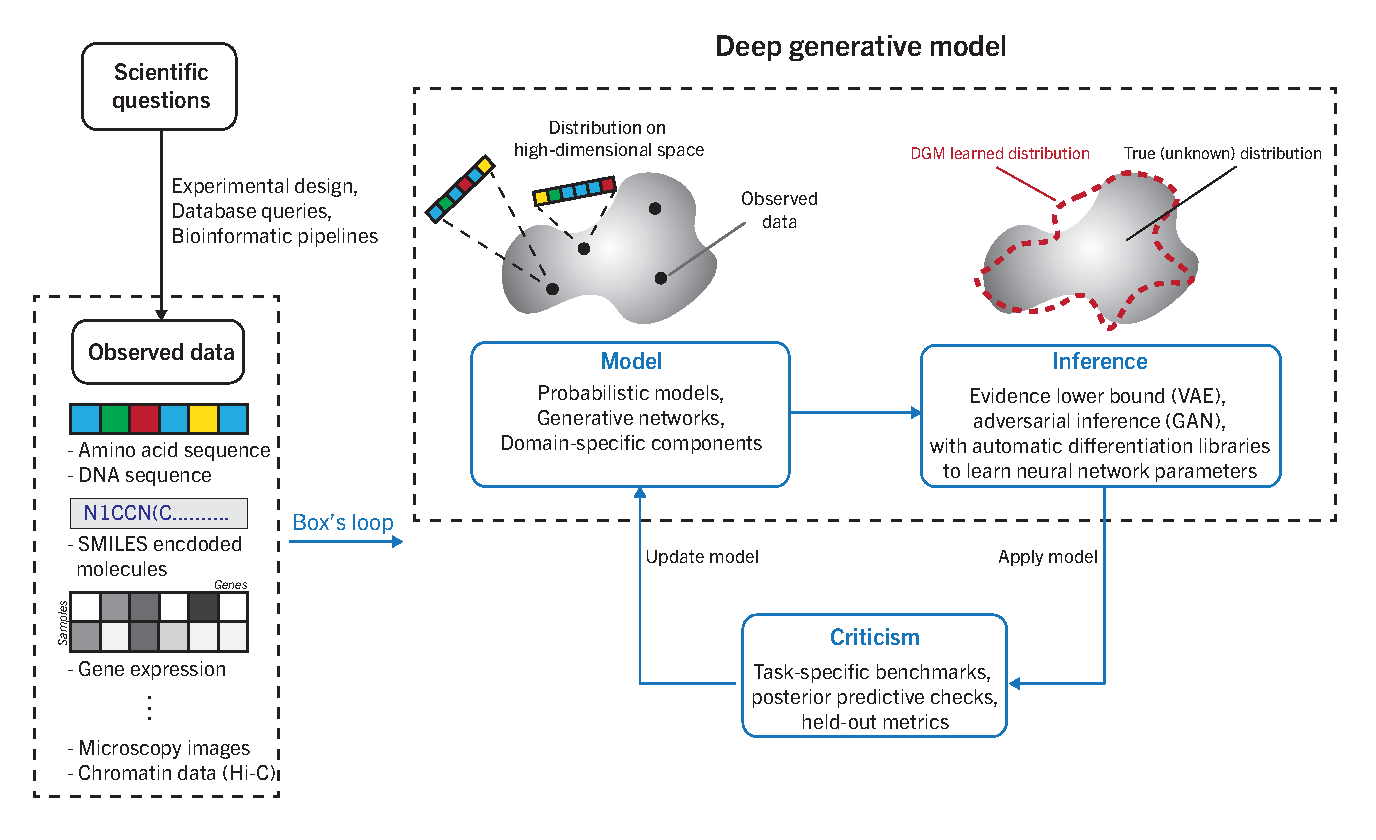
\includegraphics[width=\textwidth]{review/figures/overview_fig.pdf}
    \caption[Overview of the modeling process with DGMs.]{Overview of the modeling process with DGMs. Research in molecular biology stems from the formulation of hypotheses. Such question can be studied through the lens of a wide variety of data forms such as biological sequences, molecules, gene expression or imaging data. The broad goal of a DGM is to estimate the distribution that generated the observed data. Constructing a DGM involves iterating through the steps of Box's loop. First, a model with domain-specific components or assumptions is designed. Second, an inference procedure learns the optimal model parameters. Third, the model is criticized, which consists of benchmarking the model on datasets, or evaluating the goodness of fit of the model. Finally, the model is updated based on the criticism, starting a new iteration of the loop.}
    \label{fig:overview}
\end{figure}

\section{Designing generative models}
\label{subsec:design}
The steps to construct a generative model are best described by Box's loop~\cite{Blei2014} (\textbf{Figure~\ref{fig:overview}}). This procedure, originally proposed by George Box and colleagues~\cite{Box1976,Box1962}, traverses through the main steps of most applications: choosing a model (e.g., selecting the model type, the input covariates, and the distributions that describe these covariates), inferring parameter values (i.e., training), and criticizing the trained model (e.g., evaluating its accuracy on various tasks). After criticism, we return to the first step and iterate through the loop until we are ready to ``deploy'' our model.

An important consideration during model design is its \textit{interpretability} -- in the sense that its parameters will either be immediately useful (e.g., quantifying interactions between pairs of amino-acids~\cite{Riesselman2018}) or can be used in downstream analysis to extract knowledge (e.g., cell to cell similarity~\cite{Lopez2018}). It is often the case that there is a clear trade-off between model complexity and interpretability. Generative models that consist solely of linear operations (such as linear discriminant analysis or factor analysis) are easily interpretable since their parameters normally pertain directly to the input covariates (e.g., one coefficient per gene). This desirable property, however, comes at the cost of a limited ability to fit the data closely. Alternatively, models that use non-linear operations in neural networks (such as VAEs) are normally treated as black-boxes whose parameters are not interpretable. These models, however, usually provide a better fit to the observed data and an increased capacity to generalize upon it~(e.g.,~\cite{Riesselman2018}). The choice of the right trade-off therefore depends on the prospective uses of the model.

Next, we perform inference over the parameters (i.e., fit the model to data). Since exact inference is usually impossible for most types of generative models, one usually has to rely on approximate inference schemes. In this thesis, we focus on specific flavors of approximate inference that relies on neural networks as a way to achieve this. Our choice is motivated by a slew of theoretical and engineering advances that make the task of training generative models significantly more approachable than in the past.


Once the model is fit to the data, an important next step is model criticism. This is achieved by defining a set of attributes that we would like our model to have and a set of metrics to evaluate these attributes. A widely used attribute is the capacity to generalize, namely to properly describe data points that were not available during training. Relevant metrics include the likelihood of held out data points~\cite{wallach2009evaluation} or differences in summary statistics between observed and generated data~(Posterior Predictive Checks, [PPC] \cite{rubin1984bayesianly}). In the latter procedure, we sample random duplicates $\tilde{x}$ of a sample $x^*$ (often a group of samples) from the approximate posterior predictive distribution:
\begin{align}
    p(\tilde{x} \mid x^*) \approx \mathbb{E}_{q(z \mid  x^*)}p(\tilde{x} \mid z),
\end{align}
and compare this to the original data distribution. The comparison can be made by selecting key statistics for the data under scrutiny (e.g., comparing coefficient of variation of each gene in single-cell transcriptomics~\cite{Levitin2019}) and non-parametric tests. These metrics are especially suitable to evaluate Bayesian models but may not be defined for other DGMs.



\section{Encoding knowledge with likelihood-based generative models} 
\label{subsec:encoding_likelihood}
All the generative models in this thesis are explicitly defined via a likelihood function of the observed data. Our goal is to describe a distribution $p_{\theta}(x)$ from which each observation $x$ has been generated, where $\theta$ denotes the parameters of our model. A widely-used way of describing $p_\theta(x)$ with a Bayesian approach is not to model $x$ directly, but instead use an unobserved (latent) random variables $z$ as an intermediary. That is, to generate a new observations $x$ we first draw an intermediary value $z$ from a prior distribution $p_\theta(z)$ and then sample from a likelihood distribution $p_\theta(x\mid z)$~\cite{Wainwright:2008:GME:1498840.1498841}. There are two primary reasons for this modeling strategy. First, conditioning on $z$ allows us to decouple the contribution of individual entries in $x$ (e.g., positions along a sequence) to the overall likelihood of $x$. Since each entry in $x$ it assumed to be independent of all other entries when we condition on $z$, the inference of the parameters $\theta$ becomes substantially simpler. This simplification, for instance, aids DeepSequence to model high-order dependencies between amino acids, going beyond more traditional models~\cite{hopf2017mutation} that account only for pairwise interactions. Second, in many applications $z$ is of much lower dimension than $x$ and can thus provide a concise summary of the data. For instance, in scVI (the core work of this thesis), $z$ represents the cell state in a low dimensional space (typically set to less than $20$ dimensions) that summarizes the high dimensional observations of gene expression (usually thousands of genes). Note that using this property requires a mapping from each observation $x$ back to its representation $z$ in latent space. We discuss one way to achieve this in the next section.

With the use of intermediate variable $z$, the marginal probability (also termed the \emph{evidence}) of a given data set can be formally written by the a combination of the prior $p_\theta(z)$ and likelihood $p_\theta(x\mid z)$:
\begin{align}
\label{factorization}
\log p_\theta(x) = \log\left(\int \left[\prod_{j=1}^dp_\theta(x^j \mid z)\right]p_\theta(z)dz\right),
\end{align}
where $d$ is the dimension of each observation (e.g., length of sequence in DeepSequence) and $x^j$ denotes the $j-$th entry of observation $x$.
Notably, if the prior for $z$ is an isotropic Gaussian distribution:
\begin{align}
    z \sim \mathcal{N}(0, I)
\end{align}
and the likelihood for $x$ is a Gaussian with a linear link:
\begin{align}
    x \mid x \sim \mathcal{N}(u_j^Tz + v_j, \sigma_j^2),
\end{align}
then this formulation is a Bayesian version of principal components analysis (as we are specifying a prior for each entry of the principle components), otherwise known as factor analysis~\cite{Jolliffe1986}. 

While many practical applications indeed fix the prior to be an isotropic Gaussian,
the conditional distributions $p_\theta(x^j\mid z)$ usually come in other forms, which better reflect the nature of the data. For instance, scVI uses negative binomial - a distribution that adequately captures technical~\cite{love2014moderated} and biological~\cite{Grun2014a} noise in the observations of transcript counts. It also includes a possible addition of a zero inflation component to further account for sparseness~\cite{AutoZI}. Finally, scVI also supports the modeling of the conditional distribution $p_\theta(x \mid z, s)$ where $s$ denotes the batch information (treated as an observed random variable). This conditional VAE~\cite{Louizos2016} setting makes it particularly useful for removing of batch effects~\cite{Xu2019}. 

\section{Fitting a generative model using variational inference with neural networks}
\label{subsec:VI_deep}
Once we specified the form of the distributions (prior and likelihood) in our generative model, the inference task is two-fold. First, we would like to find a set of parameters $\theta$ that maximizes the evidence for the data (Equation~\eqref{factorization}). In parallel, for a complete model we would also like to infer the \textit{posterior} distribution $p_\theta(z \mid x)$, which provides a way to represent our observations in the low dimensional latent space. While the parameters $\theta$ can be computed precisely for a restricted choice of distributions (e.g., in factor analysis~\cite{Jolliffe1986} or other cases where the prior is conjugate to the likelihood), exact inference is intractable for most real world applications. Indeed, evaluating the evidence requires integration over the latent variable $z$, which may take exponential time to compute or for which a closed form is not available~\cite{jordan1999introduction}. The same caveat also applies to evaluating the posterior distribution. To see this, recall that Bayes rule entails that:
\begin{align}
\label{eq:Bayesrule}
     p_\theta(z \mid x) = \frac{p_\theta(x \mid z)p_\theta(z)}{p_\theta(x)}.
\end{align}
The numerator in this equation can be readily computed in most applications since the prior and likelihood come with a pre-specified closed form density. However, the denominator is the intractable evidence term.


The main idea behind variational inference is the realization that the problems of maximizing $p_{\theta}(x)$ and approximating $p_{\theta}(z \mid x)$ are very much related. As one way to see this, assume that our goal is to find a distribution $q_{\phi}(z_i)$ (also known as \textit{variational posterior}) that, for a given $\theta$ best approximates the posterior. In other words, for every observation $x_i$, its variational posterior $q_{\phi}(z_i)$ should be as similar as possible to the actual posterior $p_{\theta}(z \mid x_i)$. Because the evidence decomposes across datapoints, we present here the derivation for the evidence of a unique observation. Using Bayes rule, we have for each value of~$z$: 
\begin{align}
    \log p_\theta(x) &= \log \frac{p_\theta(x \mid z)p_\theta(z)}{p_\theta(z \mid x)}.  \label{eq:logBayes} 
\end{align}
We can therefore take expectation of both sides of Equation~\eqref{eq:logBayes} with respect to $q_\phi(z)$ to decompose the evidence as:
\begin{align}
    \log p_\theta(x) &= \mathbb{E}_{q_\phi(z)} \log \frac{p_\theta(x \mid z)p_\theta(z)}{p_\theta(z \mid x)}\\
    &= \mathbb{E}_{q_\phi(z)} \log \left(\frac{p_\theta(x \mid z)p_\theta(z)}{q_\phi(z)}. \frac{q_\phi(z)}{p_\theta(z \mid x)}\right) \\
    &= \mathbb{E}_{q_\phi(z)}\log \frac{p_\theta(x \mid z)p_\theta(z)}{q_\phi(z)} + \mathbb{E}_{q_\phi(z)}\log \frac{q_\phi(z)}{p_\theta(z \mid x)}  \\
    &= \underbrace{\mathbb{E}_{q_\phi(z)} \log \frac{p_\theta(x \mid z)p_\theta(z)}{q_\phi(z)}}_{\text{Evidence lower bound (ELBO)}} +\underbrace{ \kl{q_\phi(z)}{p_\theta(z \mid x)}}_{\text{Variational gap}}, \label{eqn:ELBO_decomp}
\end{align}
where $\Delta_\textrm{KL}$ denotes the Kullback-Leibler (KL) divergence, a notion of similarity between probability distribution. In Equation~\eqref{eqn:ELBO_decomp}, the variational gap quantifies how well $q_\phi(z)$ approximates the posterior and is always positive because that is the KL divergence between two distributions. Consequently, the ELBO is indeed a valid lower bound on the evidence.

Variational inference avoids the intractability of the evidence by maximizing the ELBO, which helps address both of our inference problems. 
The ELBO includes two sets of parameters. The first set $\theta$ controls the generative model and the second set $\phi$ controls the variational approximation to the posterior. Maximizing the ELBO with respect to $\phi$ for a fixed $\theta$ yields an approximation to the posterior $p_\theta(z \mid x)$ and the ELBO approaches the marginal probability $p_{\theta}(x)$. In practice, however, we do not have $\theta$ and the optimization procedure includes assignments of values to both the generative model parameters $\theta$ and the variational posterior parameters $\phi$ so as to maximize the respective ELBO. 


While the ELBO optimization problem is well-studied~\cite{Blei2017}, recent advances in the field provide an effective way to address it using stochastic optimization~\cite{Hoffman2013} as well as neural networks, leading to substantial increase in scalability and (for large enough data sets) accuracy. 
A notable way to achieve this is with \textit{variational autoencoders}~\cite{Kingma2014,Rezende2014}.

\section{Variational auto-encoders}\label{box:VAE}
VAEs provide a way for explicitly representing and then jointly inferring both the variational posterior and the generative model.  A standard VAE model consists of two components (Figure~\ref{vae_fig}): an \textit{encoder} neural network that maps any given point in the observation space ($x_i$) to its corresponding location in latent space ($z_i$). The mapping is done by setting the parameters of the variational posterior $q_{\phi}(z_i)$ for any given observation $x_i$ through a function $f_\phi$ represented by the encoder network. In this notation, $\phi$ refers to the weights of the encoder network. For example, with a Gaussian variational approximation $q_{\phi}(z_i) = \textrm{Normal}\left(\mu_i, \textrm{diag}(v_i)\right)$, we have $(\mu_i, v_i) = f_\phi(x_i)$. Because we can compute $\mu_i$ and $v_i$ with a neural network, we do not need to store these values in memory (by opposition to classical variational inference). Notably, because we can obtain the values of the variational parameters at any observation $x$ (using the encoder network), we refer to the variational distribution as $q_\phi(z \mid x)$. The second component is a \textit{decoder} neural network that maps any given point in the latent space ($z$) to the space of observations ($x$). The mapping is done by setting the parameters of the generative model $p_{\theta}(x \mid z)$. 
\begin{figure}\centering
    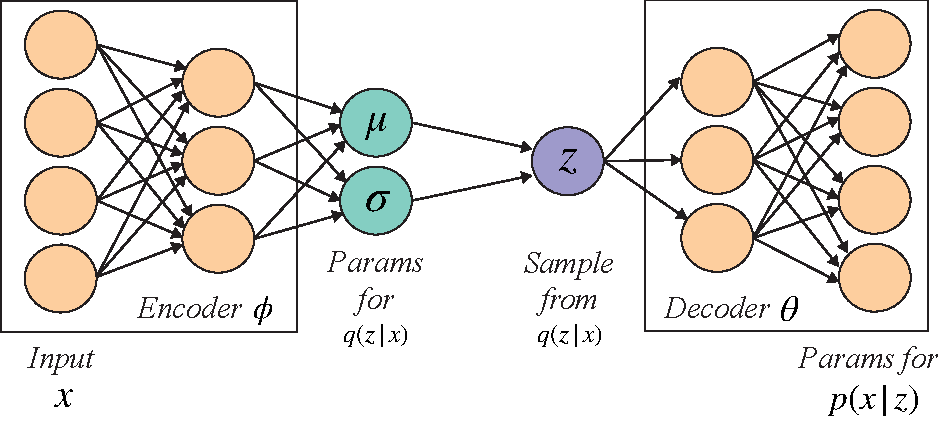
\includegraphics[width=0.6\textwidth]{review/figures/vae.pdf}\\
      \caption{\label{vae_fig}Computational Schematics of the VAE}
\end{figure}
      
A rich literature surrounds the VAE, both in applications and methods development. For instance, the VAE has been applied to image generation~\cite{Gregor2015}, object segmentation with partial observation~\cite{Sohn2015} and astronomy~\cite{AAAI1714765}. Others have focused on improving parts of the framework such as a different (possibly tighter) lower bound~\cite{Li2016,Burda2016}, better posterior approximation~\cite{Kingma2016a}, more flexible choices of distributions~\cite{Ruiz2016} and richer family of graphical models~\cite{NIPS2016_6379}.




\part{Bayesian Models for Single-cell Transcriptomics}
\label{part1}

\chapter{Large-scale Analysis of Single-cell Transcriptomics}
\chaptermark{Single-cell Variational Inference}
\label{scvi}
\section{Introduction}
Single-cell RNA sequencing (scRNA-seq) is a powerful tool that is beginning to make important contributions to diverse research areas such as
development~\cite{Semrau2017},  autoimmunity~\cite{Gaublomme2015}, and cancer~\cite{Patel2014}.
Interpreting scRNA-seq remains challenging, however, as the data is confounded by nuisance factors such as variation in capture efficiency and sequencing depth~\cite{vallejos2017normalizing}, amplification bias, batch effects~\cite{shaham2017removal} and transcriptional noise~\cite{wagner2016revealing}. To avoid mistaking nuisance variation for relevant biological diversity, one must therefore account for measurement bias and uncertainty, especially due to the highly abundant false negatives or ``dropout'' events~\cite{kharchenko2014bayesian}.

The challenge of modeling bias and uncertainty in single-cell data has been explored in several recent studies. A common theme in these studies is treating each data point (cell $\times$ gene) as a random variable and fitting a parametric statistical model to this variable. Most existing models are a mixture of an ``expression'' component, which is usually a negative binomial (e.g., ZINB-WaVE~\cite{zinbwave}) or log normal (e.g., BISCUIT~\cite{biscuit}, and a zero (or low expression) component. The parameters of the model are determined by a combination of cell- and gene-level coefficients, and in some cases additional covariates provided as metadata (e.g., biological condition, batch, and cell quality~\cite{zinbwave}). All of these methods can therefore be interpreted as finding a low-dimensional representation of the data which can be used to approximate the parameters of the cell $\times$ gene random variables. Once these models have been fit to the data, they can then in principle be used for various downstream tasks such as normalization (e.g., scaling, correcting batch effects), imputation of missing data, visualization and clustering.

A complementary line of studies focuses on only one of these tasks, often without explicit probabilistic modeling. For instance, SIMLR~\cite{Wang2017} fits a cell-cell similarity matrix, under the assumption that this matrix has a block structure with a fixed number of clusters. The resulting model can be used for clustering and for visualization~\cite{vanDerMaaten2008}. MAGIC~\cite{magic} performs imputation of unobserved (dropout) counts by propagation in a cell-cell similarity graph. Census~\cite{Qiu2017} and SCNorm~\cite{Bacher2017} look for proper scaling factors by explicitly modeling the dependence of gene expression on sequencing depth or spike-in RNA. For differential expression analysis, the most common methods consist of both methods developed for bulk count data (e.g., DESeq2~\cite{deseq2} and edgeR~\cite{edgeR}) as well as methods developed for scRNA-seq data, explicitly accounting for the high dropout rates (e.g., MAST~\cite{mast}). In~\cite{Lin2017}, neural networks are used as function approximators reducing the dimension of single-cell RNA sequencing data; however, this model is a supervised learning method and inherently relies on some labeling of the cells.

While these methods yield insights into biological variation in single-cell data, several significant limitations remain. First, all of the existing distributional modeling methods assume that a low-dimensional manifold underlies the data, and that the mapping from this manifold to the parameters of the model can be captured by a generalized linear model. While the notion of a restricted dimensionality is plausible (reflecting, for example, common regulatory mechanisms among genes or common states among cells), it is difficult to justify the assumption of linearity. Second, different existing methods use their fitted models for different subsets of tasks (e.g., imputation and clustering, but not differential expression~\cite{biscuit}).  Ideally, one would have a single distributional model that would be used for a range of downstream tasks, thus help ensuring consistency and interpretability of the results. Finally, computational scalability is increasingly important. While most existing methods can be applied to no more than tens of thousands of cells, the next generation of tools must scale to the size of recent data sets (commercial~\cite{10x}, or envisioned by consortia such as the Human Cell Atlas~\cite{Regev2017}) that consist of hundreds of thousands of cells or more. 

To address these limitations, we developed a fully probabilistic approach to normalization and downstream analysis of scRNA-seq data, which we refer to as Single-cell Variational Inference (scVI). scVI is based on a hierarchical Bayesian model~\cite{GelmanHill:2007}.
For each cell, a low-dimensional random vector represents its underlying state. Conditional on this state, each observed gene expression level follows a zero-inflated negative binomial (ZINB) distribution, which captures both overdispersion and dropout events~\cite{Grun2014,deseq2,zinbwave}. The parameters of each ZINB distribution are a nonlinear function of the cell state. We implement this function with deep neural network.

We infer cell states under this model using another deep neural network, known as an encoder network~\cite{kingma2013}. It maps the scRNA-seq data to an approximation of the posterior distribution.
The weights of both neural networks are learned from training data through variation inference~\cite{blei2017variational}, which is a computationally efficient alternative to Markov chain Monte Carlo. 

In the remainder of this chapter, we demonstrate the extent to which scVI addresses the current methodological limitations. First, we demonstrate the scalability of scVI to data sets of up to a million cells. Second, we show that, by using non-linear transformations, scVI better fits unseen data (imputation and held-out log-likelihood). Finally, we demonstrate that the model of scVI can be used for a number of tasks, including batch removal and normalization, clustering, dimensionality reduction and visualization, and differential expression. For each of these tasks, we show that scVI compares favorably to the current state-of-the-art methods. scVI is publicly available at
\url{https://github.com/YosefLab/scvi-tools}. An implementation for all of the analysis performed in this chapter is available at \url{https://zenodo.org/badge/latestdoi/125294792}.

\section{Overview of single-cell Variational Inference (scVI)}
\subsection{Model definition}

The primary output of an scRNA-seq experiment is an $N \times G$-matrix $x$ that records the number of transcripts measured for each of $G$ genes in each of $N$ cells. We may also have a batch annotation $s_n$ observed for each cell $n$ as well.

We model the  expression level $x_{ng}$ measured for each cell $n$ and gene $g$ as a sample drawn from a conditional distribution that has a zero-inflated negative binomial (ZINB) form \cite{Grun2014,deseq2,zinbwave}. The distribution is conditioned on the observed batch annotation, as well as  two additional, unobserved random variables. The latent random variable $\ell_n$ represents nuisance variation due to variation in capture efficiency and sequencing depth. It is drawn from a log-normal distribution and serves as a cell-specific scaling factor. %Notably, the heavy tail property of $\ell_n$ makes the distribution of gene expression richer and better removes the variation in gene expression coming from library size. %%Not sure about this one. This might open up for a reviewer's question

The latent random variable $z_n$ represents the remaining variability, which should better reflect biological differences between cells. It is drawn from a standard multivariate normal of low dimensionality $d$, and provides a latent-space representation that can be used for visualization and clustering.
The matrix $\rho$ is an intermediate value that relates the observations $x_{ng}$ to the latent variables. It provides a batch-corrected, normalized estimate of the percentage of transcripts in each cell $n$ that originate from each gene $g$. We use $\rho$ for differential expression analysis and its scaled version (multiplying by the estimated library size) for imputation.

Altogether, each expression value $x_{ng}$ is drawn independently through the following process:
\begin{align}
	z_n &\sim \textrm{Normal}(0, I) \\
    \ell_n &\sim \textrm{LogNormal}(\ell_\mu, \ell_\sigma^2) \\
    \rho_n &= f_w(z_n, s_n) \\
    w_{ng} &\sim \mathrm{Gamma}(\rho_n^g, \theta) \\
    y_{ng} &\sim \mathrm{Poisson}( \ell_n w_{ng}) \\
    h_{ng} &\sim \mathrm{Bernoulli}(f_h^g(z_n, s_n)) \\
    x_{ng} &=
\begin{cases}
y_{ng} & \text{ if } h_{ng} = 0,\\
0 & \text{ otherwise}.\\
\end{cases}
\end{align}
A standard multivariate normal prior for $z$ is commonly used in variational autoencoders since it can be reparametrized in a differentiable way into any arbitrary multivariate Gaussian random variable~\cite{kingma2013}, which turns out to be extremely convenient in the inference process. 

$B$ denotes the number of batches and $\ell_\mu, \ell_\sigma \in \mathbb{R}_+^B$ parameterize the prior for the scaling factor (on a log scale), and are set to be the empirical mean and variance of the log-library size per each batch. Let us note that the random variable $\ell_n$ is not the log-library size (scaling the sampled observation) itself but a scaling factor that is expected to correlate strongly with log-library size (hence the choice of the parameters).

The parameter $\theta \in \mathbb{R}_+^G$ denotes a gene-specific inverse dispersion, are estimated as global parameters estimated via variational Bayesian inference. $f_w$ and $f_h$ are neural networks that map the latent space and batch annotation back to the full dimension of all genes: $\mathbb{R}^d\times\{0, 1\}^B \rightarrow \mathbb{R}^G$ (Figure 1b, NN5-6). We use superscript annotation (e.g., $f_w^g(z_n, s_n)$) to refer to a single entry that corresponds to a specific gene $g$. We apply a softmax activation at the last layer of $f_w$. Therefore, $f_w^g(z_n, s_n)$ to take values in the probability simplex (namely, for each cell $n$ the sum of $f_w^g(z_n, s_n)$ values over all genes $g$ is one), and may be interpretated as expected frequencies. Neural network $f_h$ encodes whether a particular entry has been dropped out due to technical effects~\cite{zifa,zinbwave}. Importantly, neural networks allows us to go beyond the generalized linear model framework and provide a more flexible model of gene expression. Figure \ref{scviPanel1}a specifies the complete graphical model and its implementation using neural-network conditionals.

All neural networks use dropout regularization and batch normalization. Each network has 1, 2, or 3 fully connected-layers, with 128 or 256 nodes each. The activation functions between two hidden layers are all ReLU. We use a standard link function to parametrize the distribution parameters (exponential, logarithmic or softmax). Weights for some layers are shared between $f_w$ and $f_h$. 

\begin{figure}
    \centering
    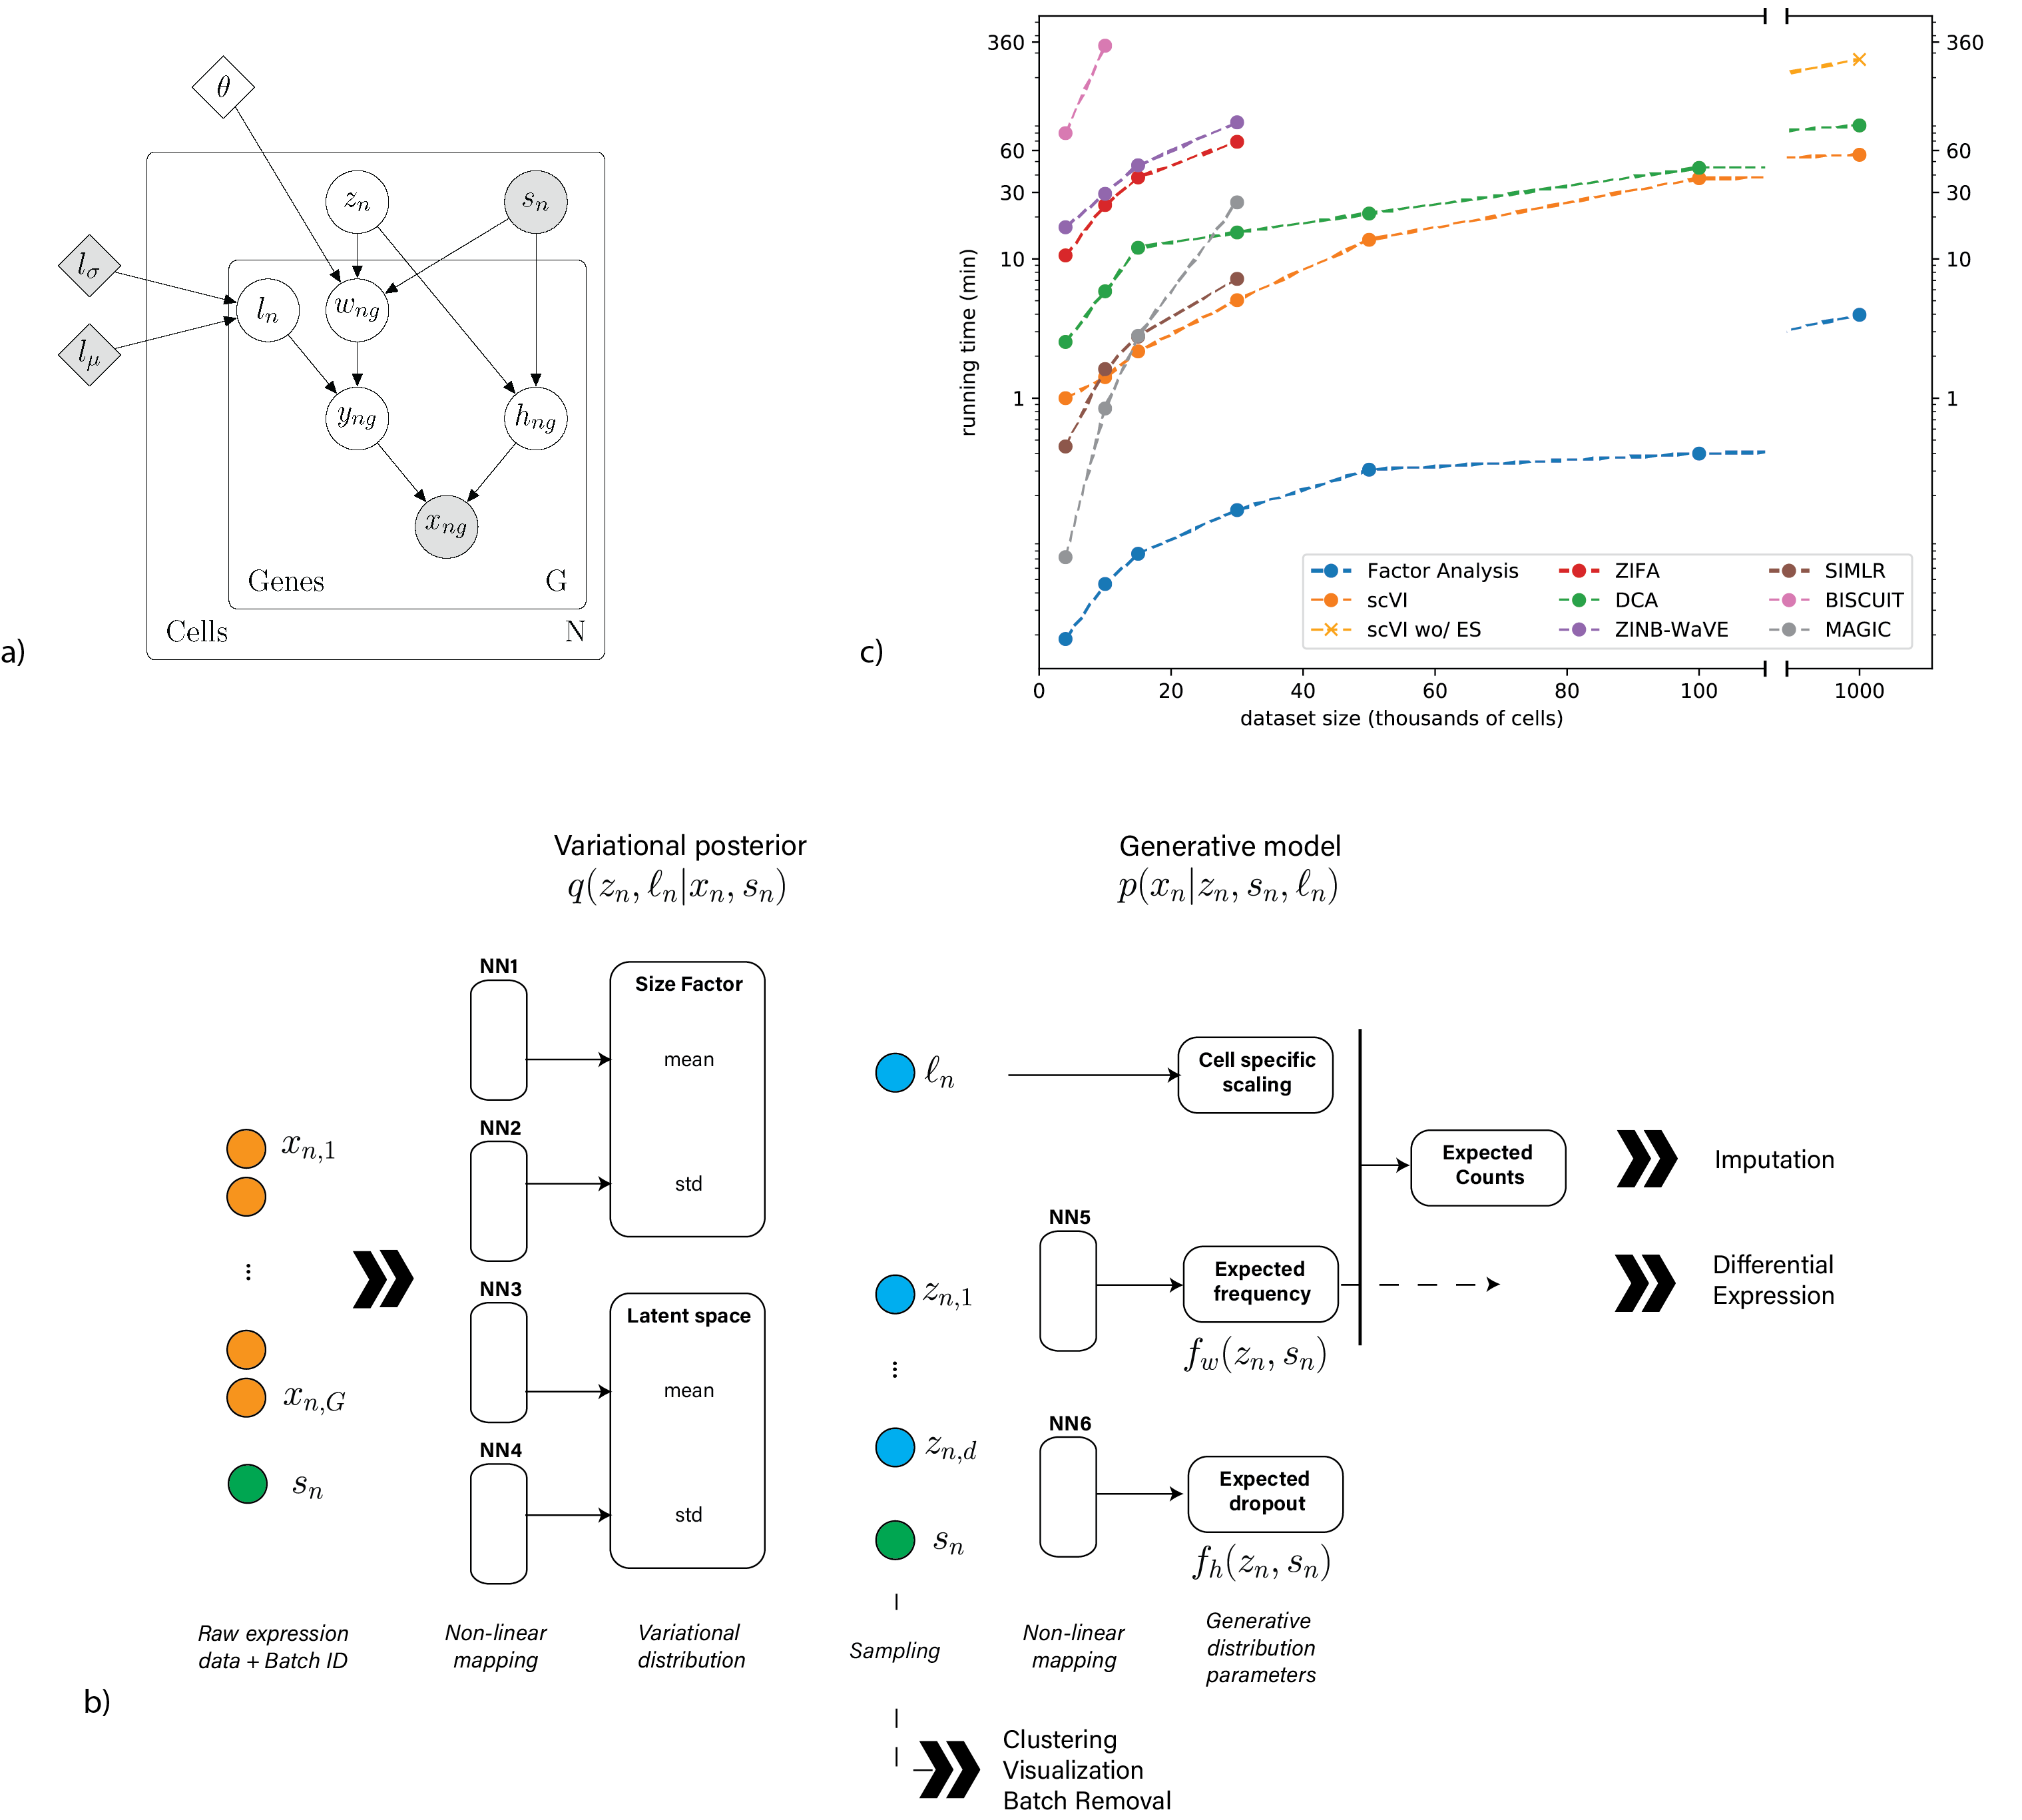
\includegraphics[width=0.9\textwidth]{figures/Figure-1.png}
    \caption[Overview of scVI]{Overview of scVI. Given a gene-expression matrix with batch annotations as input, scVI learns a non-linear embedding of the cells that can be used for multiple analysis tasks. (a) The underlying graphical model. Shaded vertices represent observed random variables. Empty vertices represent latent random variables. Shaded diamonds represent constants, set a priori. Empty diamonds represent global variables shared across all genes and cells. Edges signify conditional dependency. Rectangles (``plates'') represent independent replication. (b) The computational trees (neural networks) used to compute the embedding as well as the distribution of gene expression. (c) Comparison of running times (y-axis) on the BRAIN-LARGE data with a limited set of 720 genes, and with increasing input sizes (x-axis; cells in each input set are sampled randomly from the complete dataset). scVI is compared against existing methods for dimensionality reduction in the scRNA-seq literature. As a control, we also add basic matrix factorization with factor analysis (FA). For the one-million-cell dataset only, we report the result with and without early stopping (ES).}
    \label{scviPanel1}
    \end{figure}
    

\subsection{Fast inference via stochastic optimization}
The posterior distribution combines the prior knowledge with information acquired from the data $X$. We cannot directly apply Bayes rule to determine the posterior because the denominator (the marginal distribution) $p(x_n \mid s_n)$ is intractable. We therefore proceed to deriving a variational inference recipe. 

\subsubsection{Partial analytical integration of latent variables}
Making inference over the whole graphical model is not needed. We can integrate out the latent variables $w_{ng}$, $h_{ng}$ and $y_{ng}$ by ensuring the conditional $p(x_{ng} \mid z_{n}, \ell_{n}, s_n)$ has a closed-form density and is zero-inflated negative binomial. The result follows from analytical integration:

\begin{restatable}{lemma}{lemmazinb}\emph{(Marginalizing the latent variables of scVI)}\label{lemma:zinb}
    The conditional distribution $p(x_{ng} \mid z_{n}, \ell_{n}, s_n)$ follows a zero-inflated negative binomial distribution of mean $\ell_{n}f^g_w(z_n, s_n)$, dispersion $\theta_g$ and mixture weight $f^g_h(z_n, s_n)$.
    \end{restatable}
\begin{proof}
    For this proof, we need to first apply a standard result on Gamma poisson compounds, and then carefully identify the zero probability. 
    \paragraph{Step 1: integrating the Gamma latent variable} Let $r$ to be the gene-specific shape parameter of a Gamma variable $w$ and let $\frac{p}{1-p}$ be its scale parameter. For any scalar $\lambda \in \mathbb{R}^+$, the random variable defined by $y \mid w \sim \textrm{Poisson}(\lambda w)$ has a negative binomial marginal distribution with mean $\lambda\frac{rp}{1-p}$ and shape $r$:
\begin{align}
 p(y) &= \int p(y \mid w) p(w)dw  \\
 &= \int \frac{w^{r-1} e^{-w(\frac{1}{p}-1)}(1-p)^r}{p^r\Gamma(r)}\frac{e^{-\lambda w} \lambda^y w^y}{\Gamma(y+1)}dw \\
&= \frac{\Gamma(y + r)}{\Gamma(y+1)\Gamma(r)} \left(\frac{1-p}{1-p + \lambda p} \right)^r \left(\frac{p\lambda}{1-p + \lambda p} \right)^y \\
&= \textrm{NegativeBinomial}\left(y; \lambda\frac{rp}{1-p}, r\right).
\end{align}
\paragraph{Step 2: identifying the zero-probability}
Multiplication by zero to $y_{ng}$ can be formally encoded as a mixture between a point-mass at zero and the original distribution of $y_{ng}$. Then, our conditional $p(x_{ng} \mid z_{n}, \ell_{n}, s_n)$ is a zero-inflated negative binomial:
\begin{align}
       p(x_j = 0 \mid z, l, s) &= f_h(z)_j + (1 - f_h(z)_j) \left( \frac{\theta_j}{\theta_j + l f_w(z)_j } \right)^{\theta_j}
\end{align}
and
\begin{align}
      p(x_j = y \mid z, l, s) &= (1-f_h(z)_j) \frac{\Gamma(y + \theta_j)}{\Gamma(y+1)\Gamma(\theta_j)} \left( \frac{\theta_j}{\theta_j + l f_w(z)_j } \right)^{\theta_j} \left( \frac{lf_w(z)_j}{\theta_j + l f_w(z)_j } \right)^y.
\end{align}
Here $f_h(z)$ encodes the zero probability of $h$ and $f_w(z)$ the mean of $w$.
\end{proof}

\subsubsection{Amortized variational inference}
Having simplified our model, we use variational inference~\cite{blei2017variational} to approximate
the posterior $p(z_n, \ell_n \mid x_n, s_n)$. Our variational distribution $q(z_n, \ell_n \mid x_n, s_n)$ is mean-field:
\begin{align}
    q(z_n, \ell_n \mid x_n, s_n) = q(z_n \mid x_n, s_n)q(\ell_n \mid x_n, s_n).
\end{align}

The variational distribution $q(z_n \mid x_n, s_n)$ is chosen to be Gaussian with a diagonal covariance matrix, mean
and covariance given by an encoder network applied to $(x_n, s_n)$, as in~\cite{kingma2013} (Figure 1b, NN1-4)). The variational distribution $q(\ell_n \mid x_n, s_n)$ is chosen to be log-normal with the scalar mean and variance also given by an encoder network applied to $(x_n, s_n)$. The variational lower bound is:
\begin{equation}\label{scvivar_bound}
\begin{split}
\log p(x_n \mid s_n) \geq & \mathbb{E}_{q(z_n, l_n\mid x_n, s_n)}\log p(x_n\mid z_n, l_n, s_n)  \\
& \qquad- \kld{q(z_n\mid x_n, s_n)}{p(z_n)} \\
& \qquad - \kld{q(l_n\mid x_n, s_n)}{p(l_n)}.
\end{split}
\end{equation}

In this objective function, the dispersion parameters $\theta_g$ for each gene  are treated as global variables to optimize in a Variational Bayesian inference fashion. To optimize the lower bound, we use the analytic expression for $p(x_n\mid z_n, l_n, s_n)$ and use analytic expressions for the Kullback-Leibler divergences. We use the reparametrization trick to compute low-variance Monte-Carlo estimates of the expectations' gradients. Analytic closed-form for the Kullback-Leibler divergence and the reparametrization trick are only possible on certain distributions which multivariate Gaussians are a part of~\cite{kingma2013}. Now, our objective function is continuous and end-to-end differentiable, which allows us to use automatic differentiation operators. As indicated in \cite{Sønderby2016}, we use deterministic warmup and batch normalization during learning to learn an expressive model.

Since our model assumes cells are identically independently distributed, we can also benefit from stochastic optimization by sampling the training set. We then have an online optimization procedure that can handle massive datasets. At each iteration, we focus only on a small subset of the data randomly sampled ($M = 128$ data points) and do not need to go through the entire dataset. Therefore, there is no need to store the entire dataset in memory. Because the number of genes is  in practice limited to a few tens of thousands, these mini-batches of cells fit easily into a GPU.

Since the encoder network $q(z \mid x, s)$ might still produce output correlated with the bath $s$, we use a Maximum Mean Discrepancy (MMD) based penalty as in \cite{louizos2016variational} to correct the variational distribution. For this chapter, however, we did not explicitly enforce the MMD penalty and simply retained the conditional independence property, which has shown to be sufficiently efficient. This may be useful on other datasets.

\subsection{Choice of hyperparameters}
Throughout the chapter, we use Adam (a first order stochastic optimizer) with $\epsilon = 0.01$. A complete list of datasets and their properties, the methods we applied, and a complete list of hyperparameters is provided in Table \ref{scvidatasets}. The hyperparameters were chosen using a small grid search that maximized held-out log likelihood---a common practice for training deep generative models. One of the strengths of scVI is that we have only three dataset-specific hyperparameters to set (learning rate, number of layers, and layer width). We optimize the objective function until convergence  --usually between 120 and 250 epochs, where each epoch is a complete pass through the dataset (let us note that bigger datasets require fewer epochs). For the larger subset of the BRAIN-LARGE dataset, we also ran with the early stopping criterion: the algorithm stops after 12 consecutive epochs with no improvement on the loss. 


\begin{table}
    \centering
    \resizebox{\textwidth}{!}{
        \begin{small}
    \begin{tabular}{lcccccccccc}
    \toprule

                                                                   & \multicolumn{2}{c}{\textbf{dataset properties}} & \multicolumn{3}{c}{\textbf{scVI hyperparameters}}                                                     & \multicolumn{5}{c}{\textbf{scalability to other algorithms}}                                                                 \\
    \textbf{}                                                      & \textbf{cells}         & \textbf{genes}         & \textbf{\begin{tabular}[c]{@{}l@{}}learning\\ rate\end{tabular}} & \textbf{layers} & \textbf{neurons} & \textbf{FA} & \textbf{ZIFA} & \textbf{\begin{tabular}[c]{@{}l@{}}ZINB\\ WaVE\end{tabular}} & \textbf{MAGIC} & \textbf{SIMLR} \\
    \midrule \\
    \textbf{CORTEX}                                                & 3,005                  & 558                    & 0.0004                                                           & 1               & 128              & \_          & \_            & \_                                                           & \_             & \_             \\[0.2cm]
    \textbf{PBMC}                                                  & 12,039                 & 3,346                  & 0.0004                                                           & 1               & 128              & \_          & x             & x                                                            & \_             & \_             \\[0.2cm]
    \textbf{HEMATO}                                                & 4,016                  & 7,397                  & 0.0004                                                           & 1               & 128              & \_          & x             & x                                                            & \_             & NC             \\[0.2cm]
    \textbf{HEMATO$^*$}                                                & 4,016                  & 700                  & 0.0004                                                           & 1               & 128              & \_          & x             & x                                                            & \_             & NC             \\[0.2cm]
    \textbf{\begin{tabular}[c]{@{}l@{}}BRAIN\\ LARGE\end{tabular}} & 10,000                 & 720                    & 0.001                                                            & 1               & 128              & \_          & \_            & \_                                                           & \_             & NA             \\[0.4cm]
    \textbf{\begin{tabular}[c]{@{}l@{}}BRAIN\\ LARGE\end{tabular}} & 15,000                 & 720                    & 0.001                                                            & 2               & 128              & \_          & \_            & \_                                                           & NC             & NA             \\[0.4cm]
    \textbf{\begin{tabular}[c]{@{}l@{}}BRAIN\\ LARGE\end{tabular}} & 50,000                 & 720                    & 0.001                                                            & 3               & 256              & \_          & x             & x                                                            & NC             & NA             \\[0.4cm]
    \textbf{\begin{tabular}[c]{@{}l@{}}BRAIN\\ LARGE\end{tabular}} & 1M                     & 720                    & 0.001                                                            & 3               & 256              & \_          & x             & x                                                            & x             & NA             \\[0.4cm]
    \textbf{\begin{tabular}[c]{@{}l@{}}BRAIN\\ LARGE\end{tabular}} & 1M                     & 10,000                    & 0.001                                                            & 3               & 256              & \_          & x             & x                                                            & x             & NA             \\[0.4cm]
    \textbf{RETINA}                                                & 27,499                 & 13,166                 & 0.0005                                                           & 1               & 128              & \_          & x             & x                                                            & x              & \_             \\[0.2cm]
    \textbf{CBMC}                                                  & 8,617                  & 600                    & 0.0005                                                           & 1               & 128              & \_          & \_            & \_                                                           & NC             & \_             \\[0.2cm]
    \textbf{\begin{tabular}[c]{@{}l@{}}BRAIN\\ SMALL\end{tabular}} & 9,128                  & 3,000                  & 0.001                                                            & 1               & 128              & NC          & NC            & NC                                                           & NC             & NC\\
    \bottomrule
\end{tabular}
\end{small}
    }
    \caption[Presentation of the different datasets, their gene filtering and applicability of algorithms]{Presentation of the different datasets, their gene filtering and applicability of algorithms. ``\_'' indicates combinations of algorithms and datasets that were included in this study. ``x'' indicates that the algorithm took more than four hours to run (ZIFA) or that the computer ran out of memory (others). ``NA'' indicates datasets where pre-annotated subpopulations were not available, which makes them less useful for application with SIMLR and benchmarks of clustering. ``NC'' indicates the remaining combinations of algorithms and datasets that were not considered for this study. For instance, BRAIN-SMALL was only used to study the correlation of scVI zero probabilities and quality parameters (Figure 6).}
    \label{scvidatasets}
    \end{table}
    

    


\subsection{Related variational autoencoder works}
Independently of our work, several recent articles and preprints have also described the use of neural networks, including variational autoencoders~\cite{kingma2013} (VAEs), to embed scRNA-seq datasets. Like scVI, these methods use stochastic optimization and therefore also scale to the size of recent data sets. 
scVI stands apart from this research in its focus on separating technical effects from biological signals. To this end, we explicitly model library size and batch effects as nuisance variables in a hierarchical Bayesian model. Empirical advantages of such careful modeling are underlined in~\cite{biscuit,basics} for library size and~\cite{zinbwave,SCONE} for batch effects. scVI is also distinguished by the large variety of datasets it has been validated on, and the number downstream applications it supports (see Table~\ref{scvialgorithms_pres}). In the following, we provide a brief description of each method.

scvis~\cite{scvis} proposes a new variational lower bound inspired by the parametric version of tSNE for single-cell visualization. Unlike scVI, scvis uses principal component analysis for preprocessing the data, and relies on $t$-distributed conditional distributions. These assumptions may be fruitful for visualization purposes but may not help in recovering hidden gene expression levels for either imputation or differential expression. One notable reason is that the underlying statistical assumptions for applying principal component analysis are not verified in the scRNA-seq dataset and the output of this preprocessing may have artifacts~\cite{zinbwave}.

VASC~\cite{VASC} adds zero-inflation to a VAE with Gaussian conditional distributions and shows competitive performance on clustering. Preprocessing relies on normalizing the data by library size in order to suit their loss function. However, it is known that size scaling normalization can induce bias in the analysis~\cite{vallejos2017normalizing} and that count distributions such as ZINB outperform zero-inflated Gaussian conditional distribution for modeling and downstream analysis~\cite{zinbwave, zifa}.

DCA~\cite{dca} is a denoising auto-encoder~\cite{VincentPASCALVINCENT2010} that proposes a ZINB loss function. The output of this algorithm is a latent space as well as a point estimate for the conditional distributions (this denoising method is essentially a non-linear version of ZINB-WaVE). However, it is hard to extend this method for differential expression without the possibility of posterior sampling. Notably, library size discrepancies are also corrected via size scaling and potentially hurt downstream analysis~\cite{vallejos2017normalizing}.

scVAE~\cite{scVAE} proposes to use VAEs with count conditional distributions for Bayesian modeling and clustering analysis. Notably, their work uses (among others) the NB and the ZINB as conditional distributions but do not propose an approach for normalization, which is crucial for further analysis.

\begin{table}
\centering
\resizebox{\textwidth}{!}{
    \begin{small}
\begin{tabular}{lcccccccc}
    \toprule
                         & \multicolumn{5}{c}{\textbf{Characteristics of the Model}}                                                                                                                                                                                                  & \multicolumn{3}{c}{\textbf{Features of the Software}}                                                                                                                            \\
                        \\
                         & \textbf{Dropout} & \textbf{\begin{tabular}[c]{@{}l@{}}Count\\ distribution\end{tabular}} & \textbf{Library size} & \textbf{\begin{tabular}[c]{@{}l@{}}Batch \\ Effects\end{tabular}} & \textbf{\begin{tabular}[c]{@{}l@{}}Generative\\ Model\end{tabular}} & \textbf{\begin{tabular}[c]{@{}l@{}}Dimensionality \\ Reduction\end{tabular}} & \textbf{Imputation} & \textbf{\begin{tabular}[c]{@{}l@{}}Differential\\ Expression\end{tabular}} \\
   \midrule                      
\textbf{Factor Analysis} &                  &                                                                       &                       &                                                                   & X                                                                   & X                                                                            &                     &                                                                            \\[0.2cm]
\textbf{ZIFA}            & X                &                                                                       &                       &                                                                   & X                                                                   & X                                                                            &                     &                                                                            \\[0.2cm]
\textbf{SIMLR}           &   X               &                                                                       &                       &                                                                   &                                                                     & X                                                                            &                     &                                                                            \\[0.2cm]
\textbf{BISCUIT}         &                  &                                                                       & X                     &                                                                   & X                                                                   & X*                                                                           &                     &                                                                            \\[0.2cm]
\textbf{ZINB-WaVE}       & X                & X                                                                     &                       & X                                                                 &                                                                     & X                                                                            & X                   &                                                                            \\[0.2cm]

\textbf{MAGIC}           & X                &                                                                       &                       &                                                                   &                                                                     &                                                                              & X                   &                                                                            \\[0.2cm]

\textbf{DESeq2}          &                  & X                                                                     & X                     & X                                                                 &                                                                     &                                                                              &                     & X                                                                          \\[0.2cm]
\textbf{MAST}            & X                & X                                                                     & X                     & X                                                                 &                                                                     &                                                                              &                     & X                                                                          \\[0.2cm]
\textbf{edgeR}           &                  & X                                                                     & X                     & X                                                                 &                                                                     &                                                                              &                     & X                                                                          \\[0.2cm]

\textbf{ComBat}          &                  &                                                                       &                       & X                                                                 &                                                                     &                                                                              & X                   &                                                                            \\[0.2cm]
\textbf{MNNs}            &                  &                                                                       &                       & X                                                                 &                                                                     &                                                                              & X                   &                                                                            \\[0.2cm]

\textbf{scvis}           &                  &                                                                       &                       &                                                                   & X                                                                   & X                                                                            &                     &                                                                            \\[0.2cm]
\textbf{DCA}             & X                & X                                                                     &                       &                                                                   &                                                                     & X                                                                            & X                   &                                                                            \\[0.2cm]
\textbf{VASC}            & X                &                                                                       &                       &                                                                   & X                                                                   & X                                                                            &                     &                                                                            \\[0.2cm]
\textbf{scVAE}           & X                & X                                                                     &                       &                                                                   & X                                                                   & X                                                                            & X                   &                                                                    \\[0.2cm]


\textbf{scVI}            & X                & X                                                                     & X                     & X                                                                 & X                                                                   & X                                                                            & X                   & X                                                                         \\
\bottomrule
\end{tabular}
\end{small}
}
\caption[Presentation of all the papers cited in this chapter]{Presentation of all the papers cited in this chapter. We describe both features of the model and the corresponding open-source software. \emph{Dropout}: any computing solution to mitigate the dropout effect on data analysis. \emph{Count distribution}: the underlying distribution modeling the gene expression has support in the integer set. \emph{Library size}: the model is designed to correct for library size or other technical effects. \emph{Batch effects} refers to a model that can account for this technical variation. \emph{Generative Model} refers to the possibility of sampling from a posterior. The star ($^*$) for BISCUIT indicates that this algorithm cannot perform dimensionality reduction but can still cluster cells.}
\label{scvialgorithms_pres}
\end{table}



\section{Results}

\subsection{Presentation of the datasets}

We apply scVI to seven publicly available datasets for preprocessing information). We focus on datasets with unique molecular identifiers (UMIs), which prevents overcounting due to amplification. Due to scalability issues, not all of the benchmark methods included in this chapter are applicable to all datasets. A star after the dataset name indicates we used it as an auxiliary dataset; these datasets were not used for general benchmarking, but rather to support specific points presented in the chapter. The only case where we subsampled the data multiple times was the BRAIN-LARGE dataset. However, we simply used one instance of it to report all possible scores (further details in Table~\ref{scvidatasets}).

The first dataset (BRAIN-LARGE) consists of 1.3 million mouse brain cells, spanning the cortex, hippocampus and subventricular zone, and profiled with 10x chromium~\cite{10x}. We use this dataset to demonstrate the scalability of scVI. We randomly shuffle the data to get a 1M subset of cells and order genes by variance to retain first 10,000 and then 720 sampled variable genes. This dataset is then sampled multiple times in cells for the runtime and goodness-of-fit analysis. We report imputation scores on the 10k cells and 720 gene samples only.

The second dataset (CORTEX) consists of 3,005 mouse cortex cells profiled with the Smart-seq2 protocol, with the addition of UMI~\cite{Zeisel1138}. To facilitate comparison with other methods, we use a filtered set of 558 highly variable genes as in~\cite{biscuit}. The CORTEX dataset exhibits a clear high-level subpopulation structure, which has been inferred by the authors of the original publication using computational tools and annotated by inspection of specific genes or transcriptional programs. Similar levels of annotation are provided with the third and fourth datasets. 
    
    
The third dataset (PBMC) consists of 12,039 human peripheral blood mononuclear cells from a healthy donor (4K PBMCs and 8K PBMCs) \cite{Zheng2017}. We derived quality control metrics using the cellrangerRkit R package (v. 1.1.0). Quality metrics were extracted from CellRanger throughout the molecule-specific information file. After filtering as in \cite{SCONE}, we extract 12,039 cells with 10,310 sampled genes and generate biologically meaningful clusters with the software Seurat~\cite{SEURAT}~(see Table~\ref{scvipbmc-celltypes}). We then filter genes that we could not match with the bulk data used for differential expression to be left with $g = 3,346$. 

\begin{table}[ht]
    \centering
    \resizebox{\textwidth}{!}{
        \begin{small}
    \begin{tabular}{lccccc}
        \toprule
    \textbf{Cell Type}             & \textbf{\# cells} & \begin{tabular}[c]{@{}c@{}} \textbf{Cluster ID}    \\ \textbf{(original)}\end{tabular} & \begin{tabular}[c]{@{}c@{}}\textbf{Cluster ID}\\ \textbf{(\#4)}\end{tabular} & \begin{tabular}[c]{@{}c@{}} \bfseries Cluster ID\\ \bfseries (\#3)\end{tabular} & \begin{tabular}[c]{@{}c@{}} \bfseries Cluster ID\\ \bfseries (\#2)\end{tabular} \\
    \midrule
    astrocytes ependymal & 224      & 0                                                                & 1                                                          & 0                                                          & 0                                                          \\
    endothelial-mural     & 235      & 1                                                                & 2                                                          & 1                                                          & 0                                                          \\
    interneurons          & 290      & 2                                                                & 3                                                          & 2                                                          & 1                                                          \\
    microglia             & 98       & 3                                                                & 2                                                          & 1                                                          & 0                                                          \\
    oligodendrocytes      & 820      & 4                                                                & 0                                                          & 0                                                          & 0                                                          \\
    pyramidal CA1         & 939      & 5                                                                & 3                                                          & 2                                                          & 1                                                          \\
    pyramidal SS          & 399      & 6                                                                & 3                                                          & 2                                                          & 1                                                         \\
    \bottomrule
    \end{tabular}
\end{small}
    }
    \caption{Cell types present in the CORTEX dataset and their labels in some slices of the original hierarchical clustering.}
    \label{scvicortex-celltypes}
    \end{table}

\begin{table}[ht]
    \centering
    \begin{small}
    \begin{tabular}{lc}
        \toprule
        \bfseries Cell Types        & \bfseries \# cells \\
    \midrule
    B cells           & 1625     \\
    CD14+ Monocytes   & 2237     \\
    CD4 T cells       & 5024     \\
    CD8 T cells       & 1452     \\
    Dendritic Cells   & 339      \\
    FCGR3A+ Monocytes & 351      \\
    Megakaryocytes    & 88       \\
    NK cells          & 459      \\
    Other             & 464     \\
    \bottomrule
    \end{tabular}
\end{small}
    \caption{Cell types present in the PBMC dataset.}
    \label{scvipbmc-celltypes}
    \end{table}

The fourth dataset (RETINA) includes 27,499 mouse retinal bipolar neurons, profiled in two batches using the Drop-Seq technology~\cite{bipolar}. We filtered 13,166 most variable genes. The original annotations of these datasets were used to benchmark scRNA-seq algorithms in several subsequent studies (e.g.,~\cite{Wang2017,biscuit}). We also extract their normalized data with Combat and use it for benchmarking.

The fifth dataset (HEMATO) includes 4,016 cells from two batches that were profiled using in-drop (7,397 genes captured). This data provides a snapshot of hematopoietic progenitor cells differentiating into various lineages. We use this dataset as an example for cases where gene expression varies in a continuous fashion (along pseudo-temporal axes) rather than forming discrete subpopulations~\cite{Tusi2018}. We removed the library \emph{basal-bm1}, which was of poor quality, based on authors recommendation. We use their population balance analysis~\cite{Weinreb2018} result as a potential function for differentiation. 

The sixth dataset (CBMC$^*$) includes 8,617 cord blood mononuclear cells profiled using 10x along with, for each cell, 13 well-characterized mononuclear antibodies~\cite{Stoeckius2017}. We used this dataset to analyze how the latent spaces inferred by dimensionality-reduction algorithms summarize protein marker abundance. We kept the top 600 genes by variance.

The seventh dataset (BRAIN-SMALL$^*$) consists of 9,128 mouse brain cells profiled using 10x~\cite{10x}. This dataset is used as a complement to PBMC for our study of zero abundance and quality control metric correlation with our generative posterior parameters. We derived quality control metrics using the cellrangerRkit R package (v. 1.1.0). Quality metrics were extracted from CellRanger throughout the molecule-specific information file. We kept the top 3000 genes by variance. We used the clusters provided by cellRanger for the correlation analysis of zero probabilities.


\subsection{Scalability to large datasets}
We start by comparing the scalability of scVI to that of state-of-the-art algorithms for imputation and dimensionality reduction (Figure~\ref{scviPanel1}c). We evaluate scalability in terms of runtime and memory requirements for increasing numbers of cells, sampled from the complete BRAIN-LARGE dataset. To facilitate comparison to less scalable methods, we limited the analysis to the 720 genes with largest standard deviation across all cells. All the algorithms were tested on a machine with one eight-core Intel i7-6820HQ CPU addressing 32 GB RAM, and one NVIDIA Tesla K80 (GK210GL) GPU addressing 24 GB RAM.

Available memory (RAM) limits scalability of many existing algorithms. Under the hardware and input settings above, we find that BISCUIT runs out of memory when provided with more than 15K cells. MAGIC, ZIFA, SIMLR and ZINB-WaVE can process up to 50K cells before running out of memory. One explanation for this is the explicit storage in memory of the full-data matrix or its derivative (e.g., the cell-cell distance matrix or a proxy whose memory complexity is linear in the number of data points, as in SIMLR and MAGIC).

Focusing on the memory-feasible dataset sizes, we also observe a range of runtimes. For instance, ZIFA,  ZINB-WaVE and BISCUIT have relatively high runtime requirements, possibly because their optimization algorithms need to go through all of the training data at each each step: the runtime of each iteration scales linearly in the number of samples and linearly in the number of genes.

scVI relies instead on stochastic optimization, sampling a fixed number of cells at each iteration. Its time and space complexity per iteration therefore depends only on the number of genes, ensuring scalability both in terms of memory use and processing time. In our experiments, the algorithm converged in less than 250 epochs. Within a reasonable range of sample sizes (less than a hundred thousand cells), our algorithm achieves the best running time and is comparable to DCA, which also uses a neural network and stochastic optimization. As the dataset size reaches one million cells, fewer iterations are needed; heuristics for stopping the learning process may save unnecessary processing time. Evidently, DCA, which implements this strategy, is faster than scVI in the one-million-cell case. To explore this further, for an extremely large dataset, we incorporated an early stopping criterion, commonly used for efficient training of deep generative models. The resulting model, which can be trained in less than an hour, fits the held-out data as well the standard scVI run with no early stopping (Figure~\ref{scviearly_stopping}). 


\subsection{Goodness of fit and generalization to held-out data}

\subsubsection{Held-out log-likelihood}
To evaluate the extent to which the different models fit the data, we use a goodness-of-fit score on unseen data that is defined by the marginal log-likelihood of a held-out dataset. We first partition our data $X$ into ``training'' set $X_{train}$ and ``testing'' set $X_{test}$, and apply the various methods to learn a ten-dimensional latent space and a mapping from this space to the original dimension of the data. We then measure the marginal likelihood $p(X_{test})$ of the held-out data for the trained model. 

More precisely, each model gives and underlying probability measure $p$ that we will specify. We define the log-likelihood on held-out data by integrating in the following way: 
\begin{align}
\int_{\Theta} p(X_{test} \mid \Theta)\cdot dp(\Theta \mid X_{train}),
\end{align}
where $dp(\Theta \mid X_{train})$ designates the posterior parameters of the model after having fitted the training data and where $p(X_{test} \mid \Theta)$ is assessing the goodness-of-fit of the held-out data under the chosen parameter $\Theta$.

In the case of a fully generative model like BISCUIT, the posterior parameter $dp(\Theta \mid X_{train})$ is designated by a probability measure we have to sample from. For technical reasons, we did not include BISCUIT in this analysis. Specifically, the original code does not provide a straightforward way to evaluate posterior likelihood on unseen data. In most generative models, we take a point estimate over these parameters (parameters of a neural network in scVI, factor loading matrix or decay rate in ZIFA) and the former measure is a Dirac centered on the parameters fixed at testing time. 

Now, we focus on the value $p(X_{test} \mid \Theta)$ itself. First, because some algorithms are run on log transformed data and some on raw data, we take into account the distortion for the log-likelihood scores, using the change of variable formula. Second, this quantity can often be intractable because of latent variables we have to marginalize out. In that case, we can take lower bounds from the Expectation Maximization algorithm for ZIFA, exact value for FA and the variational lower bound for scVI. In the case of an algorithm where the latent variables are actual parameters to optimize (as in ZINB-WaVE), we need to re-run this partial optimization at testing-time. 

Exploring a range of training dataset sizes from a few thousand cells to a hundred thousand cells, sampled from the BRAIN-LARGE dataset (Table~\ref{scviLL}) with 720 genes, we observe that scVI provides the most likely model for the held-out data (consisting of 10K randomly sampled cells that are not in the training set) and that its added accuracy grows as the training dataset size grows. Using the smaller CORTEX dataset for the same analysis---where we partitioned the data as 60\% training and 30\% testing---yields similar results (Figure~\ref{scvilog_imputation_supp}a). For both datasets, scVI and ZINB-WAVE are more accurate than ZIFA or a standard factor analysis (FA), thus corroborating that scRNA-seq data is better approximated by a ZINB than a log-normal or a zero-inflated-log-normal.

\begin{table}
    \centering
    \begin{small}
    \begin{tabular}{lccccc}
        \toprule
        \bfseries cells& \bfseries 4K & \bfseries 10K & \bfseries 15K & \bfseries 50K & \bfseries 100K \\
      \midrule
      FA & -1175.36 &  -1177.35 &  -1177.27 &  -1171.93 &  -1169.86 \\
    ZIFA & -1250.44 & -1250.77 & -1250.59 & NA & NA \\
    ZINB-WaVE & -1166.39 & -1163.91 & -1163.39 & NA & NA \\
    scVI & \textbf{-1150.96} & \textbf{-1146.59} & \textbf{-1144.88} & \textbf{-1136.57} & \textbf{-1133.94} \\
      \bottomrule
    \end{tabular}
\end{small}
     \caption[Marginal log likelihood for a held-out subset of the brain-cell dataset]{Marginal log likelihood for a held-out subset of the brain-cell dataset. NA indicates we could not run the given algorithm for this sample size. FA denotes factor analysis.}
     \label{scviLL}
    \end{table}
        
Held-out marginal likelihood is a less informative metric when the data is dominated by zero entries, but that was not the case for the two datasets reported above due to gene filtering. When zero entries dominate, this test reduces to comparing which algorithm generates a predominance of values close to zero. We therefore turn to imputation benchmarking as a method for assessing the model's fit on the remaining datasets.

\subsubsection{Imputation}

Imputing missing values is useful in practical applications in addition to providing an assay for generalization performance~\cite{magic}. In the following analysis, we compare scVI to BISCUIT, ZINB-WaVE and ZIFA, as well as DCA~\cite{dca} (a denoising auto-encoder~\cite{VincentPASCALVINCENT2010} that proposes a ZINB loss function) and MAGIC (a diffusion method that provides imputation without explicit statistical modeling). To evaluate these methods on a given dataset, we generated a corrupted training set by setting $9\%$ uniformly chosen non-zero entries to zero. We then fitted the perturbed dataset with each of the benchmark methods and evaluated them by comparing the imputed values to the original ones, using the median average error. Overall, we observe that scVI, DCA and ZINB-WaVE (when it scales to the dataset size) perform well across all datasets tested, suggesting again that non-Gaussian modeling provides the largest improvement over other existing methods (Figure~\ref{scviimpute_panel}d-f, ~\ref{scvilog_imputation_supp}b-d).

One important exception when comparing scVI with MAGIC is the full HEMATO dataset, in which the number of cells (4,016) is smaller than the number of genes (7,397). In such cases, scVI is expected to underfit the data, potentially leading to worse imputation performance. However, additional gene filtering (to the top 700 variable genes) helps to recover a more accurate imputation (Figure~\ref{scvilog_imputation_supp}d).

\begin{figure}[p]
\centering
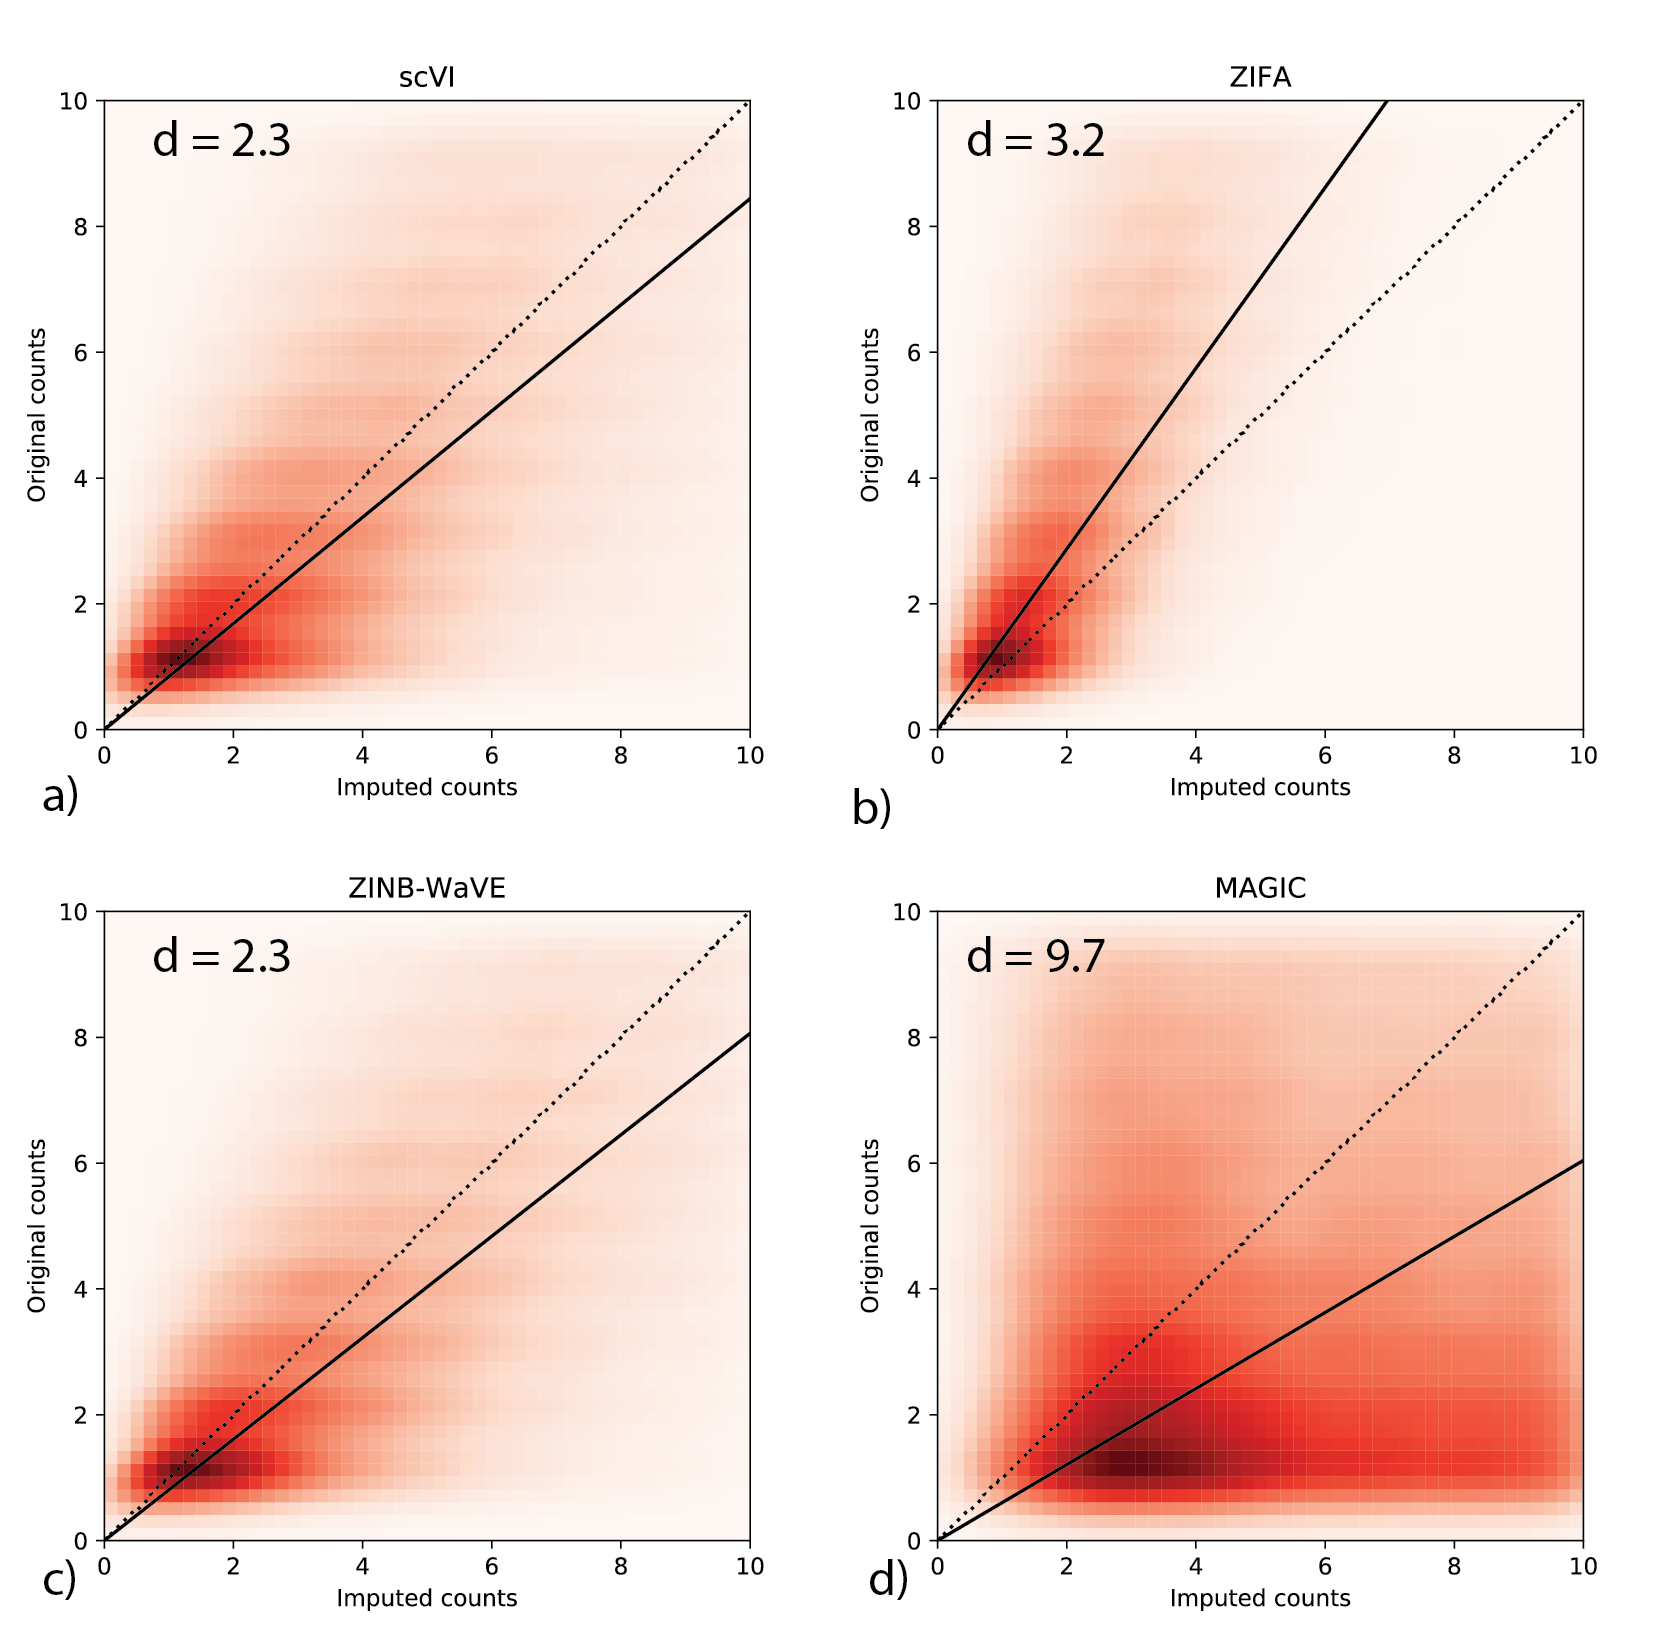
\includegraphics[width=\textwidth]{figures/Figure-3.png}
\caption[Imputation of scVI on the CORTEX dataset]{Imputation of scVI on the CORTEX dataset. The heatmaps denote density plots of imputed values (by scVI, ZIFA, MAGIC and ZINB-WaVE respectively) on a down-sampled version versus the original (non- zero) values prior to down-sampling. The reported score $d$ is the median imputation error across all the hidden entries (Lower is better; see Methods).}
\label{scviimpute_panel}
\end{figure}

To provide an example in which the perturbed values depend on the amount of mRNA observed, we also generated a corrupted training set by downsampling $10\%$ uniformly chosen non-zero entries with a binomial law of rate $20\%$. These values guarantee that most of the dataset is unchanged and require that the model has enough flexibility to impute correctly the changed values. With respect to these corruption scheme, scVI also performs well (Figure~\ref{scvilog_imputation_non_unif}, ~\ref{scvilog_imputation_non_unif_supp}).
% for revision, think about regularization on the dispersion parameters as in ZINB-WaVE
% Also, commenting on how imputation get worse with number of genes would help for understanding

scVI, like ZIFA and FA, can also be used to generate unseen data by sampling from the latent space. As evidence of the validity of this procedure, we sampled from the posterior distribution given the perturbed training data and observed that the samples are largely consistent with the unperturbed data (Figure~\ref{scviposterior_supp}).


\subsection{Capturing biological structure in a latent space}
\label{scviclustering_results}
To further assess the performance of scVI, we evaluated how well its latent space summarizes biological information and recovers biologically coherent subpopulations. For these experiments, we used three datasets where pre-annotated clusters or subpopulations are available: CORTEX, PBMC and RETINA. We then examined whether the annotated subpopulations were distinguishable in the latent space, as in \cite{Wang2017}. 

\subsubsection{Annotation-based evaluation metrics}
We report two different type of metrics for this analysis. The first is silhouette width~\cite{ROUSSEEUW198753}, which evaluates whether cells from the same subpopulation have a similar latent representation and cells from different subpopulations have a different representation. The silhouette width requires either a similarity matrix or a latent space. We can define a silhouette score for each sample $i$ with:
\begin{align}
    s(i) = \frac{b(i) - a(i)}{\max\{a(i),b(i)\}}, 
\end{align}
where $a(i)$ is the average distance of $i$ to all data points in the same cluster $c_i$ and $b(i)$ is the lowest average distance of $i$ to all data points in the same cluster $c$ among all clusters $c$. Clusters can be replaced with batches if we are estimating the silhouette width for assessing batch effects~\cite{SCONE}.

For the second metric, we used the latent representation as an input to the $K$-means algorithm (with $T=200$ random initializations to achieve a stable score), and measured the overlap between the resulting clustering annotations and the pre-specified subpopulations using the adjusted rand index (ARI) and normalized mutual information (NMI) scores. For ease of comparison across methods, we set $K$ to the number of annotated subpopulations.

The ARI is defined as:
\begin{align}
    ARI = \frac{\sum_{ij} \binom{n_{ij}}{2} - [\sum_i \binom{a_i}{2} \sum_j \binom{b_j}{2}] / \binom{n}{2} }{ \frac{1}{2} [\sum_i \binom{a_i}{2} + \sum_j \binom{b_j}{2}] - [\sum_i \binom{a_i}{2} \sum_j \binom{b_j}{2}] / \binom{n}{2}},
\end{align}
where $n_{ij}, a_i, b_j$ are values from the contingency table. 

The NMI is defined as 
\begin{align}
NMI = \frac{I(P;T)}{\sqrt{\mathbb{H}(P)\mathbb{H}(T)}}
\end{align}
where $P, T$ designates empirical categorical distributions for the predicted and real clustering. $I$ is the mutual entropy and $\mathbb{H}$ is the Shannon entropy.

\subsubsection{Annotation-agnostic evaluation metrics}
While these annotated subpopulations were subject to manual inspection and interpretation, a remaining caveat is that they are computationally derived. To address this, we make use of the CBMC dataset that includes measurements of thirteen key marker proteins in addition to mRNA. For evaluation, we quantify the extent to which the similarity between cells in the mRNA latent space resembles their similarity at the protein level. To this end, we compute the overlap fold enrichment between the protein and mRNA-based cell 100-nearest neighbor graph and the Spearman correlation of the adjacency matrices.
% For revision, consider running the p values (with tail of hypergeometric distribution)

\subsubsection{Results}

Based on these benchmarks, we compared scVI to other methods that aim to infer a biologically meaningful latent space (ZIFA, ZINB-WaVE, DCA, and FA), using the same clustering scheme. We find that scVI compares favorably to these methods for all of the datasets (Figure~\ref{scviclustering_supp}ab). Focusing on the PBMC dataset, we also compared scVI with a simpler version that does not explicitly model library size. Our results (Figure~\ref{scviclustering_supp}a) suggests that this additional modeling increases the clustering abilities of scVI. Next, we benchmark scVI with SIMLR \cite{Wang2017}, a method that couples clustering with learning a cell-cell similarity matrix. For the first set of tests, we set the number of clusters in SIMLR to be the true number of annotated subpopulations. For the CBMC case, we let SIMLR automatically determine that number. When we examine the evaluations that were based on the computationally derived annotations, we find that SIMLR outperforms scVI (Figure~\ref{scviclustering_supp}ab). However, while the latent space inferred by SIMLR provides a tight representation for these subpopulations, it may disregard other forms of critical information. Indeed, in the CBMC-based test, where the clustering is based on ``external'' but biologically meaningful data, scVI and DCA are the best performing methods, albeit by a small margin (Figure~\ref{scviclustering_supp}c).

\begin{figure}
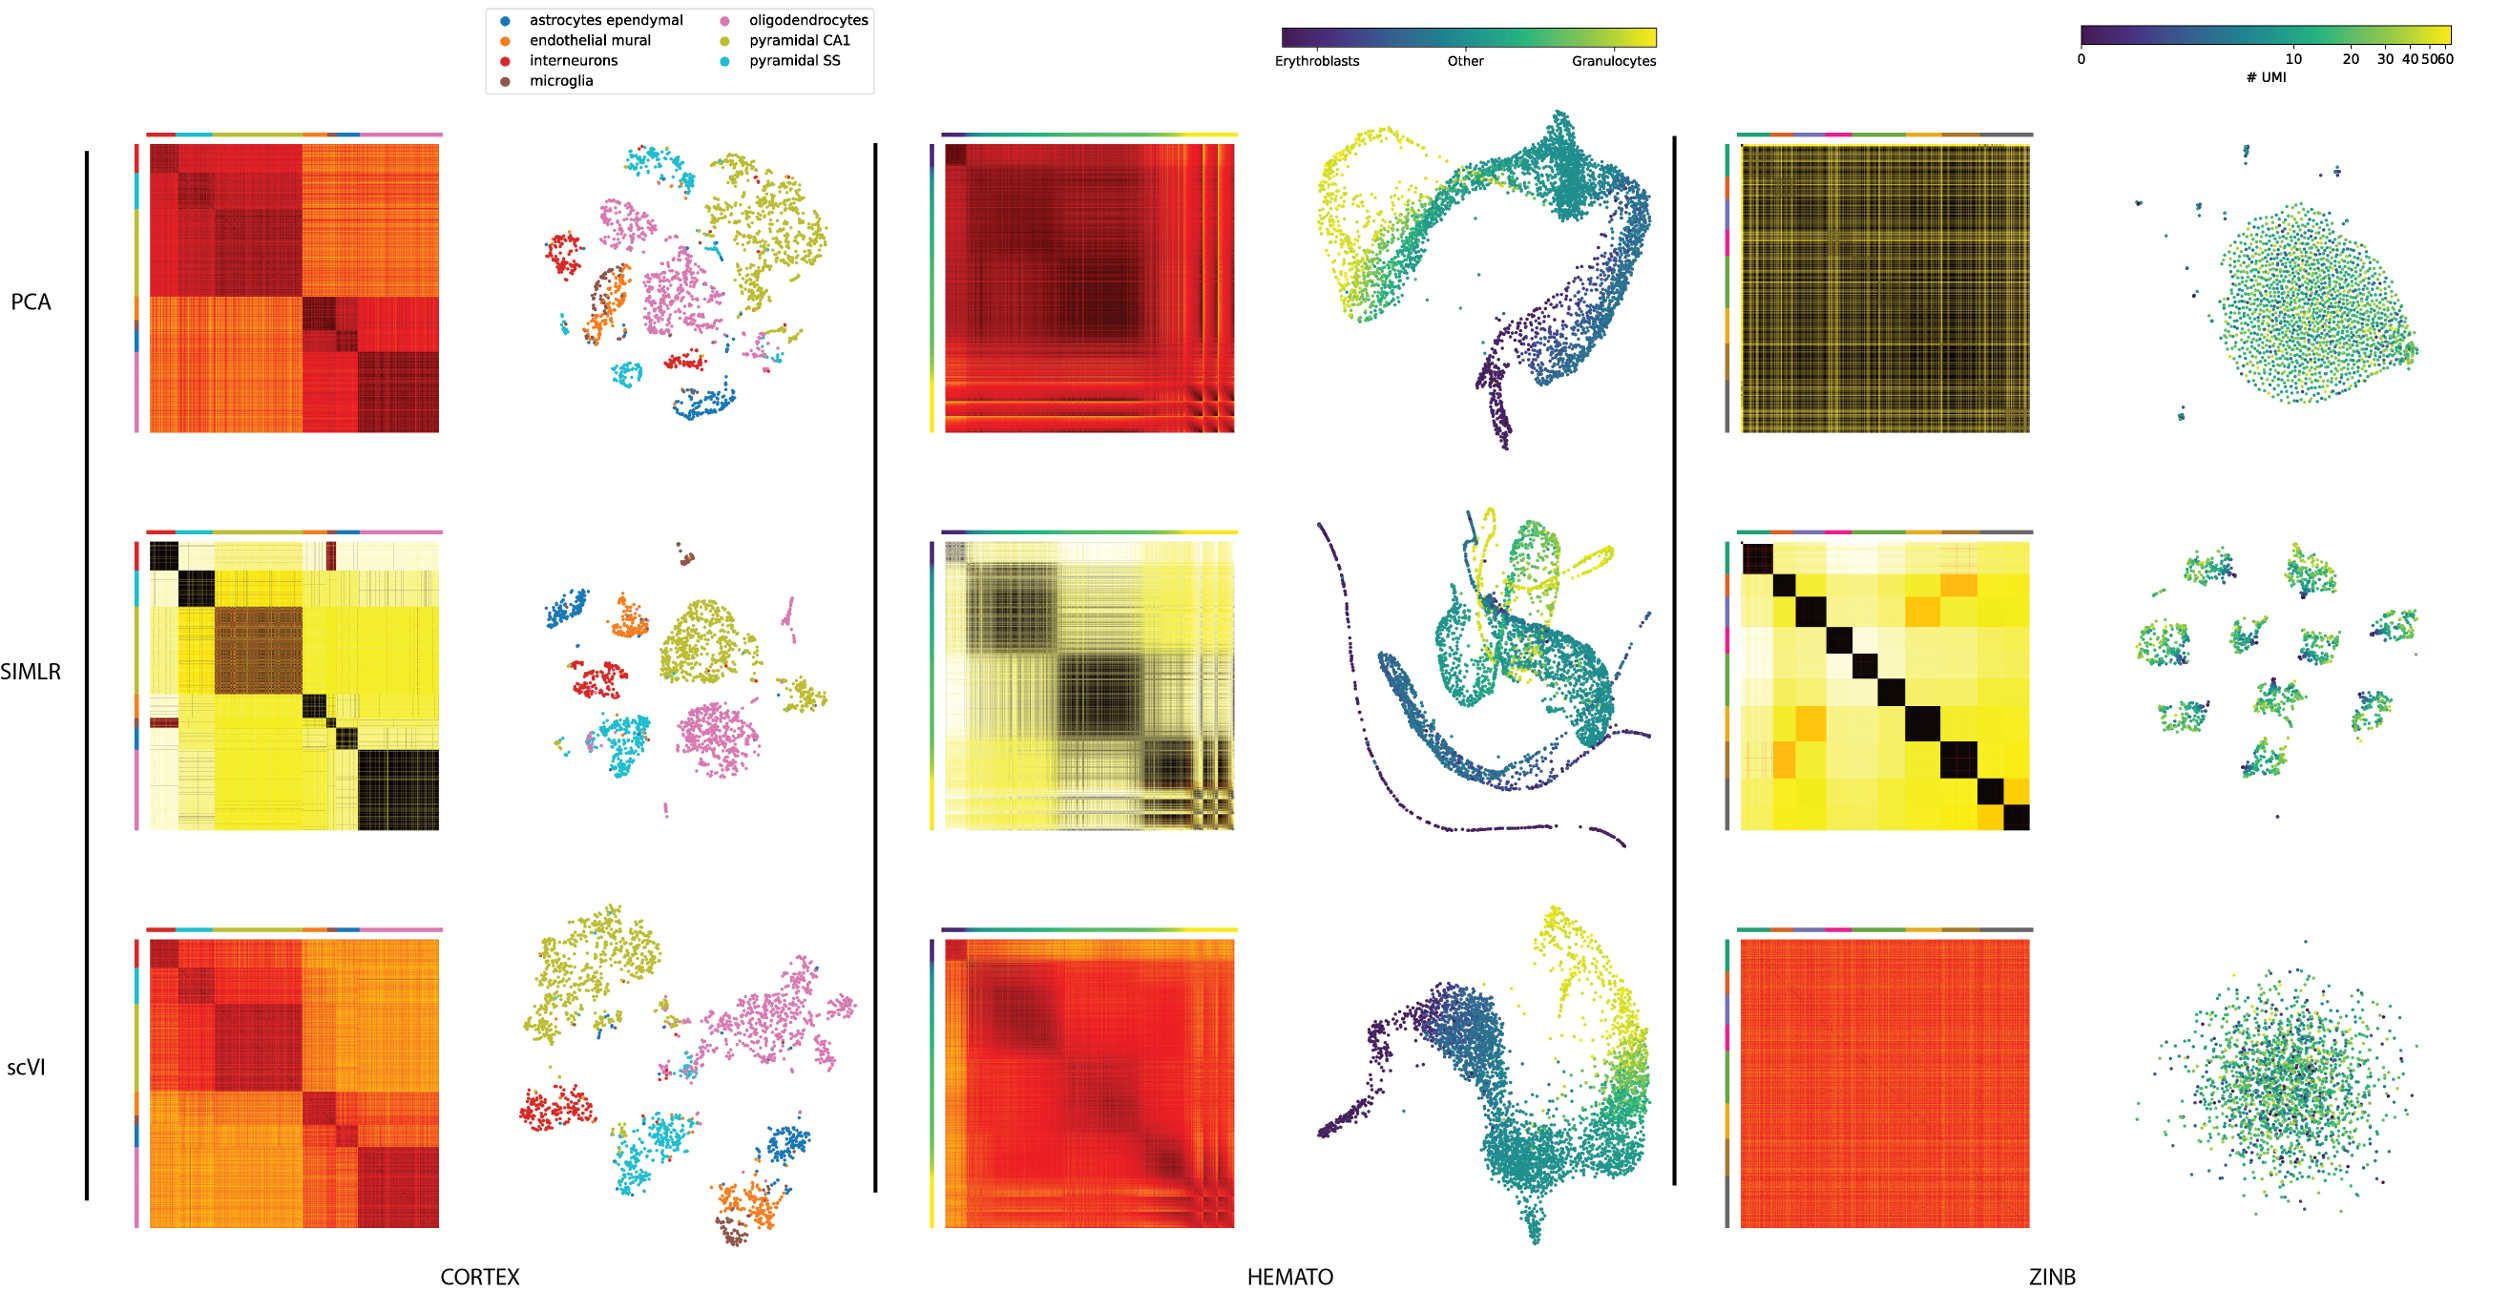
\includegraphics[width=\textwidth]{figures/Figure-2}
\centering
\caption[Clustering panel for scVI, PCA and SIMLR]{We apply scVI, PCA and SIMLR to three datasets (from right to left: CORTEX, HEMATO and a simulated `'noise'' dataset sampled iid from a fixed zero-inflated negative binomial (ZINB) distribution). For each dataset, we show a distance matrix in the latent space, as well as a two-dimensional embedding of the cells. Distance matrices: the scales are in relative units from low to high similarity (over the range of values in the entire matrix). For CORTEX and HEMATO, cells in the matrices are grouped by their pre-annotated labels, provided by the original studies (for the CORTEX dataset, cell subsets were ordered using hierarchical clustering as in the original study). For ZINB, the color in the distance matrices is determined by the clusters found by SIMLR on this data.  Embedding plots: each point represents a cell and the layout is determined either by tSNE (CORTEX, ZINB) or by a 5-nearest neighbors graph visualized using a Fruchterman-Reingold force-directed algorithm (HEMATO; see Figure~\ref{scvisuppfig2}d for the original embedding for SIMLR). For CORTEX and HEMATO, the color scheme in the embeddings is the same as in the distance matrices. For ZINB, the colors reflect the number of UMI in each cell (see Figure~\ref{scvisuppfig2}a-c for coloring of cells according to SIMLR clusters)}
\label{scviclustering_panel}
\end{figure}


Another example of important information that may be missed is the hierarchical structure among clusters, such as the one reported for the CORTEX dataset~\cite{Zeisel1138}. We take several cuts at different depths of the hierarchical clustering (Table~\ref{scvicortex-celltypes}) and report clustering scores based on these agglomerated labels (Figure~\ref{scviclustering_supp}efg). These results suggest that scVI and ZINB-WaVE find low-dimensional representations that better preserve this important biological structure.


A second important case occurs when the variation between cells has a continuous, rather than discrete, form. An example of this is the HEMATO dataset, which consists of hematopoietic cells annotated along seven different stages of differentiation. As a first step, we focus on cell development towards either granulocytic neutrophil or erythoid fate~\cite{Tusi2018}. SIMLR applied to this dataset predicts the presence of five clusters, and the resulting five-nearest-neighbors graph (visualized using a Fruchterman-Reingold force-directed algorithm) does not reflect the continuous nature of this system. Conversely, standard PCA analysis and scVI are able to capture this property of the data (Figure~\ref{scviclustering_panel}), albeit with less precision than the finely tuned process used in the original publication (Figure~\ref{scvihemato_supp}). 

Finally, there may be the case of lack of structure, where the data is almost entirely dominated by noise. To explore this setting, we generated a noise dataset, sampled at random from a vector of zero-inflated negative binomial distributions. SIMLR erroneously reports eleven distinct clusters in this data, which are not perceived by any other method (Figure~\ref{scviclustering_panel},~\ref{scvisuppfig2}a-c).

Altogether, these results suggest that the latent space of scVI is flexible and describes the data well, either as discrete clusters, as a continuum between cell state, or as structureless noise. scVI is therefore better suited than SIMLR in scenarios where the data does not necessarily fit with a simple structure of discrete subpopulations.


\subsection{Controlling for batch effects}
\label{scvibatch_results}
scVI explicitly accounts for the contribution of discrete nuisance factors of variation such as batch annotations in its graphical model. It does so by enforcing conditional independence between them and the inferred parameters.

\begin{figure}[htp]
\centering
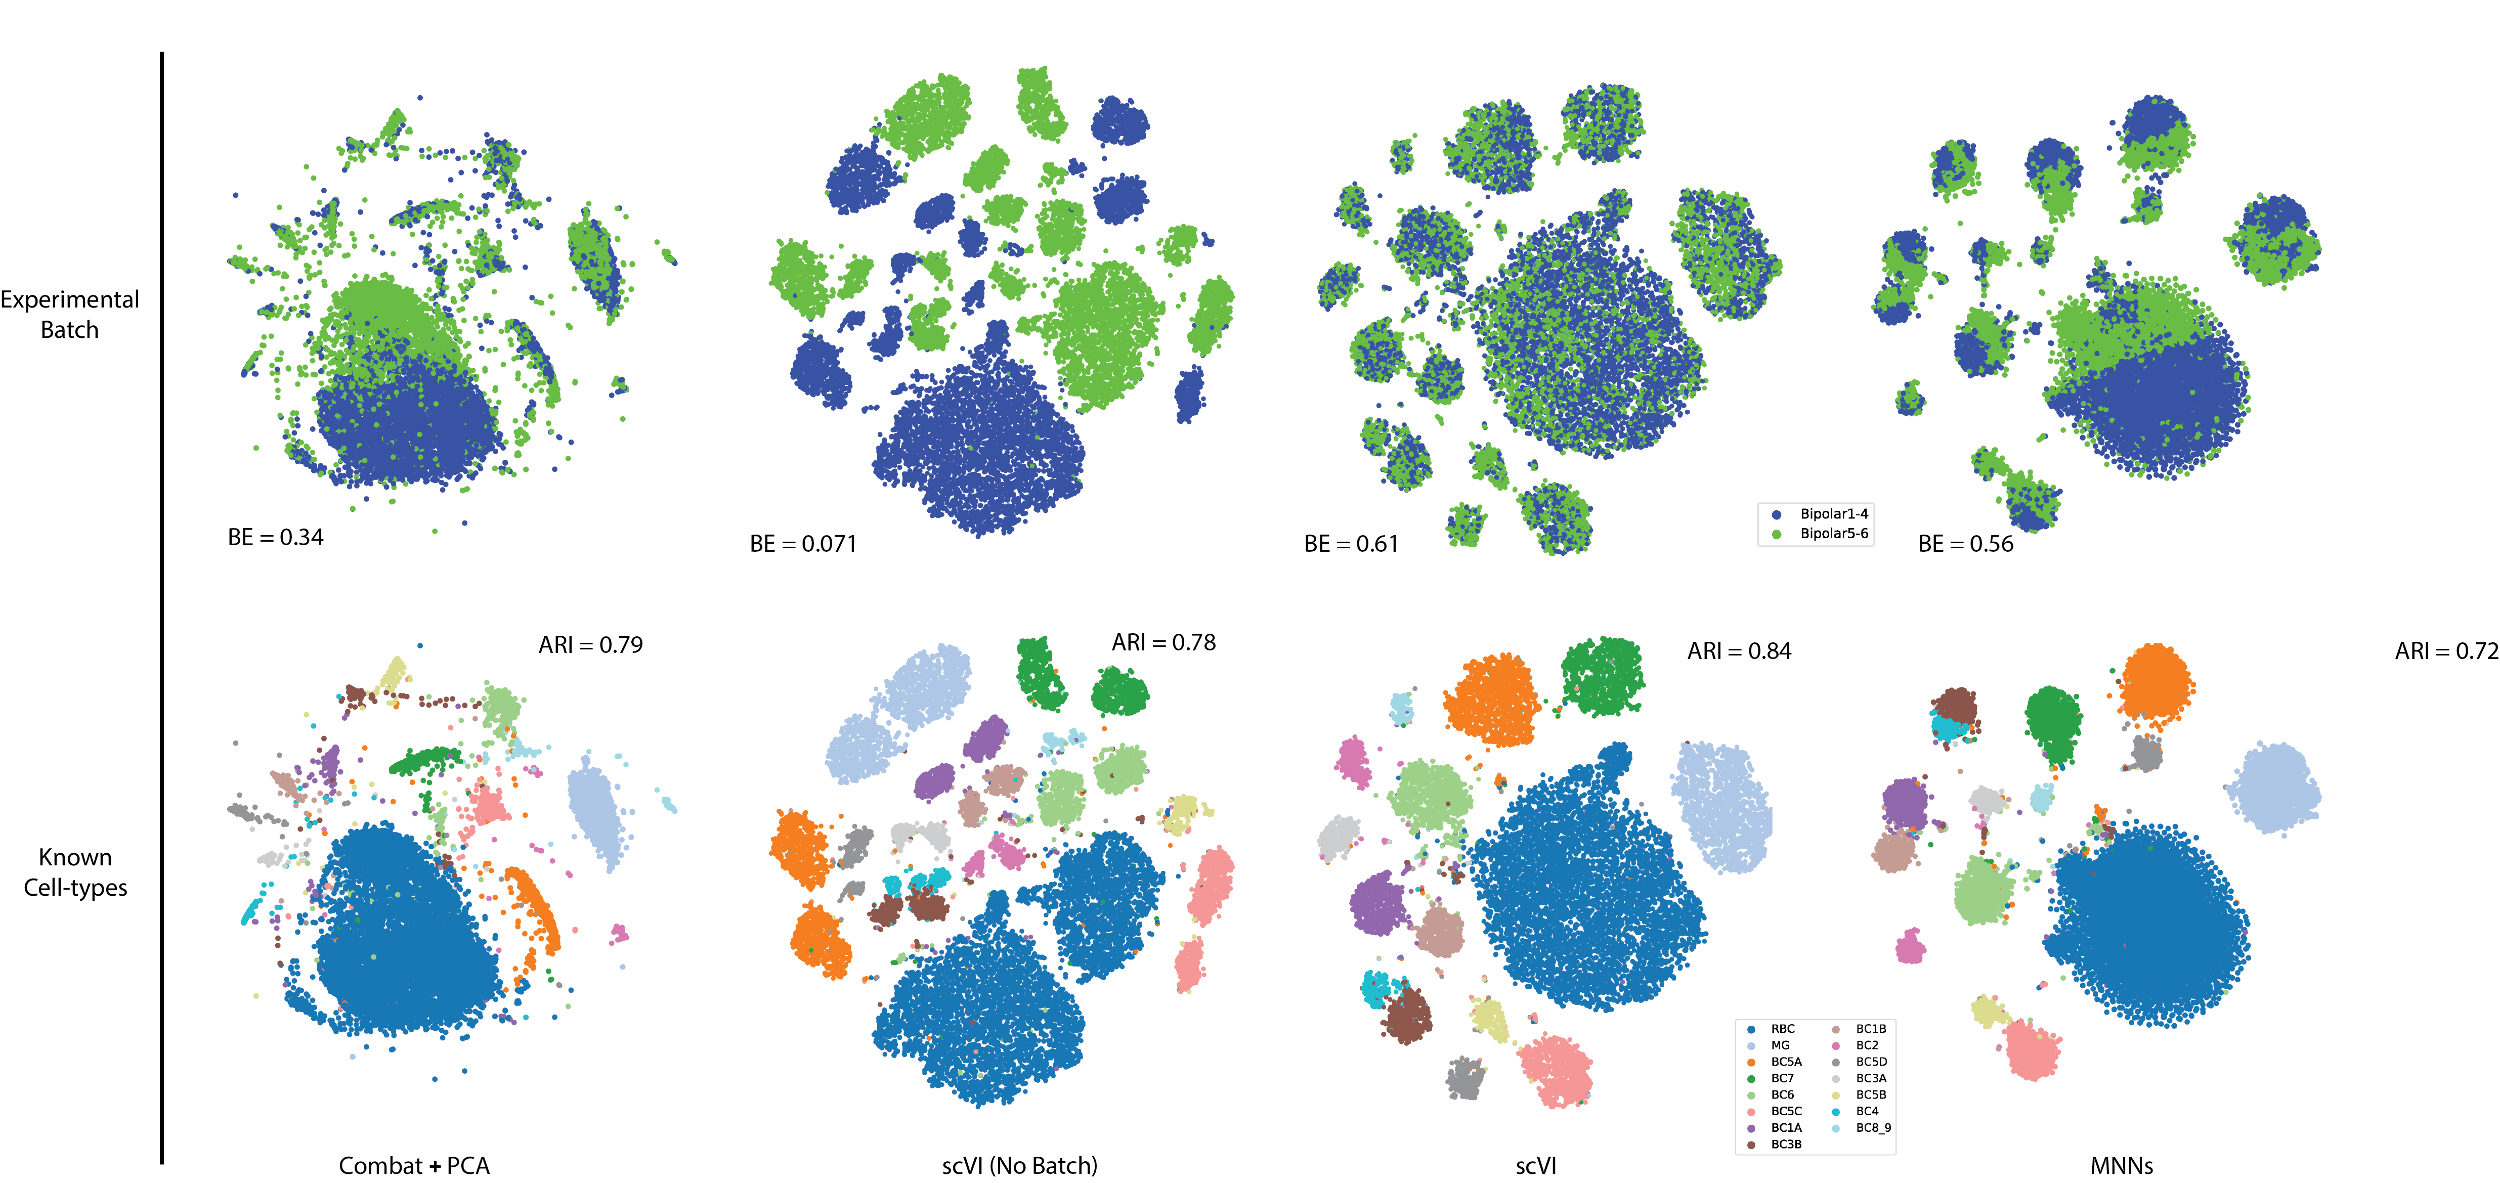
\includegraphics[width=\textwidth]{figures/Figure-5}
\caption[Batch effect removal with scVI on the RETINA dataset]{Batch effect removal with scVI on the RETINA dataset. We visualize the batch removal and clustering performance. A successful method renders a latent space which maintains a satisfactory level of clustering while sufficiently mixing the batches. Embedding plots (PCA with ComBat, scVI without batch correction, scVI and PCA with MNNs) were generated by applying tSNE on the respective latent space. In the upper part of the figure, the cells are colored by batch. In the lower part, cells are colored by the annotation of subpopulations, provided in the original study~\cite{bipolar}. For each algorithm, we report the batch entropy mixing for the batches (BE; higher is better) and the adjusted Rand index for the clustering (ARI; higher is better). When using PCA, we used the top 100 principal components (the top 10 resulted in no discernible structure).}
\label{scvibatch_panel}
\end{figure}

Our model therefore learns gene expression bias that comes from the batch effects and provides a parametric distribution that is disentangled from these technical effects, thus ideally reflecting the relevant biological variation. We evaluate the performance of scVI in correcting for batch effects using the RETINA dataset, which consists of two batches. We measured the entropy of batch mixing across the $K$-nearest neighbors graph with the ideal expectation of a uniform representation of batches (i.e., maximum entropy) in any local neighborhood. We also measure the average silhouette width; with no batch bias, batches should overlap perfectly and exhibit a null silhouette width. We compare our method to the more standard pipeline of batch correction ComBat~\cite{Johnson2007} followed by principal component analysis and the recent mutual nearest neighbors method (MNN~\cite{MNNpaper}). We also report results for methods that do not include batch correction in their underlying model, namely PCA, SIMLR, DCA and a simplified version of scVI with no conditioning for batches (Methods). Our results (Figure~\ref{scvibatch_panel},~\ref{scviclustering_supp}d,~\ref{scviMNNfigure}) demonstrate that in this dataset scVI aligns the batches better than Combat and MNN, while still maintaining a tight representation of pre-annotated subpopulations and compares favorably to all the other algorithms. Considering the latent space provided by algorithms without explicit batch modeling we find, as expected, that the mixing of the batches is poor. Specifically, while SIMLR and DCA are capable of clustering the cells well within each batch, the respective clusters from each batch remain largely separated. Furthermore, the poor batch mixing of the simplified scVI version demonstrates that the additional modeling complexity brought by the batch correction is important. Notably, we performed a similar analysis with the PBMC dataset, which consists of cells from two donors. However, this data seemed to exhibit only a minor batch effect to begin with (our metrics are averaged across all cell-types) and was thus less informative for the purpose of this evaluation  (Figure~\ref{scviclustering_supp}a).


\subsection{Differential expression}
\label{scvide_results}
Identifying genes that are differentially expressed between two subpopulations of cells is an important application of our generative model. The Bayesian model in scVI makes hypothesis testing straightforward. 

\subsubsection{A Bayesian hypothesis testing procedure for scVI}
For each gene $g$ and pair of cells ($z_a$, $z_b$) with observed gene expression $(x_a, x_b)$ and batch ID $(s_a, s_b)$, we can formulate two mutually exclusive hypotheses:
\begin{align}
    \mathcal{M}_1^g:= \mathbb{E}_sf_w^g(z_a, s) > \mathbb{E}_sf_w^g(z_b, s) \textrm{~~~~vs.~~~~} \mathcal{M}_2^g:=\mathbb{E}_sf_w^g(z_a, s) \leq \mathbb{E}_sf_w^g(z_b, s),
\end{align}
where the expectation $\mathbb{E}_s$ is taken with respect to the batch variable empirical frequencies. Notably, we propose a hypothesis testing that do not to calibrate the data to one batch but will find genes that are consistently differentially expressed. 
Again, evaluating the likelihood ratio test for whether our datapoints $(x_a, x_b)$ are more probable under the first hypothesis is equivalent to writing a Bayes factor~\cite{doi:10.1146/annurev-statistics-031017-100307}:
\begin{align}
K = \log_e \frac{p(\mathcal{M}_1^g \mid x_a, x_b)}{p(\mathcal{M}_2^g \mid x_a, x_b)}.
\end{align}
A Bayes factor is a Bayesian generalization of the p-value. Its sign indicates which of $\mathcal{H}_1^g$ and $\mathcal{H}_2^g$ is more likely. Its magnitude is a significance level and throughout the chapter, we consider a Bayes factor as strong evidence in favor of a hypothesis if $|K| > 3$~\cite{Kass1995} (equivalent to an odds ratio of $exp(3)\approx 20$).

The posterior of these models can be approximated by integrating against the variational distribution:
\begin{align}
p(\mathcal{M}_1^g \mid x_a, x_b) \approx \sum_s\iint_{z_a, z_b} p(f_w^g(z_x, s) \leq f_w^g(z_x, s) )p(s)dq(z_a \mid x_a)dq(z_b \mid x_b).
\end{align}
Here $p(s)$ designates the relative abundance of cells in batch $s$ and all of the measures are low-dimensional, so we can use naive Monte Carlo to compute these integrals. We can then use a Bayes factor for the test.

Since we assume that the cells are i.i.d., we can average the Bayes factors across a large set of randomly sampled cell pairs, one from each subpopulation. The average factor will provide an estimate of whether cells from one subpopulation tend to express $g$ at a higher frequency. 


\subsubsection{Benchmarking on real data}
We demonstrate the robustness of our method by repeating the entire evaluation process and comparing the results (Figure~\ref{scvibayes_panel}ab). We also ensure that our Bayes factor are well calibrated by running the differential expression analysis across cells from the same cluster and making sure no genes reach the significance threshold (Figure~\ref{scvibayes_supp}e).

To evaluate scVI as a tool for differential expression, we used the PBMC dataset along with its classification of cells into well-studied subtypes of hematopoietic cells, for which reference bulk expression data is available. 

\begin{figure}
    \centering
    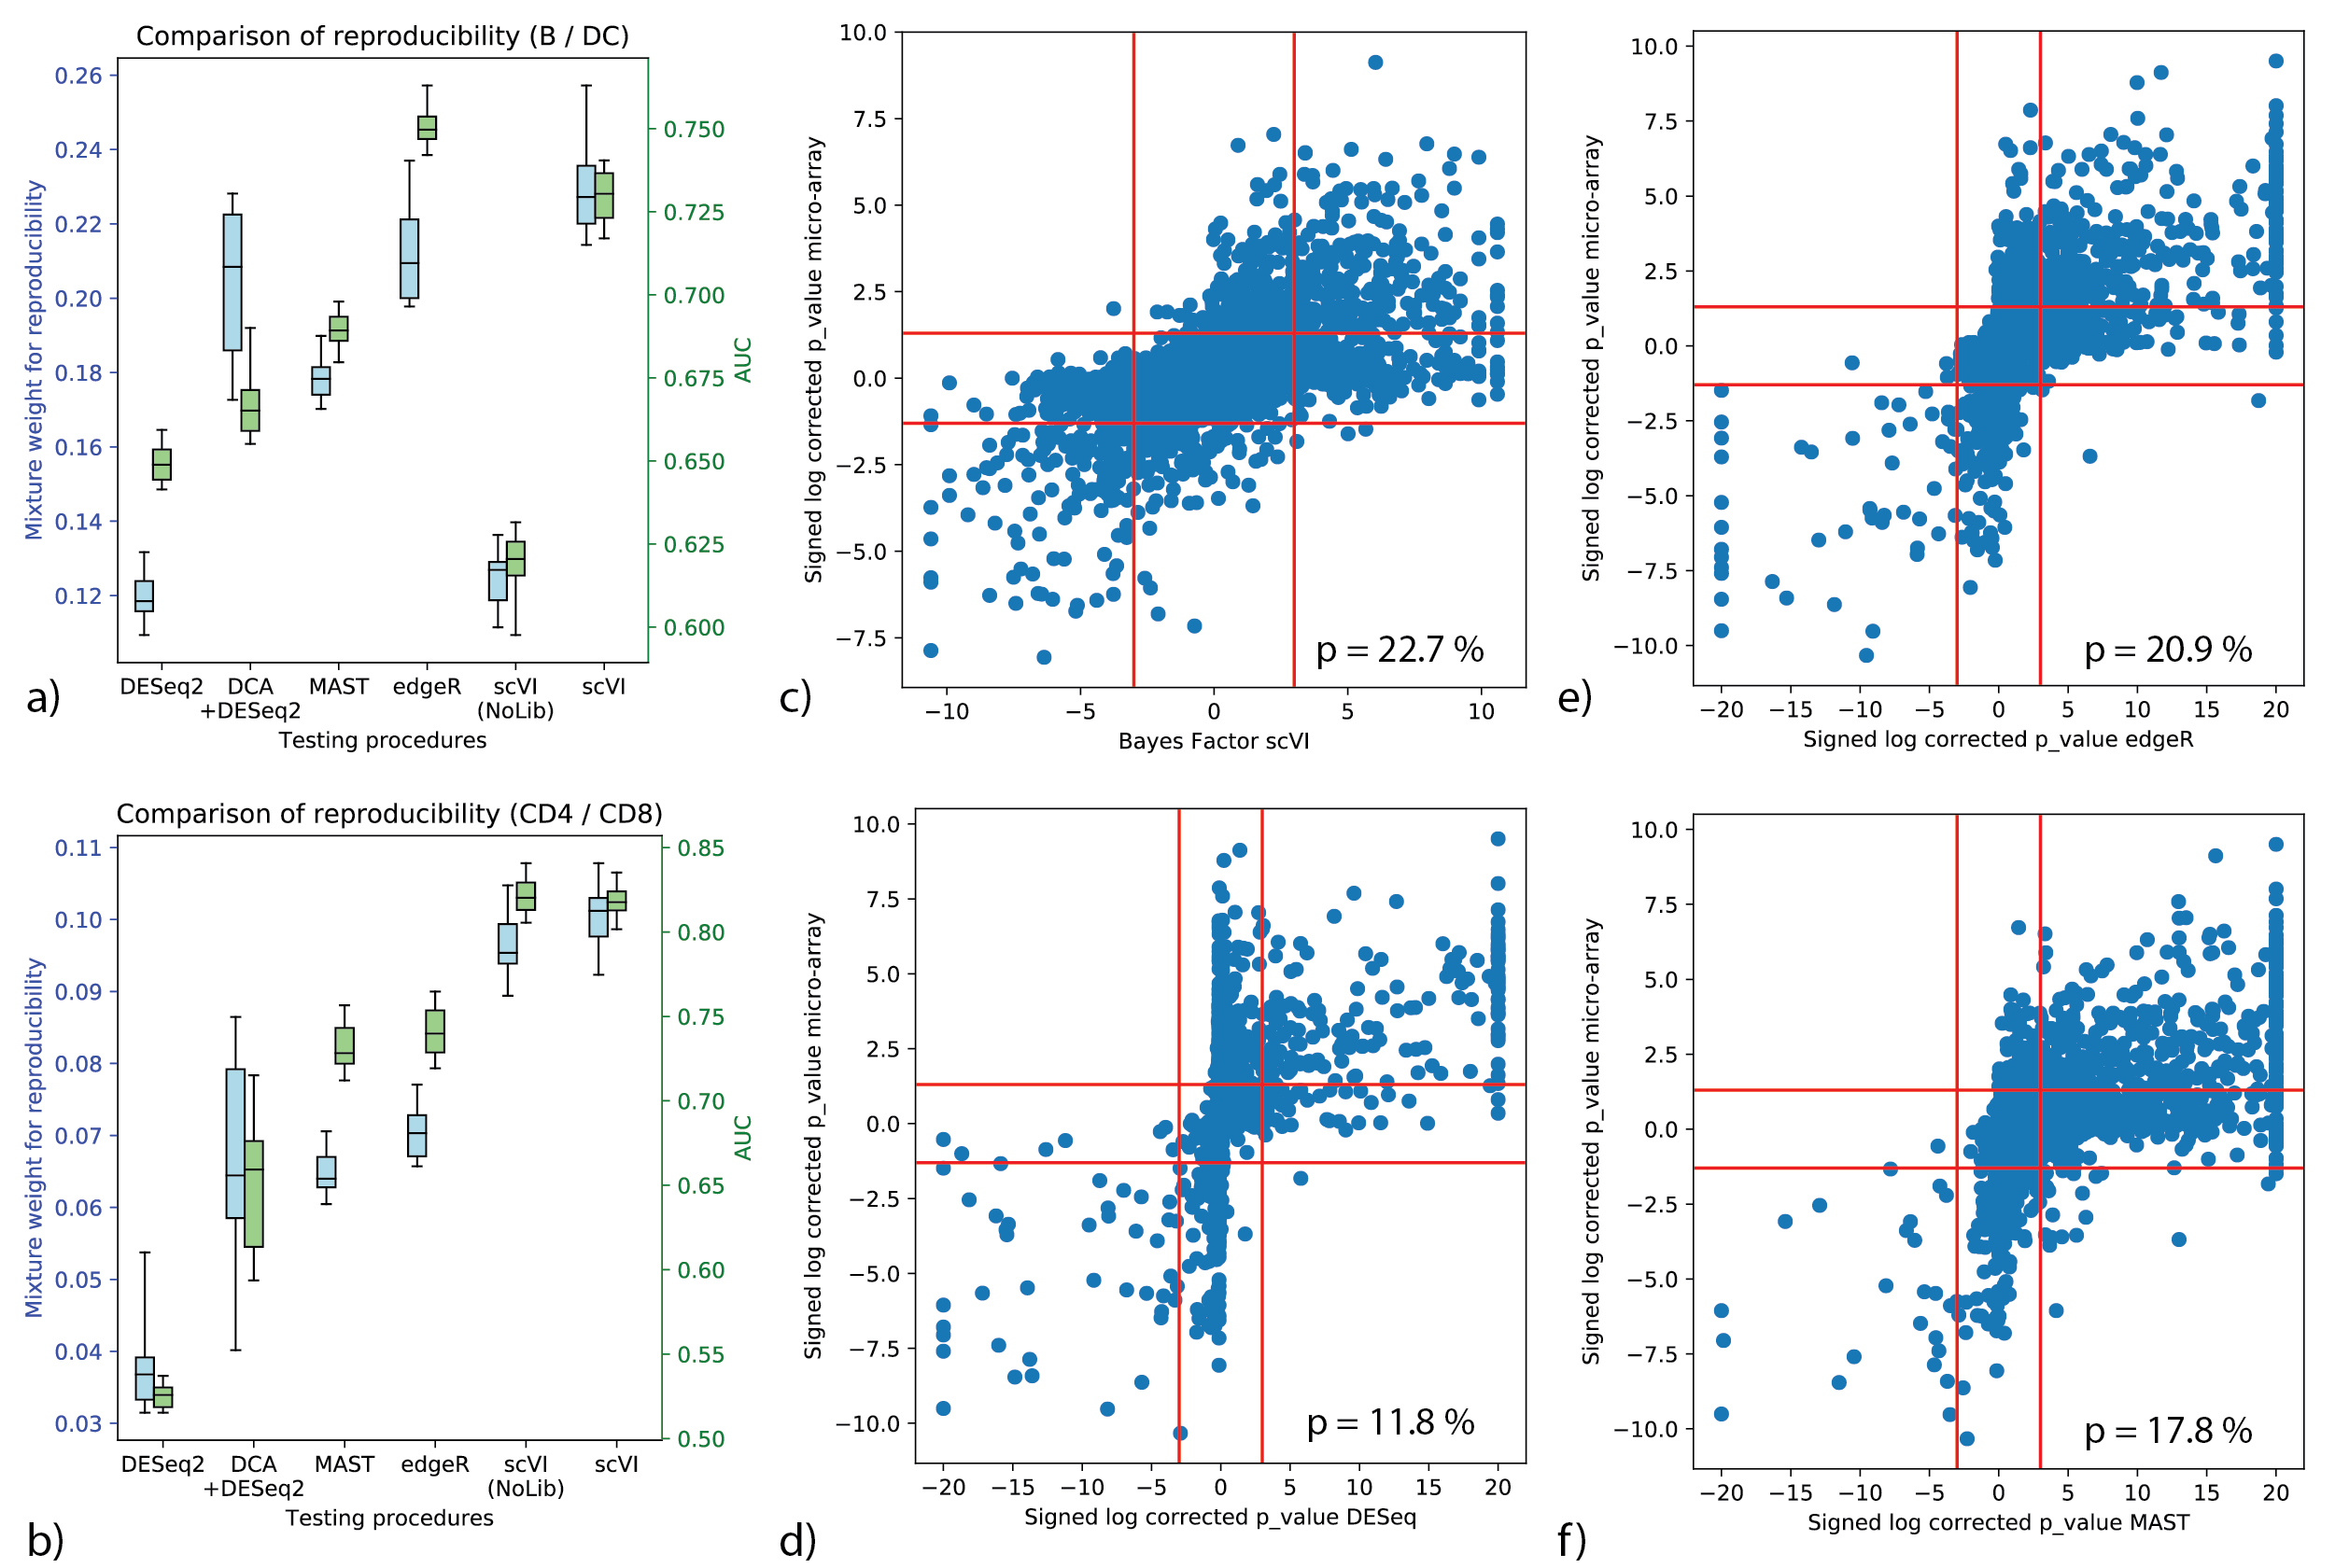
\includegraphics[width=\textwidth]{figures/Figure-4.png}
    \caption[Benchmark of differential expression analysis using the PBMC dataset]{Benchmark of differential expression analysis using the PBMC dataset, based on consistency with published bulk data. (a, b) Evaluation of consistency with the irreproducible discovery rate (IDR)~\cite{Li2011} framework (blue) and using AUROC (green) is shown for comparisons of B cells vs Dendritic cells (a) and CD4 vs CD8 T cells (b). Error bars are obtained by repeatedly sub-sampling the data to show robustness. Whiskers denote the 5th and 95th percentiles.  (c,d,e,f): correlation of significance levels of differential expression of B cells vs Dendritic cells, comparing bulk data and single cell. Points are individual genes. Bayes factors or p-values on scRNA-seq data are presented on the x-axis; microarray-based  p-values are depicted on the y-axis. Horizontal bars denote significance threshold of 0.05 for corrected p-values. Vertical bars denote significance threshold for the Bayes factor of scVI (c) or 0.05 for corrected p-values for DESeq2 (d), edgeR (e), and MAST (f). We also report the median mixture weight for reproducibility $p$ (higher is better).}
    \label{scvibayes_panel}
    \end{figure}

We compare scVI to three widely used methods: DESeq2~\cite{deseq2}, MAST~\cite{mast} and edgeR~\cite{edgeR}. We also compare scVI to a simpler version of the model in which we do not explicitly model library size. Finally, we compare to a hybrid method where the counts are first imputed by DCA and then used for differential expression with DESeq2, as proposed by the authors~\cite{dca}. To facilitate the evaluation, we defined a reference set of differentially expressed genes using publicly available bulk expression datasets. Specifically, we assembled a set of genes that are differentially expressed between human B cells and dendritic cells (microarrays, n=10 in each group~\cite{Nakaya2011}) and between CD4+ and CD8+ T cells (microarrays, n=12 in each group~\cite{Gorgun2005}). We apply all six methods in these two differential expression tasks (using the respective clusters of cells) and evaluate the consistency with the reference data using two scores. For the first score, we assign each gene with a label of DE or non-DE based on their p-values from the reference data (genes with a corrected p-values under $0.05$ are positive and the rest are negative); then these labels to compute AUROC for scVI and each of the benchmark methods.
% we could use the genes from GSE to have a better negative set, or think about a signed p value ranking

Since defining the labels requires a somewhat arbitrary threshold,  we use a second score that evaluates the reproducibility of gene ranking (bulk reference vs. single cell; considering all genes), using the irreproducible discovery rate (IDR)~\cite{Li2011}. Considering the AUROC metric, scVI is the best performing method in the T cell comparison, while edgeR outperforms scVI by a smaller margin in the B vs. dendritic cell comparison. Considering the proportion of genes with reproducible rank as fitted by IDR, scVI is the best performing method in both comparisons (Figure~\ref{scvibayes_panel}, Figure~\ref{scvibayes_supp}a-d). Interestingly, the simpler scVI model shows extremely poor performance on the B vs. dendritic cell comparison, being the only model that does not explicitly handle normalization. This is evidence of the usefulness of explicitly including library size normalization in the scVI model. Furthermore, we see that the hybrid method of DCA followed by DESeq2 constitutes a solid improvement over a direct application of DESeq2; however, the performance is still lower than other methods. 
%Taken together, these results suggest that combining models without compatible statistical assumptions might result in a loss of statistical power, hence the advantage of performing all the relevant tasks under the same Hierarchical Bayes model. %NIR: I am not sure what you are referring to here. Is this really an issue with the benchmark methods? %ROMAIN: Let us dump that.


\subsection{Capturing technical variability}
\label{scvitechnicalnoise_results}
To further interpret the fitted models, we study the extent to which they capture technical variability. We focus on datasets that were generated by 10x, as they share the same set of cell quality metrics (generated by cell ranger) and can thus provide reproducible insights about the relationship between our parameters and library quality. Additionally, we required our test datasets to have pre-annotated subpopulations, with the assumption that each subpopulation consists primarily of cells of the same type, thus decreasing the extent of biological heterogeneity (e.g., in total mRNA content). The two datasets that fit these requirements, which we report next, are the PBMC and BRAIN-SMALL.

In each case, we trained the model on the entire dataset and then investigated each pre-annotated subpopulation separately. As a general rule, we find that variation in library size correlates strongly with the cell-specific scaling factor, which is to be expected by the definition of the model. Figure~\ref{scvinoise-model}a depicts these results for the CD14+ monocytes subpopulation in the PBMC data (notably, the negative curvature on the plot can be explained by shrinking the values towards the mean due to the use of a prior). Another important nuisance factor to be considered is the limitation in sensitivity, which exacerbates the number of zero entries. In principle, zero entries can be captured by two different components of our model: the negative binomial and the \enquote{inflation} of zeros added to it with a Bernoulli distribution. Evidently, the expected number of zeros generated by the negative binomial for each cell correlates strongly with the library size and its proxies (e.g., the number of detected genes or the number of reads per UMI; Figure~\ref{scvinoise-model}cd,~\ref{scviparameters_supp}d). This result can be explained by our definition of the negative binomial mean, which is the predicted frequency of expression $\rho_n^g$ scaled by the respective library size $\ell_n$.

The remaining question is therefore, what is the relationship between the expected frequency of expression $\rho_n^g$ and the observed zeros? A simple model would consist of a random process of sampling genes from each cell, in a manner proportional to their frequency, and with no added bias (e.g., in capture efficiency). To explore this, for every gene we plot the mean expected frequency against the percent of detecting cells in a subpopulation of interest (Figure~\ref{scvinoise-model}b). The resulting trend supports this simple model as it closely fits with the zero probability of a hypergeometric distribution---namely, random sampling of molecules without replacement.

Interestingly, the number of additional zeros induced by the Bernoulli random variable in each cell is less correlated with library size, and instead correlates with metrics of alignment rate (Figure~\ref{scvinoise-model}cd,~\ref{scviparameters_supp}cd). These metrics are not necessarily coupled to size, but may reflect other technical factors such as contamination or the presence of degraded mRNA. However, we observed that most zero values in the data can be explained by the negative binomial component alone (Figure~\ref{scviparameters_supp}a). Taken together, these results therefore corroborate the idea that most zeros, at least in the datasets explored here, can be explained by low (or zero) ``biological'' abundance of the respective transcript, which is exacerbated by limited sampling. 


\begin{figure}
\centering
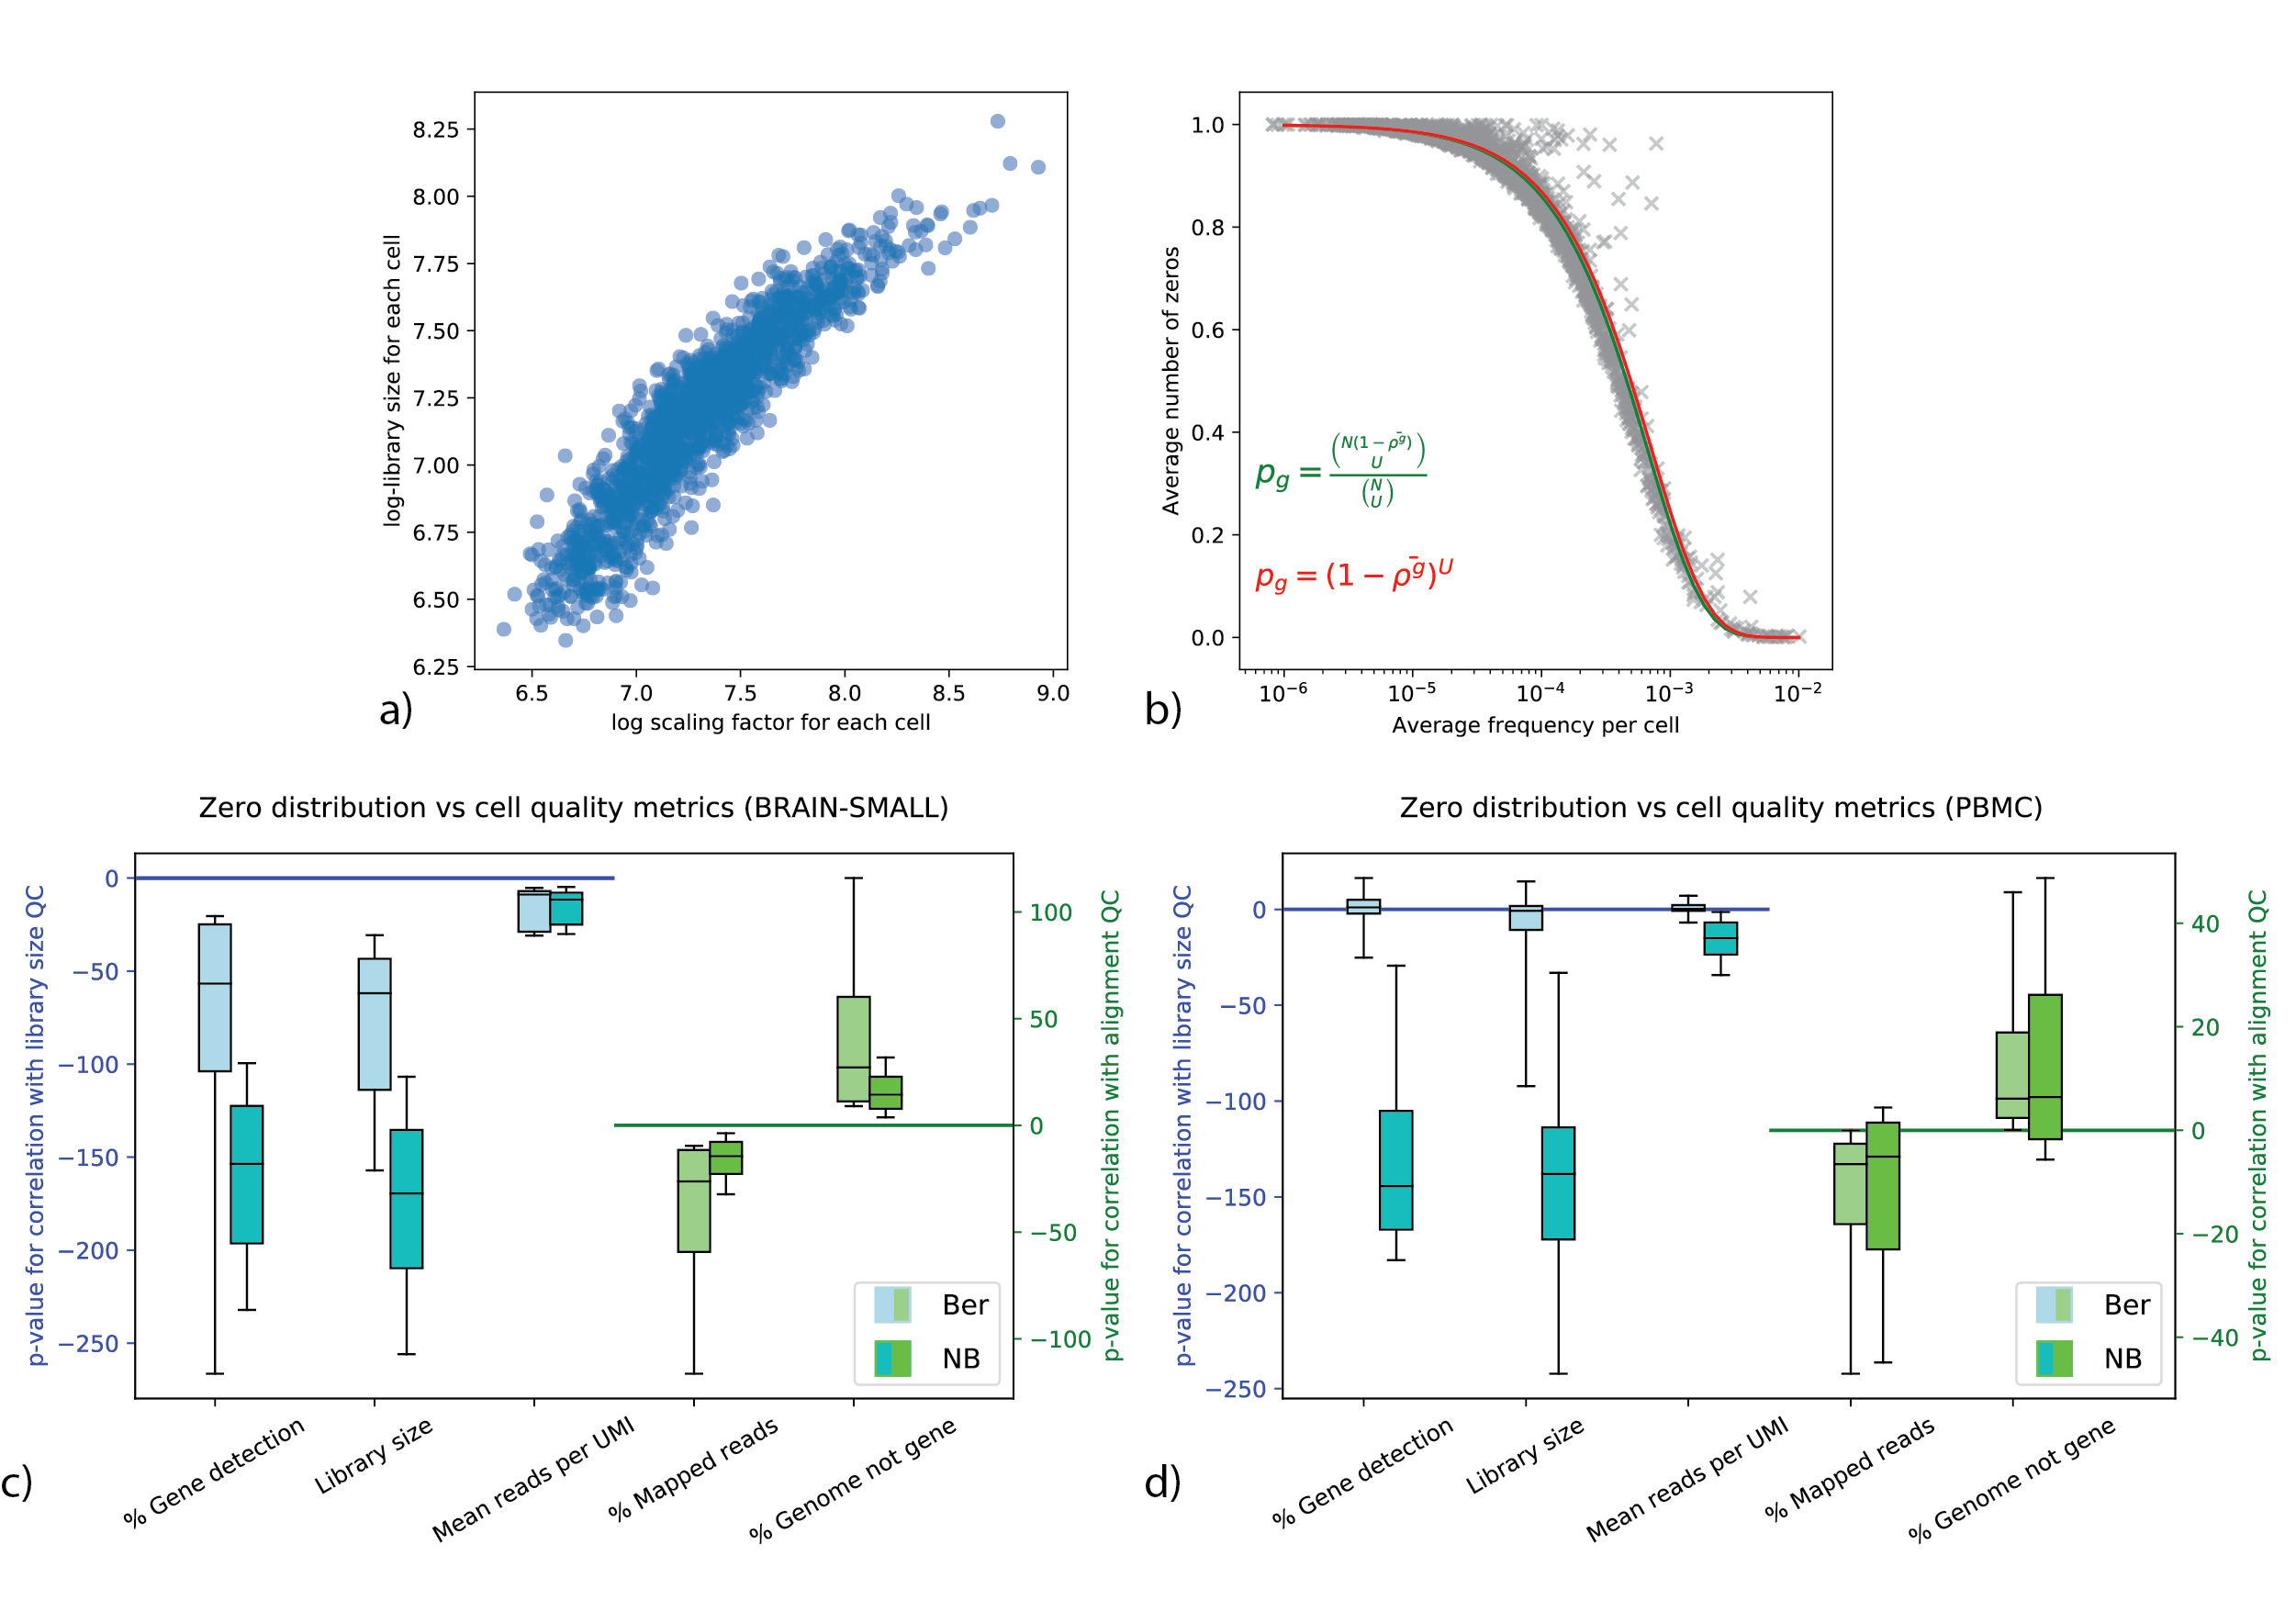
\includegraphics[width=0.95\textwidth]{figures/Figure-6.png}
\caption[Capturing technical variability using scVI]{Capturing technical variability using scVI. Data for panels a-b is based on the CD14+ cell subpopulation of the PBMC dataset. (a) Scatter plot for each cell of inferred scaling factor using scVI against library size. 
% Change the axis
(b) The frequency of observed zero values versus the expected expression level, as produced by scVI. Each point represents a gene $g$, where the x-axis is $\bar{\rho^g}$---the average expected frequency per cell (for gene $g$, average over $\rho_c^g$ for all cells $c$ in the subpopulation), and the y-axis the is observed percentage of cells that detect the fee (UMI>0). The green curve depicts the probability for selecting zero transcripts from every gene as a function of its frequency, assuming a simple model of sampling $U$ molecules from a cell with $N$ molecules at random without replacement. $U=1398$ is the average number of UMIs in the subpopulation and $N$ is the average number of transcripts per cell (for this curve $N=10k$). Notably, the curve converges for values larger than $20k$ to the red curve, a binomial selection procedure (conform to the probabilistic limit of the sampling process when $N\rightarrow \infty$). (c, d) Signed log p-values for testing correlations between the zero probabilities from the two distributions (negative binomial, Bernoulli) and quality control metrics across five random initializations of scVI and all subpopulations of the PBMC and BRAIN-SMALL datasets. Whiskers denote the 5th and 95th percentiles.}
\label{scvinoise-model}
\end{figure}


\subsection{Alternative modeling choices}
We consider here the extent to which each of a sequence of modeling choices in the design of scVI contributes to its performance. As a baseline approach, consider normalizing single-cell RNA sequencing data as in previous literature~\cite{zifa} and reducing the dimensionality of the data using a variational autoencoder with a Gaussian prior and a Gaussian conditional probability. 
    
One way in which a model can be enhanced is by changing the Gaussian conditional probability to one of the many available count distributions, such as zero-inflated negative binomial (ZINB), negative binomial (NB), Poisson or others. Recent work by Eraslan and colleagues using simulated data shows that when the dropout effect drives the signal-to-noise ratio to a less favorable regime, a denoising autoencoder with mean squared error (i.e., Gaussian conditional likelihood) cannot recover cell-types from expression data while an autoencoder with ZINB conditional likelihood can~\cite{dca}. This results points to the importance of at least modeling the sparsity of the data and is consistent with previous contributions~\cite{zifa,zinbwave}. 
    
The next question is which count distribution to use. In scVI we have chosen to use the zero-inflated negative binomial, a choice motivated by previous literature (e.g.,~\cite{zinbwave}). First, the choice of negative binomial is common in RNA-sequencing data, as it is over dispersed~\cite{deseq2}. Furthermore, under some assumption this distribution captures the steady state form of the canonical two-state promoter activation model~\cite{Grun2014}. Finally, recent work by Gr{\o}nbech and colleagues~\cite{scVAE} proposes an analysis based on Bayesian model selection (held-out log-likelihood as in this manuscript). In that analysis, the NB and ZINB distribution stand out with similarly high scores. We demonstrate that the addition of a zero-inflation (Bernoulli) component is important for explaining a subset of the zero values in the data (Figure~\ref{scviparameters_supp}) and that it captures important aspects of technical variability which are not captured by the NB component (Figure~\ref{scvinoise-model}).
    
To enhance the model further, we added terms to account for library-size as a nuisance factor, which can be considered as a Bayesian approach to normalization as in~\cite{biscuit,basics}. We showed how this contributes to our model by increasing clustering scores and the accuracy of differential expression analysis.
    
As a further enhancement, we designed the generative model to explain data from different experimental batches. This is not a trivial task as there may exist a significant covariate shift between the observed transcript measurements. We also showed how this modification to our model is crucial when dealing with batch effects.
\section{Discussion}

% intro
Our study focuses on an important need in the field of single-cell RNA-seq -- namely, a method capable of accounting for confounding factors and measurement uncertainty in tertiary analysis tasks (e.g., clustering, differential expression, and annotation) through a common, scalable statistical model. To achieve this, we developed scVI -- a hierarchical Bayesian model that makes use of neural networks to provide a complete probabilistic representation of single-cell transcriptomes. In this study, we demonstrated that scVI provides a computationally efficient and ``all-inclusive'' approach to denoising and analyzing gene expression data, and showcased its performance by comparing it to the state-of-the-art methods for a range of downstream tasks, including dimensionality reduction, imputation, visualization, batch-effect removal, clustering and differential expression.  

The scVI procedure takes as input a matrix of counts, and therefore does not need a preliminary normalization step. Instead, it learns a cell-specific scaling factor as a hidden variable of the model, with the objective of maximizing the likelihood of the data (as in~\cite{biscuit,zinbwave,basics}), which is more justifiable than \emph{a posteriori} correction of the observed counts~\cite{vallejos2017normalizing}. Further, scVI explicitly accounts for the contribution of discrete nuisance factors, such as batch annotations, by enforcing conditional independence between them and the (inferred) parameters that govern gene expression distributions. We demonstrate that these normalization components are needed to achieve good performance in critical tasks such as clustering and differential expression (Figures \ref{scvibatch_panel}, \ref{scvibayes_panel}, \ref{scviclustering_supp}, and \ref{scviMNNfigure}). Notably, the batch correction step is performed via the mild modeling assumption of conditional independence, and therefore scVI is expected to reasonably integrate and harmonize multiple datasets. Further modeling would be needed for more intensive usage of batch removal (number of batches/datasets $\geq 20$) and is left as an avenue for future research. 

%NIR: new section. Please read
%The support provided by scVI to a range of important analysis tasks and the inclusion of nuisance factors in the model distinguish it from other recent applications of neural networks for scRNA-seq analysis~\cite{scvis,VASC,dca,scVAE} (Methods section~\ref{scvirelated_work}). For instance, DCA can only address a subset of the tasks addressed by scVI (Table~\ref{scvialgorithms_pres}). Indeed, DCA performs comparably to scVI at the tasks it was designed for, including imputation (Figures S1 and S3), and clustering a single batch (Figure~\ref{scviMNNfigure}). However, this is not the case for differential expression, possibly due to the need of an external model~\cite{deseq2} for that purpose (since DCA does not define a posterior over the inferred parameters; Figure~\ref{scvibayes_panel}). More critically, we find that DCA may fail to align data from different batches (Figure \ref{scviclustering_supp}, and \ref{scviMNNfigure}), demonstrating that explicitly accounting for batch effects is an important distinguishing feature of scVI, especially provided that many scRNA-seq studies consist of multiple batches.

Another important feature of scVI and other methods based on neural networks~\cite{scvis,VASC,dca,scVAE} is their scalability. Indeed, unlike many of the benchmark methods, scVI is capable of efficiently processing the very large datasets of up to a million cells explored in this study~\cite{Regev2017,10x}. To achieve this high level of scalability while ensuring a good fit to the data, we designed an efficient procedure to learn the parameters of our graphical model. Importantly, exact Bayesian inference is in most cases not tractable for these kinds of models. Furthermore, until recently, even variational inference was rarely applied to such models without restrictive ``conditional conjugacy'' properties. To address this, we use a stochastic optimization procedure that samples our approximation of the posterior distribution (as well as random subsamples or ``mini-batches'' of our dataset), allowing us to efficiently perform inference with arbitrary models, including those with conditional distributions specified by neural networks~\cite{kingma2013}.

 

The deep learning architecture used in scVI is built on several canonical building blocks such as rectified linear units, fully-connected layers, dropout~\cite{Srivastava2014}, mini-batch normalization~\cite{Ioffe2015}, deterministic warm up~\cite{Sønderby2016}, and mean-field approximation to the posterior~\cite{kingma2013}. Together, these building blocks provide the means to effectively fit the generative model of scVI and approximate its posterior. However, an important area of research going forward is to explore other, possibly better, architectures~\cite{Zoph} and procedures for parameter and hyper-parameter tuning~\cite{Bergstra2011}, which may in some instances increase the accuracy of the inferred model. Notably, since our procedure has a random component, and since it optimizes a non-convex objective function, it may give alternative results with different initializations. To address this concern, we demonstrate the stability of scVI in terms of its objective function, as well as imputation and clustering (Figure~\ref{scvirobustness}). Another related issue is that, if there are few observations (cells) for each gene, the prior (and the inductive bias of the neural network) may keep us from fitting the data closely. Indeed, in the case of datasets such as HEMATO~\cite{Tusi2018}, where the number of cells is smaller than the number of genes, some procedure to pre-filter the genes may be warranted. Another approach that could help make scVI applicable to smaller data sets (hundreds of cells), which we intend to explore, is utilizing techniques such as Bayesian shrinkage~\cite{deseq2} or regularization and second order optimization with larger mini-batch size / full dataset ~\cite{zinbwave}. We do however show that for a range of datasets of varying sizes, scVI is able to fit the data well  and capture relevant biological diversity between cells.
%and is capable of producing meaningful downstream analysis.
%For review: stability of \rho values

From a system perspective, single-cell RNA-seq analyses paradoxically benefit from the abundance of zero values, as this allows us to store the data in a sparse (rather than dense) matrix format. A sparse matrix with one million cells and ten thousand genes would represent around 7.5 GB, assuming one percent fill. On the other hand, the output of batch- corrected data is not sparse, and is therefore potentially very large (for 1M cells, approximately 75 GB). While it performs batch correction, scVI still provides a compact representation of the complete data, as it requires only the latent space and the specification of the model (overall, it has a memory footprint of less than 1G, assuming 10 latent variables). One obvious drawback of such compressed representation (apart from the potential loss of information) is that gene expression values need to be computed on the fly; however, this can be done very efficiently in a single pass through the generative networks (which requires approximately 10 seconds for generating the $\rho$ matrix for a test dataset of 500k cells and 8k genes, with the same hardware specification used throughout this chapter). This property makes scVI a good baseline for use in interactive visualization tools~\cite{DeTomaso2016, Fan2016, Wolf2018}.

Looking ahead, it is important to note that the model of scVI is very general and therefore provides a proper statistical framework for other forms of scRNA-seq analysis that were not explored in this chapter, such as lineage inference~\cite{Semrau2017} or cell-state annotation~\cite{tanay2017scaling,wagner2016revealing}. Further, as the scale and diversity of single-cell RNA-seq increase, we expect that there will be a great demand for tools such as scVI, especially in cases where there is interest in harmonizing datasets in a manner that is scalable and conducive to various forms of downstream analysis~\cite{Regev2017}. Indeed, one subsequent research direction would be to merge multiple datasets from a given tissue to build a generative model with biological annotations of cell-types or phenotypical conditions in a semi-supervised fashion. This would allow researchers to ``query'' the generative model with a new dataset in an online fashion in order to ``retrieve'' previous biological information, which would allow verification of reproducibility across experiments, as well as transfer of cell state annotations between studies.


\newpage
\section{Supplementary figures}


\begin{suppfigure}[htp]
  \centering
  \subfloat{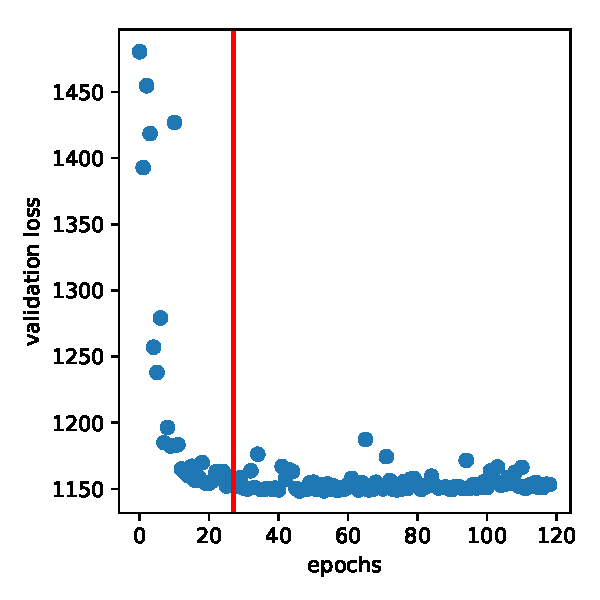
\includegraphics[width=0.49\textwidth]{figures/1M_training_curves.pdf}}
  \hspace{1pt}
  \subfloat{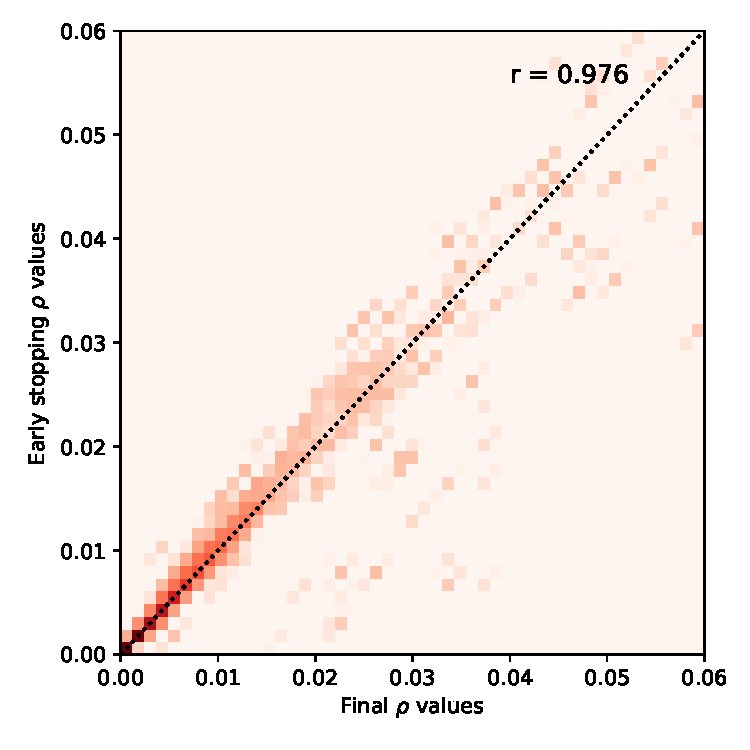
\includegraphics[width=0.49\textwidth]{figures/rho.pdf}}
  \caption[Stability of the early stopping criterion on the one-million-cell sample of the BRAIN-LARGE dataset]{Stability of the early stopping criterion on the one-million-cell sample of the BRAIN-LARGE dataset. (a) Evolution of the loss function ($y$-axis) value on a validation set with the number of epochs ($x$-axis) (b) Contrast of the expected frequency $\rho$-values between the model trained with early stopping ($x$-axis) and the model trained without early stopping ($y$-axis) on a random subset of 100 cells and all genes. We also report the Pearson correlation, $r$.}
\label{scviearly_stopping}
\end{suppfigure}


\begin{suppfigure}[p]
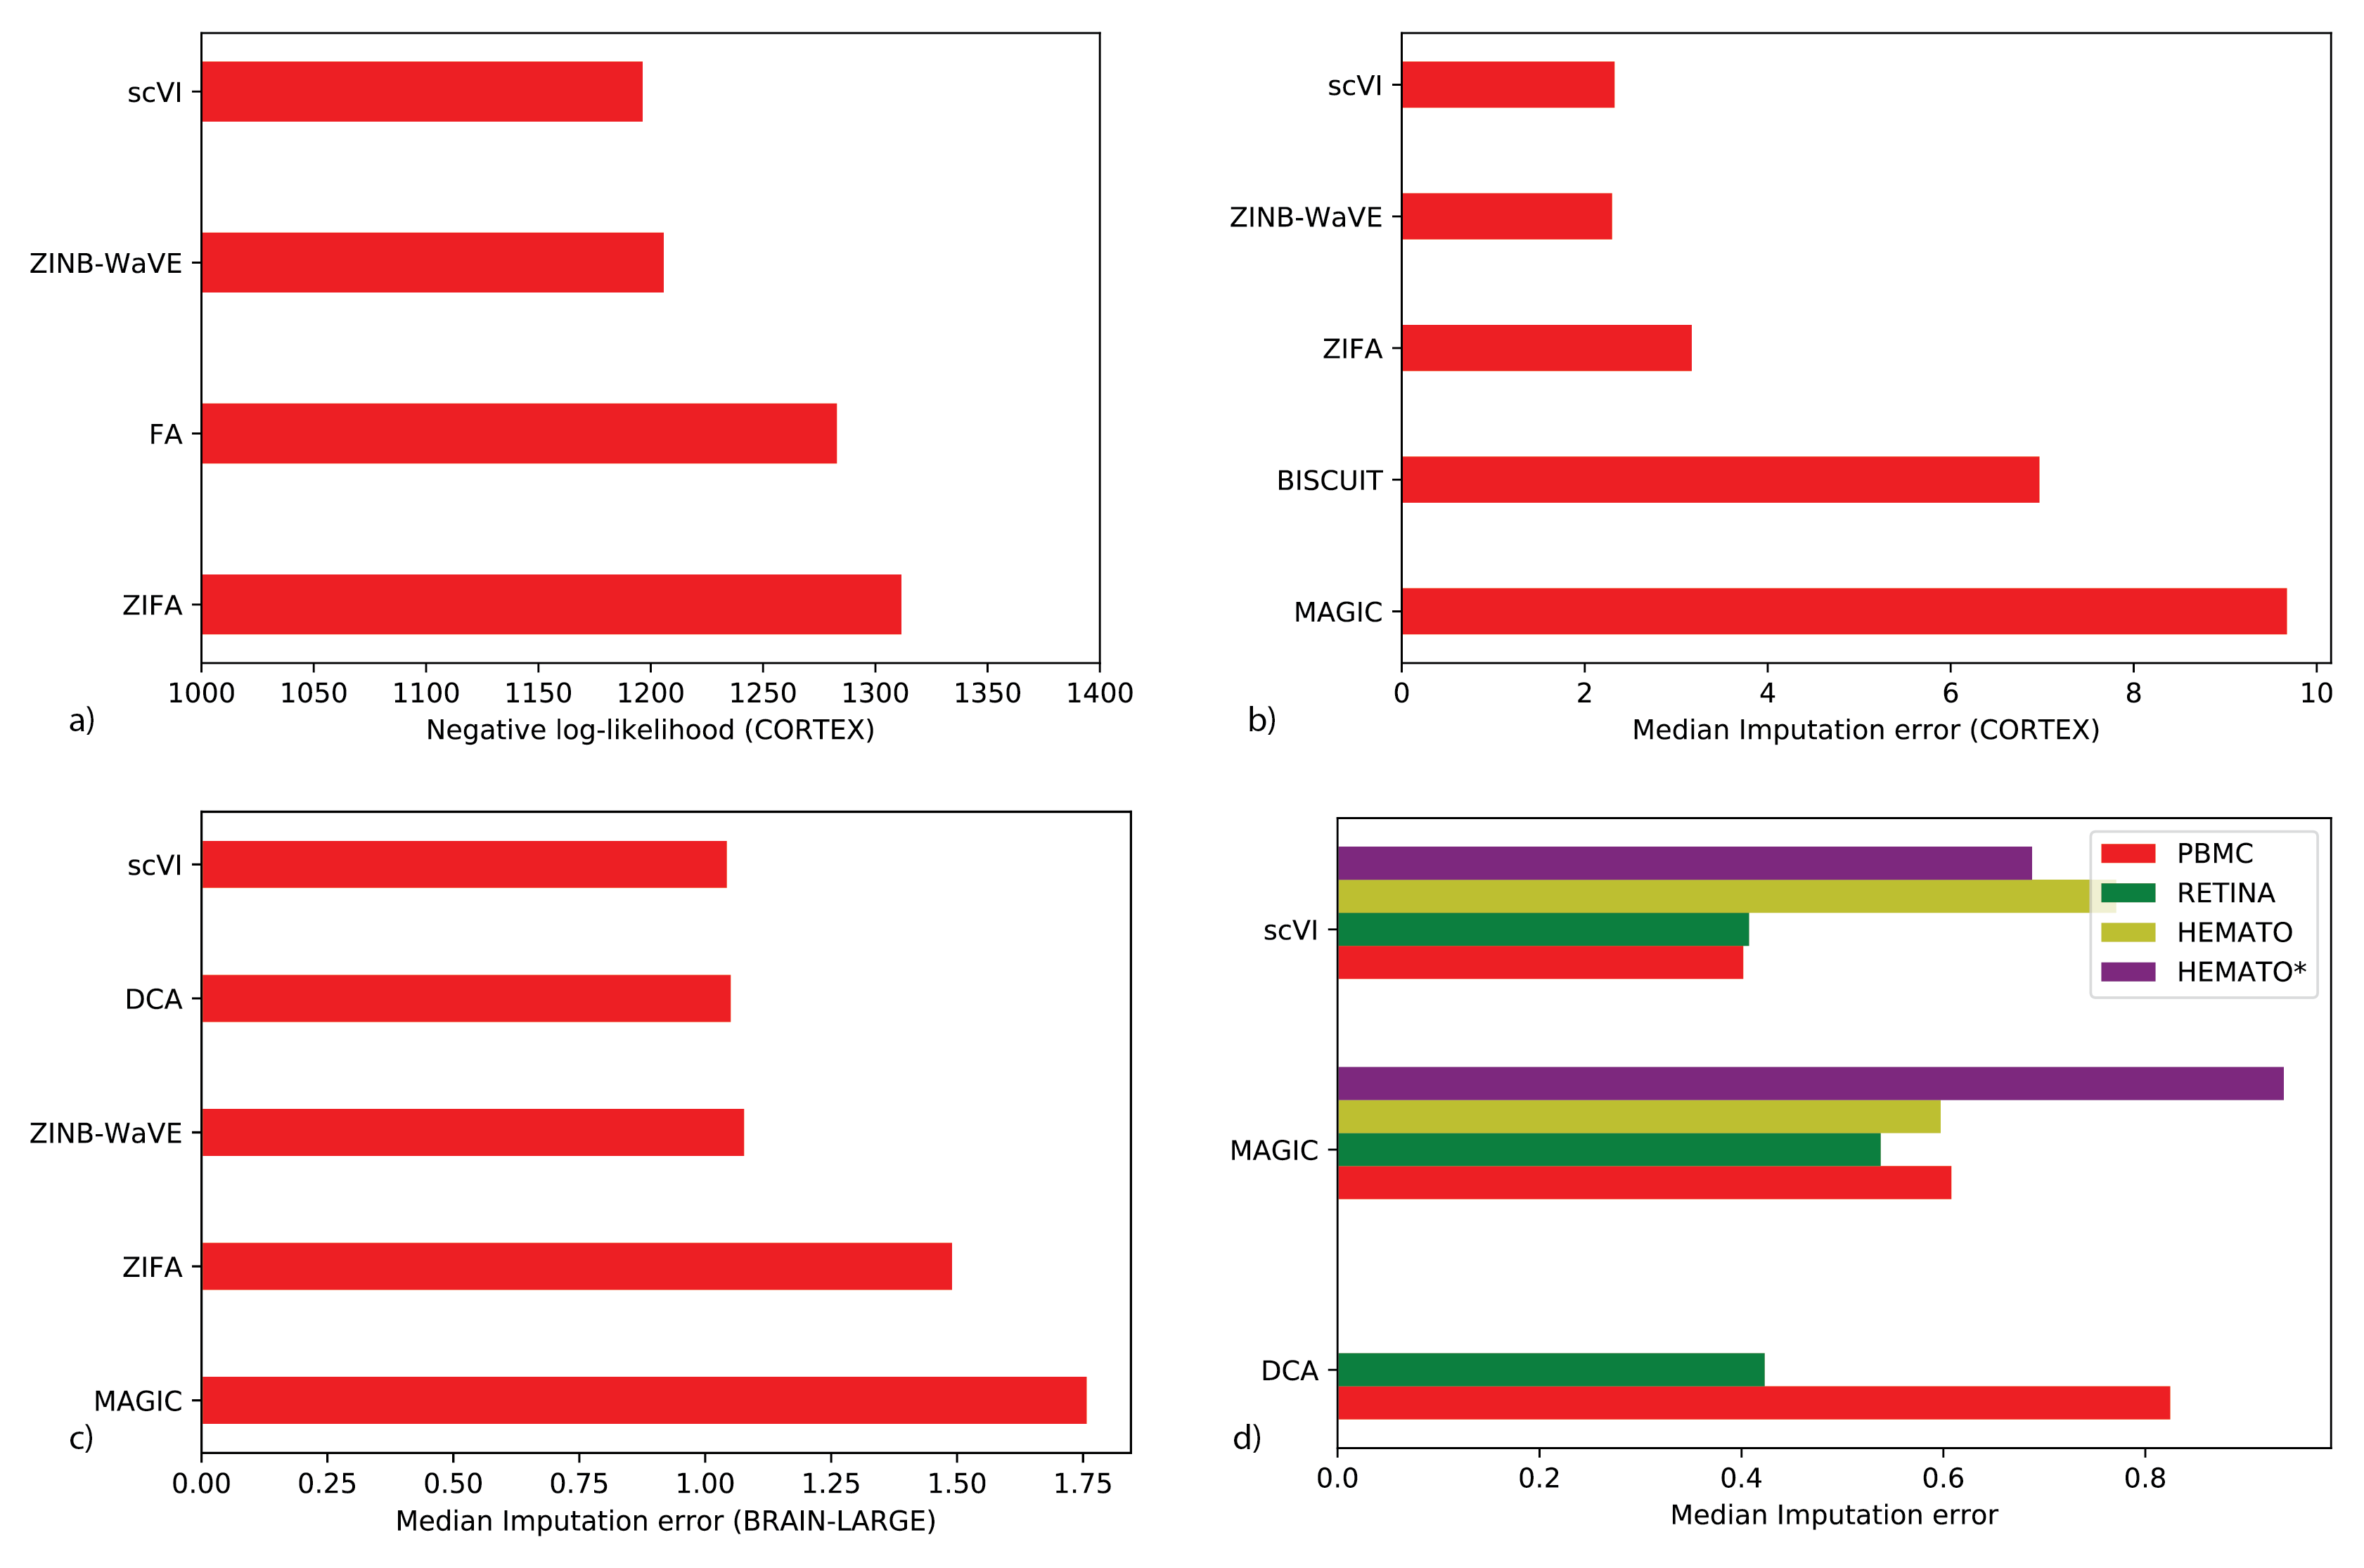
\includegraphics[width=\textwidth]{figures/loglik_imputation_supplement.png}
\caption[Log-likelihood and imputation results]{(a) Log-likelihood results on the CORTEX dataset. (b) through (d): We investigate how scVI latent space can be used to impute the data (with the uniform perturbation scheme) and report benchmarking across datasets for state-of-the-art methods.}
\label{scvilog_imputation_supp}
\end{suppfigure}


\begin{suppfigure}[p]
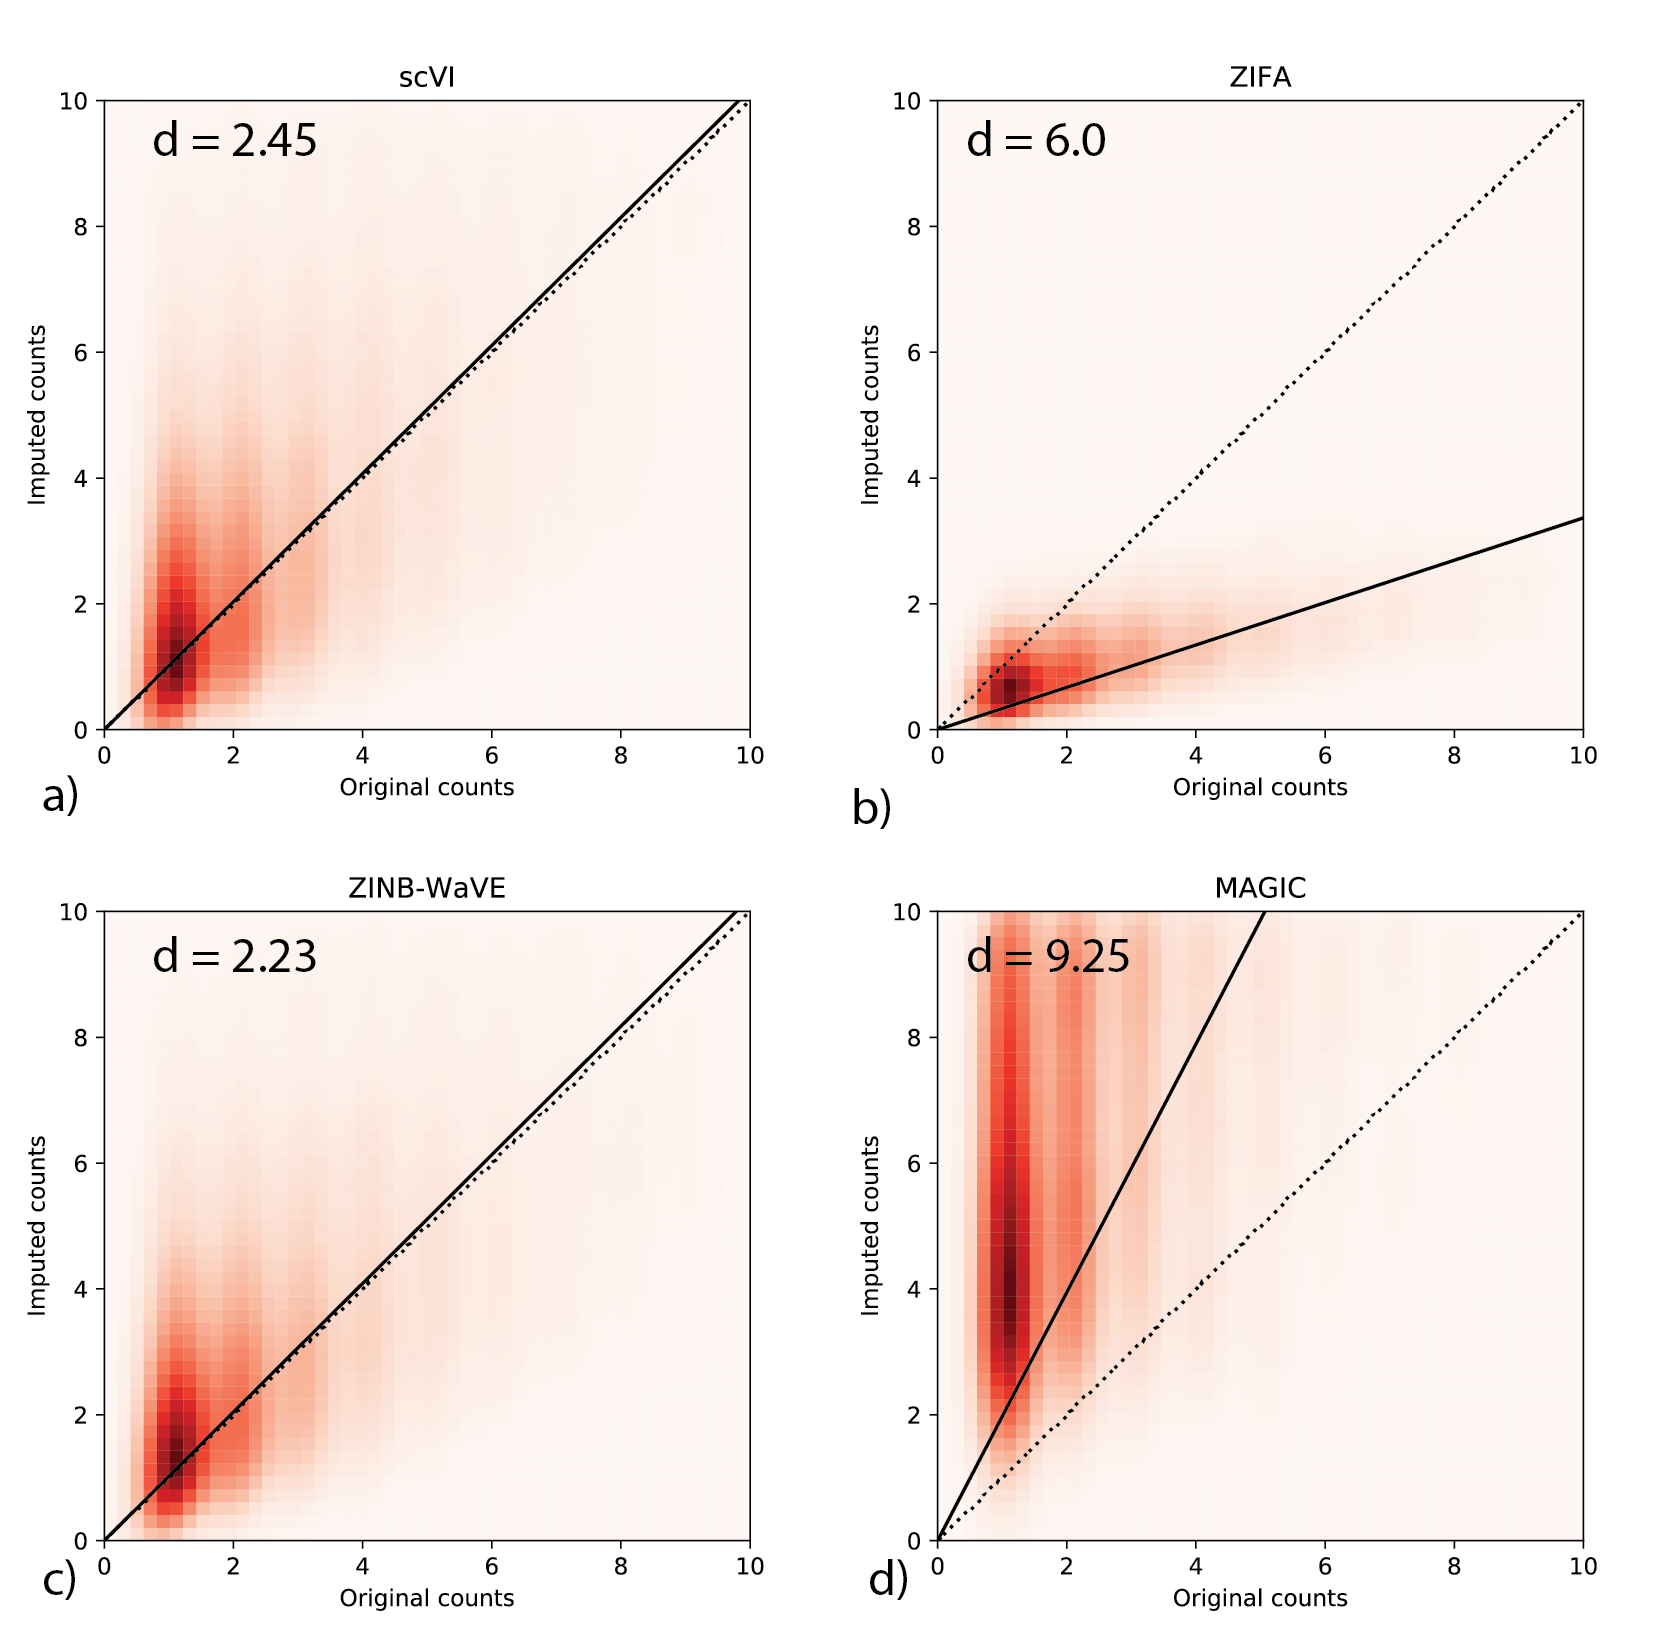
\includegraphics[width=\textwidth]{figures/Figure-3_non_unif.png}
\caption[Non-uniform imputation of scVI on the CORTEX dataset]{Imputation of scVI on the CORTEX dataset. Models are trained on a binomial-down-sampling corrupted dataset (see Methods).  The heatmaps denote density plots of imputed values scVI, ZIFA, MAGIC and ZINB-WaVE on a down-sampled version vs. original values prior to down-sampling. The reported score $d$ is the median imputation error across all the hidden entries (lower is better; see Methods).}
\label{scvilog_imputation_non_unif}
\end{suppfigure}

\begin{suppfigure}[p]
\centering
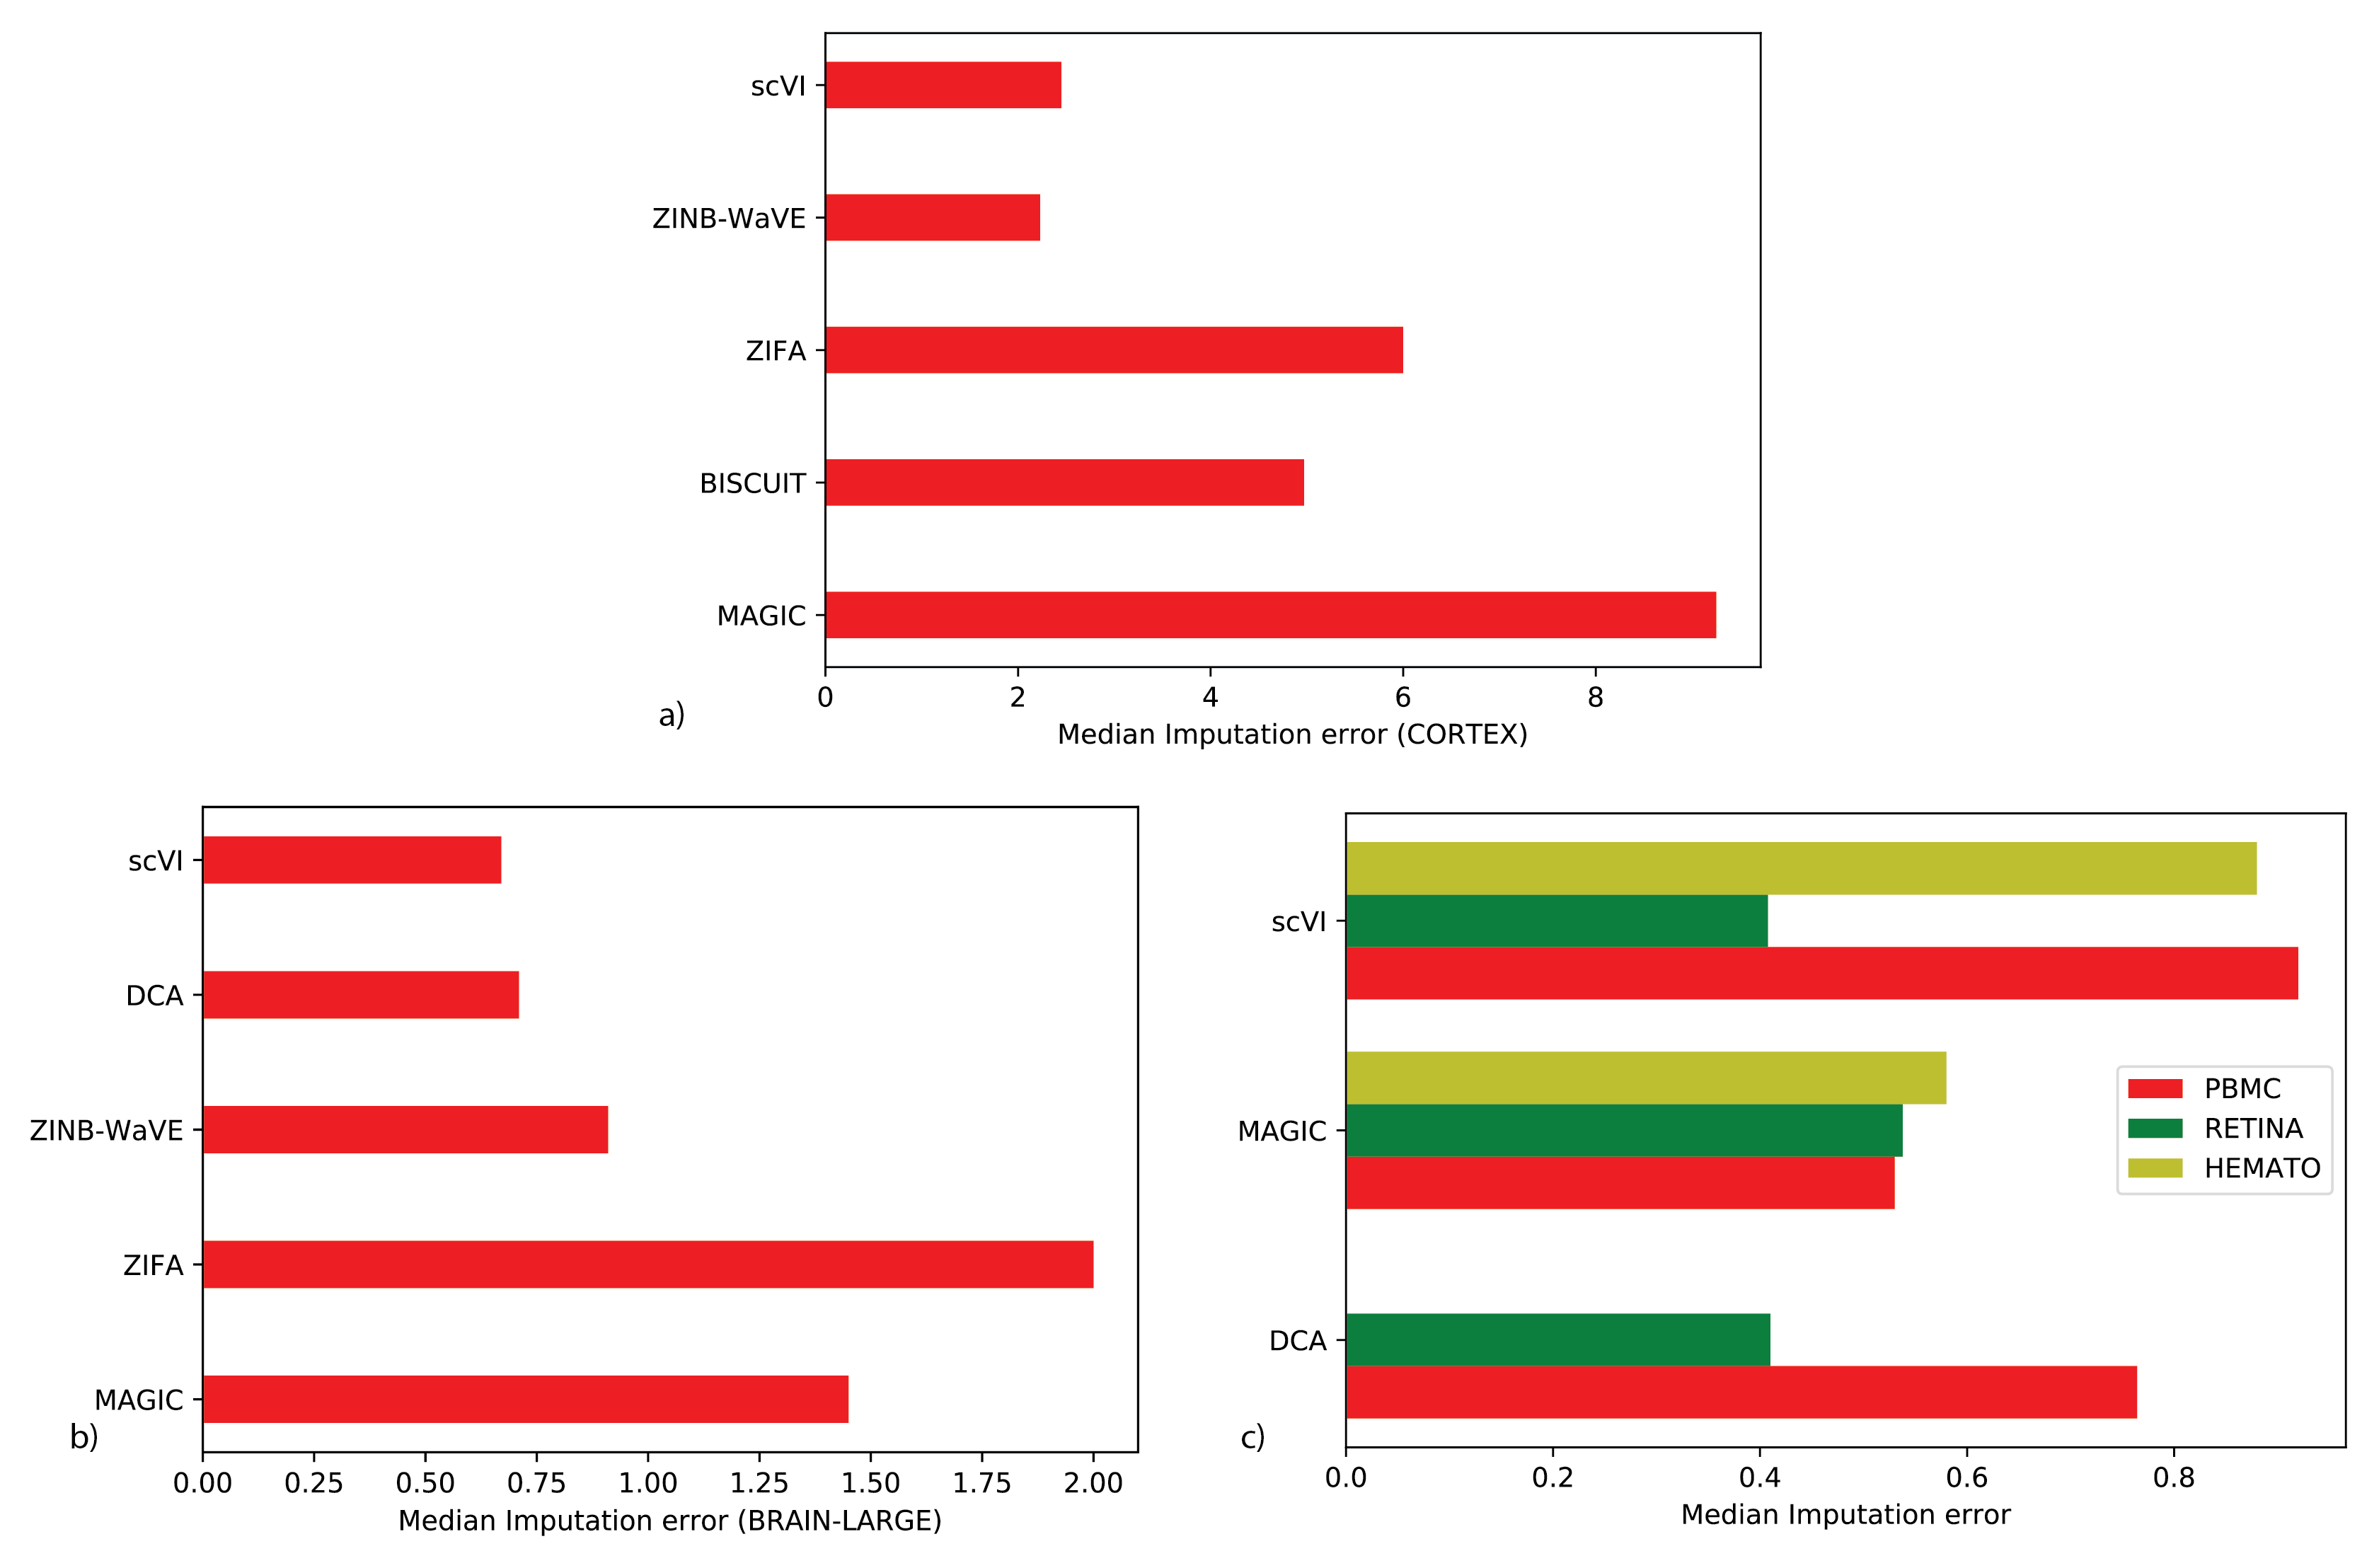
\includegraphics[width=\textwidth]{figures/loglik_imputation_supplement_non_unif.png}
\caption[Non-uniform imputation benchmarking]{(a) through (c): We investigate how scVI latent space can be used to impute the data (with the binomial perturbation scheme) and report benchmarking across datasets for state-of-the-art methods.}
\label{scvilog_imputation_non_unif_supp}
\end{suppfigure}

\begin{suppfigure}[p]
\centering
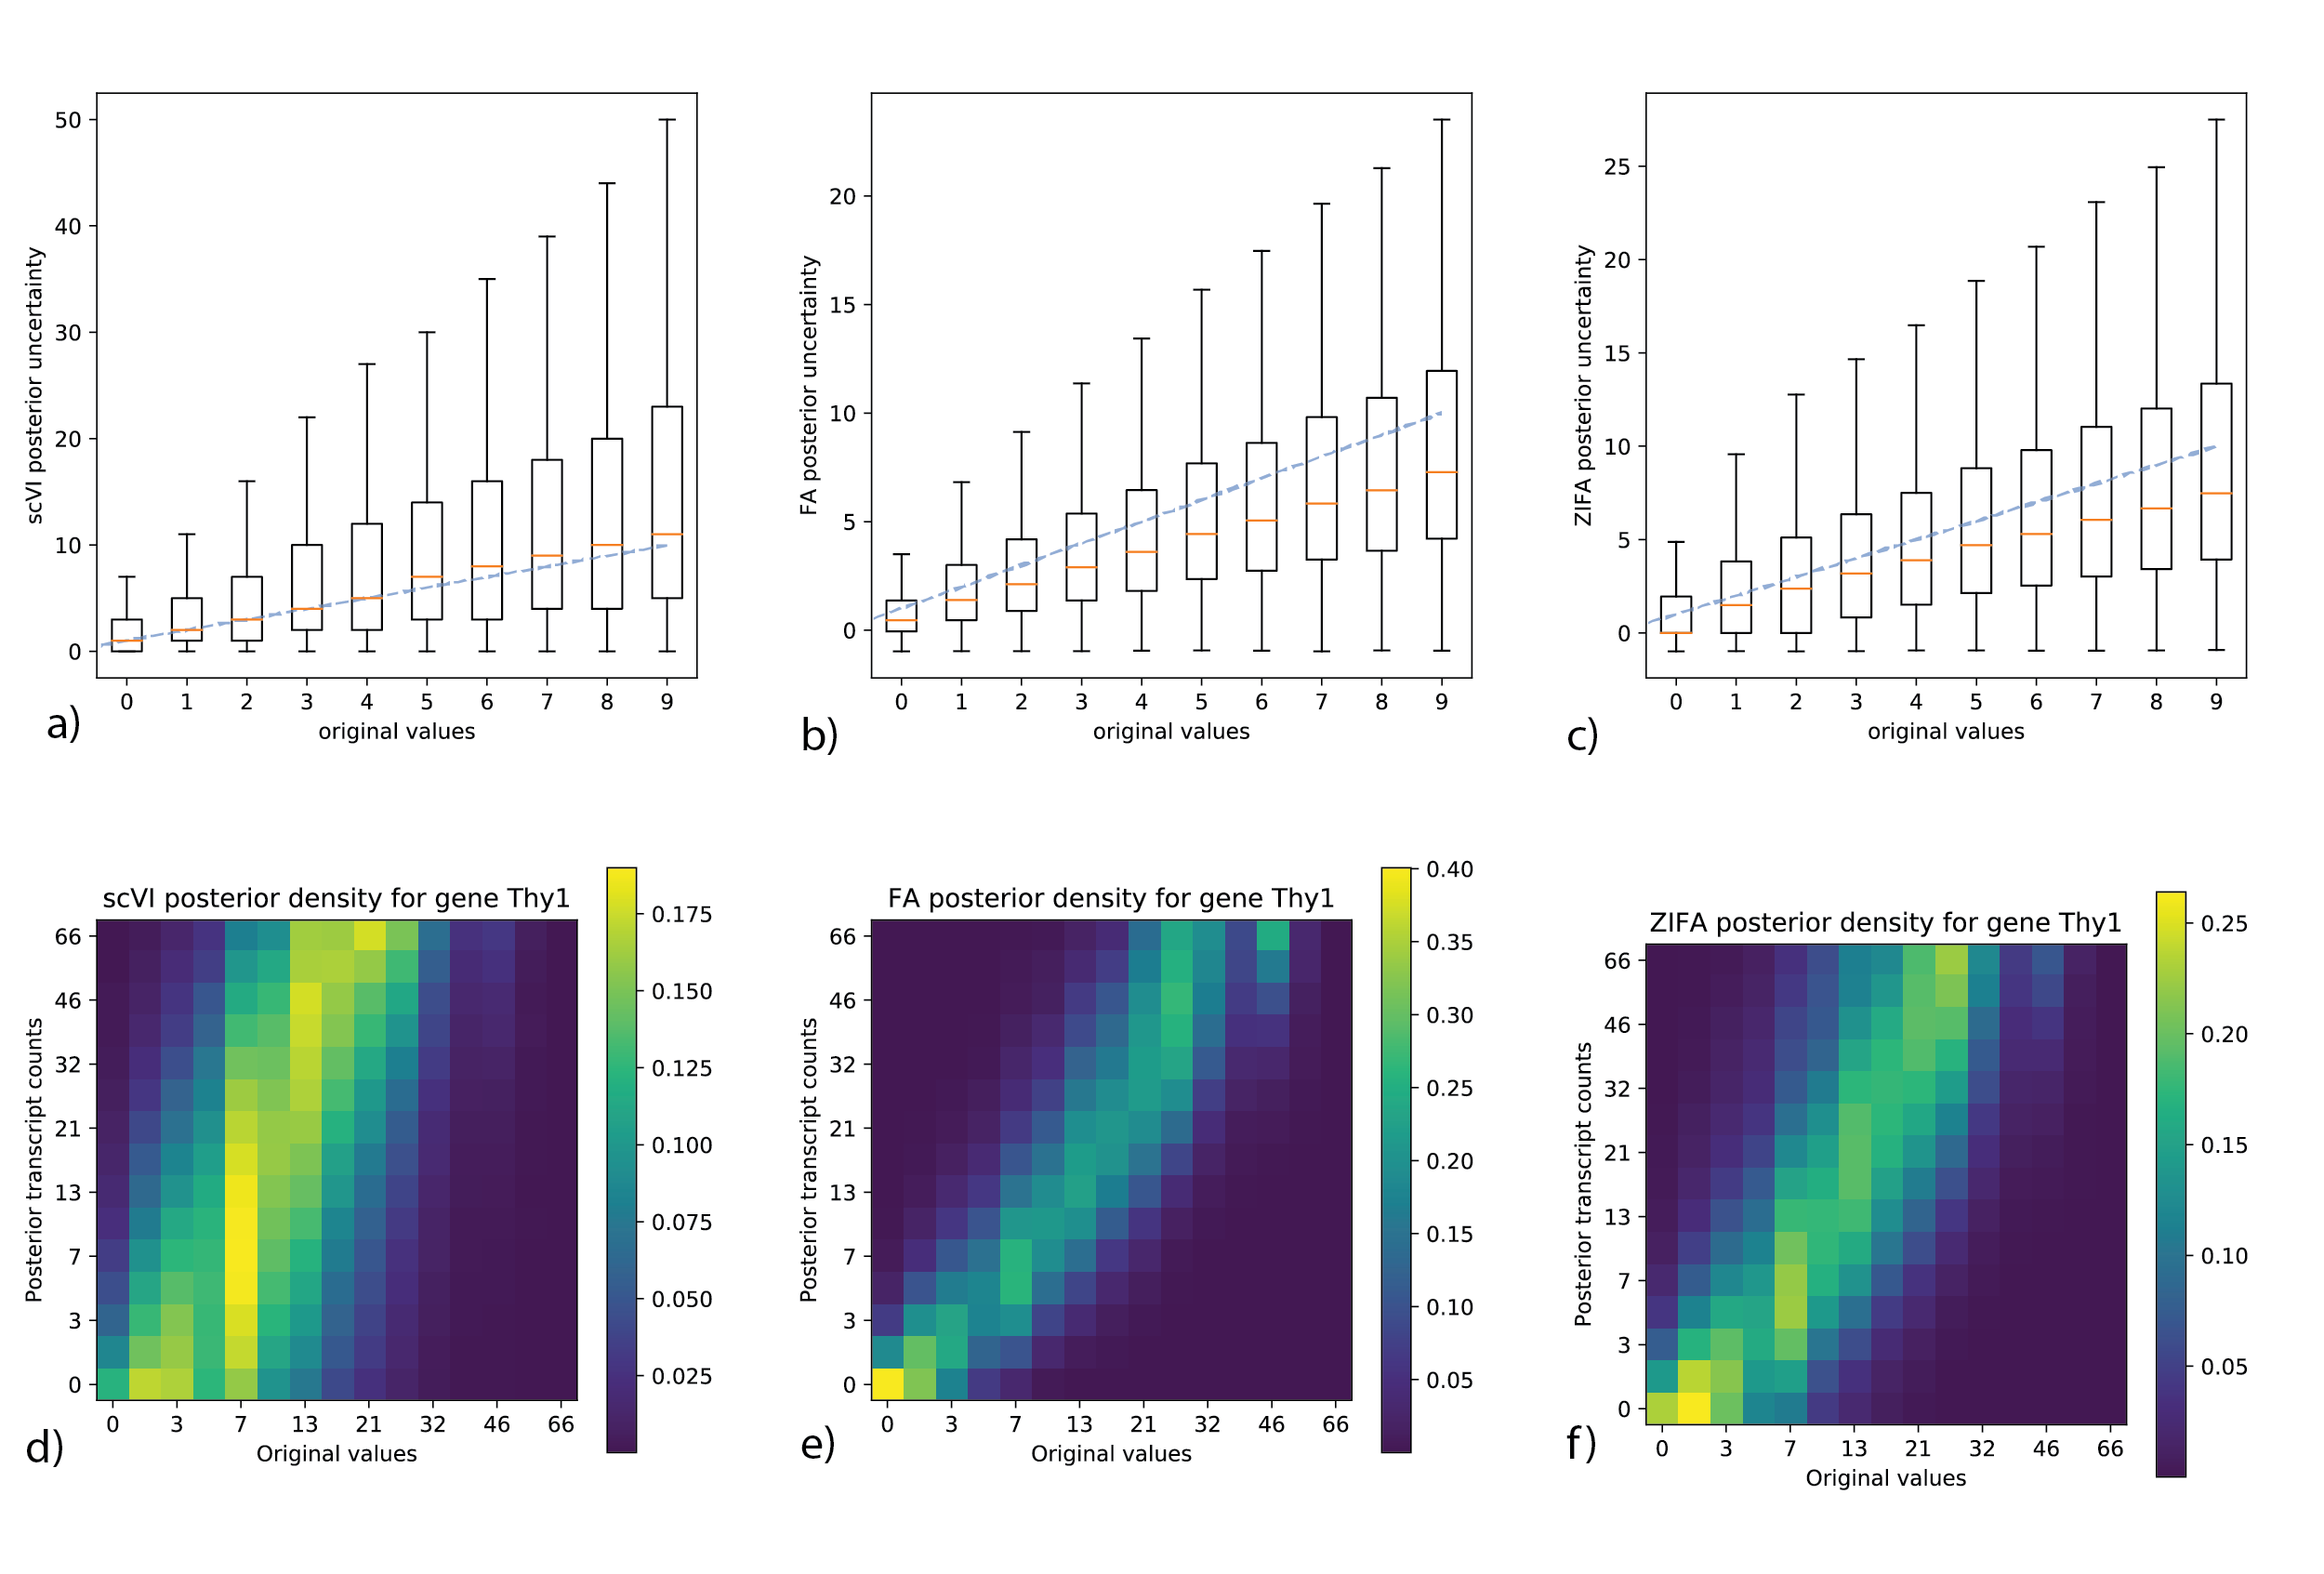
\includegraphics[width=\textwidth]{figures/posterior_supplement.png}
\caption[Posterior analysis of generative models on the CORTEX dataset]{Posterior analysis of generative models on the CORTEX dataset. Panels (a-c) depict the observed counts of randomly selected entries of the data matrix (x-axis) and their posterior uncertainty (y-axis) by sampling from the variational posterior (scVI) or the exact posterior (FA, ZIFA). Whiskers denote the 5th and 95th percentiles. Panels (d-f) represent the observed counts of a representative gene, Thy1, in the CORTEX dataset. Data is presented across all cells ($n=3005$) (x-axis) against the posterior expected counts produced by scVI, ZIFA and FA, respectively (y-axis). The values on each axis have been divided into 20 bins and the color scale reflects the proportion of cells in each pair of bins. By definition, the uncertainty of FA is independent of the input value and tight around the observed count. ZIFA can generate zero and puts realistically more weight in this area. scVI's posterior is more complex, and is able to generate zero for low UMI values but also able to generate high UMI values when the original count observed was only of intermediate intensity.}
\label{scviposterior_supp}
\end{suppfigure}

\begin{suppfigure}
\centering
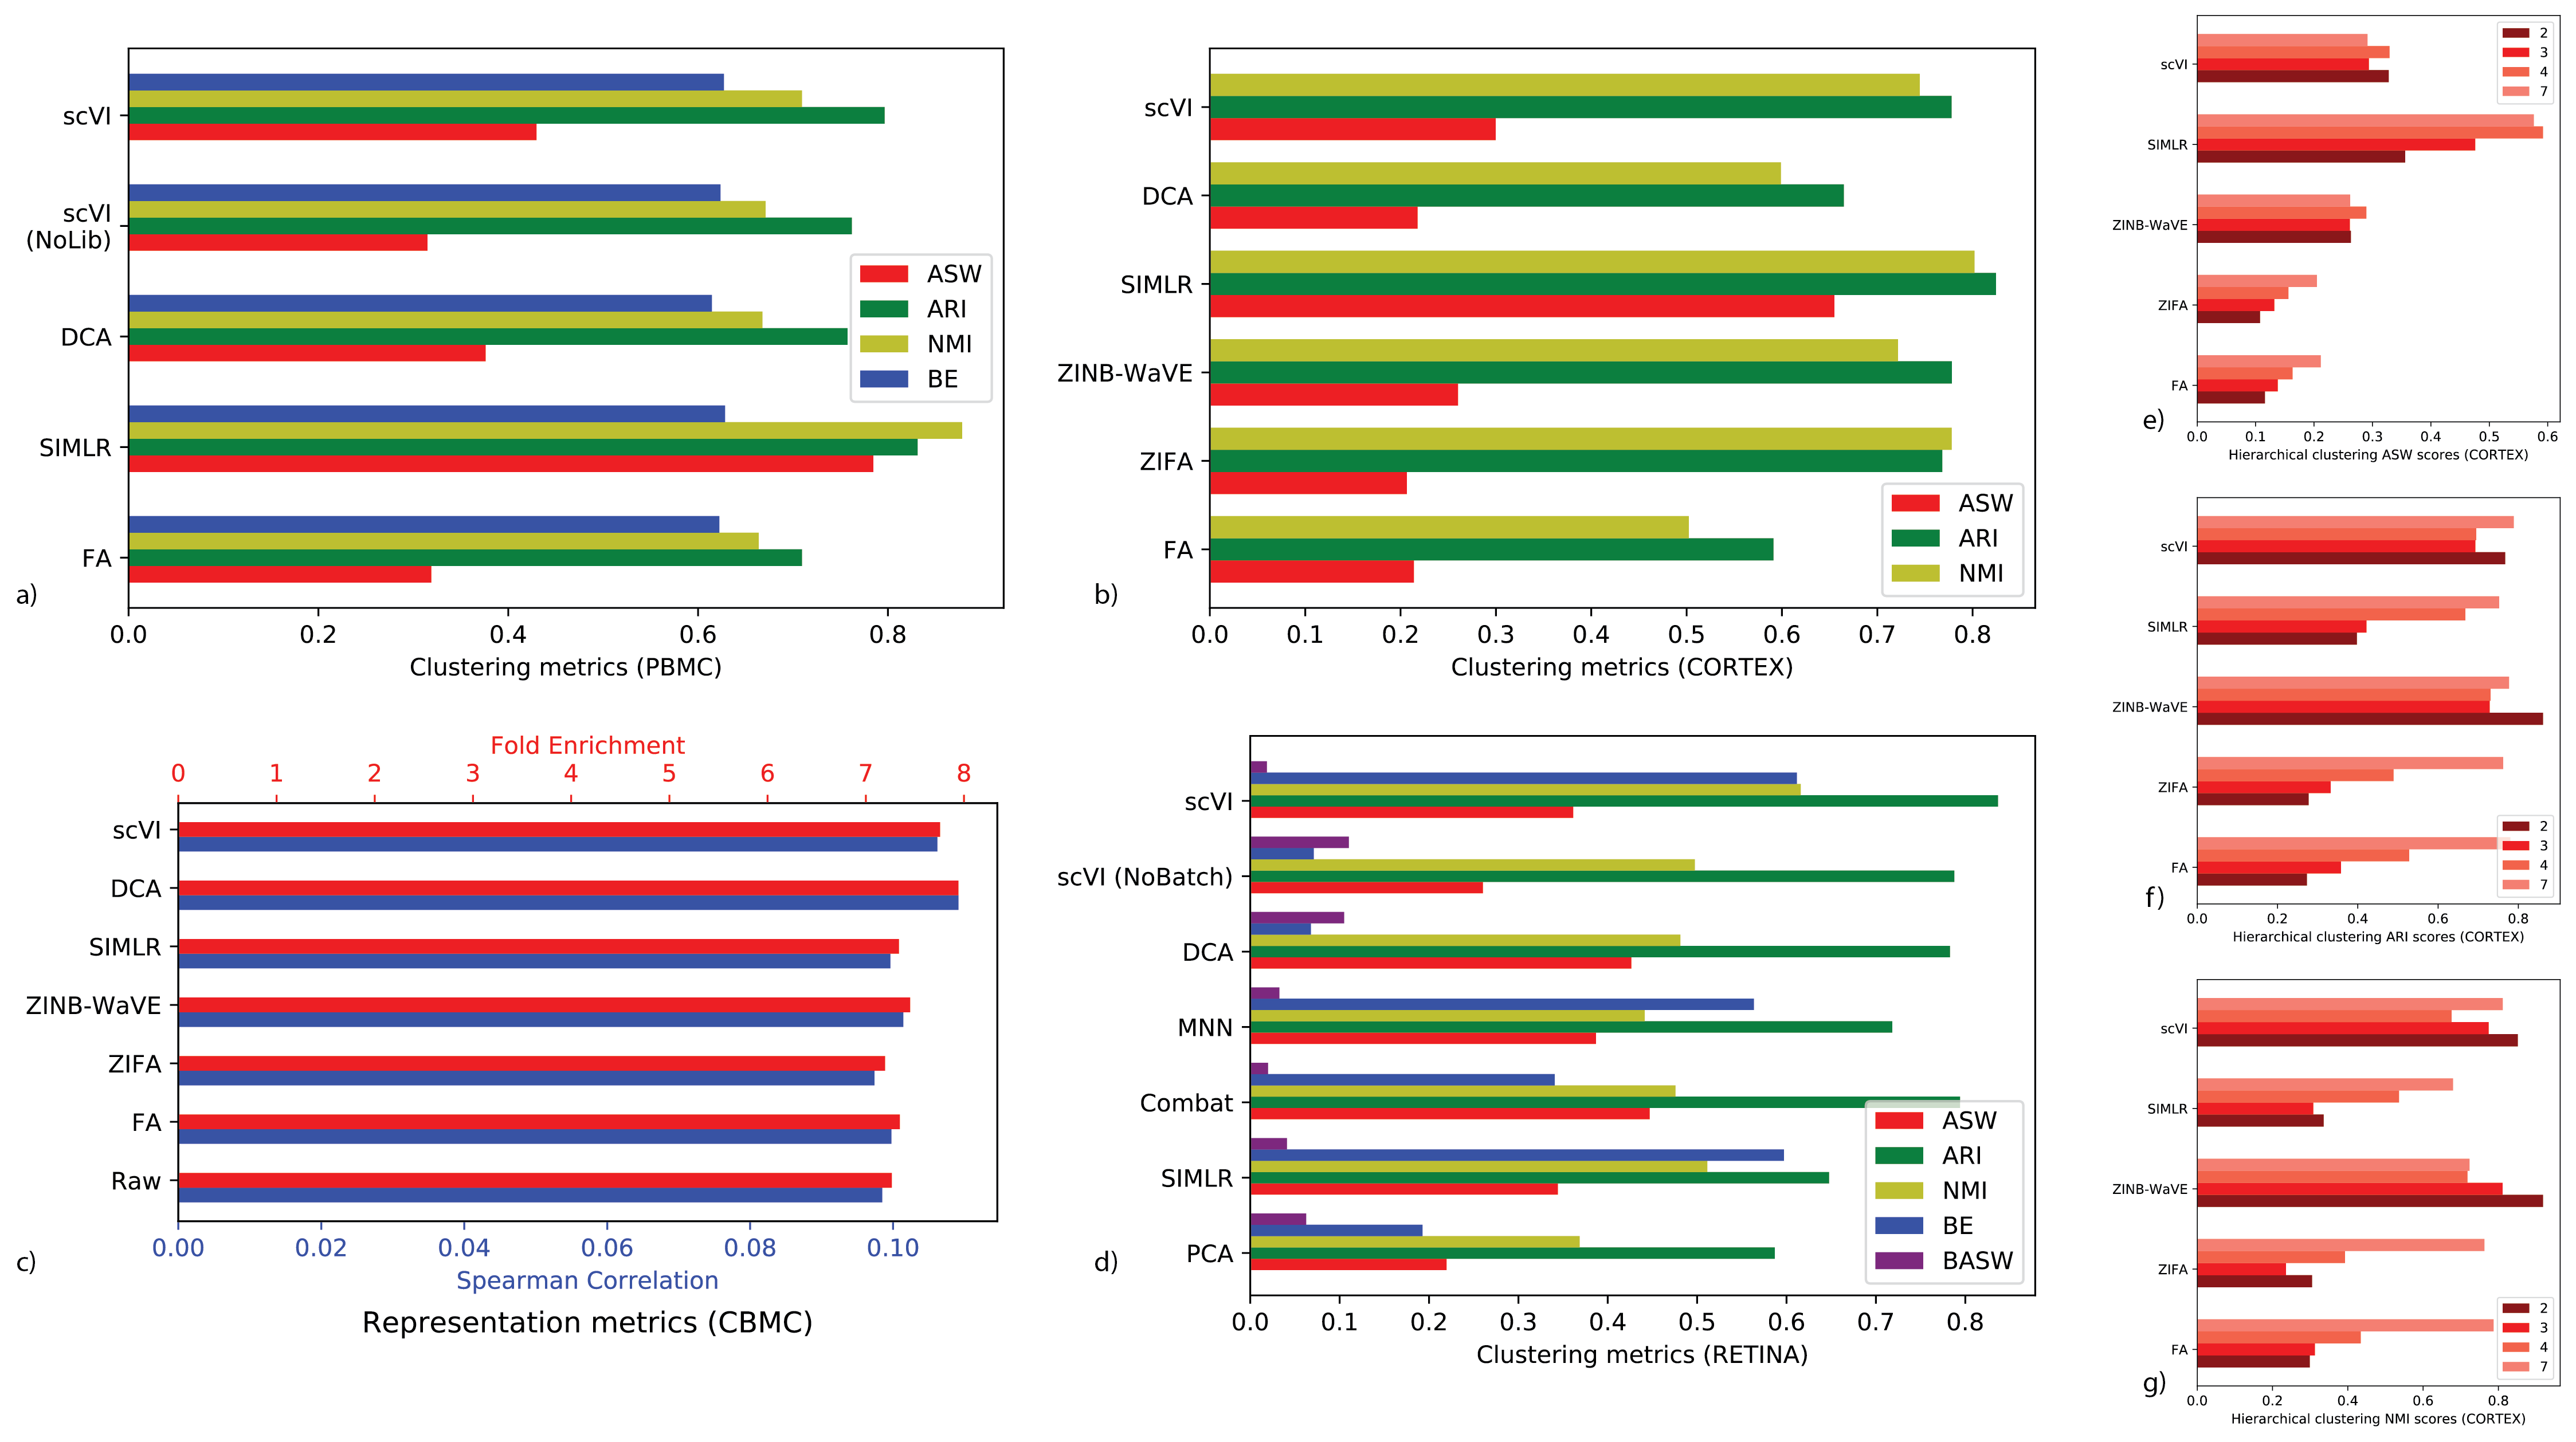
\includegraphics[width=\textwidth]{figures/clustering_supplement.png}
\caption[Clustering performance]{We investigate how scVI latent space can be used to cluster the data and report benchmarking across datasets for state-of-the-art methods. The first four panels depict the results for the (a) PBMC dataset (b) CORTEX (c) CBMC and (d) RETINA. ASW: average silhouette width of pre-annotated subpopulations (higher is better), ARI: adjusted Rand index (higher is better), NMI: normalized mutual information (higher is better), BE: batch-mixing entropy (higher is better), BASW: average silhouette width of batches (lower is better). Panels (e-g) depict the performance of clustering metrics for different depths of the hierarchical clustering in the CORTEX data, computed in the original publication~\cite{Zeisel1138}. The numbers in the legend indicate the number of clusters at the given depth.}
\label{scviclustering_supp}
\end{suppfigure}

\begin{suppfigure}
\centering
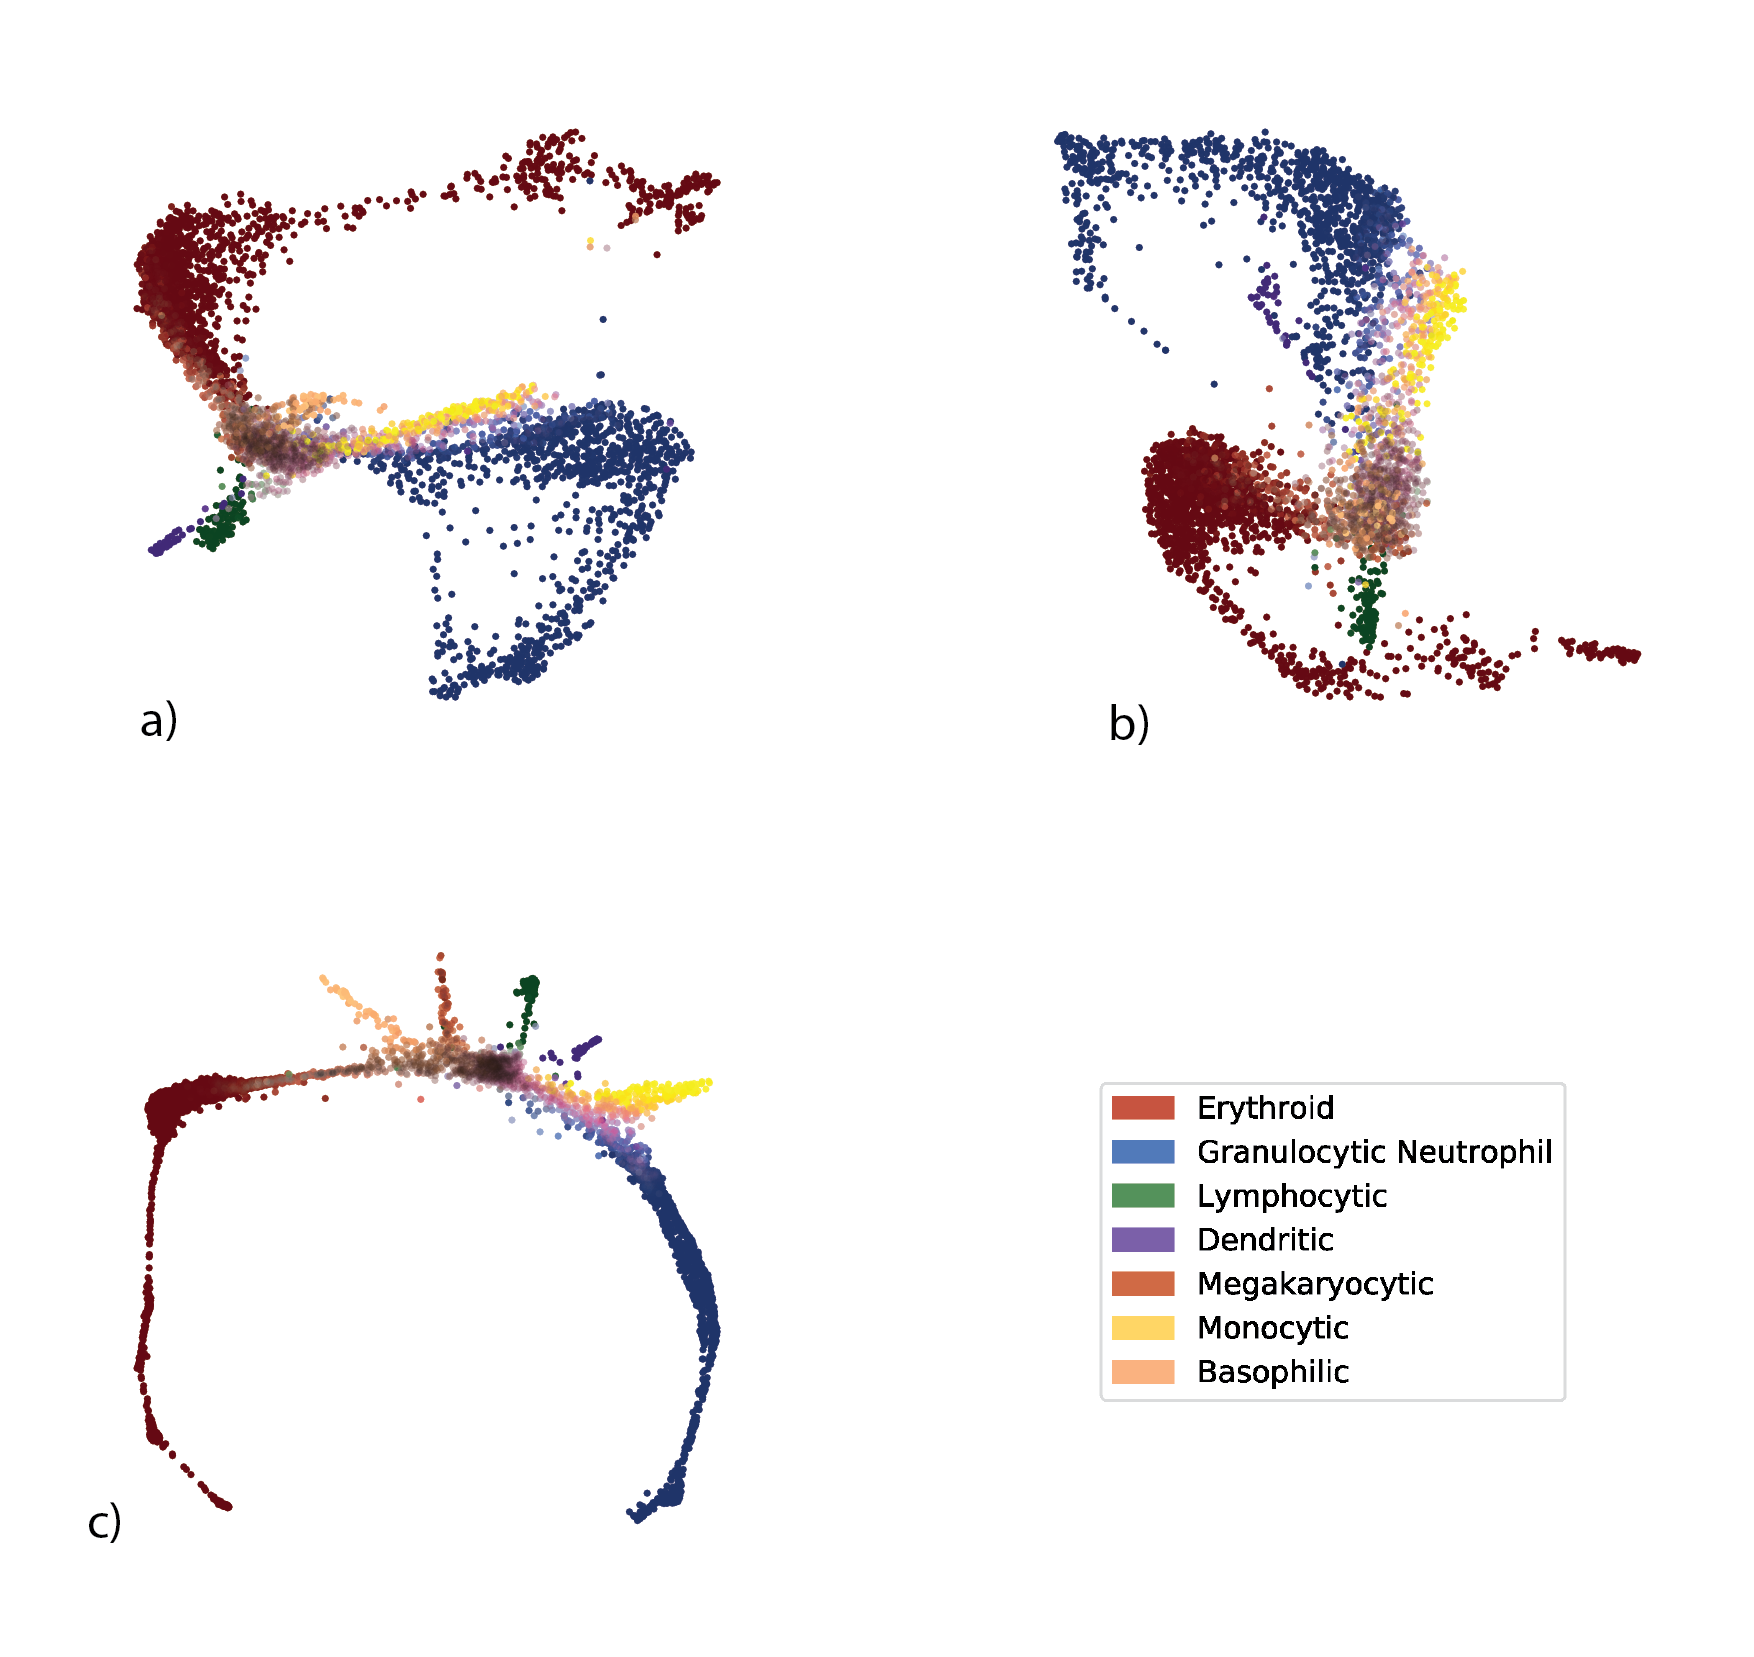
\includegraphics[width=\textwidth]{figures/hemato_supp.png}
\caption[Additional comparison of scVI and PCA on the HEMATO dataset]{Additional comparison of scVI and PCA on the HEMATO dataset. All scatter plots illustrate the embedding of a 5-nearest neighbors graph of a latent space. Cells positions are computed using a force-directed layout; (a) denotes a reduction to 60 pcs as in the original paper. (b) denotes the output of a scVI in dimension 60. As the dimension is sensibly different from other experiments, the warm-up schedule (which governs how the prior on $z$ is enforced) was adjusted. (c) denotes the figure from the main paper. To recover all the differentiation paths, the authors performed several operations on the $K$-nearest neighbors graph that we did not reproduce in this analysis. We instead visualize the graph before the smoothing procedure.}
\label{scvihemato_supp}
\end{suppfigure}


\begin{suppfigure}
\centering
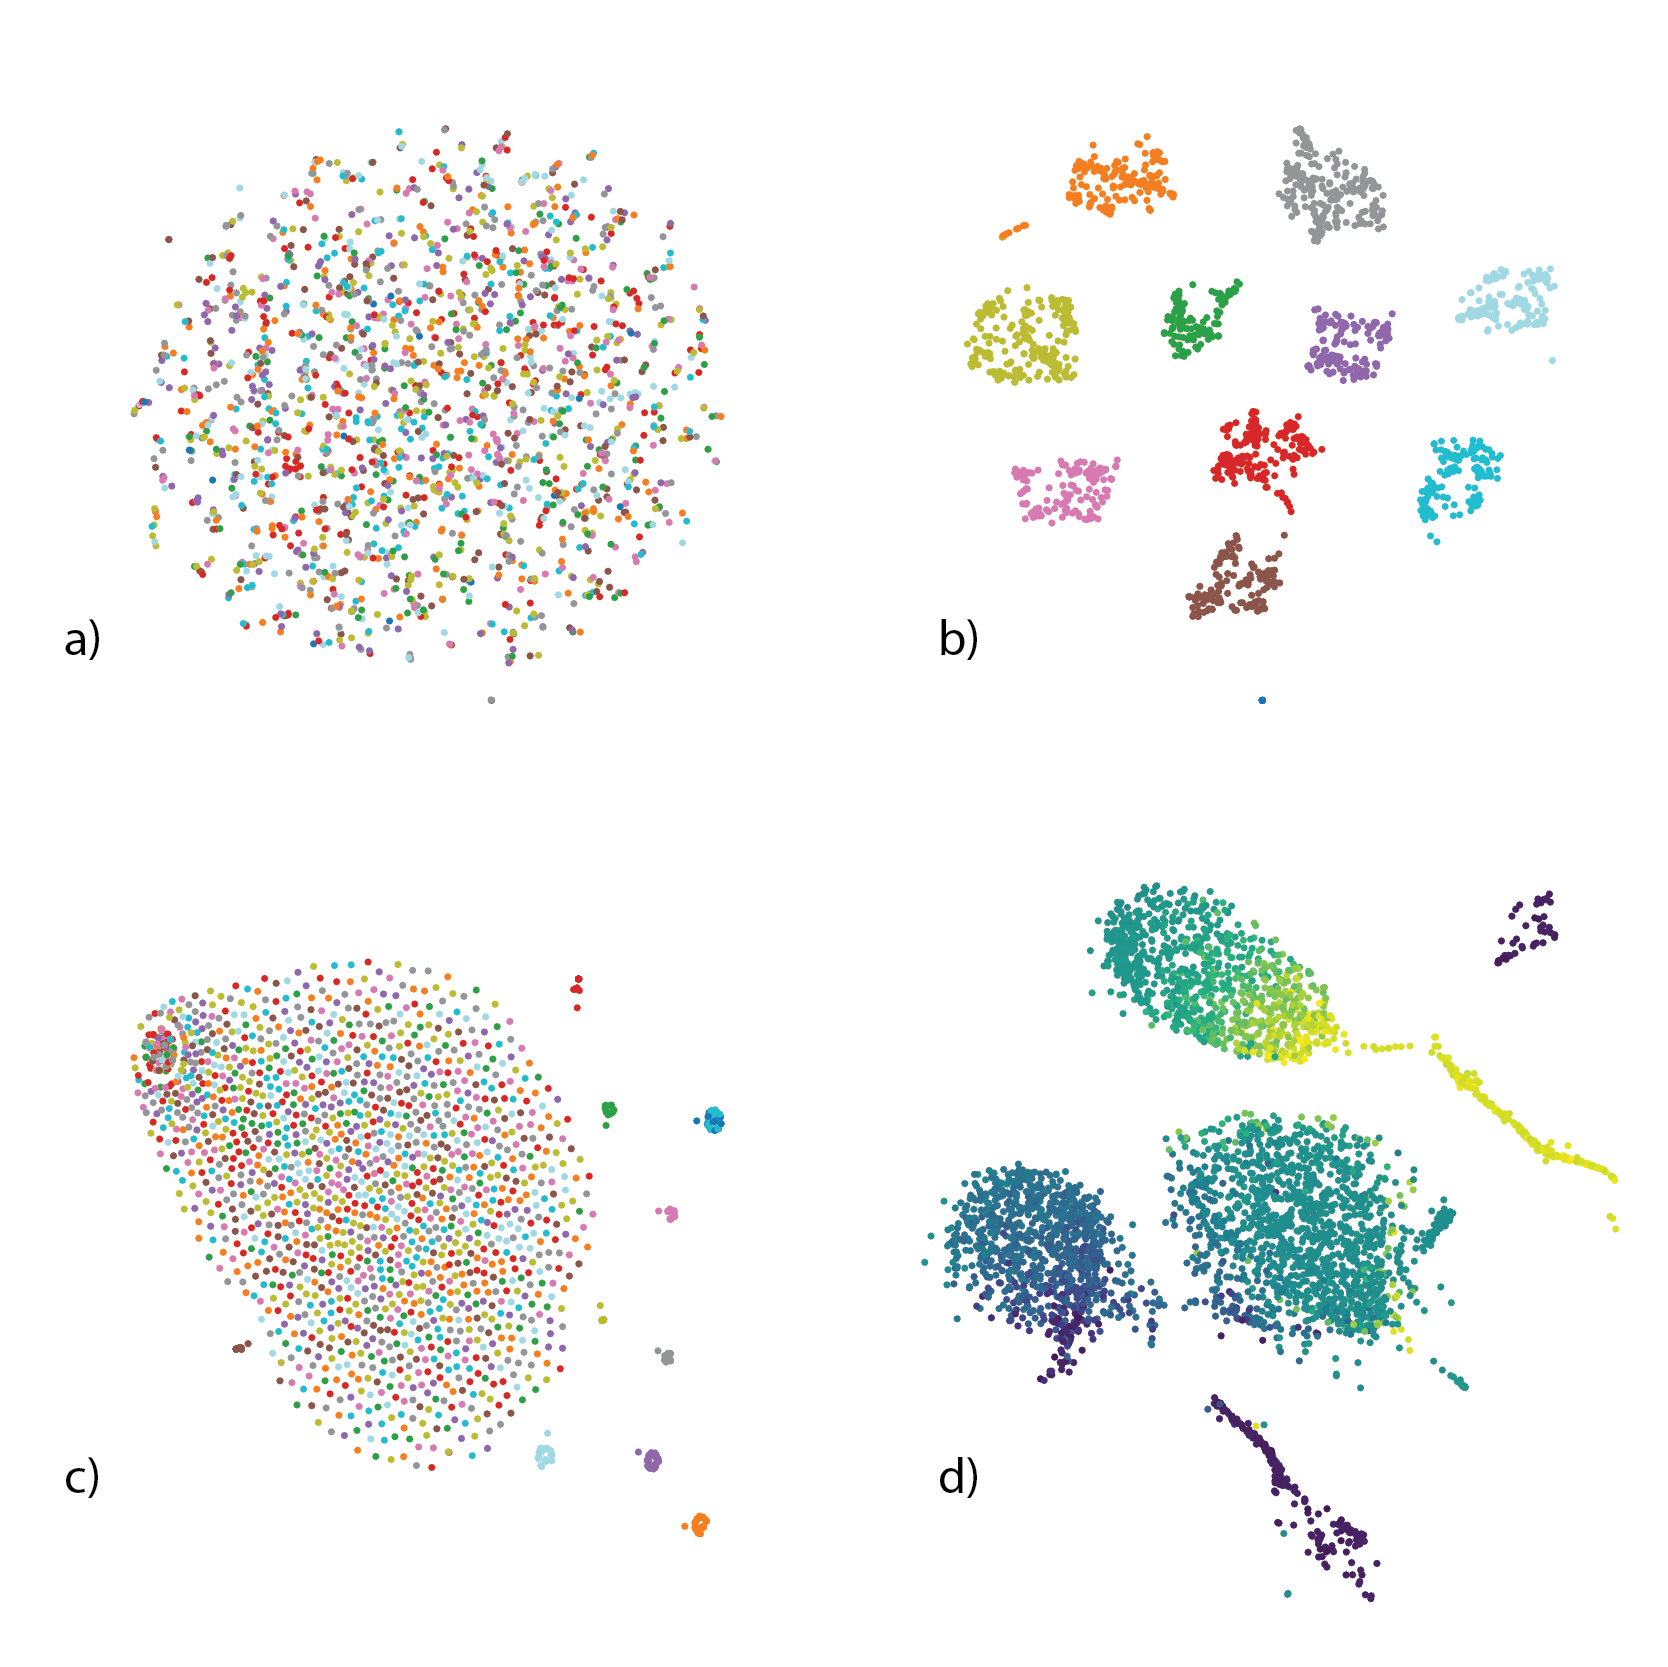
\includegraphics[width=\textwidth]{figures/SIMLR_supplement.png}
\caption[Details for the clustering panel]{Details for the clustering panel. For the random data, we obtain the labels that order the cell-cell similarity matrices by a k-means clustering on SIMLR latent space. (a) scVI latent space with SIMLR labels. There is no structure. (b) SIMLR latent space with SIMLR labels. (c) PCA latent space with SIMLR labels. (d) SIMLR tSNE on the HEMATO dataset. We prefer to visualize the SIMLR embedding on a kNN graph since the continuum structure of the dataset would be lost, even with tSNE.}
\label{scvisuppfig2}
\end{suppfigure}


\begin{suppfigure}[htp]
  \centering
  \begin{subfigure}[b]{0.3\textwidth}
        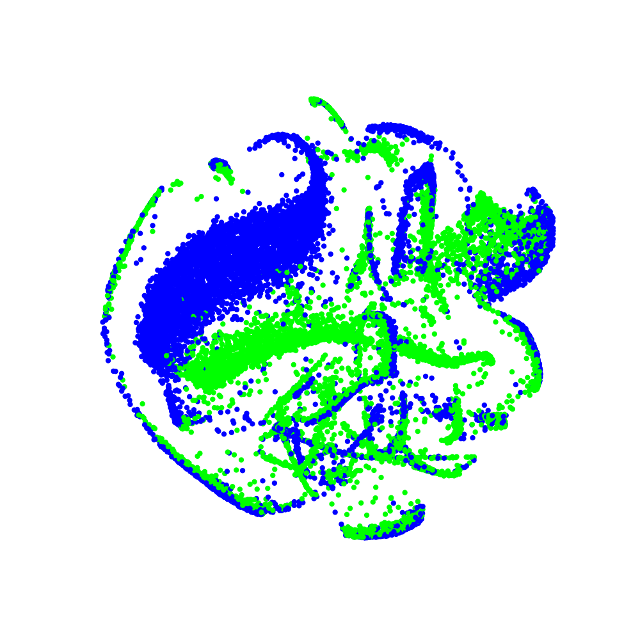
\includegraphics[width=\textwidth]{figures/PCA_tSNE_bipolar_batch.png}
        \caption{tSNE embedding for PCA, colored by batch}
    \end{subfigure}
\hspace{5pt}
  \begin{subfigure}[b]{0.3\textwidth}
        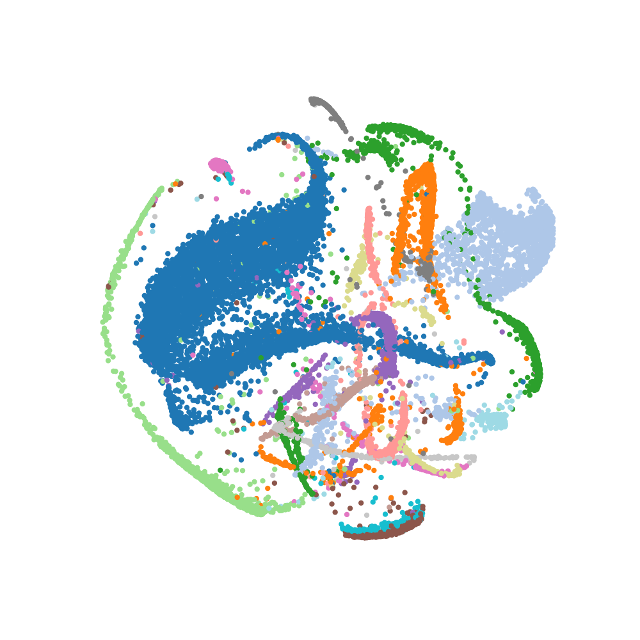
\includegraphics[width=\textwidth]{figures/PCA_tSNE_bipolar_clusters.png}
        \caption{tSNE embedding for PCA, colored by cell type}
    \end{subfigure}
  \hspace{5pt}
    \begin{subfigure}[b]{0.3\textwidth}
        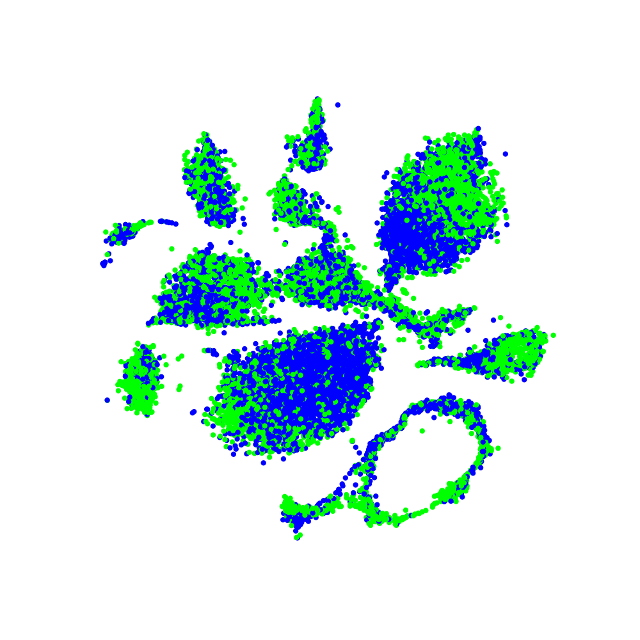
\includegraphics[width=\textwidth]{figures/SIMLR_tSNE_bipolar_batch.png}
        \caption{Embedding for SIMLR, colored by batch}
    \end{subfigure}
  \hspace{5pt}
      \begin{subfigure}[b]{0.3\textwidth}
        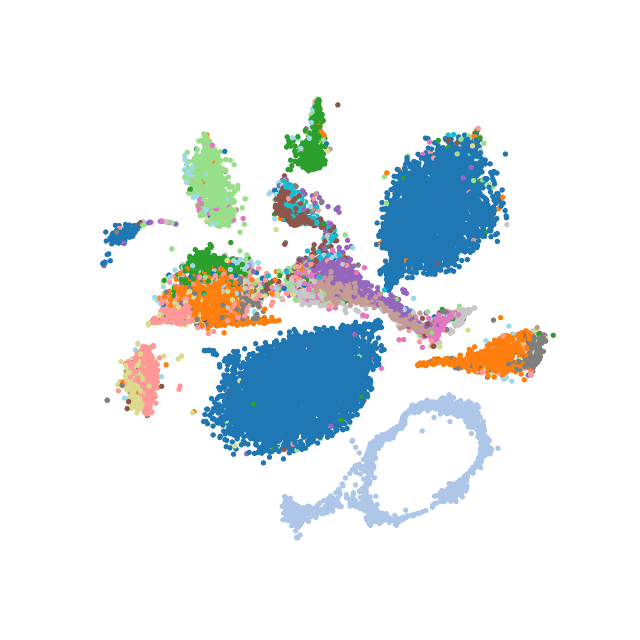
\includegraphics[width=\textwidth]{figures/SIMLR_tSNE_bipolar_clusters.png}
        \caption{Embedding for SIMLR, colored by cell type}
    \end{subfigure}
  \hspace{5pt}
      \begin{subfigure}[b]{0.3\textwidth}
        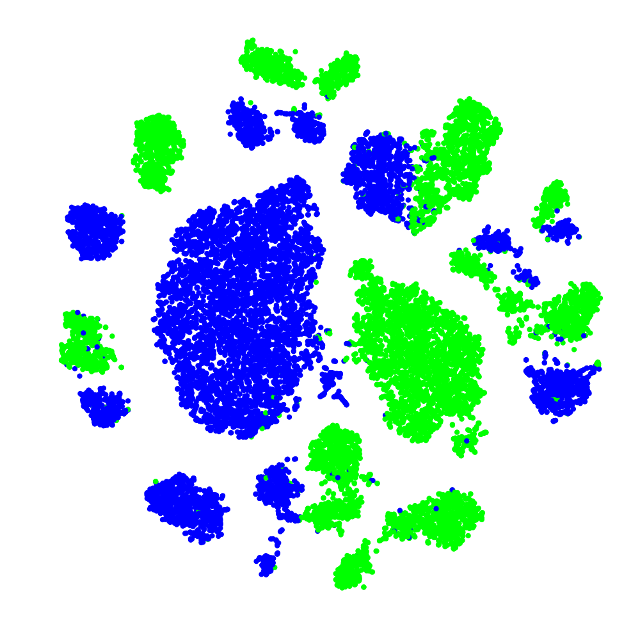
\includegraphics[width=\textwidth]{figures/DCA_tSNE_bipolar_batch.png}
        \caption{Embedding for DCA, colored by batch}
    \end{subfigure}
  \hspace{5pt}
      \begin{subfigure}[b]{0.3\textwidth}
        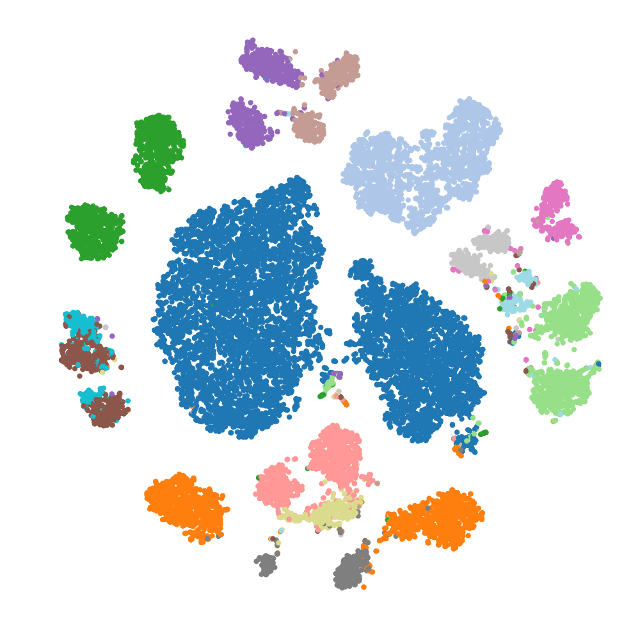
\includegraphics[width=\textwidth]{figures/DCA_tSNE_bipolar_clusters.png}
        \caption{Embedding for DCA, colored by cell type}
    \end{subfigure}
  \caption[Batch effect removal on the RETINA dataset]{Batch effect removal on the RETINA dataset. (a, b) Embedding plots for PCA were generated by applying tSNE on the respective latent space. (c, d) For SIMLR, we used the tSNE coordinates provided by the program and the number of clusters was set to the number of pre-annotated subpopulations ($n=15$). (e, f) Embedding plots for DCA were generated by applying tSNE on the respective latent space.}
  \label{scviMNNfigure}
\end{suppfigure}


\begin{suppfigure}
\centering
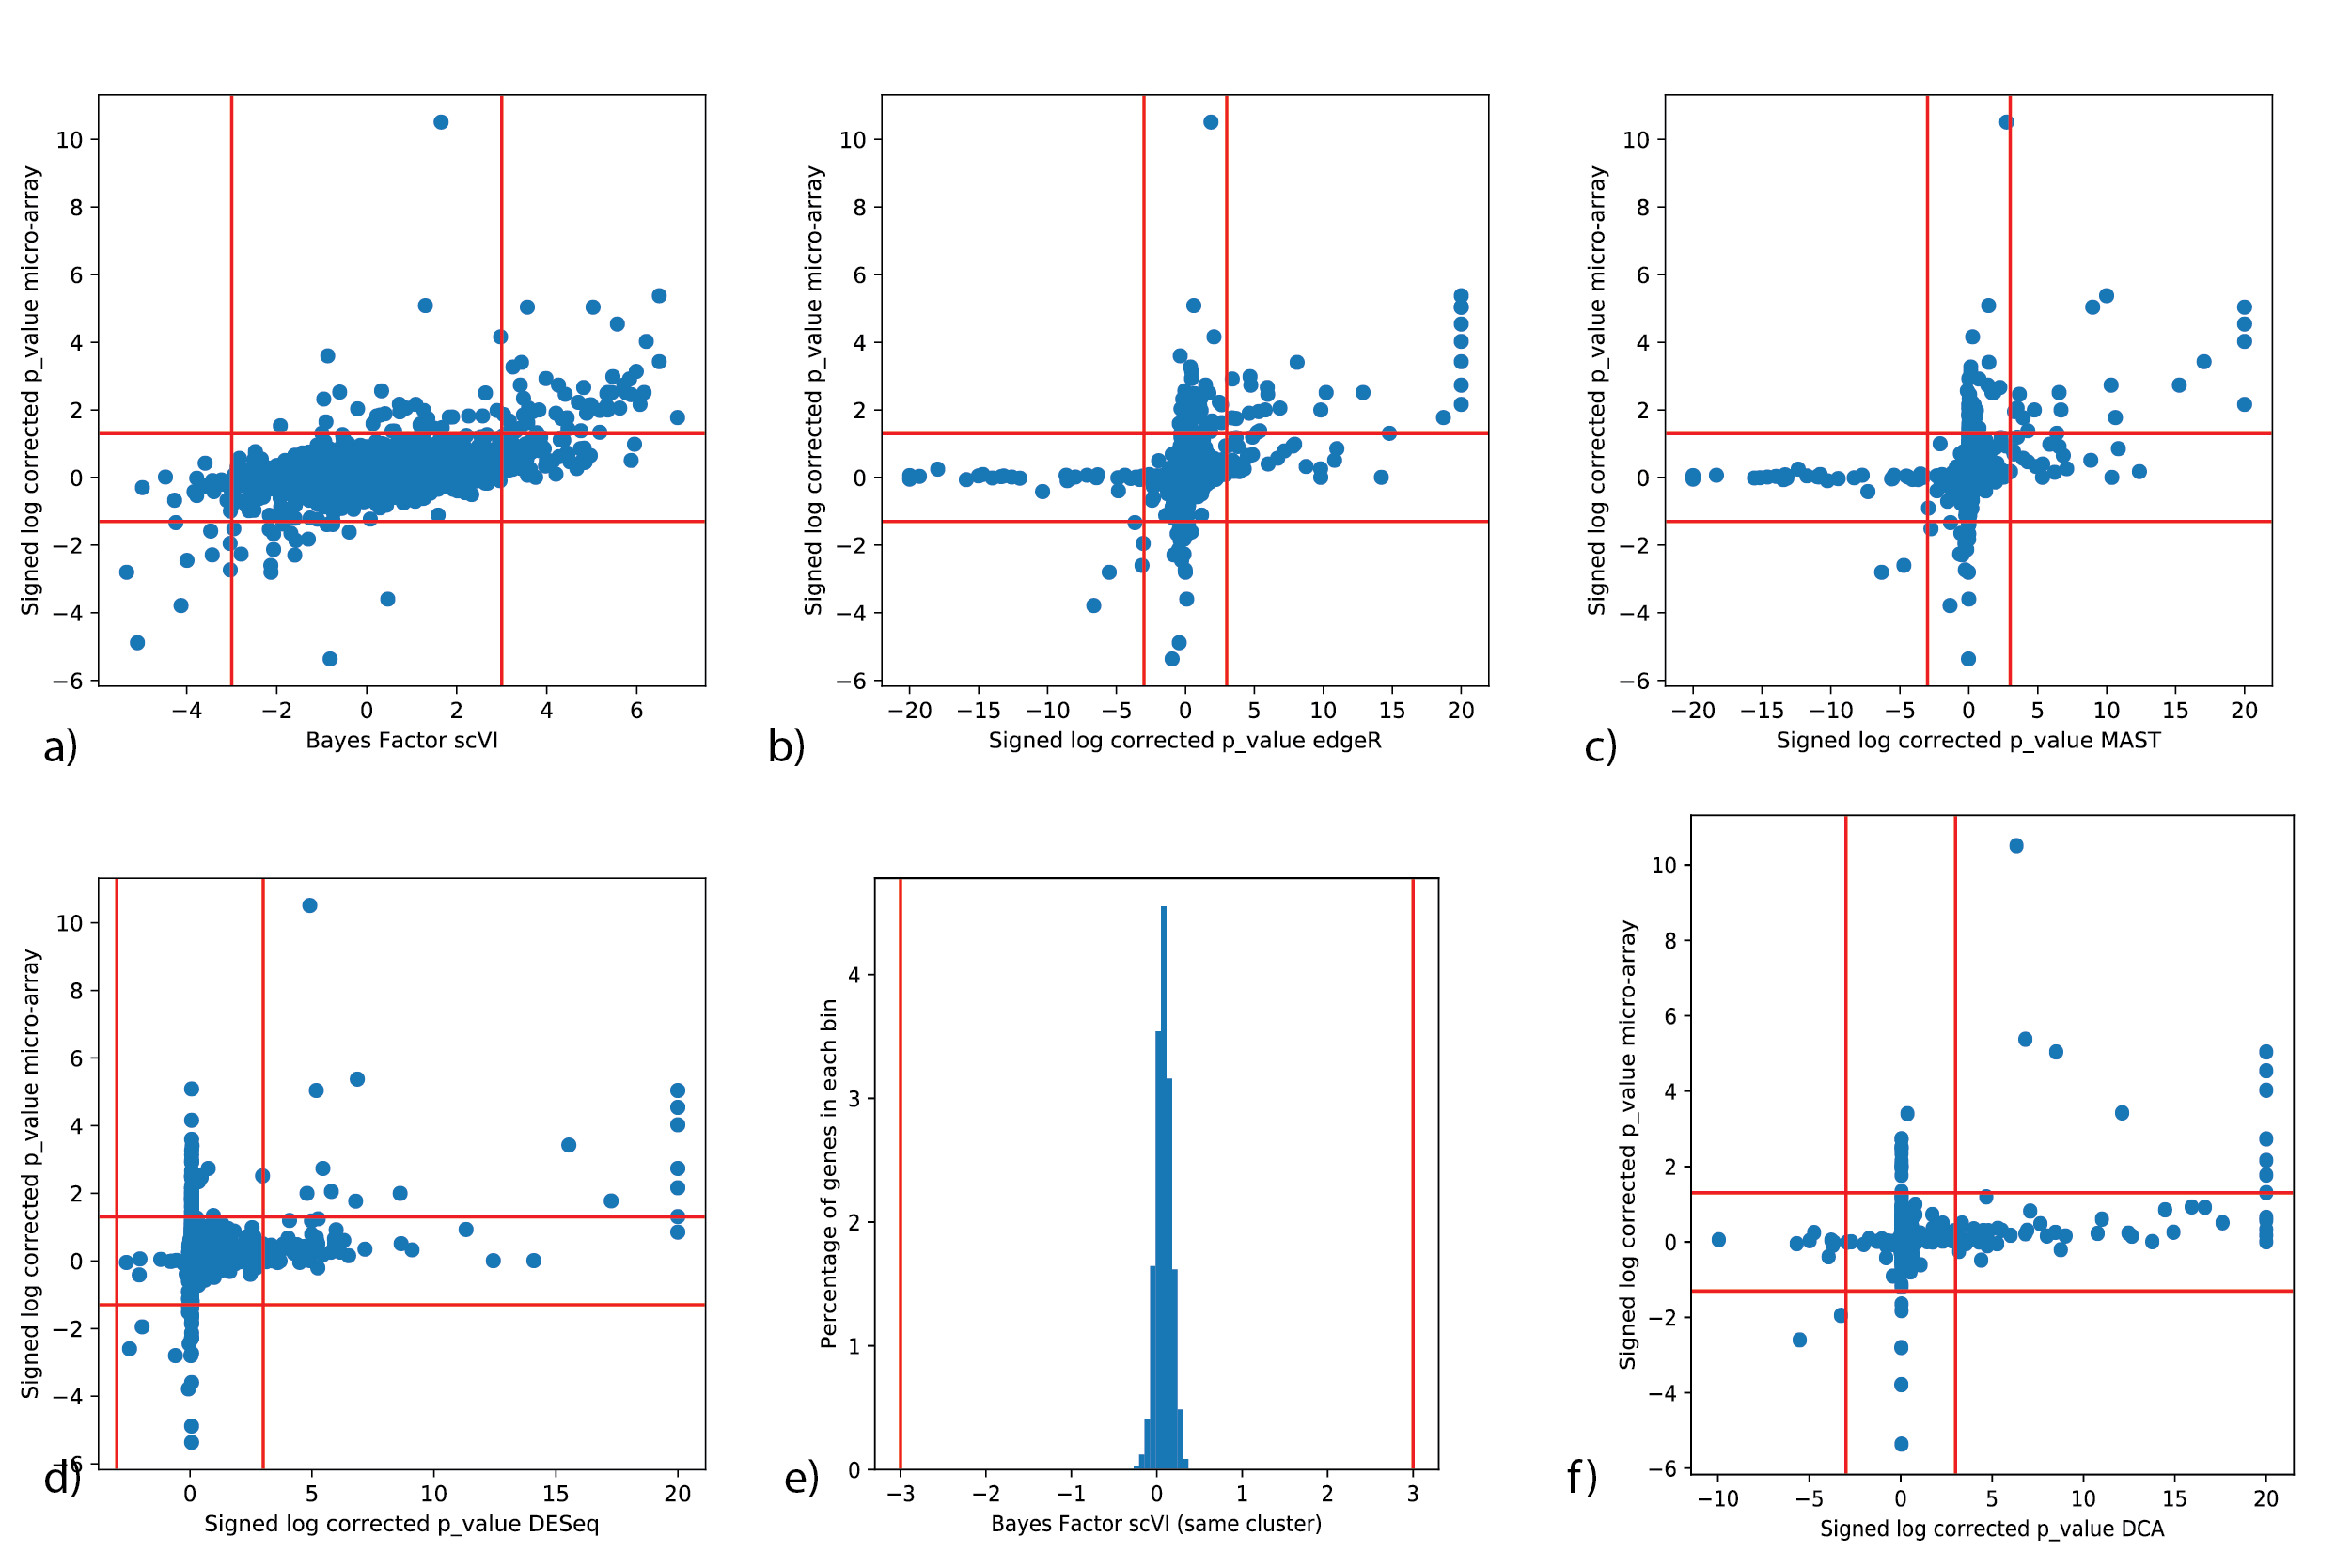
\includegraphics[width=\textwidth]{figures/de_figure.png}
\caption[Differential expression with scVI on the PBMC dataset]{Differential expression with scVI on the PBMC dataset. (a) (b) (c) (d) (f) p-values of microarray against p-values or Bayes factor for CD4 /CD8 comparison. In the order indicated, scVI, edgeR, MAST, DESeq2, DESeq2 on DCA imputed counts (e) Bayes factor of scVI when applying DE to two sets of random cells from the same cluster.}
\label{scvibayes_supp}
\end{suppfigure}

\begin{suppfigure}
\centering
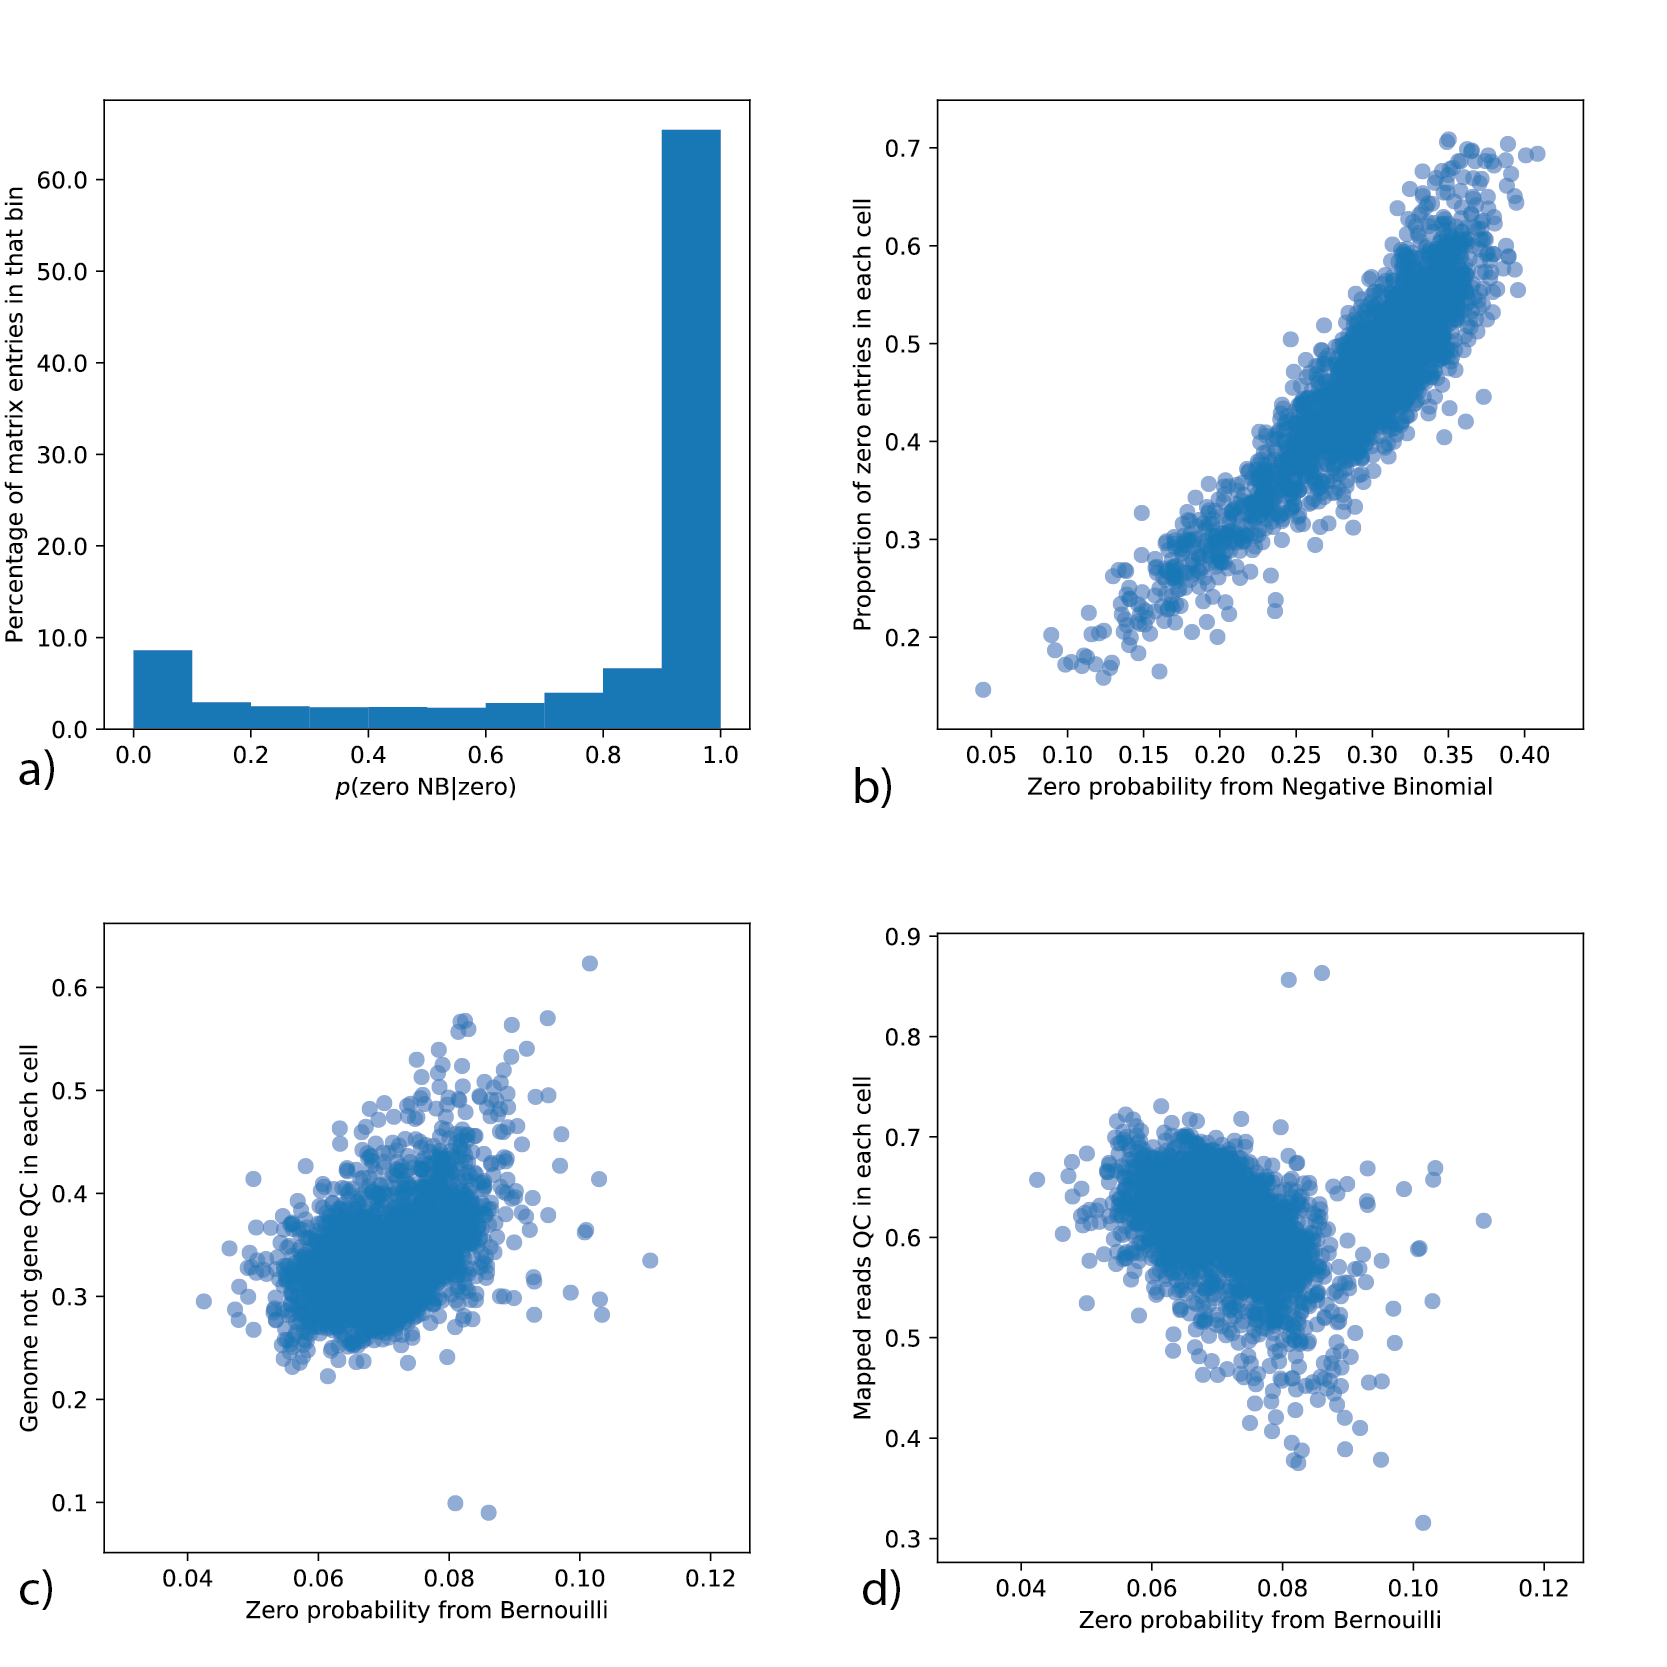
\includegraphics[width=\textwidth]{figures/parameter_supplement.png}
\caption[The generative distributions of scVI]{The generative distributions of scVI. This study focuses on a particular subpopulation of the BRAIN-SMALL dataset  ($n=2592$)
(a) To assess whether most of the zeros in the data comes from the negative binomial, for each entry of the count matrix (percentage in y-axis), we plot the probability that a given zero comes from the NB conditioned on having a zero (x-axis).
(b) Number of genes detected vs. negative binomial zero probability averaged across all genes.
(c) Genome\_not\_gene vs. Bernoulli zero probability averaged across all genes.
(d) Mapped\_reads vs. Bernoulli zero probability averaged across all genes. }
\label{scviparameters_supp}
\end{suppfigure}

\begin{suppfigure}
\centering
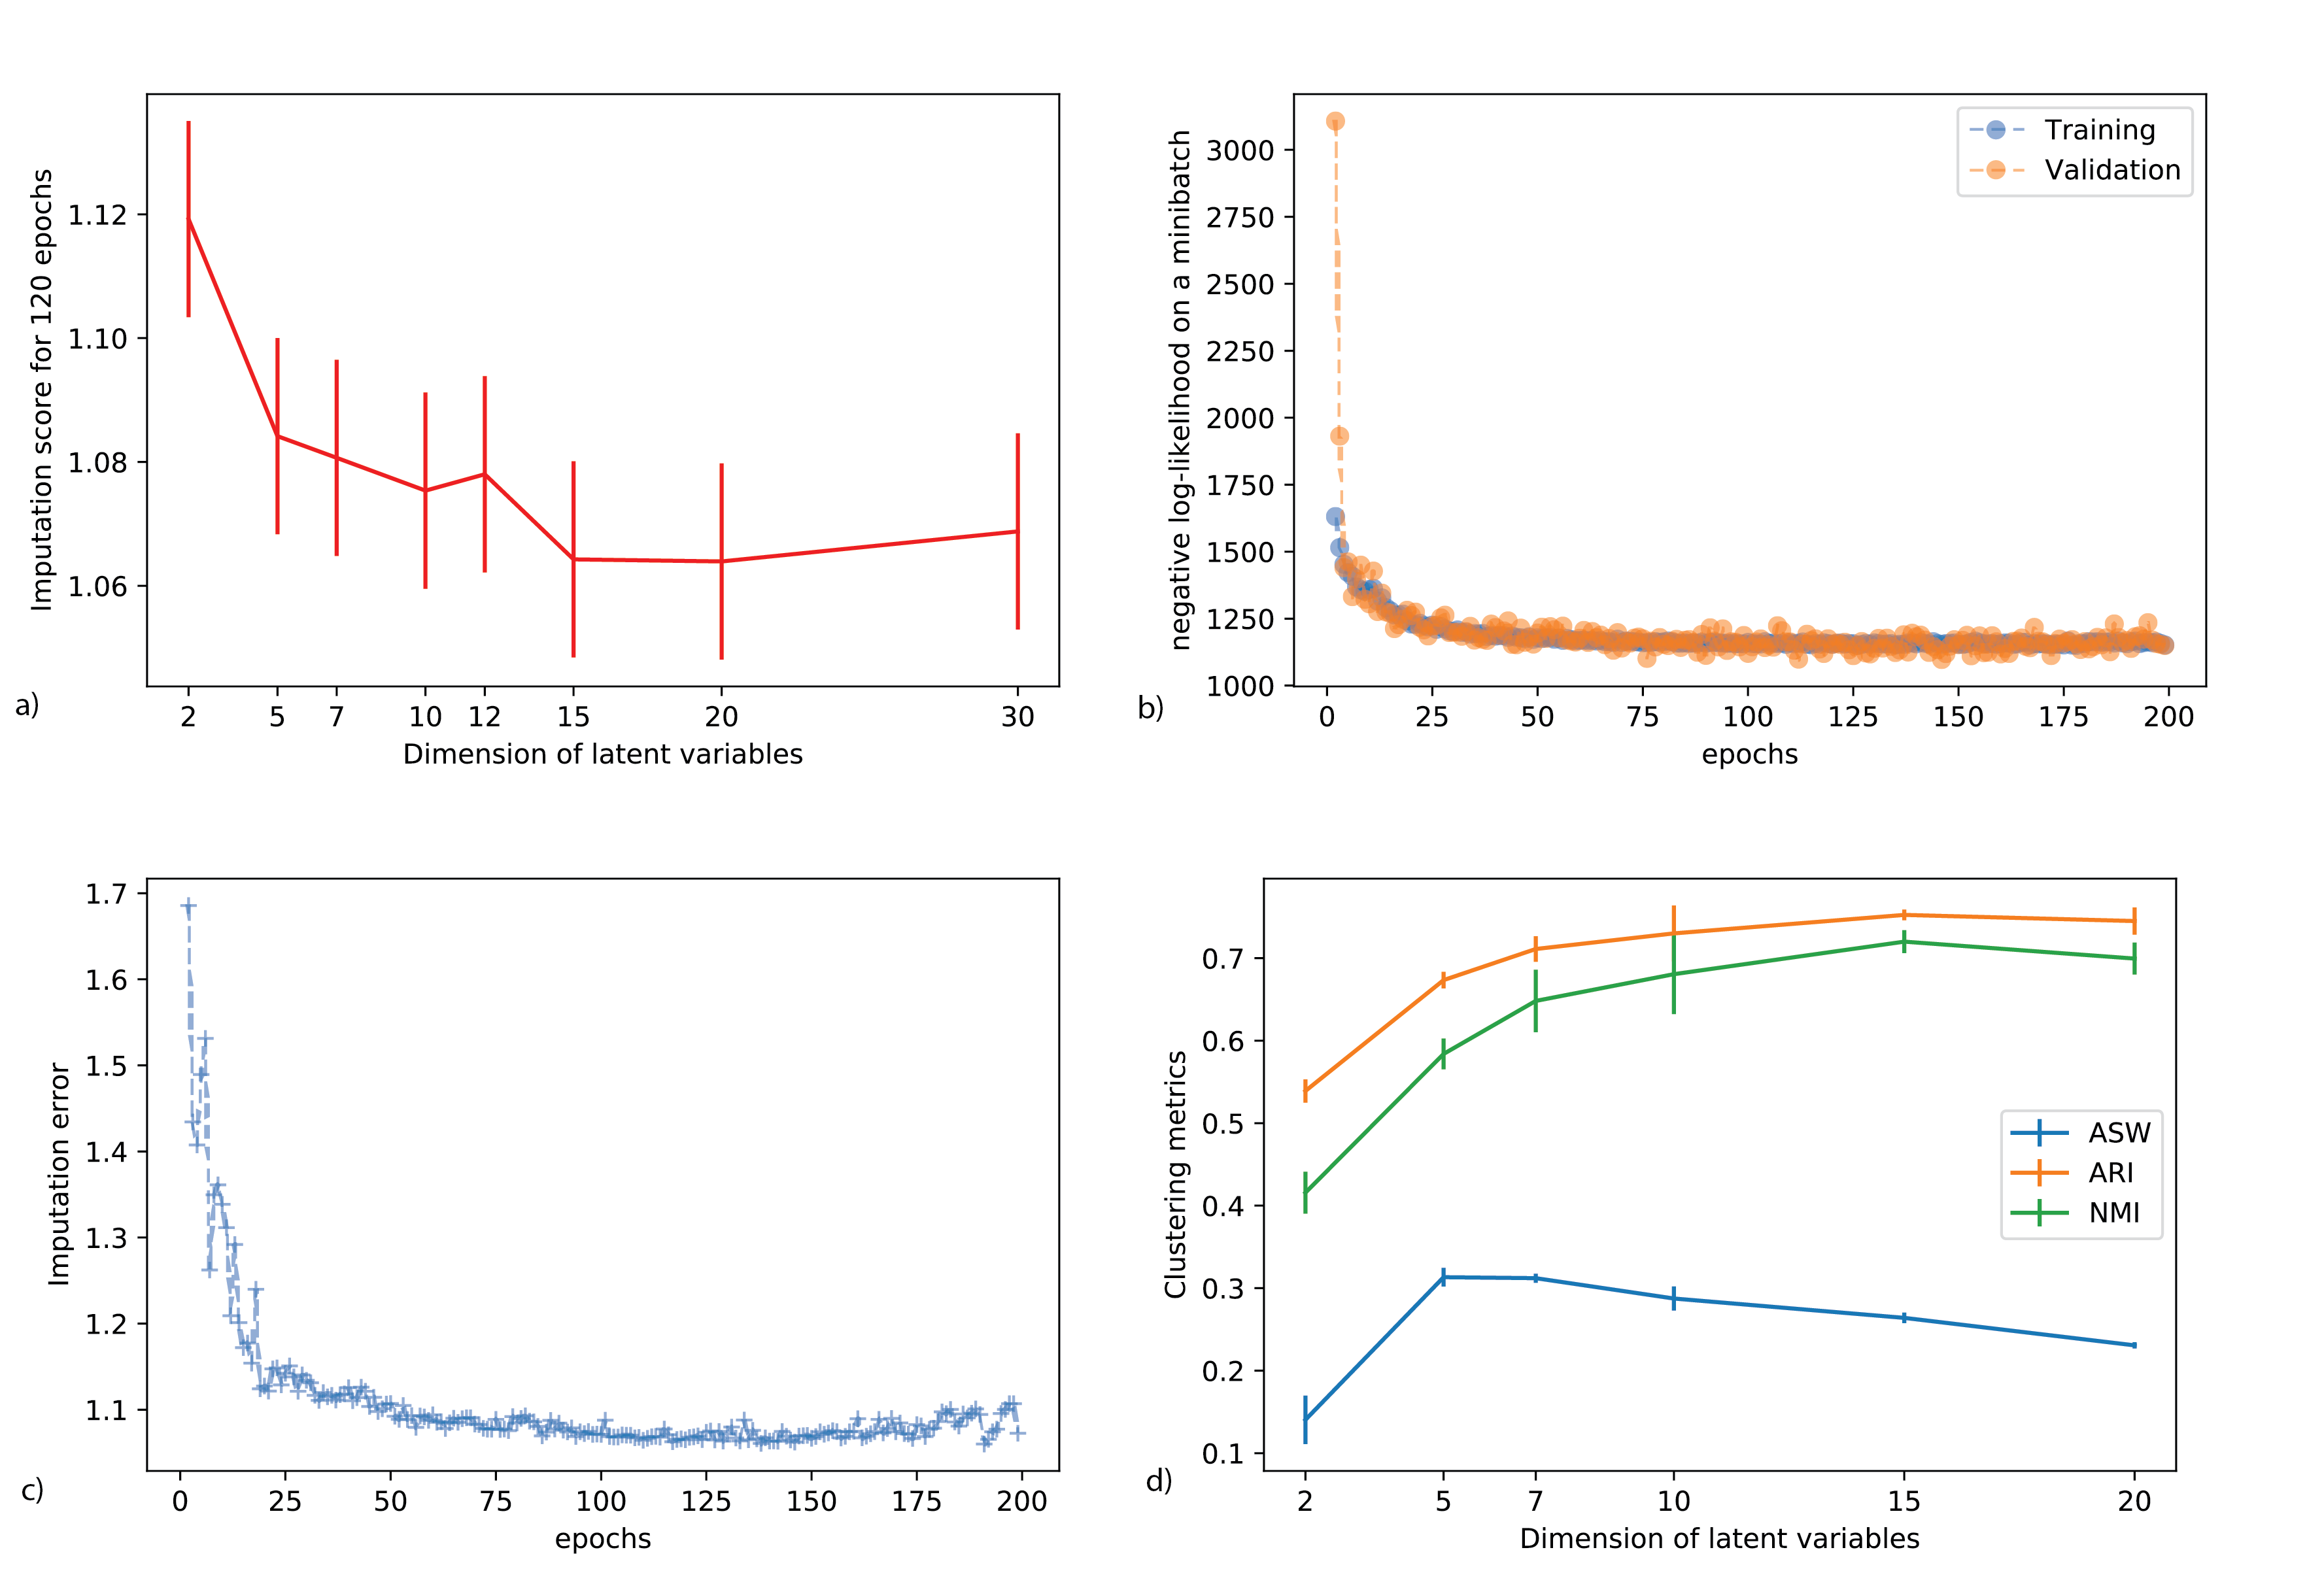
\includegraphics[width=\textwidth]{figures/stability_figure.png}
\caption[Robustness analysis for scVI]{Robustness analysis for scVI. Whiskers denote 5th and 95th percentiles. (a) Imputation score on the BRAIN-LARGE dataset across multiple random initialization, training and dimension of the latent space. (b) Visualization of scVI numerical objective function during training on the BRAIN-LARGE dataset. This shows our model does not over fit and has a stable training procedure. (c) Imputation score as a function of the number of epochs on the BRAIN-LARGE dataset. This figure also shows stability across posterior sampling since there is not much change in the parameters between two subsequent epochs. (d) Clustering metrics on the CORTEX dataset across multiple initializations and dimensions for the latent space.}
\label{scvirobustness}
\end{suppfigure}




\chapter{Harmonization and Annotation of Multiple Single-cell Experiments}
\chaptermark{Single-cell Annotation using Variational Inference}
\label{scanvi}
\section{Introduction}
Recent technological improvements in microfluidics and low volume sample handling~\cite{tanay2017scaling} have enabled the emergence of single-cell transcriptomics~\cite{dropseq, zheng2017massively} as a popular tool for analyzing biological systems~\cite{Semrau2017, Gaublomme2015, Patel2014}. This growing popularity along with a continued increase in the scale of the respective assays~\cite{angerer} has resulted in massive amounts of publicly available data and motivated large scale community efforts such as the Human Cell Atlas~\cite{HCA}, Tabula Muris~\cite{quake2018single} and the BRAIN Initiative Cell Census Network~\cite{biccn}. The next natural step in the evolution of this field is therefore to integrate many available datasets from related tissues or disease models in order to increase statistical robustness~\cite{boost}, achieve consistency and reproducibility among studies~\cite{MNN,seurat}, and ultimately converge to a common ontology of cell states and types~\cite{HCA, wagner2016revealing}. 

A fundamental step toward the ideal of a common ontology is data \textit{harmonization}, namely integration of two or more transcriptomics datasets into a single dataset on which any downstream analysis can be applied. We use the term harmonization rather than \textit{batch effect correction} in order to emphasize that the input datasets may come from very different sources (\textit{e.g.}, technology, laboratory), and from samples with a different composition of cell types. A wide range of methods have already been developed for this fundamental problem, initially for microarrays and later on for bulk RNA sequencing, such as ComBat~\cite{combat} and limma~\cite{limma}. These approaches mainly rely on generalized linear models, with empirical Bayes shrinkage to avoid over-correction. More recently, similar methods have been proposed specifically for single-cell RNA sequencing (scRNA-seq), such as ZINB-WaVE~\cite{zinbwave}, which explicitly accounts for the overabundance of zero entries in the data. However, because of their linear assumptions, these approaches may not be appropriate when provided with a heterogeneous sample that includes different cell states, each of which may be associated with a different sample-to-sample bias~\cite{MNN}. With these limitations in mind, the next generation of methods turned to non-linear strategies. Broadly speaking, each of these methods includes a combination of two components: (i) joint factorization of the input matrices (each corresponding to a different dataset) to learn a joint low-dimensional latent representation. This is usually done with well established numerical methods, such as integrative non-negative matrix factorization (LIGER~\cite{LIGER}), singular value decomposition (Scanorama~\cite{scanorama}), or canonical correlation analysis (Seurat Alignment~\cite{seurat}); (ii) additional non-linear transformation of the resulting latent representations so as to optimally ``align'' them onto each other. This is usually done using heuristics, such as alignment of mutual nearest neighbors (MNN~\cite{MNN}, Scanorama~\cite{scanorama} and Seurat Anchors~\cite{SEURAT3}), dynamic time warping (Seurat Alignment~\cite{seurat}) or quantile normalization (LIGER~\cite{LIGER}). While this family of methods has been shown to effectively overlay different datasets, it suffers from two important limitations. First, an explicit alignment procedure may be difficult to tune in a principled manner and consequently result in over-normalization. This is especially relevant when the cell type composition is different between datasets and when technical differences between samples are confounded with biological differences of interest. Second, the alignment is done in an ad hoc manner and lacks probabilistic interpretability. Consequently, the resulting harmonized dataset is of limited use and cannot be directly applied for probabilistic decision-making tasks, for example differential expression. 


Besides harmonization, another important and highly related problem is that of automated \textit{annotation} of cell state. In principle, there are two ways to approach this problem. The first is \textit{ab initio} labeling of cells based on marker genes or gene signatures \cite{seurat,VISION,fastproject}. While this approach is intuitive and straightforward, its performance may be affected in the plausible case where marker genes are absent due to limitations in sensitivity. The second approach is to ``transfer'' annotations between datasets. In the simplest scenario, we have access to one dataset where states have been annotated either \textit{ab initio}, or using additional experimental measurements (e.g., protein expression~\cite{zheng2017massively, stoeckius2017simultaneous} or lineage tracing~\cite{Weinreb467886}) and another, unannotated dataset from a similar condition or tissue. The goal is to use the labeled data to derive similar annotations for the second dataset, whenever applicable. This task is often complicated by factors such as differences in technology (e.g., using Smart-Seq2 data to annotate 10x Chromium data), partial overlap in cell type composition (i.e., not all labels should be transferred and not all unannotated cells should be assigned a label), complex organization of the labels (e.g., hierarchy of cell types and sub-types~\cite{Moana}, continuum along phenotypic or temporal gradients), partial labeling (i.e., only a subset of cells from the ``annotated'' dataset can be assigned a label confidently), and the need to handle multiple (more than $2$) datasets in a principled and scalable manner. One way to address the annotation problem with this approach is  learning a classifier~\cite{Moana, scmap} in order to predict a fixed stratification of cells. However, this approach might be sensitive to batch effects, which could render a classifier based on a reference dataset less generalizable to an unannotated dataset. Another, more flexible approach is to transfer annotations by first harmonizing the annotated and unannotated datasets, thus also gaining from the benefits of having a single dataset that can be subject to additional, joint, downstream analysis.

In this chapter, we propose a strategy to address several of the outstanding hurdles in both of the harmonization and annotation problems. We first demonstrate that single-cell Variational Inference (scVI)~\cite{scvi} a deep generative model we previously developed for probabilistic representation of scRNA-seq data --- performs well in both harmonization and harmonization-based annotation, going beyond its previously demonstrated capacity to correct batch effects. We then introduce single-cell ANnotation using Variational Inference (scANVI), a new method that extends scVI and provides a principled way to address the annotation problem probabilistically while leveraging any available label information. Because scANVI is able to model cells with or without label information, it belongs to the category of semi-supervised learning algorithms. This flexible framework of semi-supervised learning can be applied to two main variants of the annotation problem. In the first scenario, we are concerned with a single dataset in which only a subset of cells can be confidently labeled (e.g., based on expression of marker genes) and annotations should then be transferred to other cells, when applicable. In the second scenario, annotated datasets are harmonized with unannotated datasets and then used to assign labels to the unannotated cells.

The inference procedure for both of the scVI and scANVI models relies on neural networks, stochastic optimization and variational inference~\cite{aevb,VFAE} and scales to large numbers of cells and datasets. Furthermore, both methods provide a complete probabilistic representation of the data, which non-linearly controls not only for sample-to-sample bias but also for other technical factors of variation such as over-dispersion, library size discrepancies and zero-inflation. As such, each method provides a single probabilistic model that underlies the harmonized gene expression values (and the cell annotations, for scANVI), and can be used for any type of downstream hypotheses testing. We demonstrate the latter point through a differential expression analysis on harmonized data. Furthermore, through a comprehensive analysis of performance in various aspects of the harmonization and annotation problems and in various scenarios, we demonstrate that scVI and scANVI compare favorably to current state-of-the-art methods. scANVI is publicly available at \url{https://github.com/YosefLab/scvi-tools}. An implementation for all of the analysis performed in this chapter is available at
\url{https://doi.org/10.5281/zenodo.2529945}.





\section{Overview of our proposed probabilistic models for harmonization}

%%%%%%%%%%%%%%%%%%%%%%%%%%%%%%%%%%%%%%%%%%%%%%%%%%%%%%
\subsection{Joint modeling of scRNA-seq datasets}
%%%%%%%%%%%%%%%%%%%%%%%%%%%%%%%%%%%%%%%%%%%%%%%%%%%%%%
We consider a collection of scRNA-seq datasets (Figure~\ref{scanviscanvi_presentation}ab). After using a standard heuristic to filter the genes and generate a common (possibly large) gene set of size $G$, we obtain a concatenated dataset that may be represented as a matrix. Individual entries $x_{ng}$ of this matrix measures the expression of gene $g$ in cell $n$. Additionally, we use the integer $s_n$ to denote the dataset of origin for each cell $n$. Finally, a subset of the cells may be associated with a cell state annotation $c_n$, which can describe either discrete cell types or hierarchical cell types. More complex structures over labels such as gradients are left as a future research direction. 

Since the problem of data harmonization of single-cell transcriptomics is difficult and can potentially lead to over-correction~\cite{batchfalsede}, we propose a fully-generative method as a robust and principled approach to address it. In our previous work~\cite{scvi}, we built single-cell Variational Inference (scVI), a deep generative model where the expression level $x_{ng}$ is zero-inflated negative binomial (ZINB) when conditioned on the dataset identifier ($s_n$), and two additional latent random variables. The first, which we denote by $l_n$, is a one-dimensional random variable accounting for the variation in capture efficiency and sequencing depth. In practice, we noticed that this random variable is highly correlated to the library size~\cite{scvi}. The second, which we denote as $z_n$, is a low dimensional random vector that represents the remaining variability~(Figure~\ref{scanviscanvi_presentation}b). This vector is expected to reflect biological differences between cells, and can be effectively used for visualization, clustering, pseudotime inference and other tasks. Since the scVI model explicitly conditions on the dataset identifier (in the sense that it learns a conditional distribution), it provides an effective way of controlling for technical sample-to-sample variability. However, scVI is unsupervised and does not make use of the available annotations $c_n$, which can further guide the inference of an informative latent representation $z_n$. To this end, we present a more refined hierarchical structure for $z_n$. We draw $z_n$ as a mixture conditioned on the cell annotation $c_n$ and another latent variable $u_n$, accounting for further biological variability within a cell type. We name the resulting approach single-cell ANnotation using Variational Inference (scANVI). 

The variables $z_n$, inferred either with scVI or scANVI, provide an embedding of all cells in a single, joint latent space. Since this latent space is inferred while controlling for the dataset of origin ($s_n$), it inherently provides a way to address the harmonization problem. The annotation of unlabeled cells can therefore be conducted with scVI using their proximity to annotated cells in the joint latent space (e.g., using majority vote over the $k$-nearest neighbors). The scANVI model provides a more principled way to annotate cells, namely through a Bayesian semi-supervised approach. Once fitted, the model is able to provide posterior estimates for the unobserved cell state $c_n$, which can be particularly useful when labels cannot be entirely trusted. 


\begin{figure}
\centering
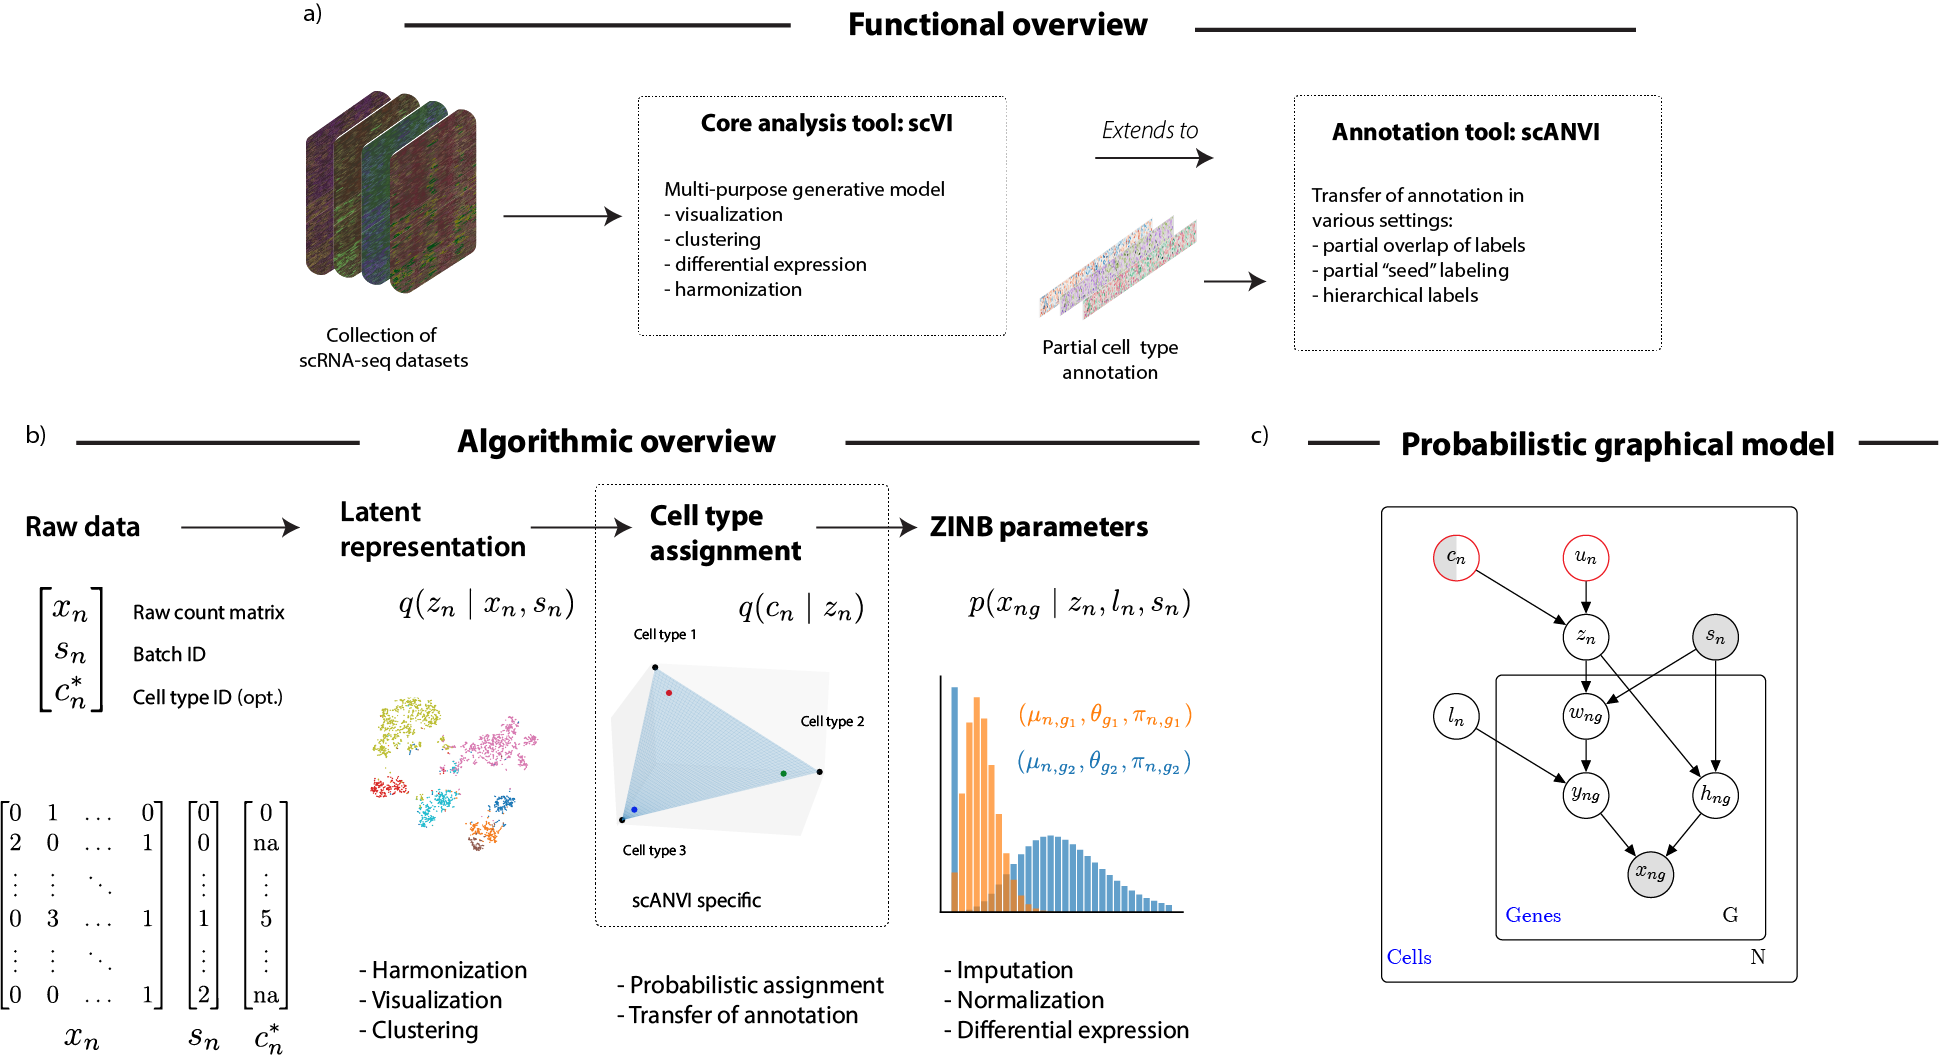
\includegraphics[width=\textwidth]{figures/Figure1.png}
\caption[Harmonization and annotation of scRNA-seq datasets with generative models]{Harmonization and annotation of scRNA-seq datasets with generative models. $(a)$ Functional overview of the methods proposed in this chapter. $(b)$ Schematic diagram of the variational inference procedure in both of the scVI and scANVI models. We show the order in which random variables in the generative model are sampled and how these variables can be used to derive biological insights. $(c)$ The graphical models of scVI and scANVI. Vertices with black edges represent variables in both scVI and scANVI, and vertices with red edges are unique to scANVI. Shaded vertices represent observed random variables. Semi-shaded vertices represent variables that can be either observed or random. Empty vertices represent latent random variables. Edges signify conditional dependency. Rectangles (``plates'') represent independent replication.}.
\label{scanviscanvi_presentation}
\end{figure}


\subsection{Definition of the generative model for scANVI}

In our generative model, we assume each cell $n$ is an independent realization of the following generative process. Let $K$ be the number of datasets and $C$ be the number of cell types across all datasets (including cell types that are not observed). Let $\mathbf{c}$ describe the expected proportion of cells for each cell type. As in general this information is not available to the user, we consistently use a non-informative prior $\mathbf{c} = \nicefrac{1}{C}$ in the chapter. Although some prior information about proportions of cell type is generally accessible, we observe that using the non-informative prior allows us to recover the correct proportion of cells. In addition, in comparative studies such as disease case-control comparisons, or between tissue comparisons of immune cells \cite{schafflick2019ms} we might not want to bias the estimate of cell-type proportion by prior knowledge. All in all, adjustment of the prior $\mathbf{c}$ is not required.  Latent variable 
\begin{align}
c_n \sim  \mathrm{Multinomial}(\mathbf{c}),
\end{align}
describes the cell type of the cell $n$. Latent variable  
\begin{align}
    u_n \sim \mathcal N(0, I),
\end{align}
is a low-dimensional random vector describing cell $n$ within its cell type. Conceptually, this random variable could describe cell-cycles or sub-cell types. By combining cell type information $c_n$ and random vector $u_n$, we create a new low-dimensional vector
\begin{align}
    z_n  \sim \mathcal{N}(f^{\mu}_{z} (u_n, c_n), f^{\sigma}_{z} (u_n, c_n)),
\end{align}
where $f^{\mu}_{z}$ and $f^{\sigma}_{z}$ are two functions parametrized by neural networks. Let $s_n$ encode the dataset information. Given $l_\mu \in \mathbb{R}_+^K$ and $l_\nu \in \mathbb{R}_+^K$ specified per dataset as in~\cite{scvi}, latent variable
\begin{align}
    l_n \sim \textrm{LogNormal}(l^{s_n}_\mu, l^{s_n}_\nu),
\end{align} 
encodes a cell-specific scaling factor. As the prior are adjusted per dataset, our inference procedure will shrink the posteriors towards dataset specific values. This is particularly useful when aligning datasets with dramatically different library size values. Let $\theta \in \mathbb{R}_+^G$ encode a gene specific inverse dispersion parameter (inferred as in~\cite{scvi}). Conditional distribution $x_{ng} \mid z_n, l_n, c_n, s_n$ is conform to the one from the scVI model
\begin{align}
w_{ng} &\sim \mathrm{Gamma}(f^g_w(z_n, s_n), \theta_g)\\
y_{ng} &\sim \mathrm{Poisson}(l_nw_{ng})\\
h_{ng} &\sim \mathrm{Bernoulli}(f^g_h(z_n, s_n))\\
x_{ng} &=
\begin{cases}
y_{ng} & \text{ if } h_{ng} = 0\\
0 & \text{ otherwise}\\
\end{cases},
\end{align}

where $f_w$ and $f_h$ are functions parametrized by neural networks. $f_w$ has a final softmax layer to represent normalized expected frequencies of gene expression as in~\cite{scvi}. Let us note that the resulting distribution for the counts is zero-inflated negative binomial. However, it is straightforward using our implementation to use a negative binomial or a Poisson noise model instead. In this model, annotation $c_n$ can be either observed or unobserved following~\cite{VFAE, m1m2}, which is useful in our applications where some datasets would come partially labeled or unlabeled. Only the first part of the generative model, as separated above, differs from the original scVI formulation. This corresponds to the top part of the new representation of the graphical model in Figure~\ref{scanviscanvi_presentation}b. 



\subsection{Variational inference recipe}

We rely on collapsed variational inference, a standard approximate Bayesian inference procedure that consists in analytically integrating over some of the random variables~\cite{NIPS2006_3113} before optimizing the parameters. As we proved in~\cite{scvi}, we can integrate the random variables $\{ w_{ng}, y_{ng}, h_{ng} \}$ to simplify our model at the price of a looser though tractable lower bound ($x_{ng} \mid z_n, l_n, s_n$ is zero-inflated negative binomial). This procedure reduces the number of latent variable and avoids the need for estimating discrete random variables, which is a harder problem. We then use variational inference, neural networks and the stochastic gradients variational Bayes estimator~\cite{aevb} to perform efficient approximate inference over the latent variable $\{ z_n, u_n, c_n, l_n\}$. We assume our variational distribution factorizes as:
\begin{align}
q_\Phi(c_n, z_n, l_n, u_n \mid x_n, s_n) = q_\Phi(z_n \mid x_n)q_\Phi(c_n \mid z_n)q_\Phi(l_n \mid x_n)q_\Phi(u_n \mid c_n, z_n).
\end{align}

Following~\cite{VFAE, m1m2}, we derive two variational lower bounds: one $\mathcal{L}$ in the case of $c_n$ observed for $p_\Theta(x_n, c_n \mid s_n)$ and a second $\mathcal{U}$ in the case of $c_n$ non-observed for $p_\Theta(x_n \mid s_n)$ where $\Theta$ are all the parameters (neural networks and inverse-dispersion parameters). 

We derive the \emph{evidence lower bound} (ELBO) and detail the training details in the following notes. Briefly, we optimize the sum $\text{ELBO} = \mathcal{L} + \mathcal{U}$ over the neural networks parameters and the inverse-dispersion parameters (in a variational Bayesian inference fashion). Remarkably, the approximate posterior $q_\Phi(c_n \mid z_n)$ can be used as a classifier, assigning cells to cell types based on the location on the latent space. 

We sample from the variational posterior using the reparametrization trick~\cite{aevb} as well as ``mini-batches'' from the dataset to compute unbiased estimate of the objective gradients' with respect to the parameters. We use Adam~\cite{adam} as a first-order stochastic optimizer to update the model parameters. 

\subsubsection{Evidence Lower Bound decomposition}
We drop the parameters $\Theta$ (resp. $\Phi$) of the generative model (resp. the variational distribution) for notational convenience, as well as the conditioning on the batch identifier $s$. We report the evidence lower bound (ELBO) only for one sample (i.e one cell) and drop the index notations by substituting $\{x_n, z_n, u_n, c_n, l_n\}$ by $\{x, z, u, c, l\}$. This is without loss of generality since all the cells are independent and identically distributed under our model.

We derive the ELBO in the case where $c$ is not observed (almost same calculations resolve the case where $c$ is observed). Similar derivations can be found in the variational autoencoder literature~(e.g, \cite{m1m2}). We assume our variational distribution factorizes as:
\begin{align}
    q(c, z, u, l \mid x) = q(z \mid x)q(c \mid z)q(u \mid z, c)q(l \mid x).
\end{align}
In this case, we may simply apply Jensen's inequality weighted by the variational distribution~$q(z, u, l, c \mid x)$:
\begin{align}
    \log p(x) &\geq \Elog{\qall}{\frac{p(x, z, u, c, l)}{\qall}} \\
    &= \Elog{\qall}{\frac{p(x \given z, l)p(z \given u, c)p(c)p(u)p(l)}{\qall}}.
\end{align}
Then, by decomposing this last term, we obtain the following lower bound:
\begin{align}
\begin{split}
    \log p(x) & \geq \underbrace{\Elog{\qall}{p(x \given z, l)}}_{\text{\emph{(i)}}} + \underbrace{\Elog{\qall}{\frac{p(z \given u, c)}{q(z \given x)}}}_{\text{\emph{(ii)}}} \\
    & \qquad + \underbrace{\Elog{\qall}{\frac{p(c)}{q(c \given z)}}}_{\text{\emph{(iii)}}}+ \underbrace{\Elog{\qall}{\frac{p(u)}{q(u \given z,c)}}}_{\text{\emph{(iv)}}} \\
    & \qquad + \underbrace{\Elog{\qall}{\frac{p(l)}{q(l \given x)}}}_{\text{\emph{(v)}}}
\end{split}
\label{scanvielbo}
\end{align}
Then we simplify each individual term of the ELBO in \ref{scanvielbo} by recognizing KL divergence terms. In particular, we use subscript notation $\KLG{.}{.}$, and $\KLM{.}{.}$ to denote Gaussian and multinomial KL divergences.
\begin{align}
    \Elog{\qall}{p(x \given z, l)} &= \Elog{q(z \given x)q(l \given x)}{p(x \given z, l)} \tag{i}\\
    \Elog{\qall}{\frac{p(z \given u, c)}{q(z \given x)}} &= \E{q(z \given x)}{\Elog{q(u \given z,c)q(c \given z)}{\frac{p(z \given u, c)}{q(z \given x)}}} \tag{ii}\\
&= \E{q(z\given x)}{\sum_{c=1}^K q(c \given z) \Elog{q(u \given z,c)}{\frac{p(z \given u, c)}{q(z \given x)}}} \notag \\
    \Elog{\qall}{\frac{p(c)}{q(c \given z)}} &= \E{q(z \given x)}{ \underbrace{\sum_{c=1}^K q(c \given z) \log \frac{p(c)}{q(c \given z)}}_{-\KLM{q(c \given z)}{p(c)}} } \tag{iii}\\
    \Elog{\qall}{\frac{p(u)}{q(u \given z,c)}} &= \E{q(z \given x)}{ \sum_{c=1}^K q(c \given z) \underbrace{\Elog{q(u \given z, c)}{ \frac{p(u)}{q(u \given z, c)}}}_{-\KLG{q(u \given z, c)}{p(u)}} } \tag{iv}\\
    \Elog{\qall}{\frac{p(l)}{q(l \given x)}} &= -\KLG{q(l \given x)}{p(l)}  \tag{v}
\end{align} 


\subsection{Customized training procedures}
In order to train scANVI properly, several options are possible to train all the parameters ($\theta$ from the generative model, $\phi$ from the variational distribution except the labels' posterior and $\phi^{\mathcal{C}}$ from the labels' posterior exclusively). In all cases, parameters $\theta$ and $\phi$ should minimize the evidence lower bound 
\begin{align}
    \mathcal{J} = \mathcal{L} + \mathcal{U},
\end{align}
decomposed over the labeled samples $\mathcal{L}$ and unlabeled samples $\mathcal{U}$. Furthermore,~\cite{m1m2} suggests to jointly optimize a modified objective that penalize the ELBO by a classification loss $\mathcal{C}$ on the labeled data so that the parameters $\phi^{\mathcal{C}}$ also benefits from the learned data. They introduce the modified objective function 
\begin{align}
\mathcal{J}_{\alpha} = \mathcal{J} + \alpha \cdot \mathcal{C},
\end{align}
where $\alpha$ is a parameter set by cross-validation. This modified lower bound can be interpreted as placing a Dirac prior on $c$~\cite{m1m2} or as a correction term for noisy labels~\cite{noisylabels}. In their procedure, $\mathcal{J}_\alpha$ is optimized with respect to all parameters $[\theta, \phi, \phi^{\mathcal{C}}]$ and for a fixed number of epochs. This joint training procedure is appealing as it shapes the latent space directly, through the modification of the encoder’s weights. However, we found this approach to have two limitations. First, this joint training breaks down the mixing in the latent space in the case of transferring labels from one dataset to another. We attribute this to the loss $\mathcal{C}$ having only contributions from a unique dataset. Second, we did not find convenient to choose the optimal value for the parameter $\alpha$ and concluded it may not be desirable for a practitioner either. 

We use in scANVI an alternate training procedure which deletes the need for $\alpha$ and has better performance in the setting of transferring annotations. We aggressively train the classifier separately, updating the parameters $\phi^\mathcal{C}$ for $c > 1$ epochs for every single epoch of updating $[\theta, \phi]$. The total number of epochs is fixed and chosen high enough to guarantee convergence. In the case of a single dataset (resp. transfer of labels), we use $c=1$ (resp. $c=100$) epochs of classifier training in between each variational update. This helps the classifier correctly identify cell types at the end of each epoch of updating $\phi^\mathcal{C}$. This is a clearly advantageous procedure, because it then improve indirectly the latent space quality, through the next steps of optimization. 




\subsection{Choice of hyperparameters}

Notably, scANVI and scVI both have a certain number of hyperparameters. In the following evaluations, conducted on different datasets and different scenarios, we use the exact same set of hyperparameters in order to demonstrate that our methods can be applied with a minimal requirement of hyperparameter tuning. 

For all harmonization tasks in this chapter, we consistently use the same set of hyperparameters. Each network has exactly 2 fully-connected layers, with 128 nodes each. The number of latent dimensions is 10, the same as other algorithms for benchmarking purposes (e.g., the number of canonical correlation vectors used in Seurat Alignment). The activation functions between two hidden layers are all ReLU. We use a standard link function to parametrize the distribution parameters (exponential, logarithmic or softmax). Weights for the first hidden layer are shared between $f_w$ and $f_h$. We use Adam with $\eta = 0.001$ and $\epsilon = 0.01$. We use deterministic warmup~\cite{warmup} and batch normalization~\cite{batchnorm} in order to learn an expressive model. When we train scANVI, we therefore assume that the data come from a set of $C_\text{observed}+C_\text{unobserved}$ populations, each generated by a different distribution of $z_n$ values. This set includes the $C_\text{observed}$ populations for which annotated cells are available, and $C_\text{unobserved}$ population that accounts for cell types for which an annotation is not available to the algorithm. 

We also provide a robustness study for hyperparameters in the context of harmonization in Figure~\ref{scanvirobustness_supplement}. 

\subsection{Alternative model choices}

\subsubsection{Zero-inflation in the context of harmonization}
 In this chapter, we mainly rely on a zero-inflated negative binomial (ZINB) distribution for the counts --- which is a widely used model for single cell transcriptomics data. Recent research however suggests that for some technologies such as droplet-based UMI single-cell protocols, the abundance of zero mainly may be explained only by limited sensitivity and subsampling effect \cite{svensson2019droplet}. On the other hand, zero-inflated might be a realistic addition to count distributions for describing full-length plate-based technologies data \cite{vieth2017powsimr}. Indeed, it has been hypothesized that PCR duplication or uneven fragment sampling may be responsible for zero-inflation in plate-based technologies \cite{svensson2019droplet}. Still, no definite conclusion can be drawn about which distribution better fits UMI technologies or full-length method. Although full-length methods seem more affected by technical noise, they also provide extra information at the transcript resolution that is lost in droplet-based UMI methods. Consequenly, many consortia have chosen to obtain data by both full-length and UMI methods~\cite{quake2018single,ecker2017brain}. A method that can flexibly use different distribution and appropriately these two data types is therefore extremely valuable for analyzing collections of single cell transcriptomics data. 
 
 scVI and scANVI are both flexible to use both ZINB and NB methods and we show in Figure~\ref{scanviZINB_NB} that the benchmarking results are similar using both methods in all four datasets used in our benchmarking procedure. However, we observed that for MarrowTM dataset, using the ZINB version of scVI does perform better in terms of harmonization. Since in this case, we are merging a 10x dataset with a Smart-Seq2 dataset, we compared the average zero-inflation parameter for each gene in each dataset and found that the differences between Smart-Seq2 and 10x are significantly skewed to the right (more zero-inflation in Smart-Seq2, $p$=6.3e-31, using a D'Agostino-Pearson $K^2$ test). Finally, we also performed differential expression with negative binomial versions of scVI and scANVI and show that results are similar (Figure~\ref{scanviDE_NB}). These results show that both NB and ZINB model can be used in scVI and scANVI and in most instances, downstream analysis might not be impacted by this modeling choice. Interestingly, our model successfully learns the difference in the degree of zero-inflation in different datasets while merging them and exploits this information when necessary.
 
 
 \subsubsection{Library-size prior for scVI and scANVI}
 Besides zero-inflation, another major difference between sequencing technologies is the sequencing depth. scVI and scANVI both make use of technical scalar factors that have a batch-specific prior, and are therefore extremely suited for this setting. 
 To evaluate the effectiveness of both the model and the prior choice, we compute the negative log likelihood of the scVI model using ZINB with batch-specific library size prior, ZINB with shared library size prior, NB with a batch-specific library size prior, and NB with shared library size prior. All four models are fit on two pairs of datasets, DentateGyrus (Fluidigm C1 and 10x) and MarrowTM (10x and SmartSeq2). Since only the second pair is a comparison between UMI and full-length datasets, we expect the differences between the four model choices to be larger in the MarrowTM comparison, and that ZINB with batch-specific library size prior to have the highest likelihood (reported in Table~\ref{library_size_ll}). 

\begin{table}
\centering
\begin{small}
\begin{tabular}{lcc}
    \toprule
\textbf{Negative log-likelihood}           & \textbf{DentateGyrus} & \textbf{MarrowTM} \\
\midrule
\textbf{ZINB model / batch-specific prior}                        & 514.5        & 2339.8   \\
\textbf{ZINB model / shared prior}  & 513.8        & 2349.2   \\
\textbf{NB model / batch-specific prior}                         & 523.4        & 2531.3   \\
\textbf{NB model / shared prior}   & 524.0        & 2544.1  \\
\bottomrule
\end{tabular}
\end{small}
\caption{ The effect of library size prior and count distribution on the model likelihood
}

\label{library_size_ll}
\centering
\end{table}


\subsection{Related machine learning literature}
Our approach relates to the machine learning literature in two major aspects. First, we relate the problems of harmonization and annotation to the litterature of domain adaptation or covariate shift. Second, we present all the different options for performing semi-supervised learning with variational autoencoders (VAEs) and further explain how they relate to scANVI.

\subsubsection{Domain adaptation}
In the supervised learning framework, data is drawn from a distribution $\mathbb{P}_X$ and one posits a conditional distribution $\mathbb{P}_{Y \mid X}$ from which to draw the labels. There are multiple flavors of domain adaptations~\cite{kouw2019review}. We focus here in the setting where one observes paired data on a certain source domain $\mathbb{P}_X^{S}\mathbb{P}_{Y \mid X}$ but no labels on a target domain $\mathbb{P}_X^{T}$ with $\mathbb{P}_X^{S} \neq \mathbb{P}_X^{T}$ (commonly referred to as distribution shift, or \textit{covariate shift} in the statistical literature). Our problem of single-cell annotation is much related to this variant of supervised domain adaptation where one observes the cell labels for one dataset and wishes to transfer it to another (annotated) dataset. This is a well-established research area in computer vision, where algorithms such as NBNN~\cite{6751221} and JDA~\cite{6751384} are used to transfer labels over datasets of images (e.g., with different lightning conditions, collections of images). As these algorithms might not scale to millions of samples, a notable contribution is the 
DANN framework~\cite{ganin2016domain} which learns a adversarial classifier to in order to generalize to the new (unlabelled) dataset. This approach is justified from the statistical theory perspective as the adversarial regularization is equivalent to controlling for the $\mathcal{H}$-divergence between source domain $\mathbb{P}_X^{S}$ and target domain $\mathbb{P}_X^{T}$. Another notable contribution is the variational fair autoencoder, which focuses on semi-supervised domain adaptation with VAEs~\cite{VFAE} by adding a maximum mean discrepency \cite{MMD} loss between source and target latent distributions. 

Moving away from the supervised domain adaptation scenario, recent work based on generative adversarial networks~\cite{goodfellow2014generative} focuses on unsupervised domain adaptation of \emph{unpaired} datapoints. This problem is relevant to the scRNA-seq methodology since one never gets to observe the same cell several times (the protocol is a destructive process). CycleGAN~\cite{zhu2017unpaired} is based on the idea of cycle consistency (a translator that would transform a french sentence into english and then back to french again should be the identity map). This idea was then improved by Cycada~\cite{pmlr-v80-hoffman18a}, which adds more consistency to the objective function. StarGAN~\cite{choi2018stargan} extended CycleGAN to multiple domains while reducing the overall complexity. Finally, MAGAN~\cite{amodio2018magan} proposed to add a correspondence loss to further orient the manifold alignment and facilitate the inference. Notably, MAGAN~\cite{amodio2018magan} was also applied to merging scRNA-seq and CyTOF data.

\subsubsection{Semi-supervised learning with variational autoencoders}
Extending scVI to semi-supervised learning took some design that we describe here. Our first attempt was based on the M2 model~\cite{m1m2}. While this algorithm performed a posteriori as good or better than the final version of scANVI (in terms of cross-validation estimate of the cell type prediction accuracy), it restrained our latent space $z$ to be conditioned on the cell type label (as in the conditional VAE~\cite{NIPS2015_5775}) and it was not possible anymore to visualize the latent space, which is an crucial practice in scRNA-seq data analysis~\cite{Becht2018}. We therefore turned to extending scVI based on the M1 + M2 model \cite{m1m2}, which enabled both a flexible modeling of cell types and visualization of a joint latent space for all cells. We also tried more complicated models based on the M1 + M2 model such as ADGM~\cite{maaloe2016auxiliary} and LVAE~\cite{rasmus2015semi} but did not find them to contribute significantly enough to the accuracy, which might be either due to the labeling errors in the dataset, because dividing cells into cell types is a relatively easy problem in most regimes (e.g., not considering rare cell types) or because of the limited sample size in the datasets we consider. 


\subsection{Related scRNA-seq harmonization work}
\label{scanviassumptions}

\subsubsection{Why is harmonization a subtle problem?}
Harmonization is a hard and ill-defined problem. Especially, it can be difficult to formulate exactly its objective and at which level of granularity the ``harmonization'' is expected. Let us take the example of two scRNA-seq datasets of peripheral blood mononuclear cells. If we assume that these datasets that are exact biological replicates and with the same experimental conditions, then the problem is well defined. We wish to identify latent variables that govern these biological processes (for example, clear demarcation of cell types). Fundamentally, this is possible because we made a  non-confounder assumption, and therefore, removing in a principled way all the variation in the data that corresponds to batches is reasonable. 

However, if we consider a more complex although also more common case, the biology might be slightly different from one dataset to another. For example, in the case of T cell activation (one stimulated sample and one control sample), we expect that the overall clusters should stay similar. At a broader level, CD4 T cells should cluster together, as for all the other cell types. However, a non-negligible proportion of T cells will express markers of activation. In this case, forcing the latent spaces to exactly overlay might be problematic in the sense that this subtle signal of activation will be lost. One might think about the activation signal as a confounding factor for harmonization, and this makes the overall problem much more difficult (ill-posed).

Therefore, it is extremely important to state how different models perform harmonization and what are their underlying hypotheses and modeling capabilities.

\subsubsection{State-of-the-art approaches}

scmap~\cite{scmap} proposes a new gene filtering method to select gene that are claimed to be invariant to batch-effects. However, it is clear that over filtering can lead to ignoring biological information.  
MNN~\cite{MNN} assumes that the topology of cell types can be easily resolved by a $k$-nearest neighbors graph, where neighborhoods are defined with respect to the cosine distance. This allows MNN~\cite{MNN} and all the neighbor-matching-based approaches~\cite{SEURAT3,scanorama} to remarkably merge batches with the risk of also merging cell types in the case where they are not detectable with this normalization scheme. 
SAUCIE~\cite{saucie} and MMD ResNet~\cite{resnetbatcheffect} both propose to perform batch-correction by adding on their objective function a non-parametric measure of distance between distributions (maximum mean discrepancy). This approach specifically assumes that each dataset has the same cell type composition and the same biological signal. Therefore, SAUCIE and ResNet are susceptible to perform over-correction. 
Seurat Alignment~\cite{seurat} relies on a milder assumption that there is a common signal exactly reproducible between the two datasets and that CCA capture most of the biological variation. This is not obviously true considering limited suitability of linear Gaussian model for scRNA-seq. 
Seurat anchors~\cite{SEURAT3} relies on CCA and suffers from the same problems as MNN with its specific normalization scheme. 
Finally, the recent LIGER~\cite{LIGER} method at first sight seems like a non-probabilistic version of scVI since it also learns a degenerate conditional distribution via its integrative non-negative matrix factorization~\cite{LIGER} (NMF is a noisy-less version of a Gamma-Poisson generative model). However, it has a further quantile normalization of the latent spaces within clusters. First, the output of the clustering algorithm is not necessarily correct and could perturb downstream analyses. Second, if a cell type would be slightly different from one condition to another, this information would be lost in the final latent space. Overall, all these correction methods can therefore potentially lead to over-correction and statistical artifacts~\cite{batchfalsede}.


\subsubsection{Our approach}
scVI and scANVI perform harmonization by learning a common generative model for a collection of gene expression probability distributions $\left[p(x \mid z, s)\right]_{s \in \{1, \ldots, K\}}$ indexed by the dataset-identifier $s$. The statistical richness of the collection of conditional distributions dictates the flexibility of our model towards integrating datasets. 

Another notable factor that sensibly contributes to harmonization capabilities is the prior for cell-specific scaling factor $l_n$ that is dataset-specific. This helps probabilistically removing library-size caused discrepancies in the measurements and is more principled than normalization of the raw data~\cite{vallejos2017norm}. Another important parameter is the parametrization of the neural network that maps variables $(z, \gamma)$ to the expected frequencies $\mathbb{E}[w \mid z, s] = f_w(z, s)$. Since our function $f_w$ is now potentially non-linear, our model can benefit from more flexibility and fit batch-specific effects locally for each cell types or phenotypical condition. Especially, depending on how one designs the neural architecture of $f_w$, it is possible to more flexibly correct dataset-specific effects. More specifically, we treat $f_w$ as a feed-forward neural network for which at each layer we concatenate the batch-identifier with the hidden activations. A consequence of this design is that with more hidden layers in $f_w$, less parameters are shared and the family of distributions $\left[p(x \mid z, s)\right]_{s \in \{1, \ldots, K\}}$ has more flexibility to fit batch-specific effects (Figure~\ref{scanvirobustness_supplement}a-c). Conversely, when the latent dimension grows, the generative network has less incentive to use the dataset covariate and might mildly duplicate the information in its latent space (Figure~\ref{scanvirobustness_supplement}d-f). Throughout the chapter, we have fixed those parameters and show competitive performance for all our datasets.

Another insight comes from how the variational distribution $q(z \mid x, s)$ is parametrized. Our neural networks play the role of an explicit stochastic mapping from the gene expression $x_n$ of a single-cell $n$ to a location in a latent space $z_n$ (a standard theme in scRNA-seq analysis). With this map, we match an empirical distribution in gene expression space (i.e, a dataset) $p_{\text{data}}(x, s) = \sum_n \delta_{(x_n, s_n)}(x, s)$, with a certain distribution on the latent space $p_{\text{data}}(z) = \sum_n \delta_{\Phi(x_n, s_n)}(z)$. In certain cases, even though we designed this latent space to represent biological signal, the transformed dataset might still be confounded by technical effects~\cite{HCV}. In particular, this effect is susceptible to be severe when the generative model is not flexible enough to fit the dataset-specific effects or has a model misfit (as in, to some extent, the case with the CCA of~\cite{seurat} that assumes the data is log-normal). In this case, the go-to method is to empirically constrain the mapping (i.e the variational network in our case or the latent space itself in the case of Seurat) to match the collections of variables $p_{\text{data}}(z, s)_{s \in \{1, \ldots, K\}}$. This is what is done via all the methods presented above. Therefore, our method might be improved with respect to the entropy of batch mixing by adding some specific penalties to the loss function, but at the price of risking to over-correct. We have preferred to not add any penalties, which is enough for most applications (especially all those in this chapter). 


\section{Results}
In the following we demonstrate that our framework compares favorably to state-of-the-art methods for the problems of harmonization and annotation in terms of accuracy, scalability, and adaptability to various settings. The first part of the chapter focuses on the harmonization problem and covers a range of scenarios, including harmonization of datasets with varying levels of biological overlap, handling cases where the data is governed by a continuous (e.g., pseudotime) rather than discrete (cell types) form of variation, and processing multiple ($> 20$) datasets. While we demonstrate that scVI performs well in these scenarios, we also demonstrate that the latent space learned by scANVI provides a proper harmonized representation of the input datasets --- a property necessary for guaranteeing its performance in the annotation problem. 

In the second part of this result section we turn to the annotation problem and study its two main settings, namely transferring labels between datasets and \textit{ab-inito} labeling. In the first setting we consider the cases of datasets with a complete or partial biological overlap and use both experimentally- and computationally- derived labels to evaluate our performance. In the second setting, we demonstrate how scANVI can be used effectively to annotate a single dataset by propagating high confidence seed labels (i.e., based on marker genes) and by leveraging a hierarchical structure of cell state annotations. Finally, we demonstrate that the generative models inferred by scANVI and scVI can be directly applied for hypotheses testing, using differential expression as a case study. 



%%%%%%%%%%%%%%%%%%%%%%%%%%%%%%%%%%%%%%%%%%%%%%%%%%%%%%
\subsection{Presentation of the datasets}
%%%%%%%%%%%%%%%%%%%%%%%%%%%%%%%%%%%%%%%%%%%%%%%%%%%%%%
We apply our method on datasets generated by a range of technologies (10x Chromium~\cite{zheng2017massively, 10x}, plate-based Smart-Seq2~\cite{picelli2014SS2}, Fluidigm C1 \cite{fluidigmXin2016}, MARS-Seq~\cite{jaitin2014massively}, inDrop~\cite{klein2015droplet} and CEL-Seq2~\cite{celseq2016}), spanning different numbers of cells (from a few thousand to over a hundred thousand cells), and originating from various tissues (mouse bone marrow, human peripheral mononuclear blood cells [PBMCs], human pancreas, mouse brain). Datasets are listed and referenced in Table~\ref{scanvidatasets}.


\paragraph{Gene Selection}
A common practice in data harmonization is to perform gene selection prior to harmonization. This assumption is critical when the number of genes that can be taken into account by the algorithm is small and potentially biological signal could be lost. scVI is however designed for large datasets which do not fall into the high-dimensional statistics data regime~\cite{scvi}. Remarkably, there is no need for crude gene filtering as part of our pipeline and we adopt it as part of this publication only for concerns of fairness in benchmarking. For real datasets, we calculated the dispersion (variance to mean ratio) for all genes using Seurat in each dataset and selected $g = 1,000$ genes with the highest dispersion from each. The performance of scVI is not as affected by gene set and we use the same gene selection scheme as in \cite{seurat} to ensure fairness in our comparison. We then took the union of these gene list as input to Seurat Alignment, MNN and scANVI. One exception is the differential expression study for which we kept the gene set ($g=3,346$) to have it match the bulk reference as in~\cite{scvi}. 

\paragraph{Cell type labeling for the Tabula Muris Dataset} 
For the Tabula Muris dataset, cell types are defined by first reducing the dimensions of the data by principal component analysis and then performing nearest-neighbor-graph-based clustering. The labels for Smart-Seq2 and 10x data are derived independently. All cells in both dataset are labeled, but there is also a possibility that they are mislabelled since the labels are computationally derived. Since cells used in Smart-Seq2 are first FACS sorted into each plate, some cell types might have been lost during the sorting process, resulting in incomplete overlap in cell types between the two datasets.

\paragraph{Normalization of SmartSeq2 data} For the MarrowMT-ss2 dataset, we normalized the read counts per gene by relative transcript length (average transcript lengths of a gene divided by average gene length over all genes), and subsequently took the integer part of the normalized count. This is different from standard normalization procedures in that we do not normalize by cell size because cell size normalization can be performed by scVI. And we only keep the integer part of the counts, due to the distributional assumptions made by scVI. The scVI model can to be extended to fit data with amplification bias, however we have not done so for this chapter and thus have to perform this normalization heuristic. 


\begin{table}
\begin{small}
\begin{tabularx}{\textwidth}{lllXl}
\toprule
\textbf{Dataset Name} & \textbf{Tech.} &\textbf{$n$ cells} &  \textbf{Description} & \textbf{Ref.} \\
\midrule

% \textbf{SIM1} & Simulation & 20,000 & simulated by first generating a single dataset with noise in the UMI mode of SymSim, randomly splitting it into two batches and multiplying each batch by a different small gene specific scaling factor.  & \cite{symsim}\\[0.2cm]

% \textbf{SIM2} & Simulation & 20,000 & simulated by first simulating the true gene count without noise, splitting randomly into to batches and simulating one batch with UMI noise model and nonUMI noise model in SymSim & \cite{symsim}\\[0.2cm]

% \textbf{SIM3} & Simulation & 20,000 & simulated by simulating two batches of cells that share all other parameters except for a batch-specific Extrinsic Variation Factor (EVF) & \cite{symsim}\\[0.2cm]

\textbf{PBMC-8K} & 10x & 8,381 & peripheral blood mononuclear cells (PBMCs) from a healthy donors; labels extracted from \cite{SCONE} & \cite{10x}\\[0.2cm]

\textbf{PBMC-CITE} &10x & 7,667 & PBMCs  obtained from CITE-seq; labels generated manually by inspection of protein marker level on Seurat clusters &\cite{stoeckius2017simultaneous}\\[0.2cm]

\textbf{PBMC-68K} & 10x & 68,579 & fresh PBMCs collected from healthy donor &\cite{zheng2017massively} \\[0.2cm]

\textbf{PBMC-Sorted} &10x &  94,655 & Bead-purified PBMCs collected from the same donor as PBMC68K  & \cite{zheng2017massively}\\[1cm]

\textbf{MarrowTM-10x} &10x &4,112 & Mouse bone marrow cells collected from two female mice & \cite{quake2018single}\\[0.2cm]

\textbf{MarrowTM-ss2} &  Sma.-Seq2 & 5,351 & FACS sorted cells (B cells, T cells, granulocytes and  Kit (+), Sca-1 (+) and Lin (-) hematopoietic stem cells) from 3 male and 2 female mice, & \cite{quake2018single}\\[1cm]

\textbf{Pancreas-InDrop} & inDrop  & 8,569 & Human Pancreas & \cite{pancreasindrop}\\[0.2cm]

\textbf{Pancreas-CELSeq2} & CEL-Seq2 & 2,449 & Human Pancreas & \cite{pancreascelseq}\\[0.2cm]

\textbf{DentateGyrus-10x} & 10x &5,454 & Mouse Dentate Gyrus & \cite{dentategyrus2018}\\[0.2cm]

\textbf{DentateGyrus-C1} & Fluid. C1 & 2,303 & Mouse Dentate Gyrus & \cite{dentategyrus2018}\\[1cm]

\textbf{CORTEX} & 10x & 160,796  & Mouse Nervous System & \cite{zeisel2018}\\[1cm]

\textbf{HEMATO-Tusi} & inDrop & 4,016 & Hematopoeitic Progenitor Mouse Cells & \cite{Tusi2018}\\[0.2cm]

\textbf{HEMATO-Paul} & MARS-seq & 2,730 & Hematopoeitic Progenitor Mouse Cells & \cite{PAUL2015}\\[1cm]

\textbf{SCANORAMA} & Mixture & 105,476 & human cells from 26 diverse scRNA-seq experiments across 9 different technologies & \cite{scanorama}\\
\bottomrule
\end{tabularx}
\caption[List of datasets used in this chapter]{List of datasets used in this chapter. Note that for the PBMC-Sorted 11 cell types were collected according to the paper but only 10 are available from the 10x website~\cite{10x}.\label{scanvidatasets}}
\end{small}

\end{table}
 



%%%%%%%%%%%%%%%%%%%%%%%%%%%%%%%%%%%%%%%%%%%%%%%%%%%%%%
\subsection{Harmonizing pairs of datasets with a discrete population structure}
%%%%%%%%%%%%%%%%%%%%%%%%%%%%%%%%%%%%%%%%%%%%%%%%%%%%%%
We conducted a comparative study of harmonization algorithms on four different instances, each consisting of a pair of datasets. The first pair (PBMC-CITE~\cite{stoeckius2017simultaneous}, PBMC-8K~\cite{10x}) represents the simplest case, in which the two datasets come from very similar biological settings (i.e., PBMCs) and are generated by the same technology (i.e., 10x) but in different labs (i.e., akin to batch correction). A second scenario is that of similar tissue but different technologies, which we expect to be more challenging as each technology comes with its own characteristics and biases~\cite{Ziegenhain2017}. For instance, some methods (10x, CEL-Seq2) profile the end of the transcript and use Unique Molecular Identifier (UMI) to mitigate inflation in counting, whereas others (e.g., most applications of Smart-Seq2) consider the full length of the transcript without controlling for this potential bias. Additionally, some protocols (e.g., Smart-Seq2) tend to have higher sensitivity and capture more genes per cell compared to others. Finally, studies using droplet based protocols tend to produce much larger numbers of cells compared to plate-based methods. We explore three such cases, including a bone marrow 10x and Smart-Seq2 pair from the Tabula Muris project (MarrowTM-10x, MarrowTM-ss2~\cite{quake2018single}), a pancreas inDrop and CEL-Seq2 pair (Pancreas-InDrop, Pancreas-CEL-Seq2~\cite{pancreasindrop}), and a dentate gyrus 10x and Fluidigm C1 pair (DentateGyrus-10x, DentateGyrus-C1~\cite{dentategyrus2018}). 

Successful harmonization should satisfy two somewhat opposing criteria. On the one hand, cells from the different datasets should be well mixed; namely, the set of $k$-nearest neighbors ($k$NN) around any given cell (computed e.g., using euclidean distance in the harmonized latent space) should be balanced across the different datasets. For a fixed value of $k$, this property can be evaluated using the entropy of batch mixing~\cite{MNN}, which is akin to evaluating a simple $k$-nearest neighbors classifier for the batch identifier. Briefly, the entropy of batch mixing is the average negative entropy of cell type proportion of the $k$-nearest-neighbors of each cell in the harmonized latent space. Higher value for this metric indicates that the harmonized latent space shows strong mixing: the neighbors of each cell is composed of cells from different batches. While this property is important, it is not sufficient, since it can be achieved by simply randomizing the data. Therefore, in our evaluation we also consider the extent to which the harmonized data retains the original structure observed with each dataset taken in isolation. Here, we expect that the set of $k$-nearest neighbors of any given cell in its original dataset should remain sufficiently close to that cell after harmonization. We evaluate this property using a measure we call $k$-nearest neighbors purity, computed as the average percent overlap of the $k$-nearest-neighbors of each cell before and after harmonization. This metric takes value between 0 and 1 and higher values indicate better retainment of structure. This criteria is important, but is maximized by a trivial approach of simply concatenating the latent spaces. Of course, this will result in poor performance with respect to our first measure. Our evaluation therefore relies on both types of measures, namely mixing of data sets and retainment of the original structure. Since our results depend on the neighborhood size $k$, we consider a range of values - from a high resolution ($k=10$) to a coarse ($k=500$) view of the data. 


We compare scVI to several methods, including MNN~\cite{MNN}, Seurat Alignment~\cite{seurat}, ComBat~\cite{combat} and principal component analysis (PCA). In addition, and in order to compare our methods to unpaired data integration approaches based on generative adversarial networks ~\cite{zhu2017unpaired}, we also tested  MAGAN~\cite{amodio2018magan}. However, even after manual tuning of the learning rate hyperparameter, the input datasets remain largely unmixed (Figure~\ref{scanvimagan}). This might be due to the fact that MAGAN was not directly applied to harmonize pairs of scRNA-seq datasets and need more tuning to be applicable in that context. For each algorithm and pair of datasets, we report embeddings computed via a Uniform Manifold Approximation and Projection (UMAP)~\cite{umap}~(Figure~\ref{benchmarking_panel}a, Figure~\ref{scanviEasy1}~-~\ref{scanviTech4}) as well as the two evaluation metrics (Figure~\ref{benchmarking_panel}b-c).

Overall, we observed that scVI compares favorably to the other methods in terms of retainment of the original structure (Figure~\ref{benchmarking_panel}a) and performs well in terms of mixing (Figure~\ref{benchmarking_panel}b) for a wide range of neighborhood sizes and across all dataset pairs. The trade-off of these two aspects of harmonization for a fixed $k$ is shown in Figure~\ref{benchmarking_panel}c, and again scVI and scANVI performs favorably and show up on the top right corner of the scatter plot. scANVI performs slightly better than scVI. Furthermore, because the conservation of $k$-nearest neighbors might be more indicative of a local stability of the algorithm and misses the clustering aspect of the data, we also quantified the conservation of cluster assignments. Towards this end, we used the adjusted Rand index to compare the agreement of a $k$-means clustering algorithm, before and after harmonization (Figure~\ref{benchmarking_panel}d). Reassuringly, our positive results for preservation of the output of a clustering algorithm indicates that scVI and scANVI are also stable with regards to more global aspects of the data.

\begin{table}
\centering
\begin{small}
\begin{tabular}{lcccc}
    \toprule
\textbf{Method}   & \textbf{PBMC8KCITE} & \textbf{MarrowTM} & \textbf{Pancreas} & \textbf{DentateGyrus} \\[0.2 cm]
\midrule
\textbf{scVI}     & 0.73395    & 0.74325  & 0.81425 & 0.5418       \\[0.2 cm]
% \textbf{scVI\_nb} & 0.7648     & 0.71035  & \textbf{0.8281}   & \textbf{0.5915}\\ [0.2 cm]
\textbf{scANVI1}  & 0.74465    & 0.7418   & 0.76625  & 0.55875      \\[0.2 cm]
\textbf{scANVI2}  & \textbf{0.8184}    & \textbf{0.77825}  & 0.78815  & 0.54135      \\[0.2 cm]
\textbf{Seurat}   & 0.7351     & 0.72095  & 0.6174   & 0.4149       \\[0.2 cm]
\textbf{MNN}     & 0.7364     & 0.6783   & 0.76205  & 0.4296       \\[0.2 cm]
\textbf{PCA}      & 0.59895    & 0.6089   & 0.5474   & 0.4179 \\
\bottomrule     
\end{tabular}
\end{small}
\caption[Additional metric for retainment of structure via k-means clusters preservation.]{Additional metric for retainment of structure via $k$-means clusters preservation. For scANVI we perform semi-supervision using the cell type label (not $k$-means cluster labels) from only one of the two datasets. Thus we train two separate models SCANVI1 and SCANVI2. To obtain a measure of clustering conservation, we first run $k$-means clustering in the latent space of dataset 1, then in the harmonized latent space using only cells from dataset 1. We compute the adjusted Rand Index of the two clustering results. We then do the same for dataset 2 and the final score is the average for both datasets.} 
\label{scanviclustering_retainment}
\end{table} 


While scANVI was designed for the problem of cell state annotation, we also wanted to evaluate its ability to harmonize datasets, which can be seen as a prerequisite. To evaluate this, we consider each dataset pair twice, each time using labels from one of the datasets (exploiting the semi-supervision framework of scANVI) and leaving the other one unlabeled. Reassuringly, we found that scANVI is capable of effectively harmonizing the datasets, with a similar performance to that of scVI in terms of entropy of batch mixing and retainment of the original structure (Figure~\ref{benchmarking_panel}). We further explore the performance of scANVI in the annotation problem in the subsequent sections.

\begin{figure}[htp]
    \centering
    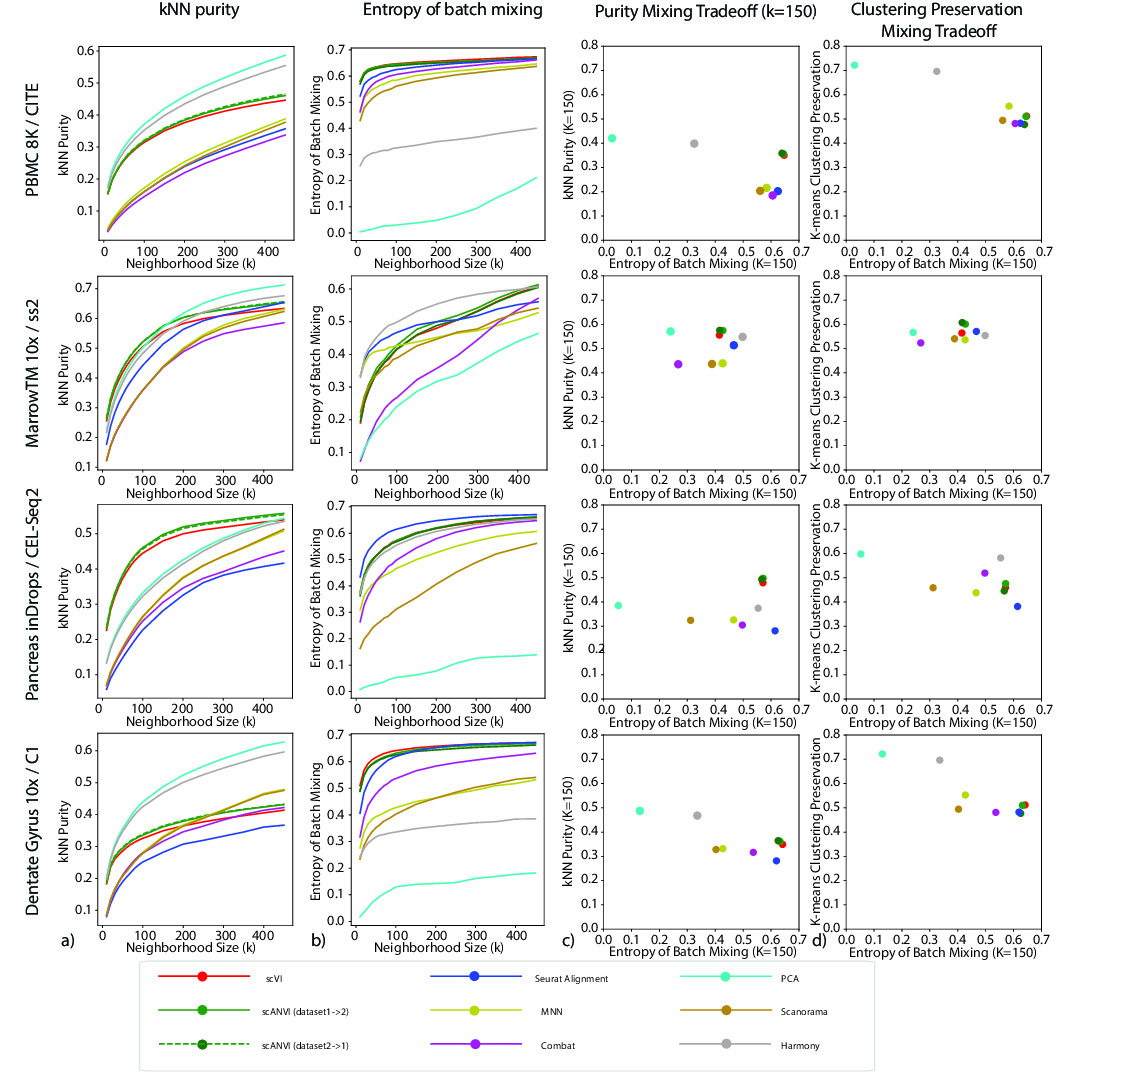
\includegraphics[width=\textwidth]{figures/Fig2.jpeg}
    \caption[Benchmarking of scRNA-seq harmonization algorithms]{Benchmarking of scRNA-seq harmonization algorithms. Each row is a different dataset. Each column is a metric. $(a)$ $k$-nearest neighbors purity that ranges from 0 to 1, with higher values meaning better preservation of neighbor structure in the individual datasets after harmonization. $(b)$ Entropy of batch mixing where higher values means that the cells from different datasets are well-mixed. $(c)$ The trade-off between the $k$NN purity and entropy of batch mixing for a fixed $K=150$. Methods on the top right corner have better performances. $(d)$ The trade-off between entropy of batch mixing and the preservation of biological information using an alternative unsupervised statistic k-means clustering preservation.}
    \label{benchmarking_panel}
    \end{figure}

%%%%%%%%%%%%%%%%%%%%%%%%%%%%%%%%%%%%%%%%%%%%%%%%%%%%%%%%%%%%%%%%%%%%%%%%%
\subsection{Harmonizing datasets with a different composition of cell types}
%%%%%%%%%%%%%%%%%%%%%%%%%%%%%%%%%%%%%%%%%%%%%%%%%%%%%%%%%%%%%%%%%%%%%%%%%
One of the primary challenges of the harmonization problem is handling cases in which the cell types present in the input datasets only partially overlap or do no overlap at all. Since this is a plausible scenario in many applications, it is important to account for it and avoid over-normalizing or ``forcing'' distinct cell populations onto each other. To evaluate this, we performed several stress tests in which we artificially manipulated the composition of cell types in the input datasets prior to harmonization. As our benchmark method we use Seurat Alignment, which performed better than the remaining benchmark methods in our first round of evaluation (Figure~\ref{benchmarking_panel}). 


As a case study, we used a pair of PBMC datasets (PBMC-CITE~\cite{stoeckius2017simultaneous}, PBMC-8K~\cite{10x}) that initially contained a similar composition of immune cell types (Table~\ref{scanvicompo-percent}). We were first interested in the case of no biological overlap~(Figure~\ref{scanvirobustness_panel}a-d). To test this, for a given cell type $c_0$ (e.g., natural killer cells), we only keep cells of this type in the PBMC-CITE dataset and remove all cells of this type from the PBMC-8K dataset. In Figure~\ref{scanvirobustness_panel}a-b, we show an example of UMAP visualization of the harmonized data, with natural killer cells as the left out cell type $c_0$. Evidently, when harmonizing the two perturbed datasets with scVI, the natural killer cells appear as a separate cluster and are not wrongly mixed with cells of different types from the other dataset. Conversely, we see a larger extent of mixing in the latent space inferred by Seurat Alignment. A more formal evaluation is provided in Figure~\ref{scanvirobustness_panel}c-d, which presents our harmonization performance metrics for each cell type averaged across all perturbations (in each perturbation, $c_0$ is set to a different cell type). We also included scANVI with the true number of cell types ($C=6$) in this analysis, using the cell labels from the PBMC-CITE dataset. 

\begin{table}
\centering
\begin{small}
\begin{tabular}{lcc}
    \toprule
 \textbf{cell-type} & \textbf{\begin{tabular}[c]{@{}l@{}}PBMC-8K\\ proportion\end{tabular}} & \textbf{\begin{tabular}[c]{@{}l@{}}PBMC-CITE\\ proportion\end{tabular}}\\[0.2 cm]
 
 \midrule
\textbf{NK cells} & 0.036 & 0.178\\[0.2 cm]

\textbf{CD8 T cells} & 0.119 & 0.091\\[0.2 cm] 

\textbf{B cells} & 0.133 & 0.104\\[0.2 cm]

\textbf{\begin{tabular}[c]{@{}l@{}}FCGR3A+\\ Monocytes\end{tabular}} & 0.028 & 0.029\\[0.2 cm]

\textbf{\begin{tabular}[c]{@{}l@{}}CD14+\\ Monocytes\end{tabular}}  & 0.186 & 0.159\\[0.2 cm]

\textbf{CD4 T} & 0.421 & 0.436\\[0.2 cm]

\textbf{Dendritic Cells} & 0.026 & 0 \\[0.2 cm]

\textbf{Megakaryocytes} & 0.008 & 0 \\[0.2 cm]

\textbf{Other} & 0.043 & 0.004\\
\bottomrule
\end{tabular}
\end{small}
\caption{Composition of cell-types in the PBMC-8K and the PBMC-CITE dataset}
\label{scanvicompo-percent}
\end{table}
 


Under the ideal scenario of a successful harmonization, we expect both a low entropy of batch mixing (since the datasets do not overlap), and retainment of the original structure. Evidently, both scVI and scANVI exhibit a consistently low level of batch mixing that is better or comparable to that of Seurat Alignment, while retaining the original structure more accurately.

As an additional scenario, we investigated the case where the input datasets contain a similar set of cell types, with the exception of one cell type that appears in only one of the datasets. To simulate this, for a given cell type $c_0$, we removed cells of this type from the PBMC-8K dataset, and then harmonize the remaining cells with the unaltered PBMC-CITE (which still contains $c_0$). We show an example of UMAP visualization in Figure~\ref{scanvirobustness_panel}e-f, removing CD4+ T cells from the PBMC-8K dataset. Evidently, in the scVI latent space, the PBMC-CITE ``unique'' CD4+ T cell population is not wrongly mixed with cells from the perturbed PBMC-8K dataset, but rather appears as a distinct cluster. For a more formal analysis, Figure~\ref{scanvirobustness_panel}g-i shows the harmonization statistics for perturbing the six major cell types present in the PBMC datasets. As above, we also evaluated scANVI in this context, using the labels from the unperturbed (PBMC-CITE) dataset.


Figure~\ref{scanvirobustness_panel}g shows that the entropy of batch mixing from the ``unique'' population (averaging over all six perturbations) is low in all three methods (scVI, scANVI and Seurat Alignment), with a slight advantage for scVI and scANVI. Figure~\ref{scanvirobustness_panel}h-i shows the harmonization statistics for each population, averaging over all shared cell types between the two datasets. Evidently, for the populations that are indeed common to the two datasets, scVI and scANVI are capable of mixing them properly, while preserving the original structure, comparing favorably to Seurat Alignment on both measures. Overall, the results of this analysis demonstrate that scVI and scANVI are capable of harmonizing datasets with very different compositions, while not forcing erroneous mixing. These results are consistent with the design of scVI and scANVI, which aim to maximize the likelihood of a joint generative model, without making \textit{a priori} assumptions about the similarity in the composition of the input datasets.

In a similar but more complex experiment, we also study the case when the two datasets both have their own unique cell types but also share several common cell types. Populations unique to each dataset have low mixing (Figure~\ref{scanviunique_pops}a), especially with scVI and scANVI. Conversely, the shared populations have a substantially higher mixing rate (Figure~\ref{scanviunique_pops}c). Specifically, scANVI and scVI both mix shared populations better than Seurat, with a better overall performance for scANVI. Finally, the preservation of original structure is higher scVI and scANVI when compared to Seurat across all cell types, especially for B cells, NK cells and FCGR3A+ Monocytes (Figure~\ref{scanviunique_pops}b). Overall, these results demonstrate that our methods do not tend to force wrong alignment of non-overlapping parts of the input datasets.


\begin{figure}[htp]
\centering
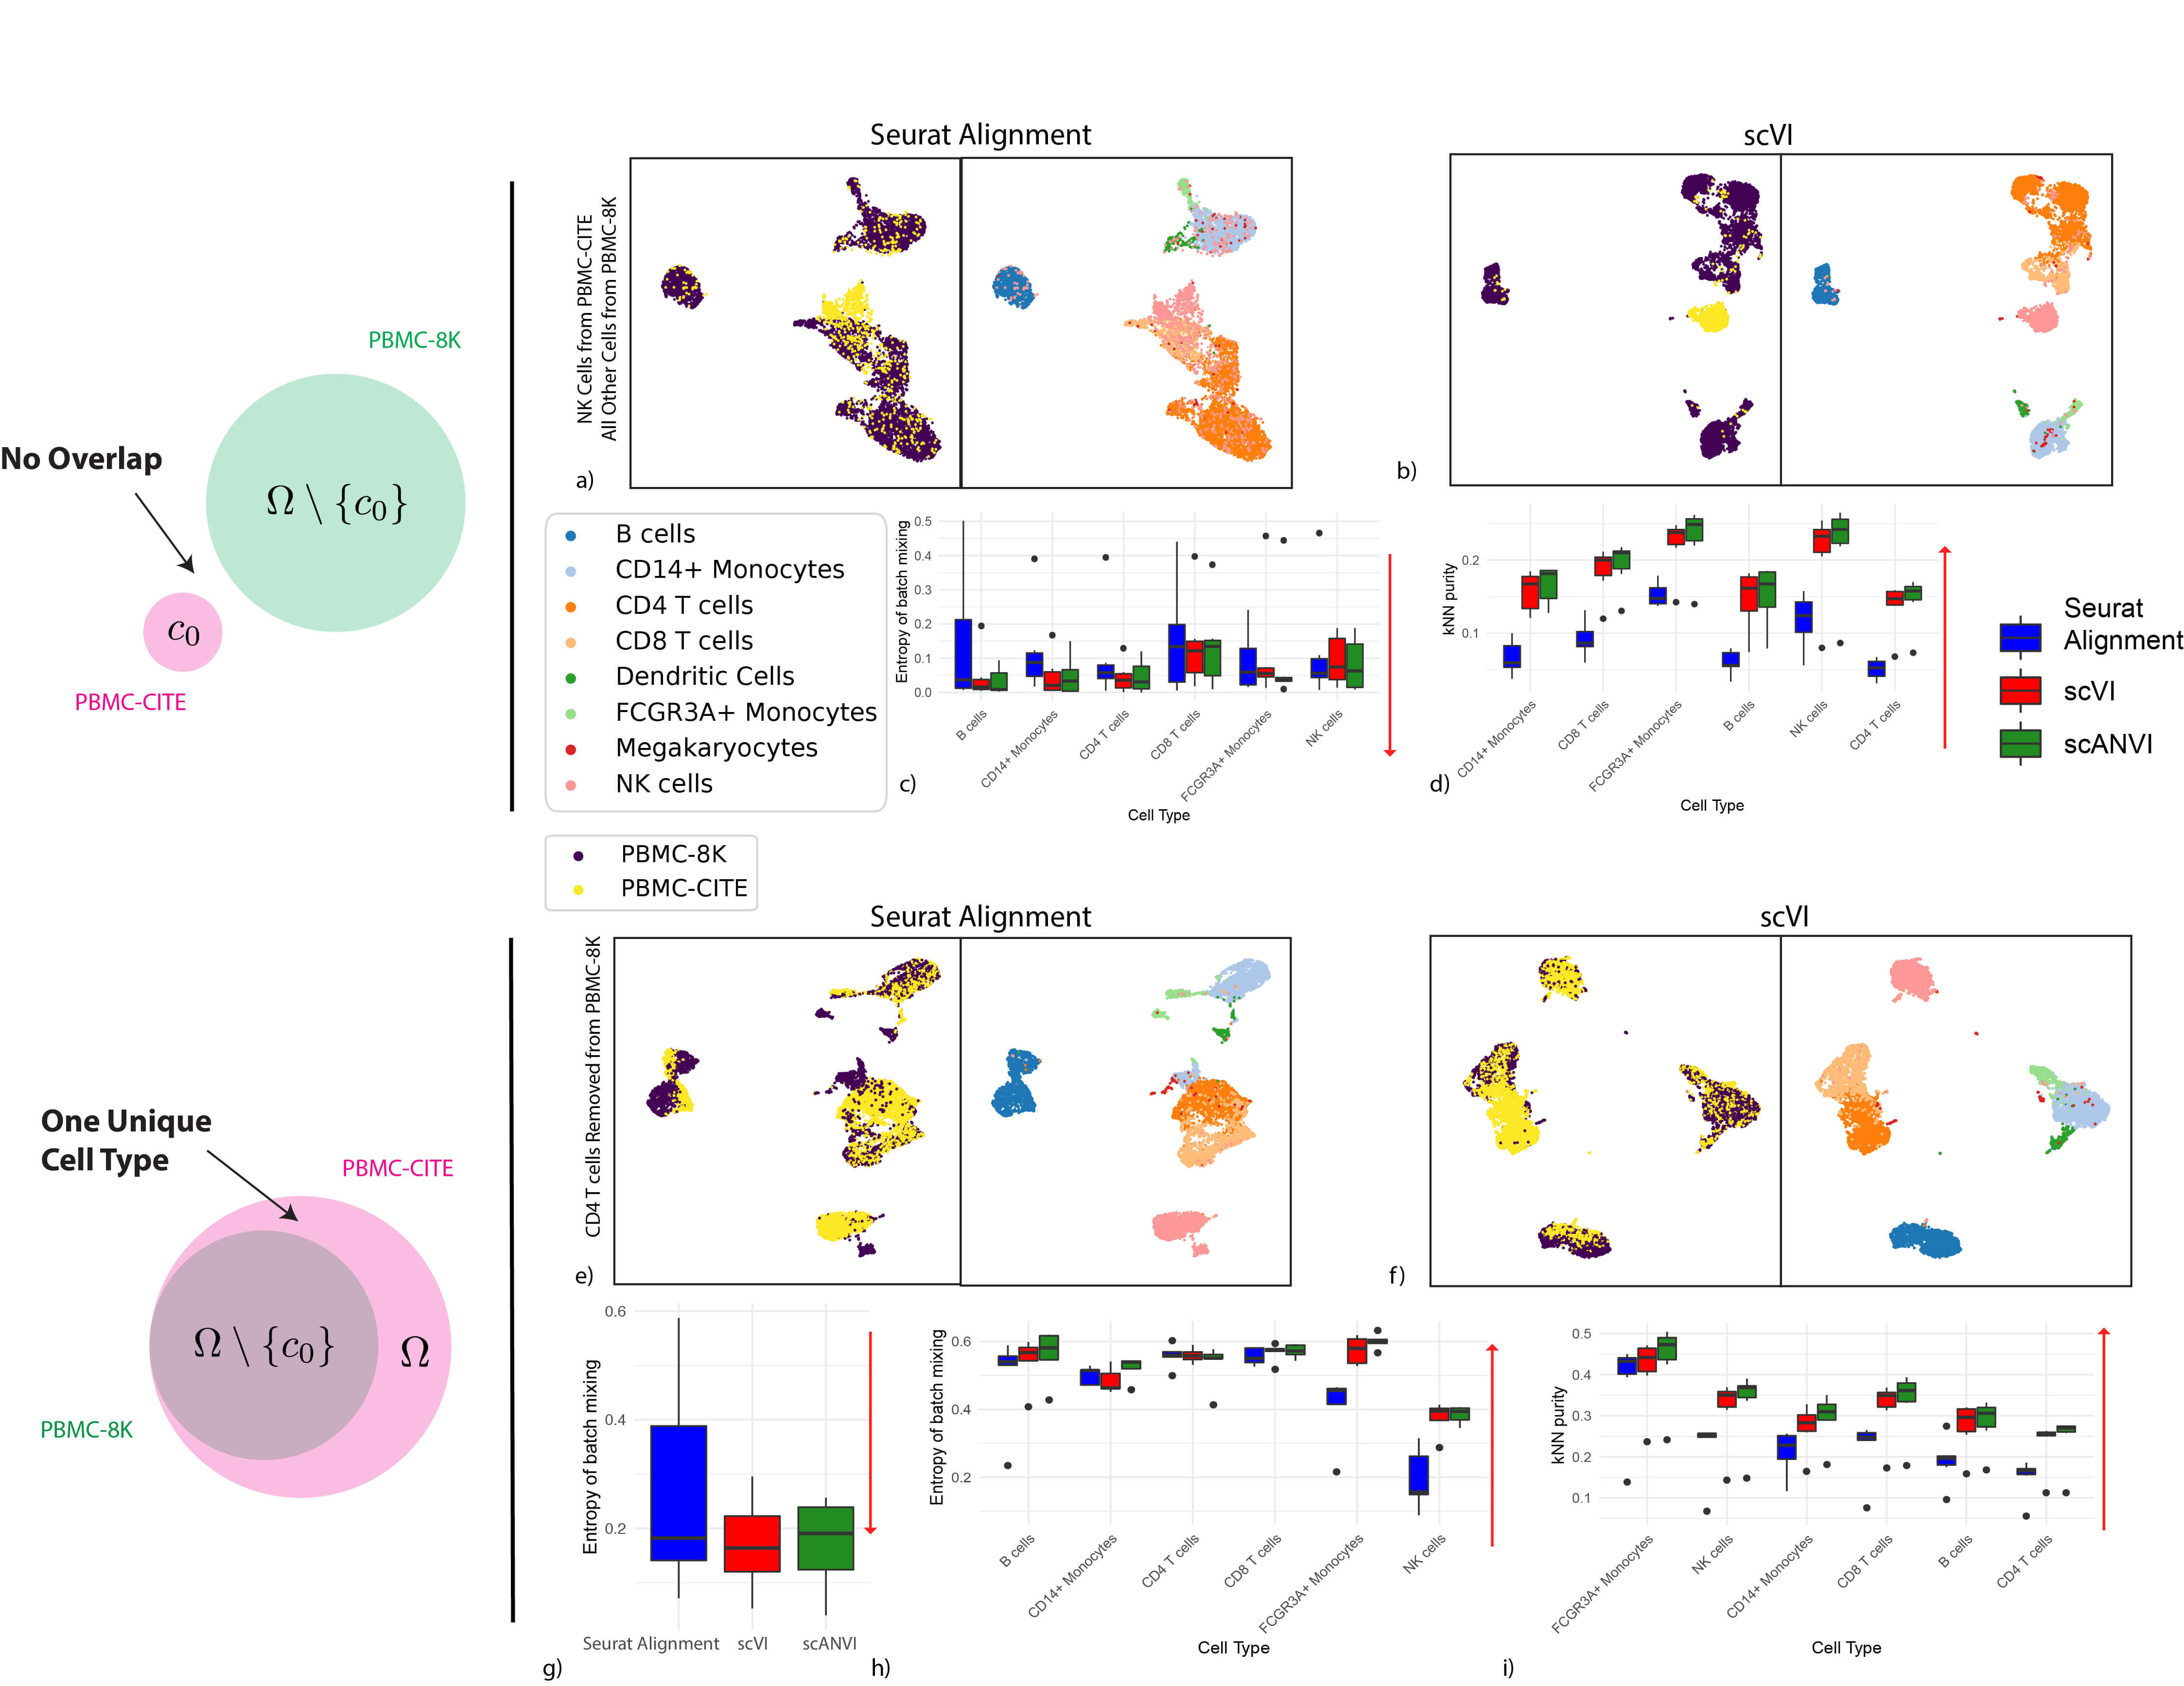
\includegraphics[width=\textwidth]{figures/Fig3.jpg}
\caption[Harmonizing datasets with different cellular composition]{Harmonizing datasets with different cellular composition. $(a-d)$ show the case when no cell type is shared. PBMC-8K contains all cells other than cell type $c_0$ while PBMC-CITE contains only cell type $c_0$. $(a-b)$ UMAP visualization for the case where $c_0$ corresponds to natural killer cells. $(c-d)$ entropy of batch mixing and $k$-nearest neighbors purity, aggregating the six experiments (setting $c_0$ to a different cell type in each experiment). $(e-i)$ show the case when cell type $c_0$ is removed PBMC-8K but not from PBMC-CITE. $(e-f)$ UMAP visualization for the case where $c_0$ corresponds to CD4+ T cells. $(g)$ entropy of batch mixing for the removed cell type. $(h)$ entropy of batch mixing for the remaining cell types. $(i)$ $k$-nearest neighbors purity, aggregating all 6 experiments. Red arrows indicate the desired direction for each performance measure (e.g., low batch entropy is desirable in $(d)$). The boxplots are standard Tukey boxplots where the box is delineated by the first and third quartile and the whisker lines are the first and third quartile plus minus 1.5 times the box height. The dots are outliers that fall above or below the whisker lines.}
\label{scanvirobustness_panel}
\end{figure}


%%%%%%%%%%%%%%%%%%%%%%%%%%%%%%%%%%%%%%%%%%%%%
\subsection{Harmonizing continuous trajectories}
%%%%%%%%%%%%%%%%%%%%%%%%%%%%%%%%%%%%%%%%%%%%%%%%%%%%%%
While so far we considered datasets that have a clear stratification of cells into discrete sub-populations, a conceptually more challenging case is harmonizing datasets in which the major source of variation forms a continuum, which inherently calls for accuracy at a higher level of resolution. 

To explore this, we use a pair of datasets that provides a snapshot of hematopoiesis in mice (HEMATO-Tusi \cite{Tusi2018}, HEMATO-Paul \cite{PAUL2015}; Figure~\ref{scanvicontinuous_panel}). These datasets consist of cells along the transition from common myeloid progenitor cells (Figure~\ref{scanvicontinuous_panel}a-b; middle) through two primary differentiation trajectories myeloblast (top) and erythroblast-megakaryocyte (bottom). Notably, the HEMATO-Tusi dataset contains cells that appear to be more terminally differentiated, which are located at the extremes of the two primary branches. This can be discerned by the expression of marker genes (Figure~\ref{scanvicontinuous_panel}e). For instance the HEMATO-Tusi unique erythroid cell population expresses \textit{Hba-a2} (hemoglobin subunit) and \textit{Alas2} (erythroid-specific mitochondrial 5-aminolevulinate synthase) that are known to be present in reticulocytes \cite{Ery2007,MTAB}. At the other end, the granulocyte subset that is captured only by HEMATO-Tusi expresses \textit{Itgam} and \textit{S100a8}. \textit{S100a8} is a neutrophil specific gene predicted by Nano-dissection \cite{nano2013} and is associated with GO processes such as leukocyte migration associated with inflammation and neutrophil aggregation. \textit{Itgam} is not expressed in granulocyte-monocyte progenitor cells but is highly expressed in mature monocytes, mature eosinophils and macrophages~\cite{papatheodorou2017expression}. We therefore do not expect mixing to take place along the entire trajectory. To account for this, we evaluated the extent of batch entropy mixing at different points along the harmonized developmental trajectory. As expected, we find that in most areas of the trajectory the two datasets are well mixed, while at the extremes, the entropy reduces significantly, using either scVI or Seurat Alignment (Figure~\ref{scanvicontinuous_panel}c). Overall, we observe that scVI compares well in terms of both mixing the differentiation trajectories in each dataset and preserving their original, continuous, structure (Figure~\ref{scanvicontinuous_panel}a-d). 

To validate scANVI in this context as well, we provided it with the categorical labels of cells along the two developmental trajectories, indicating their cell state (Figure~\ref{scanvicontinuous_panel}c-d and Figure~\ref{scanvicontinuousSupp}). Even though this labeling scheme does not explicitly account for the ordering between states, we observe that scANVI is capable of mixing the two datasets, while retaining their original structure, achieving a level of accuracy comparable to that of scVI and better than that of Seurat Alignment. 


\begin{figure}[htp]
\centering
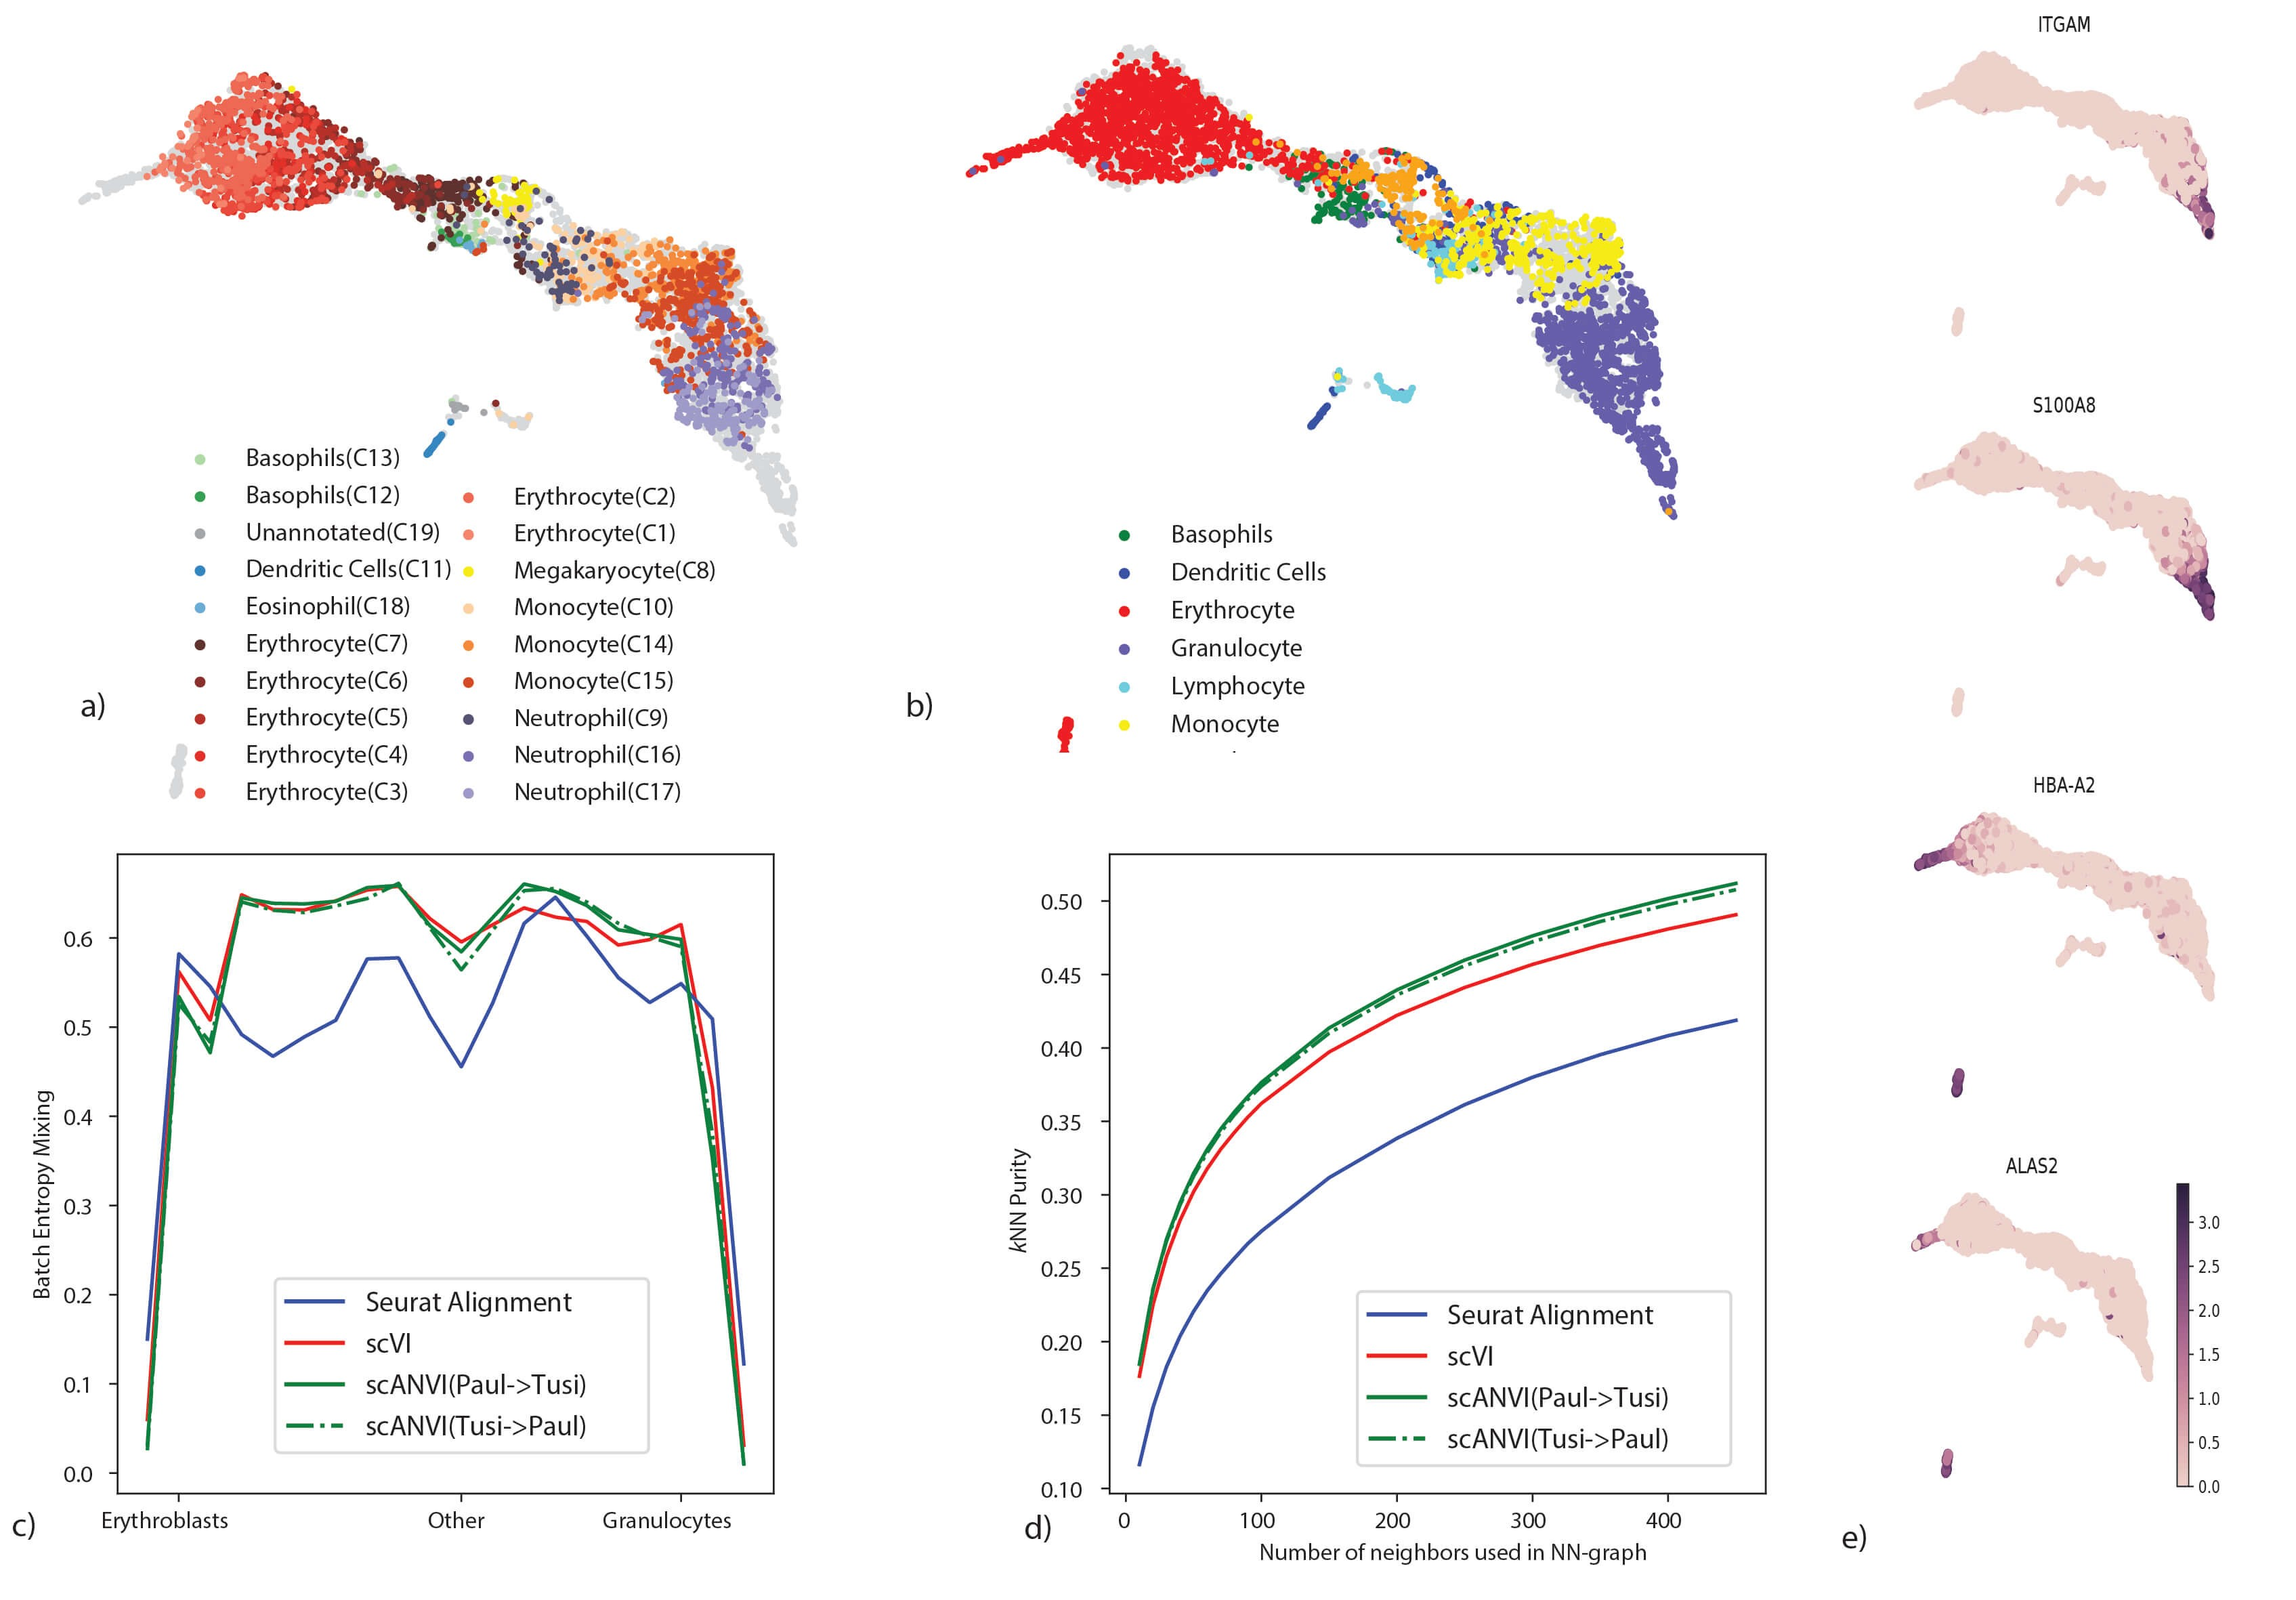
\includegraphics[width=\textwidth]{figures/continuous.jpg}
\caption[Harmonizing developmental trajectories]{Harmonizing developmental trajectories. $(a-b)$ UMAP visualization of the scVI latent space, with cells colored by the original labels from either the HEMATO-Paul $(a)$ or HEMATO-Tusi $(b)$ studies. The cells from the other dataset are colored in gray. $(c)$ Entropy of batch mixing along 20 bins of the HEMATO-Tusi cells, ordered by the potential of each cell. Potential is a pseudotime measure that describes the differentiation state of a cell using the population balance analysis algorithm (center: common myeloid progenitors; moving left: erythrocyte branch; moving right: granulocyte branch). $(d)$ $k$-nearest neighbors purity for scVI, Seurat, and scANVI. $(e)$ Expression of marker genes that help determine the identity of batch-unique cells.} 
\label{scanvicontinuous_panel}
\end{figure}

%%%%%%%%%%%%%%%%%%%%%%%%%%%%%%%%%%%%%%%%%%%%%%%%%%%%%%
\subsection{Rapid integration of multiple datasets}
%%%%%%%%%%%%%%%%%%%%%%%%%%%%%%%%%%%%%%%%%%%%%%%%%%%%%%

To demonstrate the scalability of our framework in the context of harmonizing multiple (and possibly large) dataset, we ran scVI to integrate a cohort of 26 datasets spanning 105,476 cells from multiple tissues and technologies, which was made available by the authors of Scanorama (a method based on truncated singular value decomposition followed by nearest neighbor matching ~\cite{scanorama}). Using the hardware specified in the original paper~\cite{scanorama} (Intel Xeon E5-2650v3 CPU limited to 10 cores with 384 GB of RAM), Seurat Alignment and MNN required over 24 hours, while Scanorama completed its run in 20 minutes. Using a simpler configuration (eight-core Intel i7-6820HQ CPU with 32 GB RAM) along with one NVIDIA Tesla K80 GPU (GK210GL; addressing 24 GB RAM), we found that scVI integrates all datasets and learns a common embedding in less than 50 minutes. This running time is competitive considering the reduced memory availability and the increased complexity of our model, compared to that of Scanorama. Notably, all the downstream analyses, such as annotation, differential expression or visualization can be operated by accessing the latent space or via forward passes through the neural networks. Since these access operations can be conducted very efficiently~\cite{scvi}, the dominant factor, on which we focused our run time analysis, is the time required for model fitting. Considering the results, the latent space of scVI recapitulates well the major tissues and cell types~(Figure~\ref{scanvilarge_scale_panel}), and the position of cells in the latent space provides an effective predictor for the cell type label (Figure~\ref{scanvilarge_scale_panel}).


%%%%%%%%%%%%%%%%%%%%%%%%%%%%%%%%%%%%%%%%%%%%%%%%%%%%%%
\subsection{Transferring cell type annotations between datasets}
%%%%%%%%%%%%%%%%%%%%%%%%%%%%%%%%%%%%%%%%%%%%%%%%%%%%%%

We next turned to evaluate scVI and scANVI in the context of harmonization-based annotation. Here, we test the extent to which annotations from a previously annotated dataset can be used to automatically derive annotations in a new unannotated dataset. For scVI and Seurat Alignment, we derive the annotations by first harmonizing the input datasets and then running a $k$-nearest neighbors classifier (setting $k$ to 10) on the joint latent space, using the annotated cells to assign labels to the unannotated ones. Conversely, scANVI harmonizes the input datasets while using any amount of available labels. The prediction of unobserved labels is then conducted using the approximate posterior assignments $q_\Phi(c \mid x)$ of cell types, directly derived from the model. An alternative approach that we benchmark against was taken by scmap-cluster~\cite{scmap}. scmap directly builds a classifier based on the labeled cells (instead of performing harmonization first) and then applies this classifier to the unlabeled cells. Finally, we also applied the domain adaptation method Correlation Alignment for Unsupervised Domain Adaptation (CORAL,~\cite{sun2016return}). This method was not initially developed for single-cell analysis but is an insightful benchmark from the machine learning literature.

We start by exploring the four dataset pairs in Figure~\ref{benchmarking_panel}, which have been annotated in their respective studies. In each experiment, we ``hide'' the cell type annotations from one dataset and transfer the second dataset labels to the first one. As a measure of performance, we report the weighted accuracy, which is the percent of cells that were correctly assigned to their correct (hidden) label, averaging over all labels. Importantly, the annotations in this first set of case studies were derived computationally. For example, by first clustering the cells, looking for marker genes expressed by each cluster and then assigning labels to the clusters accordingly. This level of annotation therefore makes the prediction problem relatively easy, and indeed, while we find that overall scANVI predicts unobserved labels more accurately, the differences between the methods are mild (Figures~\ref{scanviaccbox} and~\ref{scanvibubble}). Notably, CORAL achieves overall competitive performance except when transferring labels on the MarrowTM pairs, from 10x to Smart-Seq2. In this specific instance, CORAL maps most of the cells to a single label (incidentally, while this label marks cells that are transcriptionally similar, it is defined by the authors as an unknown class ``NA'', corresponding to cells that cannot be confidently assigned or low quality cells according to the authors of \cite{quake2018single}), which might be due to its linear transformation of the feature space. 


To evaluate the accuracy of annotations without the need for computationally-derived labels, we turned to the PBMC-CITE dataset which includes measurements of ten key marker proteins in addition to mRNA~\cite{stoeckius2017simultaneous}, and the PBMC-sorted dataset~\cite{zheng2017massively}, where cells were collected from bead purifications for eleven cell types (Table~\ref{scanvipbmc-pure-celltypes}). We applied scVI and scANVI to harmonize and annotate these two datasets along with a third dataset of PBMC (PBMC-68K~\cite{zheng2017massively}). Our analysis contains a combined set of $n=169,850$ cells from the three datasets altogether. To generate a realistic scenario of cell type annotation, we only provide access to the experimentally-based labels from the PBMC-sorted dataset (Figure~\ref{scanviconcordance_panel}a-c). As an additional benchmark, we also evaluate Seurat Alignment, which was tested after removal of a randomly selected subset ($40 \%$) of the two large datasets (PBMC-68K and PBMC-sorted) due to scalability issues. Considering our harmonization performance measures (i.e., retainment of the original structure and batch mixing), we observe as before that scVI and scANVI perform similarly and compare favorably to Seurat Alignment. We then evaluated the accuracy of assigning unobserved labels, focusing on the PBMC-CITE dataset. Instead of using the labels from the original PBMC-CITE study as ground truth (which were computationally derived), we used the protein data, which provides an experimentally-derived proxy for cell state. To this end, we quantified the extent to which the similarity between cells in the harmonized mRNA-based latent space is consistent with their similarity at the protein level. We first computed the average discrepancy (sum of squared differences) between the protein measurements in each cell and the average over its $k$-nearest neighbors. As a second measure we computed for each PBMC-CITE cell the overlap between its $k$-nearest PBMC-CITE neighbors in the harmonized mRNA-based space and in the protein space. We then report the average across all cells in Figure~\ref{scanviconcord_supplement}. Evidently, scANVI outperformed both scVI and Seurat Alignment for a wide range of neighborhood sizes, providing a representation for the mRNA data that is more consistent with the protein data (Figure~\ref{scanviconcordance_panel}c).


\begin{table}
\centering
\begin{small}
\begin{tabular}{lc}
    \toprule
\textbf{Cell Types}        & \textbf{\# cells} \\
\midrule
\textbf{B cells}           & 10,085   \\
\textbf{CD14+ Monocytes}   & 2,612    \\
\textbf{CD34+ cells}       & 9,232    \\
\textbf{CD4 T cells}       & 11,213   \\
\textbf{CD56 NK cells}     & 8,385    \\
\textbf{CD8 T cells}       & 10,209   \\
\textbf{Memory T cells}   & 10,224   \\
\textbf{Naive CD8 T cells} & 11,953   \\
\textbf{Naive T cells}     & 10,479   \\
\textbf{Regulatory T cells}     & 10,263   \\
\bottomrule
\end{tabular}
\end{small}
\caption{Cell types present in the PBMC-sorted dataset.}
\label{scanvipbmc-pure-celltypes}
\end{table}
 

\begin{figure}
\centering
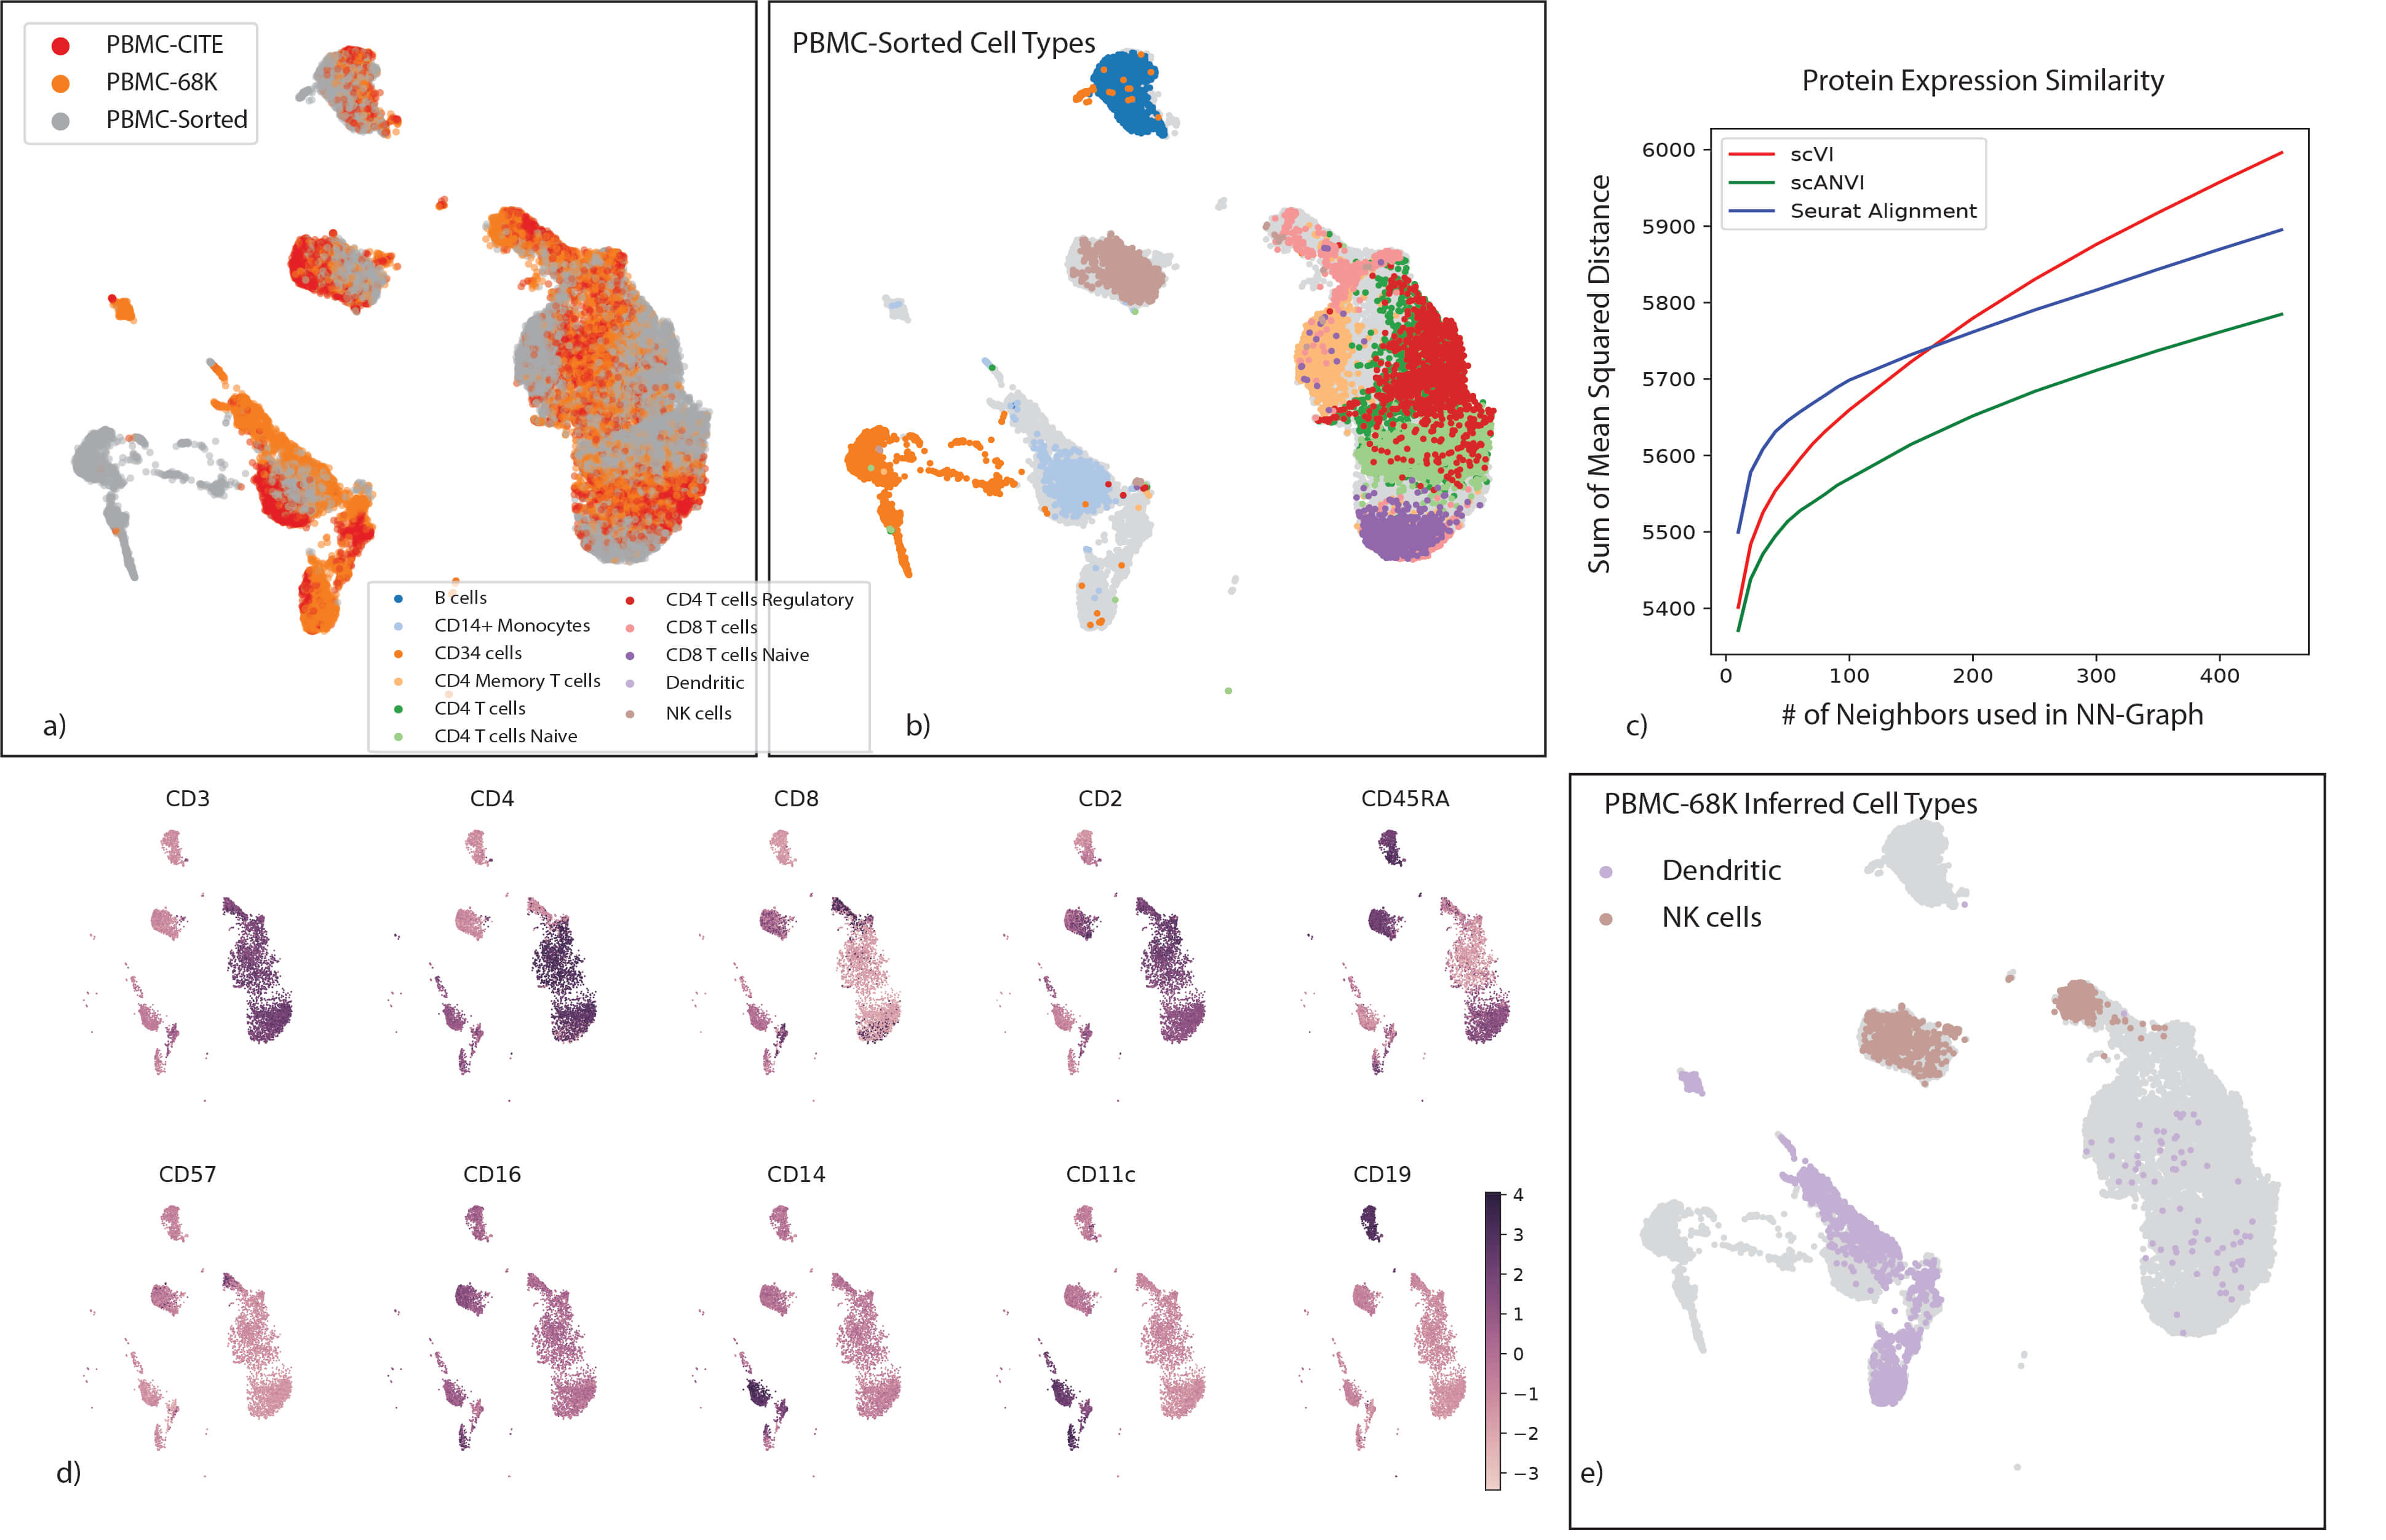
\includegraphics[width=\textwidth]{figures/labels_concored.jpg}
\caption[Validation of cell type annotations using additional metadata]{Validation of cell type annotations using additional metadata. (a-b) UMAP plot of the scANVI latent space inferred for three harmonized datasets: PBMC-CITE, PBMC-sorted, and PBMC-68K. Cells are colored by the dataset of origin $(a)$ and the PBMC-sorted labels $(b)$. Cells from the PBMC-CITE and PBMC-68K are colored in gray in $(b)$. (c) The consistency of the harmonized PBMC-CITE mRNA data with the respective protein measurements, evaluated by mean squared error and for different neighborhood size. Lower values indicate higher consistency. $(d)$ UMAP plot of the scANVI latent space, where cells are colored by normalized protein measurement. Only PBMC-CITE cells are displayed. $(e)$ UMAP plot of the scANVI latent space, with cells from the PBMC-68k dataset colored according to their original label. For clarity of presentation, only cells originally labeled as dendritic cells or natural killer cells are colored. Evidently, a large number of these cells are mapped to a cluster of T-cells (right side of the plot).}
\label{scanviconcordance_panel}
\end{figure}


%%%%%%%%%%%%%%%%%%%%%%%%%%%%%%%%%%%%%%%%%%%%%%%%%%%%%%
\subsection{Cell type annotation in a single dataset based on ``seed'' labels}
%%%%%%%%%%%%%%%%%%%%%%%%%%%%%%%%%%%%%%%%%%%%%%%%%%%%%%
An important variant of the annotation problem lies within the context of an \textit{ab initio} labeling of a single dataset where only a subset of the cells can be confidently annotated based on the raw data. This increasingly prevalent scenario may result from limited sensitivity of the scRNA-seq assay, where marker genes may only be confidently observed in a small subset of cells. One common way to address this problem is to compute some form of a distance metric between cells (e.g., after embedding with scVI or using Seurat PCA) and then assign labels based on proximity to annotated cells \cite{zheng2017massively}. To benchmark our methods, we consider two such predictors: the first is clustering the cells and taking a majority vote inside each cluster, and the second is taking the majority vote of the $k$-nearest neighbors around each unannotated cell ($k=10$). While these approaches are quite straightforward, their accuracy might suffer when the data do not form clear clusters~\cite{Tusi2018}, or when differences between labels are too subtle to be captured clearly by a transcriptome-wide similarity measure. To address these issues, scANVI takes an alternative approach, namely learning a latent embedding that is guided by the available labels, and then producing posterior probabilities for assigning labels to each cell. 

As a case study, we compiled a dataset consisting of several experimentally sorted and labeled subsets of T cells from the PBMC-sorted dataset, including CD4 memory, CD4 naive, CD4 regulatory and CD8 naive. To make our analysis more realistic, we assume that the labels are completely unknown to us and therefore assign each T cell to its respective subset using marker genes (12 altogether):
\begin{itemize}
    \item \textbf{CD4 regulatory}: \textit{GITR}$^+$ \textit{CTLA4}$^+$ \textit{FOXP3}$^+$ \textit{CD25}$^+$ \textit{S100A4}$^-$\textit{CD45}$^-$\textit{CD8B}$^-$
    \item \textbf{CD4 naive}: \textit{CCR7}$^+$ \textit{CD4}$^+$ \textit{S100A4}$^-$\textit{CD45}$^-$\textit{FOXP3}$^-$\textit{IL2RA}$^-$\textit{CD69}$^-$
    \item \textbf{CD4 memory}: \textit{S100A4}$^+$ \textit{CD25}$^-$\textit{FOXP3}$^-$\textit{GITR}$^-$\textit{CCR7}$^-$
    \item \textbf{CD8 naive}: \textit{CD8B}$^+$ \textit{CCR7}$^+$ \textit{CD4}$^-$
    \end{itemize}
Notably, several important biomarkers (\textit{CD4}, \textit{CTLA4}, and \textit{GITR}) are detected in less than $5 \%$ of the cells. This renders their use for annotation not straightforward. Furthermore, many of these biomarkers are sparsely expressed to the extent that they are likely to be filtered out in the gene selection step of most harmonization procedures (Figure~\ref{scanviscanvi_panel}a). 


To analyze this dataset, we first computed a signature score for each cell and for each label (i.e., T cell subset) using the scaled raw expression values of the respective marker genes. We then designated the top $50$ scoring cells in each subset as the seed set of cells that are confidently annotated for that subset (Figure~\ref{scanviscanvi_panel}b). Reassuringly, this partial annotation is in agreement with the experimentally-derived cell type labels available for this dataset (Figure~\ref{scanviscanvi_panel}c). However, this dataset does not form clear clusters, and in particular the seed sets of cells are not well separated. Such an observation makes clustering-based approaches potentially less precise. Indeed, using $k$-means clustering on the scVI and Seurat PCA latent space, we find that $74 \%$ and $72\%$ of the cells were assigned with their correct label. Similar analysis with two additional popular clustering algorithms (DBSCAN~\cite{dbscan} and PhenoGraph~\cite{Levine_PhenoGraph_2015}) further emphasizes the challenge of a cluster-based approach on this data. Specifically, DBSCAN does not partition the data into more than one cluster (scanning through a large number of parameter values), and PhenoGraph predicts 9 clusters and achieves an accuracy of $41 \%$ (Figure~\ref{scanviscanviClustering}). 

%Chenling: Fig 6: panel B needs to scVI

Consistent with these results, the application of a $k$-nearest neighbors classifier resulted in a similar level of accuracy in the Seurat PCA latent space ($71 \%$), which is slightly improved when replacing it with the scVI latent space ($73 \%$; Figure~\ref{scanviscanviClustering}). Conversely, after fitting the scANVI model based on this partial labeling, the annotation posterior $q_\Phi(c \mid z)$ (Figure~\ref{scanviscanvi_panel}d) provides a substantially more accurate cell type assignment, with $84 \%$ of cells annotated correctly. 

While scANVI has been designed to handle discrete (but not continuous) labels, we hypothesized that gradual transition between cell states may still be captured by the uncertainty of label assignment. We tested it using simulated data~\cite{symsim} that consists of a set of ``end-point'' states along with intermediary states that connect them (Figure~\ref{scanvisymsim_cont}a). We provided labels only to end-point cells, and investigated the label assignment scores calculated for the intermediary cells. We find that scANVI provides a range of assignment probability values and that these values are proportional to the distance from the respective end points (Figure~\ref{scanvisymsim_cont}b-g). Conversely, the scores provided by scmap tend to be more extreme (Figure~\ref{scanvisymsim_cont}h-i), thus less reflecting the continuous nature of the data.



\begin{figure}[ht]
\centering
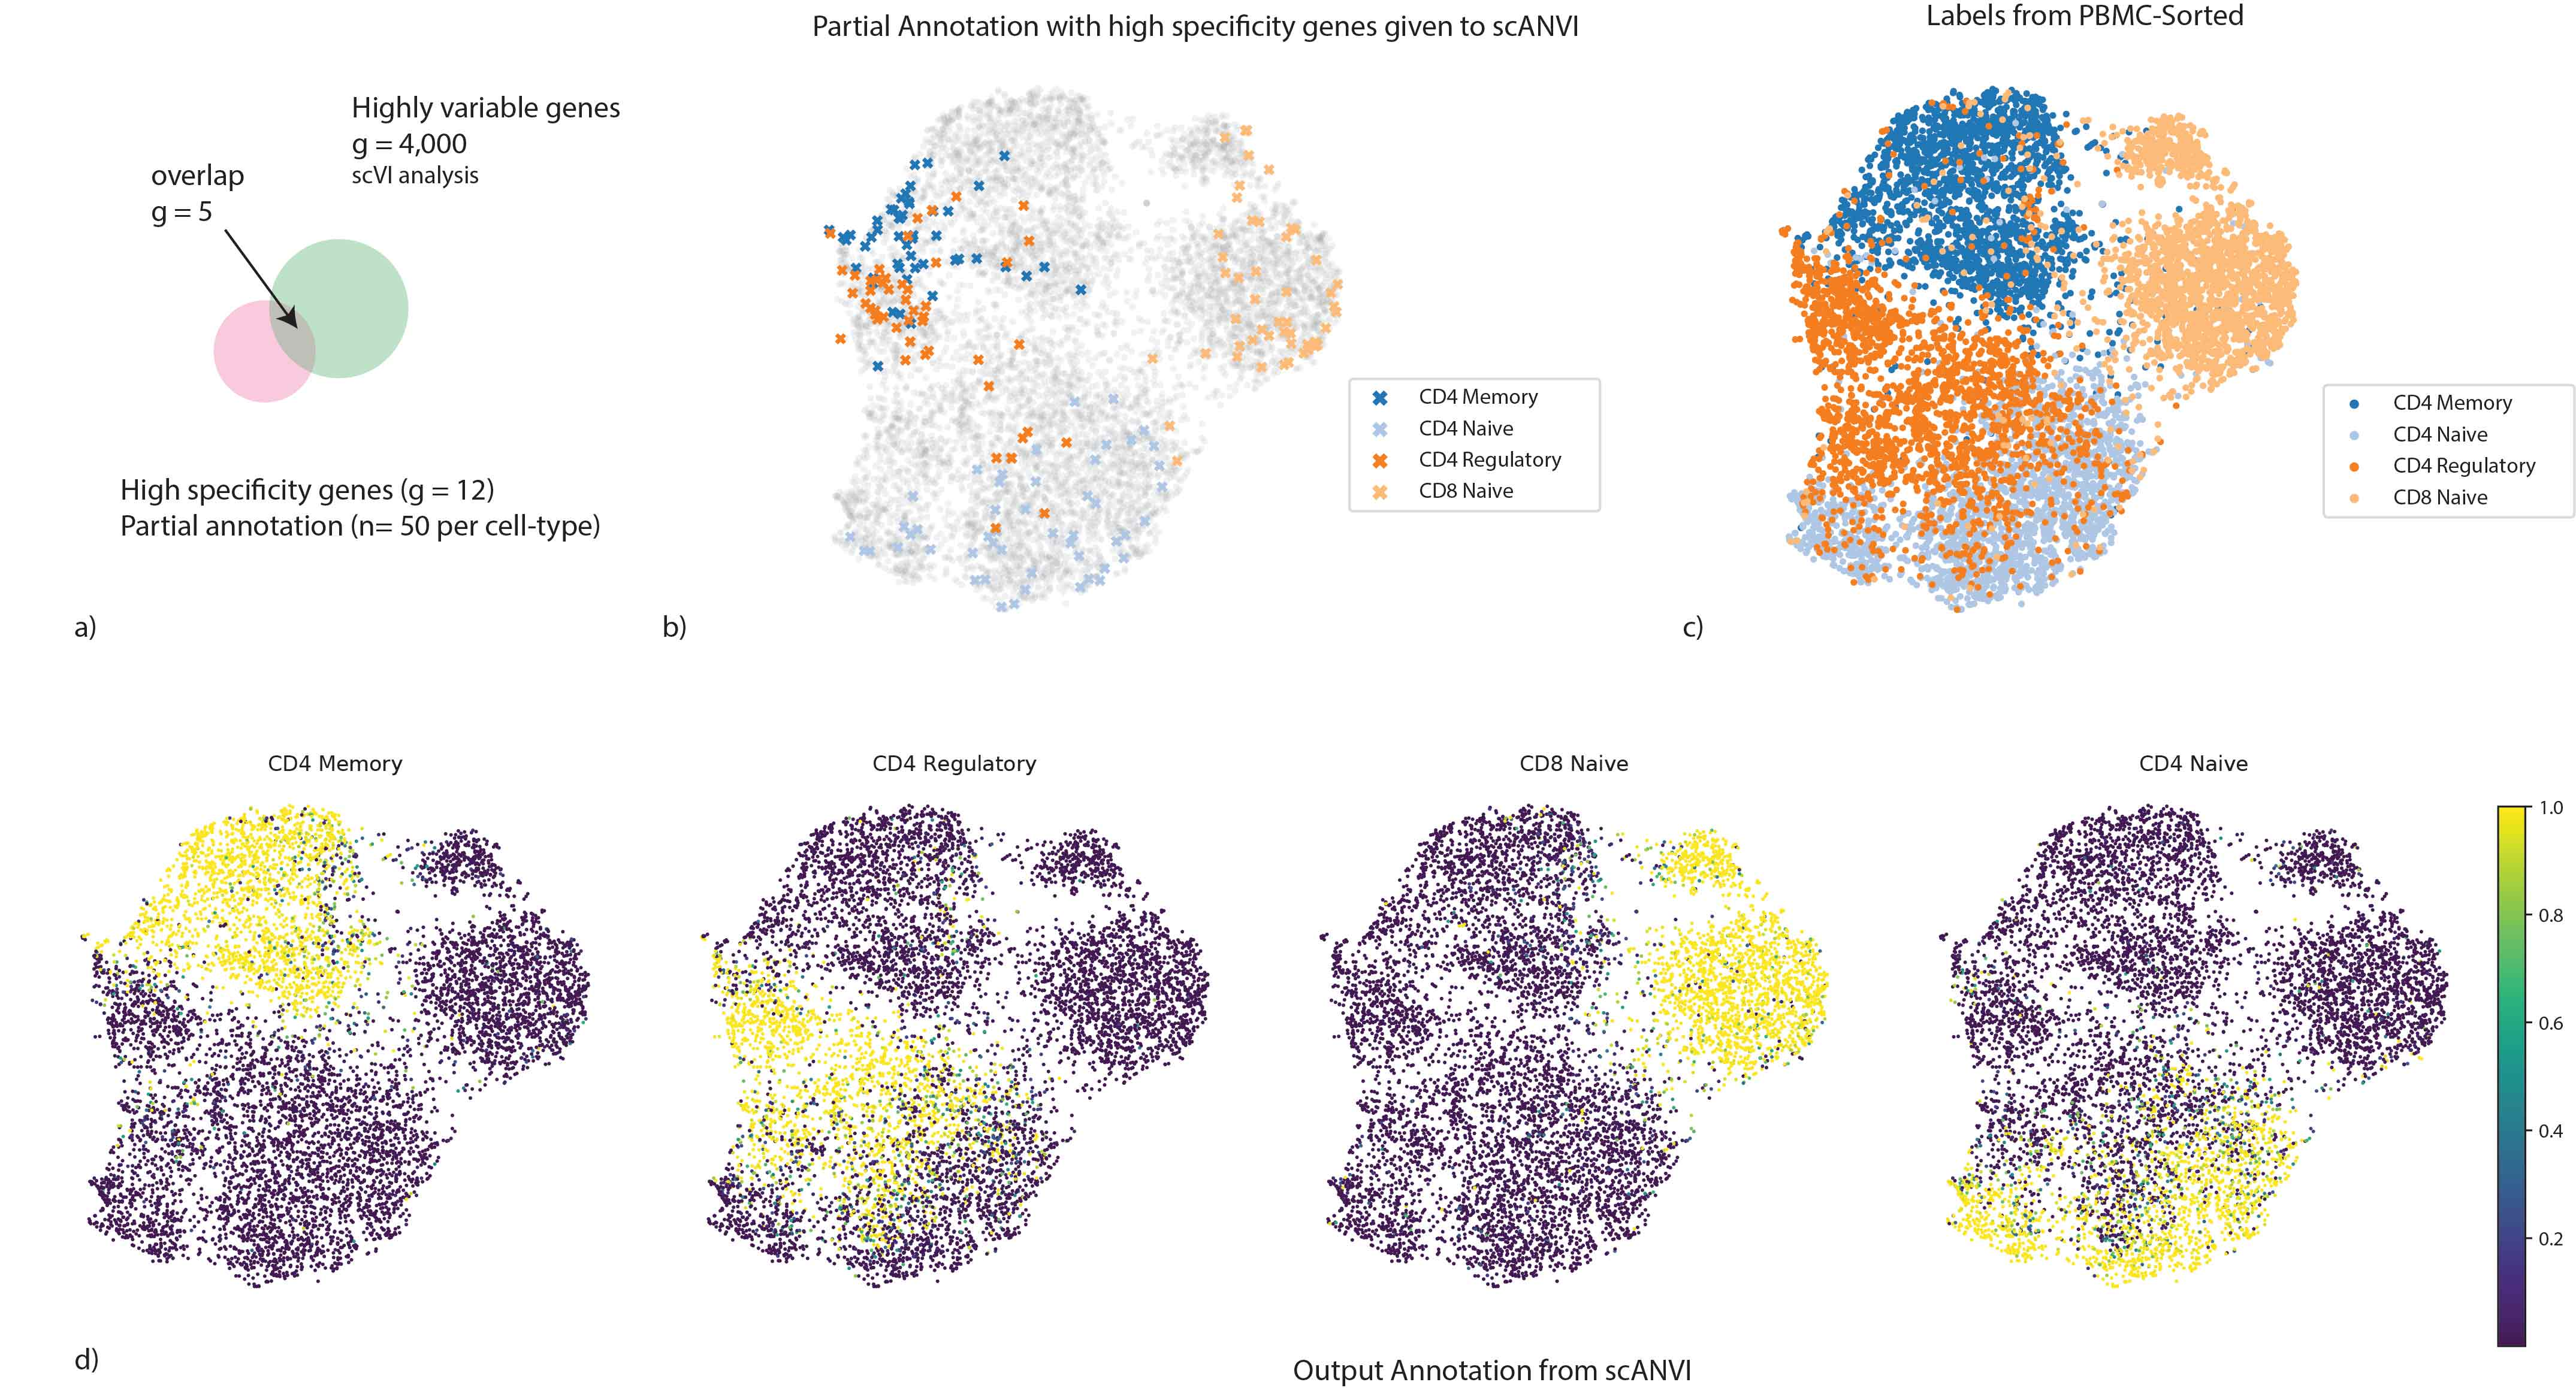
\includegraphics[width=\textwidth]{figures/scanvi.jpg}
\caption[Cell type annotation in a single dataset using ``seed'' labeling]{Cell type annotation in a single dataset using ``seed'' labeling. $(a)$ discrepancies between marker genes that can be used to confidently label cells and highly variable genes in scRNA-seq analysis. $(b-d)$ UMAP plot of the scVI latent space. $(b)$ Seed cells are colored by their annotation (using known marker genes). $(c)$ PBMC-sorted cell type labels from the original study based on marker-based sorting $(d)$ The posterior probability of each cell being one of the four T cell subtypes obtained with scANVI.}
\label{scanviscanvi_panel}
\end{figure}


%%%%%%%%%%%%%%%%%%%%%%%%%%%%%%%%%%%%%%%%%%%%%%%%%%%%%%
\subsection{Cell type taxonomy and hierarchical classification with scANVI}
%%%%%%%%%%%%%%%%%%%%%%%%%%%%%%%%%%%%%%%%%%%%%%%%%%%%%%
Another subtle yet important variation of the annotation problem is when the labels are not mutually exclusive but rather form a taxonomy of cell types or states. To effectively annotate cells in this setting, we extended scANVI to perform hierarchical classification, which as before we carry out from first principles, relying on probabilistic graphical models. 

\subsubsection{Hierarchical classification of cells onto a cell type taxonomy}
For hierarchical label propagation in scANVI, we propose a extension of the formerly presented model by modifying the variable $c_n$ to be a tuple where each entry denotes the label at a given level of the hierarchy. Our approach is similar to previous work in robustness to noisy labels~\cite{goldberger2016training} and hierarchical multi-labels flavors of classification problems~\cite{pmlr-v80-wehrmann18a}. We now detail the case for a depth of level two in though our approach can in principle be adapted to arbitrary depths. In our setting, the taxonomy needs to be hard-coded and known \textit{a priori}.

We do not modify the generative model but only the structure of the variable~$c_n$ in the variational distribution. Notably, we formally pose: 
\begin{align}
    c_n = (y_n, y^g_n) \in \{0, \ldots, C\} \times \{0, \ldots, C^g\},
\end{align} 
where $C$ denotes the number of cell types and $C^g$ the number of cell type groups. The parametrization of the full variational distribution $q(c \mid z) = q(y, y^g \mid z)$ must be further defined. For this, we notice that the prior taxonomy knowledge encapsulates whether the assignment $(y^g, y) = (i, j)$ is biologically possible (i.e cell type $i$ is a sub-population of group cell type $j$). We encode this biological compatibility into a parent function $\pi: \{0, \ldots, K\} \rightarrow \{0, \ldots, K^g\}$ that maps a cell type to its parent in the hierarchy. We note for simplicity:
\begin{align}
    q(y_i, y^g_j \mid z) = q(y = i, y^g = j \mid z).
\end{align}
We then use two neural networks $f$ and $f_g$ (with softmax non-linearities) to map the latent space to the joint approximate posterior $ q(y, y^g \mid z)$ with the following rules:
\begin{align}
\begin{split}
q(y_i, y^g_j \mid z) &=
\begin{cases}
f_i(z) & \text{ if } \pi(i) = j,\\
0 & \text{ otherwise}.\\
\end{cases} \\
q(y^g_j \mid z) &= f^g_j(z).
\end{split}
\end{align}
Then, we can derive the marginal probability over finer cell types classes using the chain rule and Bayes rule: 
\begin{align} 
    q(y_i \given z) &=  q(y_i \given y_{\pi_i} , z) q(y_{\pi_i} \given z)\\
     &= \frac{q(y_i, y_{\pi_i} \given  x)}{q(y_{\pi_j} \given  x)} q(y_{\pi_i} \given z)\\
    & = \frac{q(y_i, y_{\pi_i} \given  x)}{\sum\limits_{j \in c(\pi_i)} q(y_j, y_{\pi_j} \given  x)}q(y_{\pi_i} \given z)\\
    & = \frac{f_i(z)}{\sum\limits_{j \in c(\pi_i)} f_j(z)}f^g_{\pi_i}(z),
\end{align}
where $c(\pi_i)$ denotes the set of children of node $i$ children.


\subsubsection{Dataset}
To demonstrate this extended version, we use a dataset of the mouse nervous system~\cite{zeisel2018} that was annotated using a cell type taxonomy with several levels of granularity. At the lowest (most granular) level, the cells are stratified into 265 cell sub-types. At the second lowest level of granularity these 265 subtypes are grouped into 39 subsets, each corresponding to a more coarse definition of a cell type. The multi-level labels are generated through an iterative process that is described in detail in the original publication~\cite{zeisel2018}. The clustering was performed with strict quality filters, takes into account anatomical information and were validated at different levels using existing scRNAseq dataset, osmFISH, RNAscope and others. The cell types taxonomy is derived differently for each level and the details can be found in the original publication. Cell type clusters were obtained by Louvain clustering on a multiscale $k$-nearest neighbors graph and DBSCAN. The first level separates neurons and non-neuronal cells. The second level separates peripheral neuronal system from central neuronal system. The third layer separates anterior posterior domain, and the fourth layer is split by excitatory versus inhibitory neurotransmitter. At this level, all cells are divided into 39 subsets, each corresponding to a coarse cell type definition. Then, within each subset the authors defined ($N$=28) enriched genes and used linkage (correlation distance and Ward method) to construct the dendrogram.

\subsubsection{Results}
We evaluate the ability of scANVI as well as the competing methods at inferring the most granular level of labels when provided with partial ``seed'' annotation --- namely label information for 5 randomly selected cells per label (which accounts for an overall of $0.8 \%$ of the cells). We first observe that Seurat PCA followed by a $k$-nearest neighbors classifier provides a weighted accuracy of $23 \%$ (averaging over all cell types). While this might seem like a low accuracy, it is in fact far from trivial since the expected weighted accuracy of a random classifier or a constant predictor is of around $\nicefrac{1}{265} \approx 0.3 \%$. Such low numbers are due to the high number of labels at this highly granular scale. scVI provides a substantially better, yet still low level of accuracy at $32 \%$. Interestingly, when scANVI is used without accounting for hierarchy, its performance is similar to the unsupervised scVI (at $32 \%$), which might result from very large number of labels that may require hyperparameter tuning (e.g., increasing the number of classifier training epochs). However, when we take the hierarchy of the labels into account, the performance of scANVI increases to $37 \%$, thus outperforming the other methods by a significant margin. Notably, while we tested the extrapolation of seed labeling and the hierarchical mode only in the context of a single dataset, this variation of the scANVI model can also be directly applied in the context of multiple datasets (i.e., transferring hierarchical annotations between datasets).


%%%%%%%%%%%%%%%%%%%%%%%%%%%%%%%%%%%%%%%%%%%%%%%%%%%%%%
\subsection[Differential expression in harmonized datasets]{Hypothesis testing in harmonized datasets: the case of differential expression}
%%%%%%%%%%%%%%%%%%%%%%%%%%%%%%%%%%%%%%%%%%%%%%%%%%%%%%


\begin{figure}[htp]
\centering
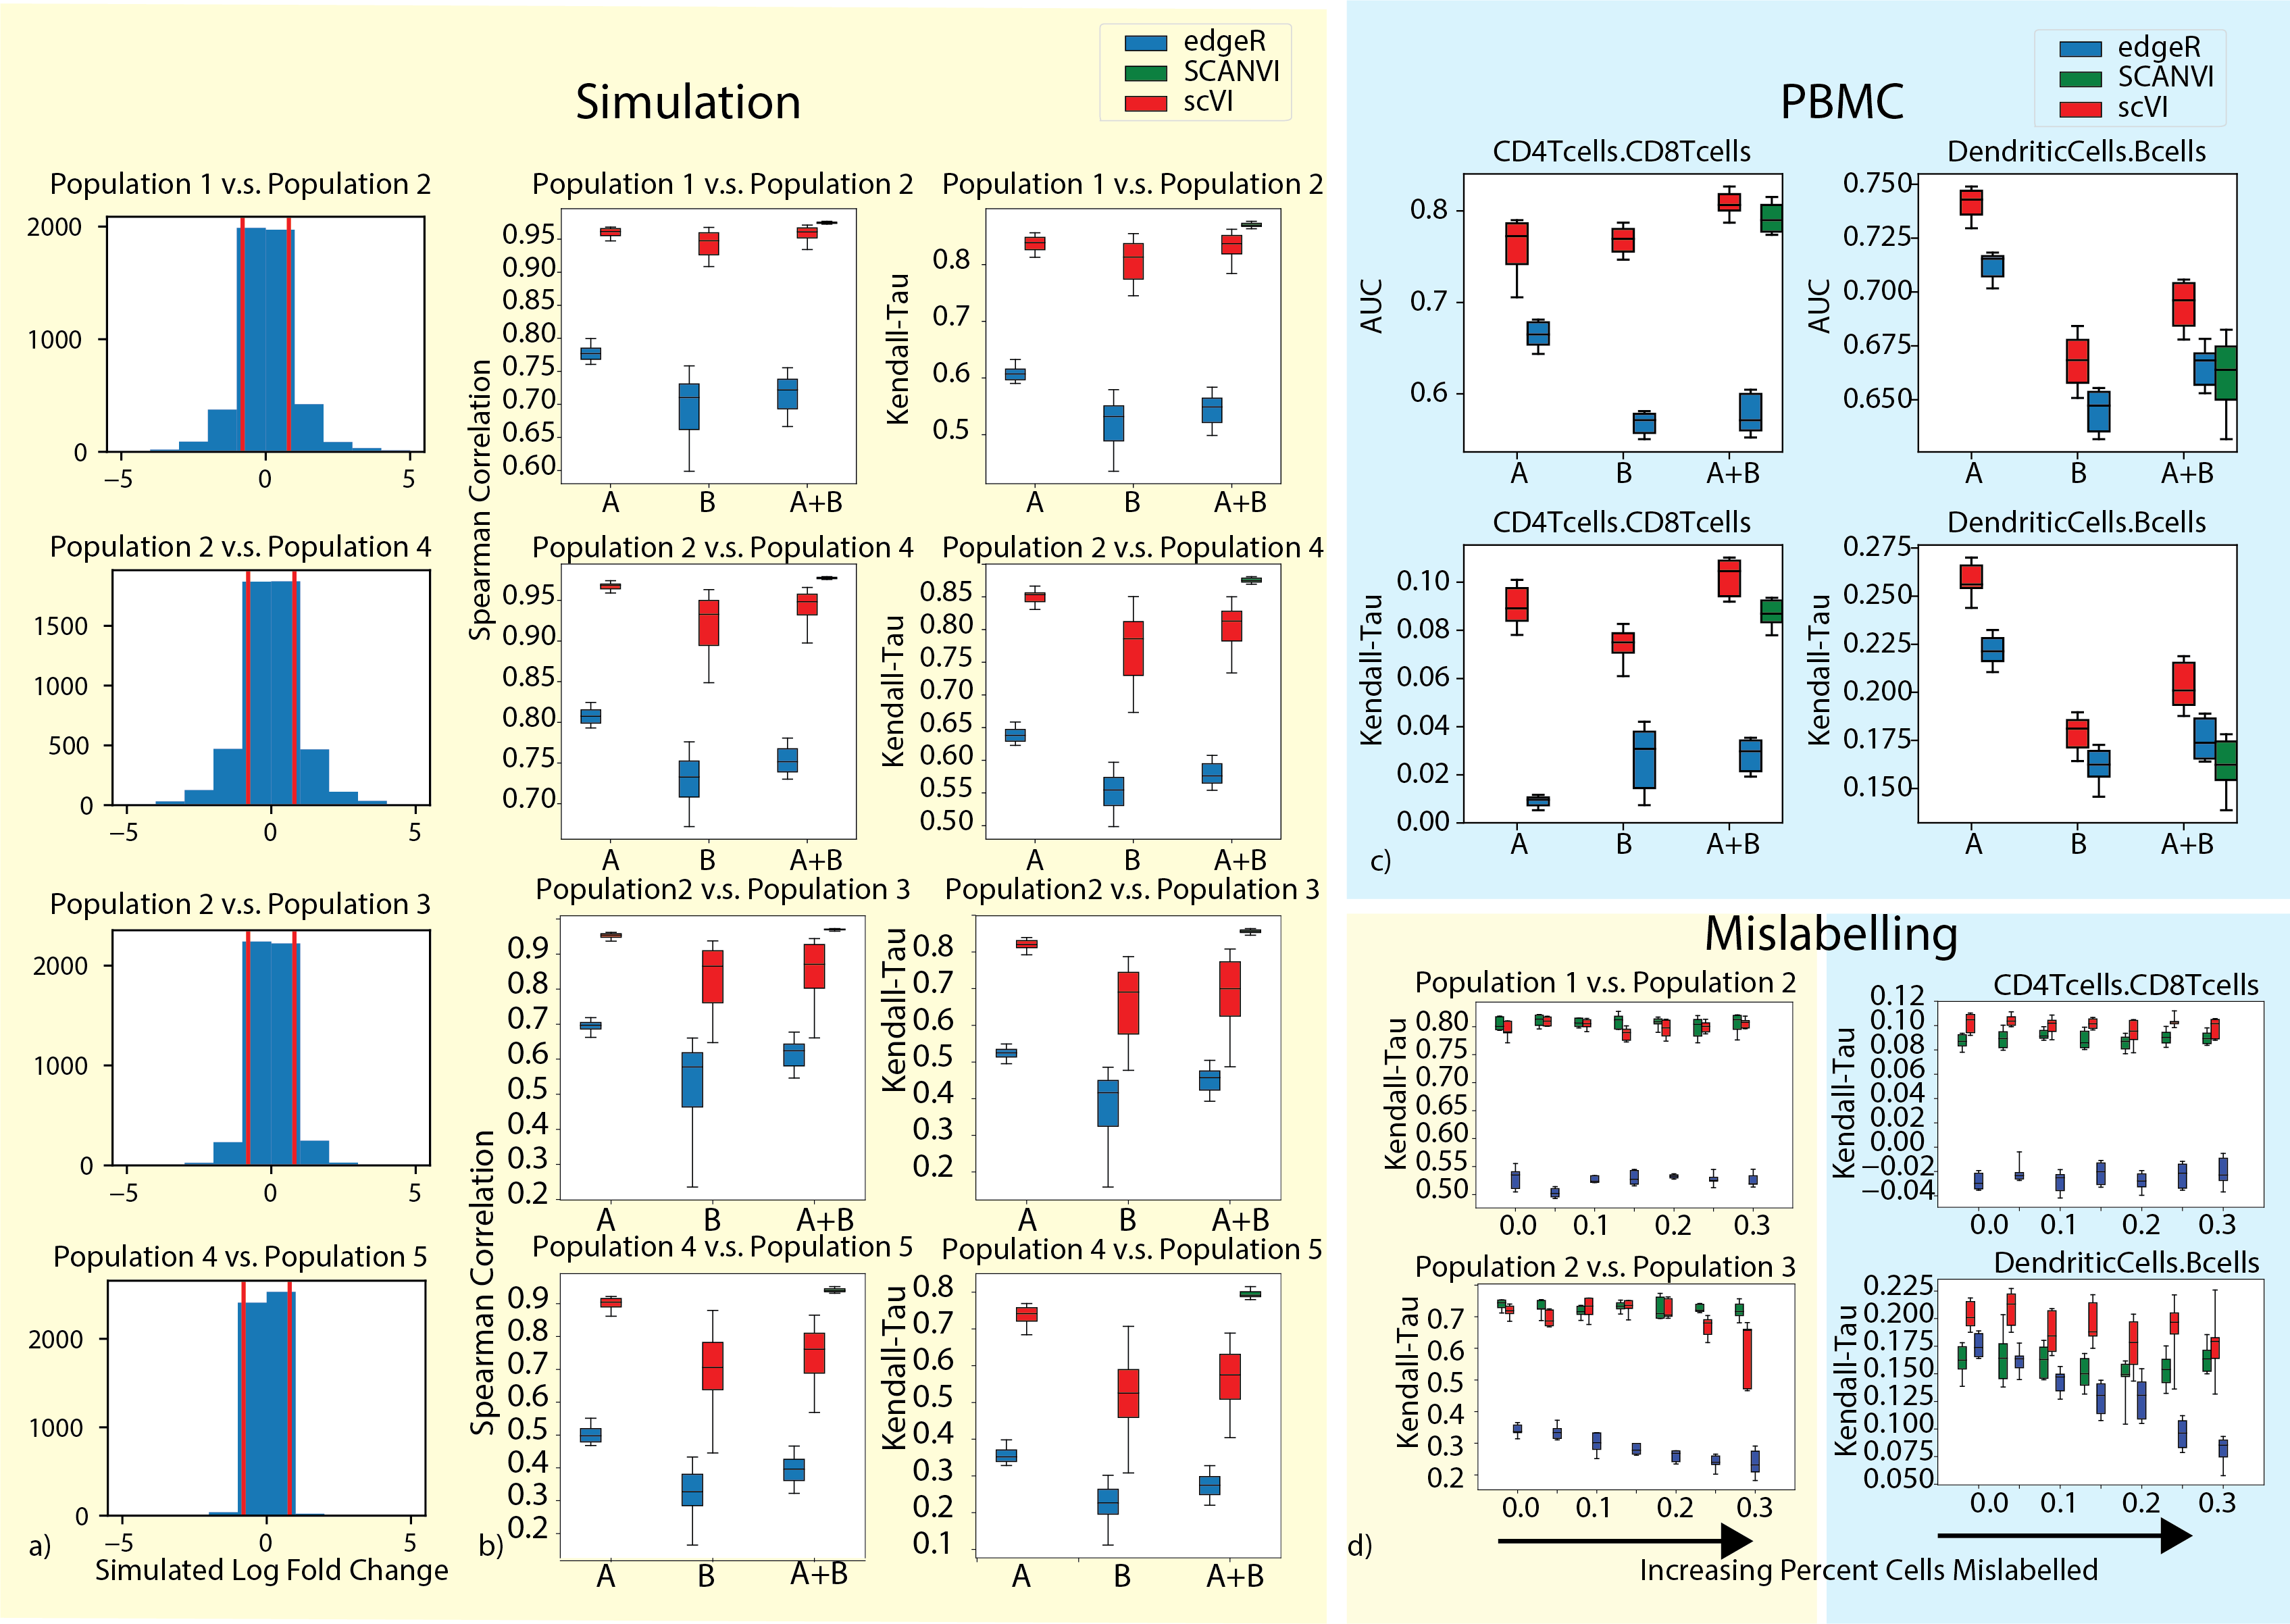
\includegraphics[width=0.8\textwidth]{figures/DE_maintext.png}
\caption[Differential Expression on multiple datasets with scVI]{Differential Expression on multiple datasets with scVI. $(a)$ distribution of true log fold change between all pairs of cell types for the simulated data. The pairs of cells are chosen to represent different levels of distance on the tree as in Figure~\ref{scanvisimulations_panel}a. The pairs of population from most distant to least distant are `12', `24', `23', `45'. 
$(b)$ Evaluation of consistency with rank correlation and Kendall-Tau is shown for comparisons of multiple pairs of cell types in the simulated data. 
$(c)$ Evaluation of consistency with the AUROC and Kendal Tau metric is shown for comparisons of CD4 vs CD8 T cells and B cells vs Dendritic cells on the PBMC-8K only (A), the PBMC-68k only (B) and the merged PBMC-8K / PBMC-68K (A+B) for scVI and edgeR. Error bars are obtained by multiple subsampling of the data to show robustness.  boxplots are standard Tukey boxplots where the box is delineated by the first and third quartile and the whisker lines are the first and third quartile plus minus 1.5 times the box height. The dots are outliers that fall above or below the whisker lines.
$(d)$ Mislabeling experiment in differential expression in both the SymSim simulated datasets and in the PBMC8K and PBMC68K dataset. The top row shows differential expression results for the correctly labeled population pair (Population 1 v.s. Population 2 in simulated dataset and CD4 T cells v.s. CD8 T cells in PBMC dataset. The bottom row shows differential expression results for the mislabelled population pair ( Population 2 v.s. Population 3 in simulated dataset and Dendritic Cells v.s. B cells in PBMC dataset). For all, x-axis represents the proportion of flipped labels. }
\label{scanvide_panel}
\end{figure}

With their probabilistic representation of the data, scVI and scANVI each provide a natural way of performing various types of hypotheses testing. This is different from other approaches~\cite{MNN,seurat,LIGER,scanorama,SEURAT3} where the dataset alignment procedures do not carry direct probabilistic interpretation, and the resulting harmonized data can thus not be directly used for these purposes.

\subsubsection{Bayesian differential expression with scANVI}
Contrary to scVI, scANVI doesn't need to rely on specific cells for differential expression since labels are given during the training. We still use the generative model but with the following probability for $p(\mathcal{H}_1^g \mid c_a, c_b)$ where $c_a$ (resp. $c_b$) is the first (resp. second) cell type of interest:
\begin{align}
p(\mathcal{H}_1^g \mid c_a, c_b) = \sum_s\int \mathds{1}_{f_w^g(z_a, s) \leq f_w^g(z_b, s) }p(s)dp(z_a \mid u_a, c_a)dp(z_b \mid u_b, c_b)dp(u_a)dp(u_b).
\end{align}
Notably, we draw here data from the prior distribution and not the posterior for given cells. As a consequence, these Bayes factors can be approximated in a unbiased fashion using a naive Monte Carlo estimator. We noticed in the case of the real dataset that the aggregate posterior on $u$ might not perfectly match the prior for rare cell types. Consequently, we replaced the prior by the aggregate posterior for all the analyses in this chapter. 

\subsubsection{Dataset}


To demonstrate this, we focus on the problem of differential expression. As a first case study, we use two of the PBMC datasets (PBMC-8K and PBMC-68K) and looked for differentially expressed genes in two settings: comparing the B cells to dendritic cells, and similarly for CD4$^+$ versus CD8$^+$ T cells. For evaluation, we used reference sets of differentially expressed genes that were obtained from published bulk-level analysis of similar cell subsets~(microarrays, \cite{Nakaya2011, Gorgun2005}, as in~\cite{scvi}). While this benchmark relies on real data, a clear caveat is the lack of a well defined ground truth. To address this, we used a second benchmark based on simulations with Symsim~\cite{symsim}. The simulated data consists of five subpopulations of varying degrees of transcriptional distance, profiled in two different “batches” of different technical quality (Figure~\ref{scanvisimulations_panel}). This framework allowed us to derive an exact log fold changes (LFC) between every pair of simulated subpopulations, which enable a more accurate evaluation of performance (Figure~\ref{scanvide_panel}a). 

In both benchmark studies, we assume that labels are only available for one of the two input batches or datasets (in the real data we assume that PBMC-8K is the annotated one). To apply scVI, we first harmonized the input pair of datasets and transferred labels using a $k$-nearest neighbors classifier on the joint latent space ($k=10$). We then consider these annotations (predicted and pre-labeled) as fixed and sample 100 cell pairs, each pair consisting of one cell from each population. For each cell pair we sample gene expression values from the variational posterior, while marginalizing over the different datasets, to compute the probability for differential expression in a dataset-agnostic manner. Aggregating across all selected pairs results in approximate Bayes factors that reflect the evaluated extent of differential expression. 

\subsubsection{Results}

For reference, we also included edgeR~\cite{edgeR} using the same labels as scVI. Notably, edgeR was shown to perform well on scRNA-seq data \cite{soneson2018bias} and uses a log-linear model to control for technical sample-to-sample variation.

In our simulations, we considered differential expression between every possible pair out of the five simulated subpopulations. For evaluation, we computed the Spearman and Kendall rank correlation coefficients between the true LFC and the inferred Bayes factors (for scVI and scANVI) or estimated LFC (for edgeR). Our results in (Figure~\ref{scanvide_panel}b) show that with this artificial, yet more clearly defined objective, scVI was substantially more accurate than edgeR and that in the harmonized data scANVI provided more exact and stable estimates than scVI. 

To evaluate performance on the real data, we defined genes as differentially expressed if the adjusted p-value in the reference bulk data (provided by~\cite{Nakaya2011, Gorgun2005}) was under $5 \%$. Considering these genes as positive instances, we calculated the area under the ROC curve (AUROC) based on rank ordering the inferred Bayes factors (for scVI and scANVI) or p-values (for edgeR). Since the definition of positives genes required a somewhat arbitrary threshold, we also used a second score that evaluates the reproducibility of gene ranking (bulk reference vs. single-cell; considering all genes), using the Kendall rank correlation coefficient (Figure~\ref{scanvide_panel}c). As a reference, we look at the accuracy of differential expression analysis in each PBMC dataset separately (using their prior annotations to define the sets of cells we are comparing), which can be computed with scVI (as in~\cite{scvi}) and edgeR. Reassuringly, we observe that the performance of scVI on the joint data is not lower than it is in either dataset in isolation. We also find that while scVI performs moderately better than scANVI, both methods compare favorably to edgeR in terms of accuracy. 

Mislabeling of a certain proportion of cells in a dataset is a plausible scenario that may occur in any study. An important challenge is therefore to maintain the validity of downstream analysis despite such “upstream” annotation errors.  To evaluate robustness in this setting, we repeated the simulation analysis, while introducing labeling errors at different rates. Specifically, prior to evaluating differential expression between two simulated sub-populations, we flip the labels of a certain proportion (up to $30\%$) of the respective cells in the annotated batch. We then proceed as before and assign labels to cells in the unannotated batch by scVI or scANVI, followed by differential expression analysis. Our results (Figure~\ref{scanvide_panel}d) suggest that scANVI is clearly more robust to this type of mislabeling than scVI (or edgeR, applied on the scVI- derived labels). Repeating the same analysis on the PBMC data (where the differential expression ground truth is obviously not available), we observe similar level of robustness in scANVI, albeit with not much difference compared to scVI and edgeR. 

Overall, our results demonstrate that both scVI and scANVI are capable of conducting differential expression effectively, while working directly on a harmonized dataset. Furthermore, we observe that both methods and especially scANVI are robust to mislabeling, providing further motivation for explicitly modeling label uncertainty.

\section{Discussion}
In this study, we demonstrated that scVI provides a principled approach to harmonization  of scRNA-seq data through joint probabilistic representation of multiple dataset, while accounting for technical hurdles such as variable library size and limited sensitivity. We have demonstrated that scVI compares favorably to other methods in its accuracy and that it scales well, not only in terms of the number of cells (as in~\cite{scvi}) but also the number of input datasets (as opposed to other methods that work in a pairwise fashion and therefore scale quadratically with dataset size \cite{scanorama}). We have also shown that the harmonization step of scVI provides an effective baseline for automated transfer of cell type labels, from annotated datasets to new ones. 

While the performance of scVI in the annotation problem compares favorably to other algorithms, it does not make use of any existing cell state annotations during model training, but rather after the latent space has been learned. To make better use of these annotations (which may be available for only some of the input datasets or only some cells within a dataset), we developed scANVI, a semi-supervised variant of scVI. While the latent space of scVI is defined by a Gaussian vector with diagonal unit variance, scANVI uses a mixture model, which enables it to directly represent the different cell states (each corresponding to a mixture component) and provide a posterior probability of associating each cell with each label. We have demonstrated that similar to scVI, scANVI is capable of harmonizing datasets effectively. In addition, scANVI provides a way to address a number of variants of the annotation problem. Here, we have first shown that it performs well in the most prevalent application of transferring labels from a reference dataset to an unannotated one. We then demonstrated that scANVI can be used in the context of a single unannotated dataset, where high confidence (``seed'') labels are first inferred for a few cells (using marker genes) and then propagated to the remaining cells. Finally, we have shown that scANVI is especially useful in the challenging case where the differences between cell states are too subtle to be captured clearly by a transcriptome-wide similarity measure, as well as in the case where the labels are organized in a hierarchy. 

Notably, although scANVI achieves high accuracy when transferring labels from one dataset to another, it was not designed to automatically identify previously unobserved labels. Indeed, in Figure~\ref{scanviNclasses} we demonstrate that increasing the number of labels in the model ($C$) to values beyond the number of observed labels does not alter the results much. Nevertheless, we observed that unannotated cell populations that have an unobserved label are associated with low levels of mixing between the input datasets. We therefore advocate that clusters from an unannotated dataset that do not mix well should be inspected closely and, if appropriate, should be manually assigned with a new label.

One concern in applying methods based on neural networks~\cite{saucie, scvis,VASC,dca,scVAE} in single-cell genomics and other domains is the robustness to hyperparameters choices~\cite{tybalt_param}. This concern has been addressed to some extent by recent progress in the field, proposing search algorithms based on held-out log-likelihood maximization~\cite{dca}. In this chapter, we used an alternative approach that is more conducive for direct and easy application of our methods --- namely we fix the hyperparameters and achieve state-of-the-art results on a substantial number of datasets and case studies. 

The development of scVI and scANVI required several modeling and implementation choices. In Figures~\ref{scanviZINB_NB} and~\ref{scanviDE_NB} we discuss the rationale behind the choice of a zero-inflated negative binomial (ZINB) distribution as well as robustness to choice of priors. Briefly, we find that exclusion of zero inflation from the model results in approximately similar performance, which is consistent with findings in \cite{hafemeister2019normalization, townes2019feature}. The only exception is the case of harmonizing Smart-Seq2 and 10x data sets, in which ZINB performs significantly better. Such results might suggest that zero-inflation may be more suitable for certain technologies than others. Similarly, we investigate the prior on the library size which is defined per batch and show that computing the same prior for both the datasets (rather than each dataset individually, as we do by default) affects the performance only in the case of harmonizing the same pair of Smart-Seq2 and 10x datasets. Since these datasets have very different sources of technical noise, this may suggest that it is indeed advisable to explicitly account for such differences during model fit.

An important distinguishing feature of both scVI and scANVI is that they rely on a fully-probabilistic model, thus providing a way to directly propagate uncertainties to any downstream analysis. While we have demonstrated this for differential expression analysis and cell type annotation, this can be incorporated to other tasks, such as differential abundance of sub-populations in case-control studies, correlation between genes and more. We therefore expect scVI, scANVI and similar tools to be of much interest as the field moves toward the goal of increasing reproducibility and consistency between studies and converging on to a common ontology of cell types. In particular, we expect scANVI to be especially useful for transferring labels while taking into account the uncertainty, or in the case of a more complex label structure such as hierarchical cell types. Finally, as recent preprints propose proof of concepts for integrating single cell data across different data modalities such as Single molecule fluorescent in situ hybridization (smFISH), RNA-seq, ATAC-seq and DNA methylation~\cite{LIGER, SEURAT3}, further work can utilize probabilistic graphical models that quantify measurement uncertainties in each assay, as well as the uncertainties of transferring information between modalities (e.g., predicting unmeasured gene expression in smFISH data as in~\cite{DBLP:journals/corr/abs-1905-02269}).




\section{Supplementary figures}


\begin{suppfigure}[H]
\centering
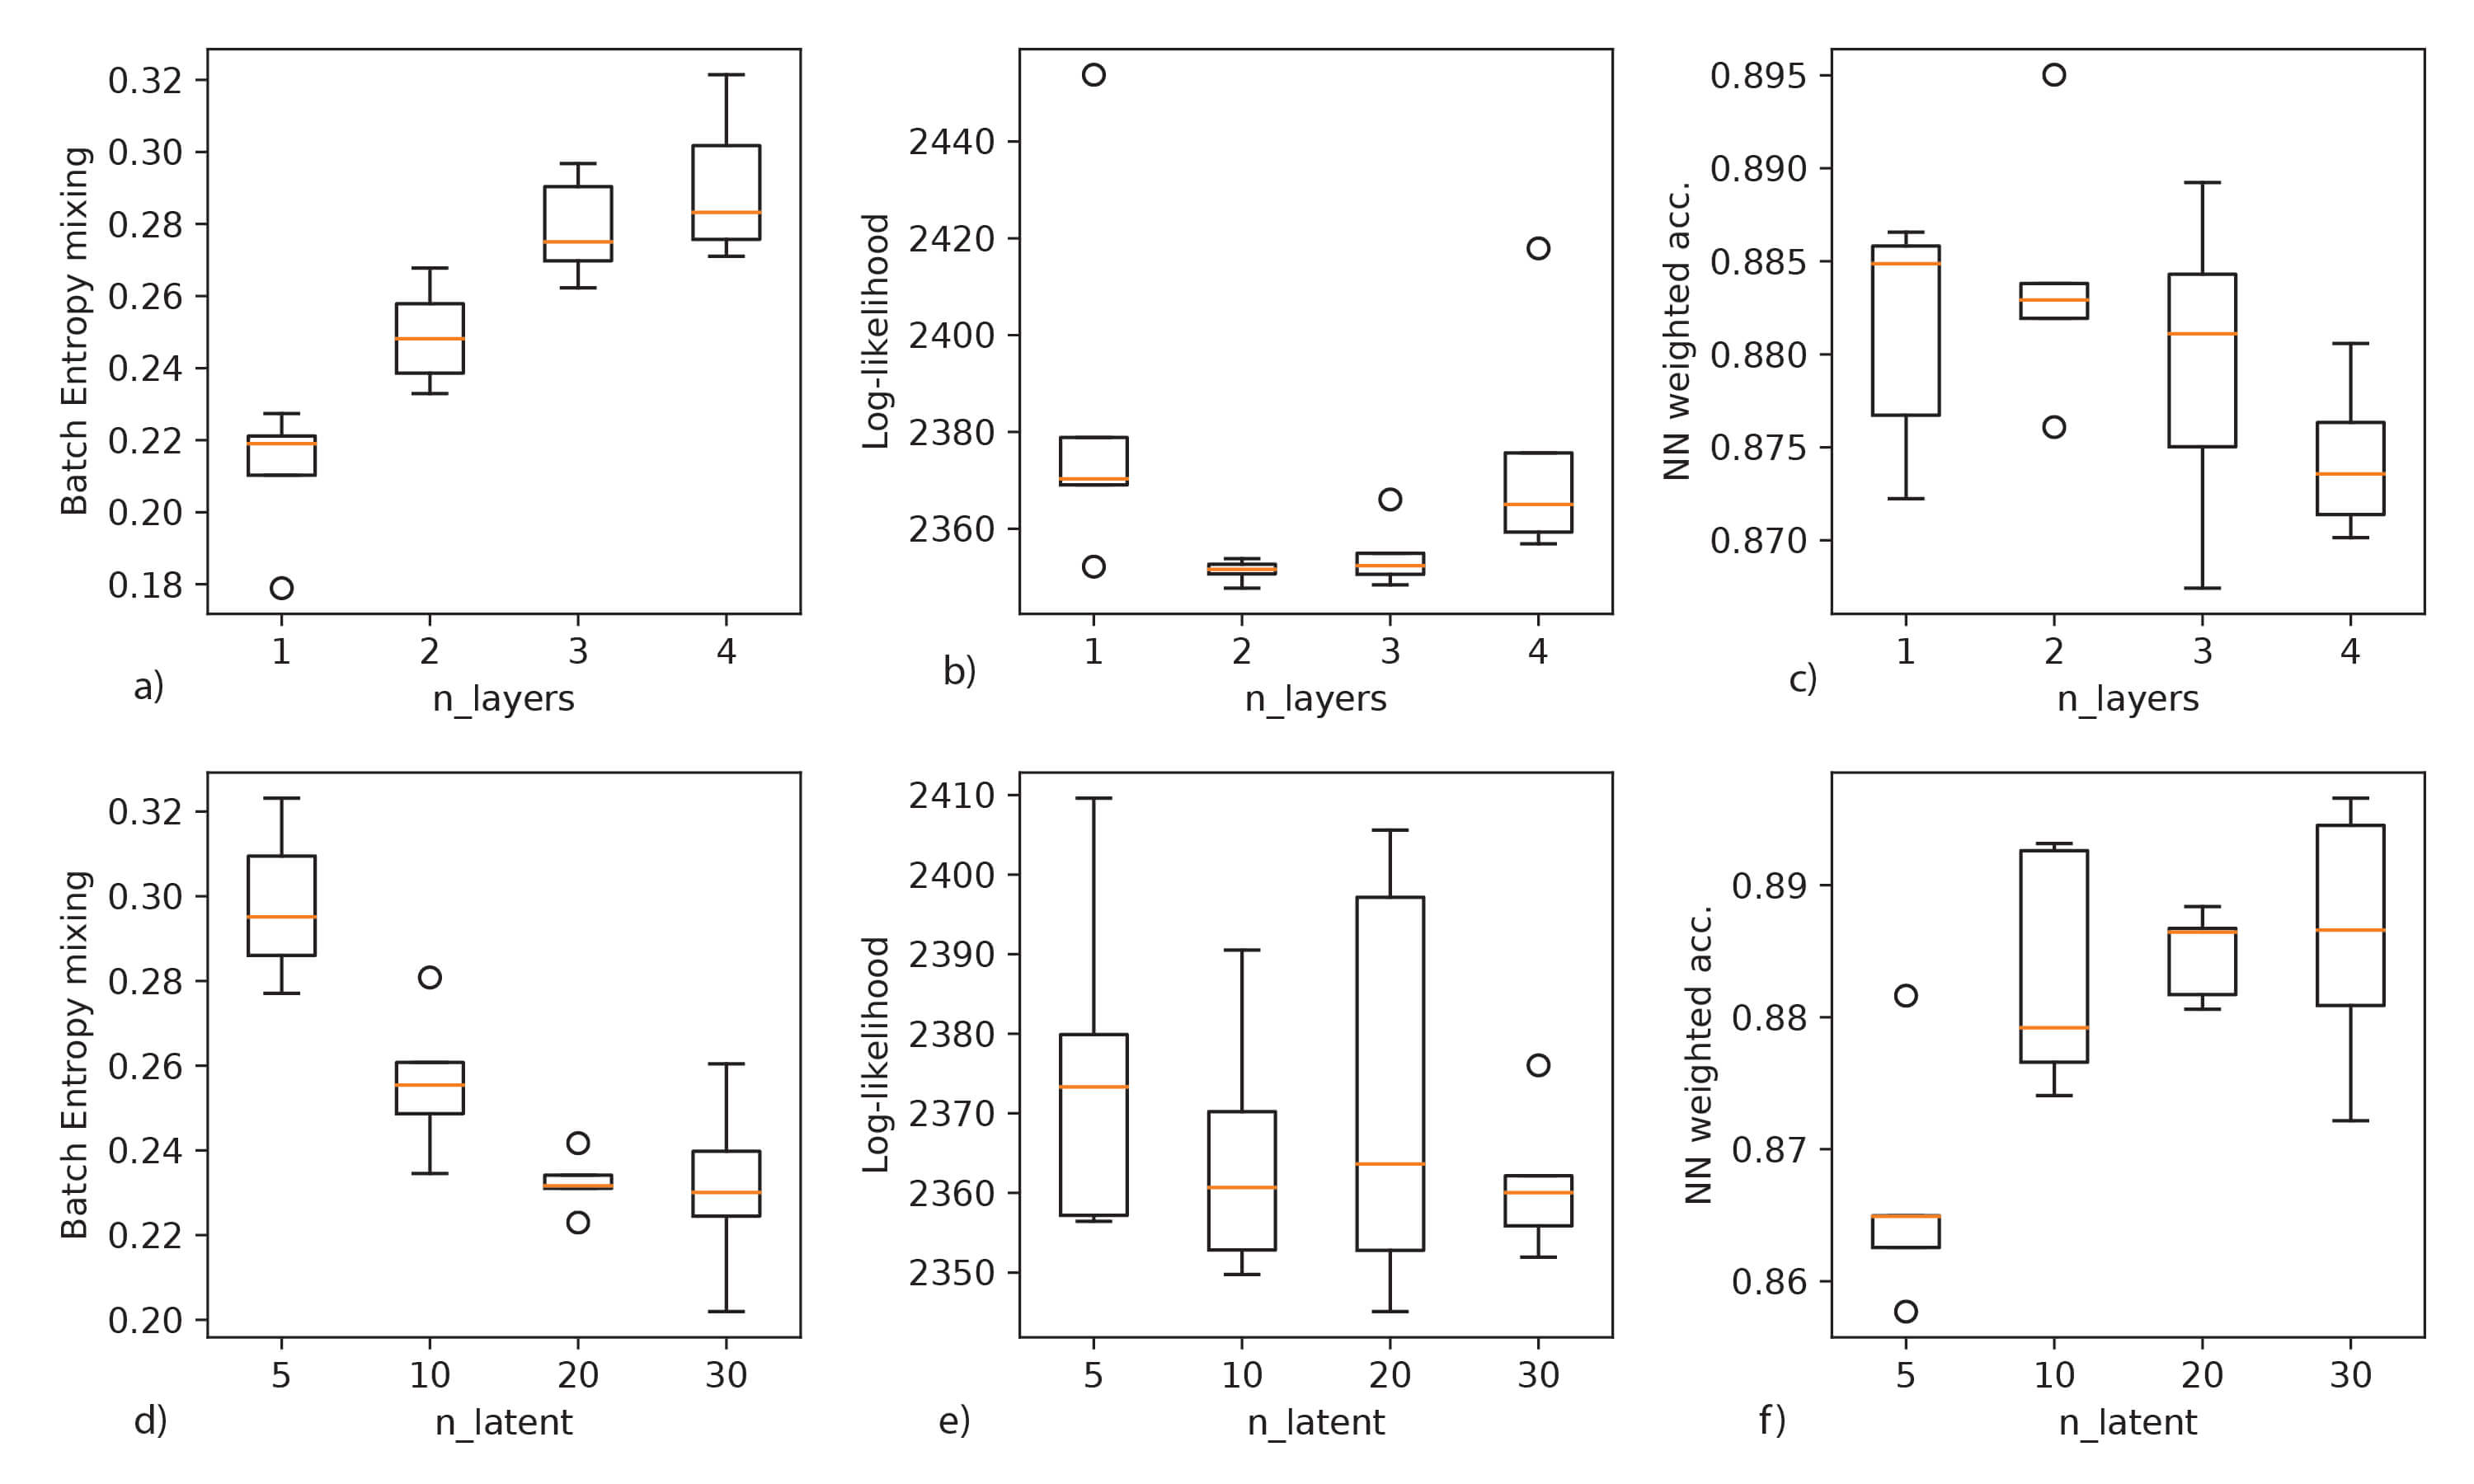
\includegraphics[width=\textwidth]{figures/robust.jpg}
\caption[Robustness analysis for harmonization of the pair of datasets MarrowMT-10x / MarrowMT-ss2 with scVI]{Robustness analysis for harmonization of the pair of datasets MarrowMT-10x / MarrowMT-ss2 with scVI. $(a-c)$ We augment the number of hidden layers in the neural network $f_w$ and track across $n=5$ random initializations for the batch entropy mixing $(a)$, the held-out log likelihood $(b)$ and the weighted accuracy of a nearest neighbor classifier on the latent space $(c)$. $(d-f)$ We increase the number of dimensions for the latent variable $z$ and track across $n=5$ random initialization the batch entropy mixing $(d)$, the held-out log likelihood $(e)$ and the weighted accuracy of a nearest neighbor classifier on the latent space $(f)$.}
\label{scanvirobustness_supplement}
\end{suppfigure}

\begin{suppfigure}[H]
    \centering
    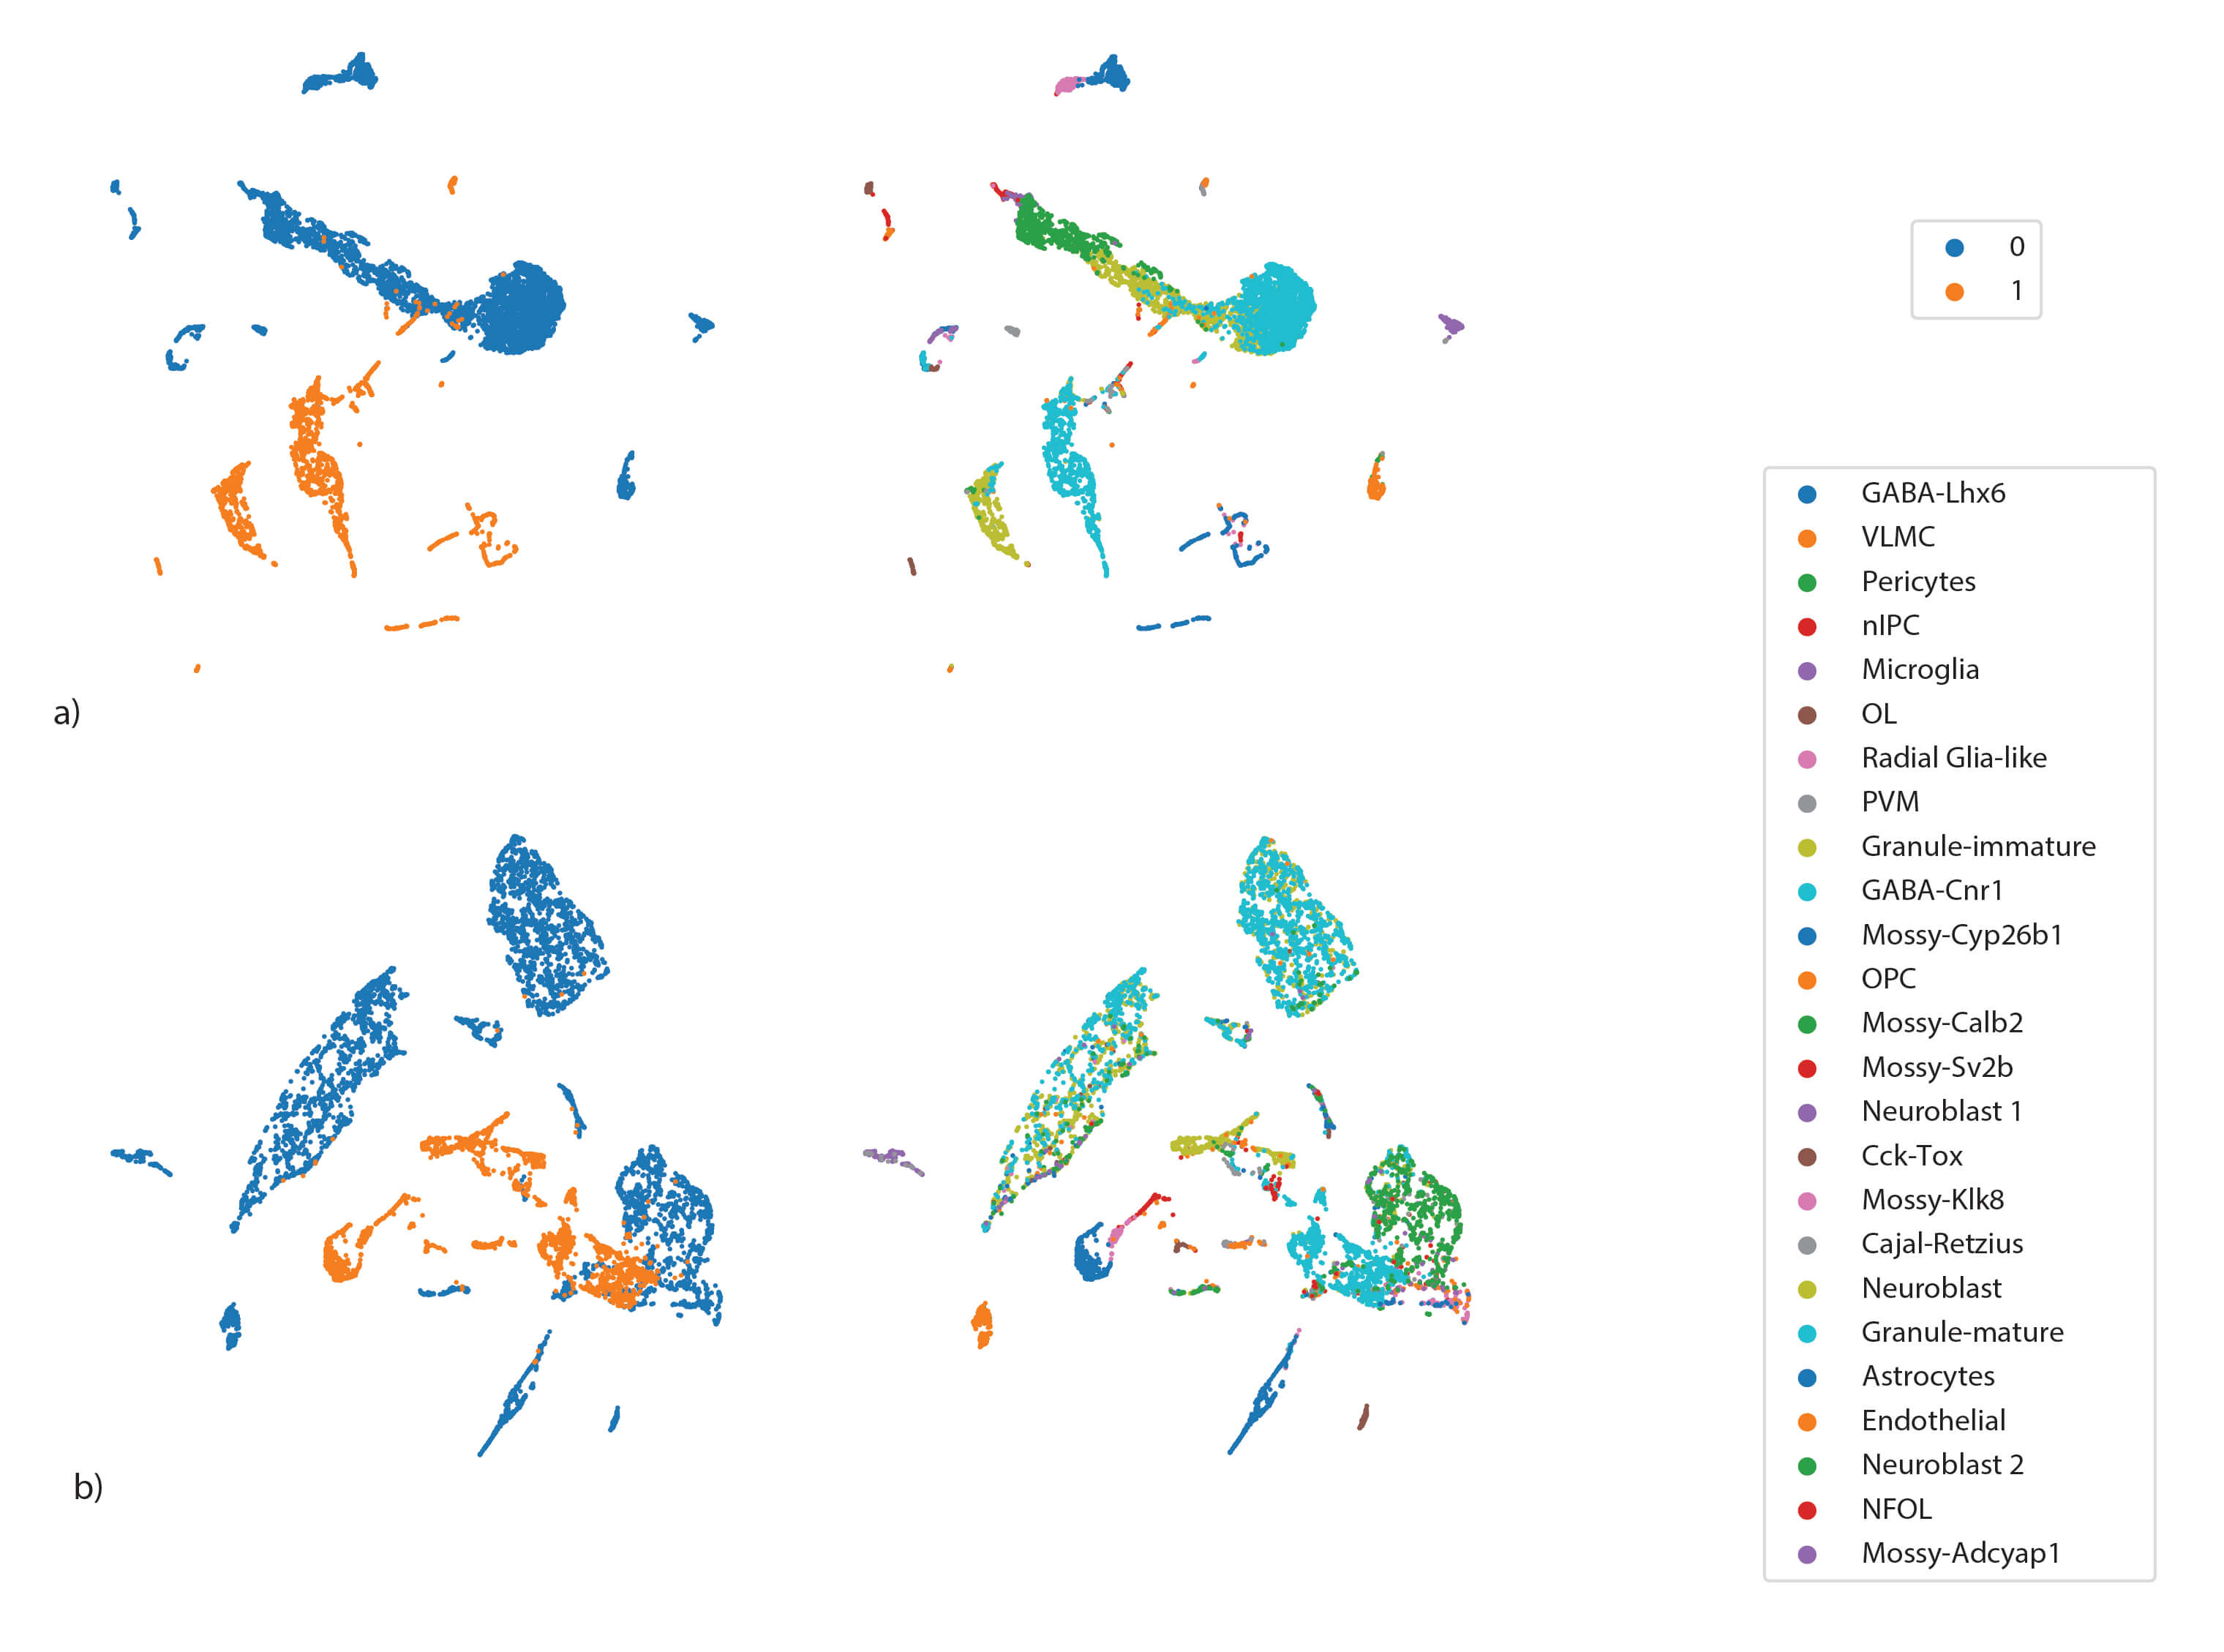
\includegraphics[width=\textwidth]{figures/magan.jpg}
    \caption[Visualization of the output of MAGAN on the DentateGyrus pair of datasets.]{Visualization of the output of MAGAN on the DentateGyrus pair of datasets. Using MAGAN, we projected the first dataset into the second one $(a)$ and vice-versa $(b)$. }
    \label{scanvimagan}
\end{suppfigure}

\begin{suppfigure}[H]
\centering
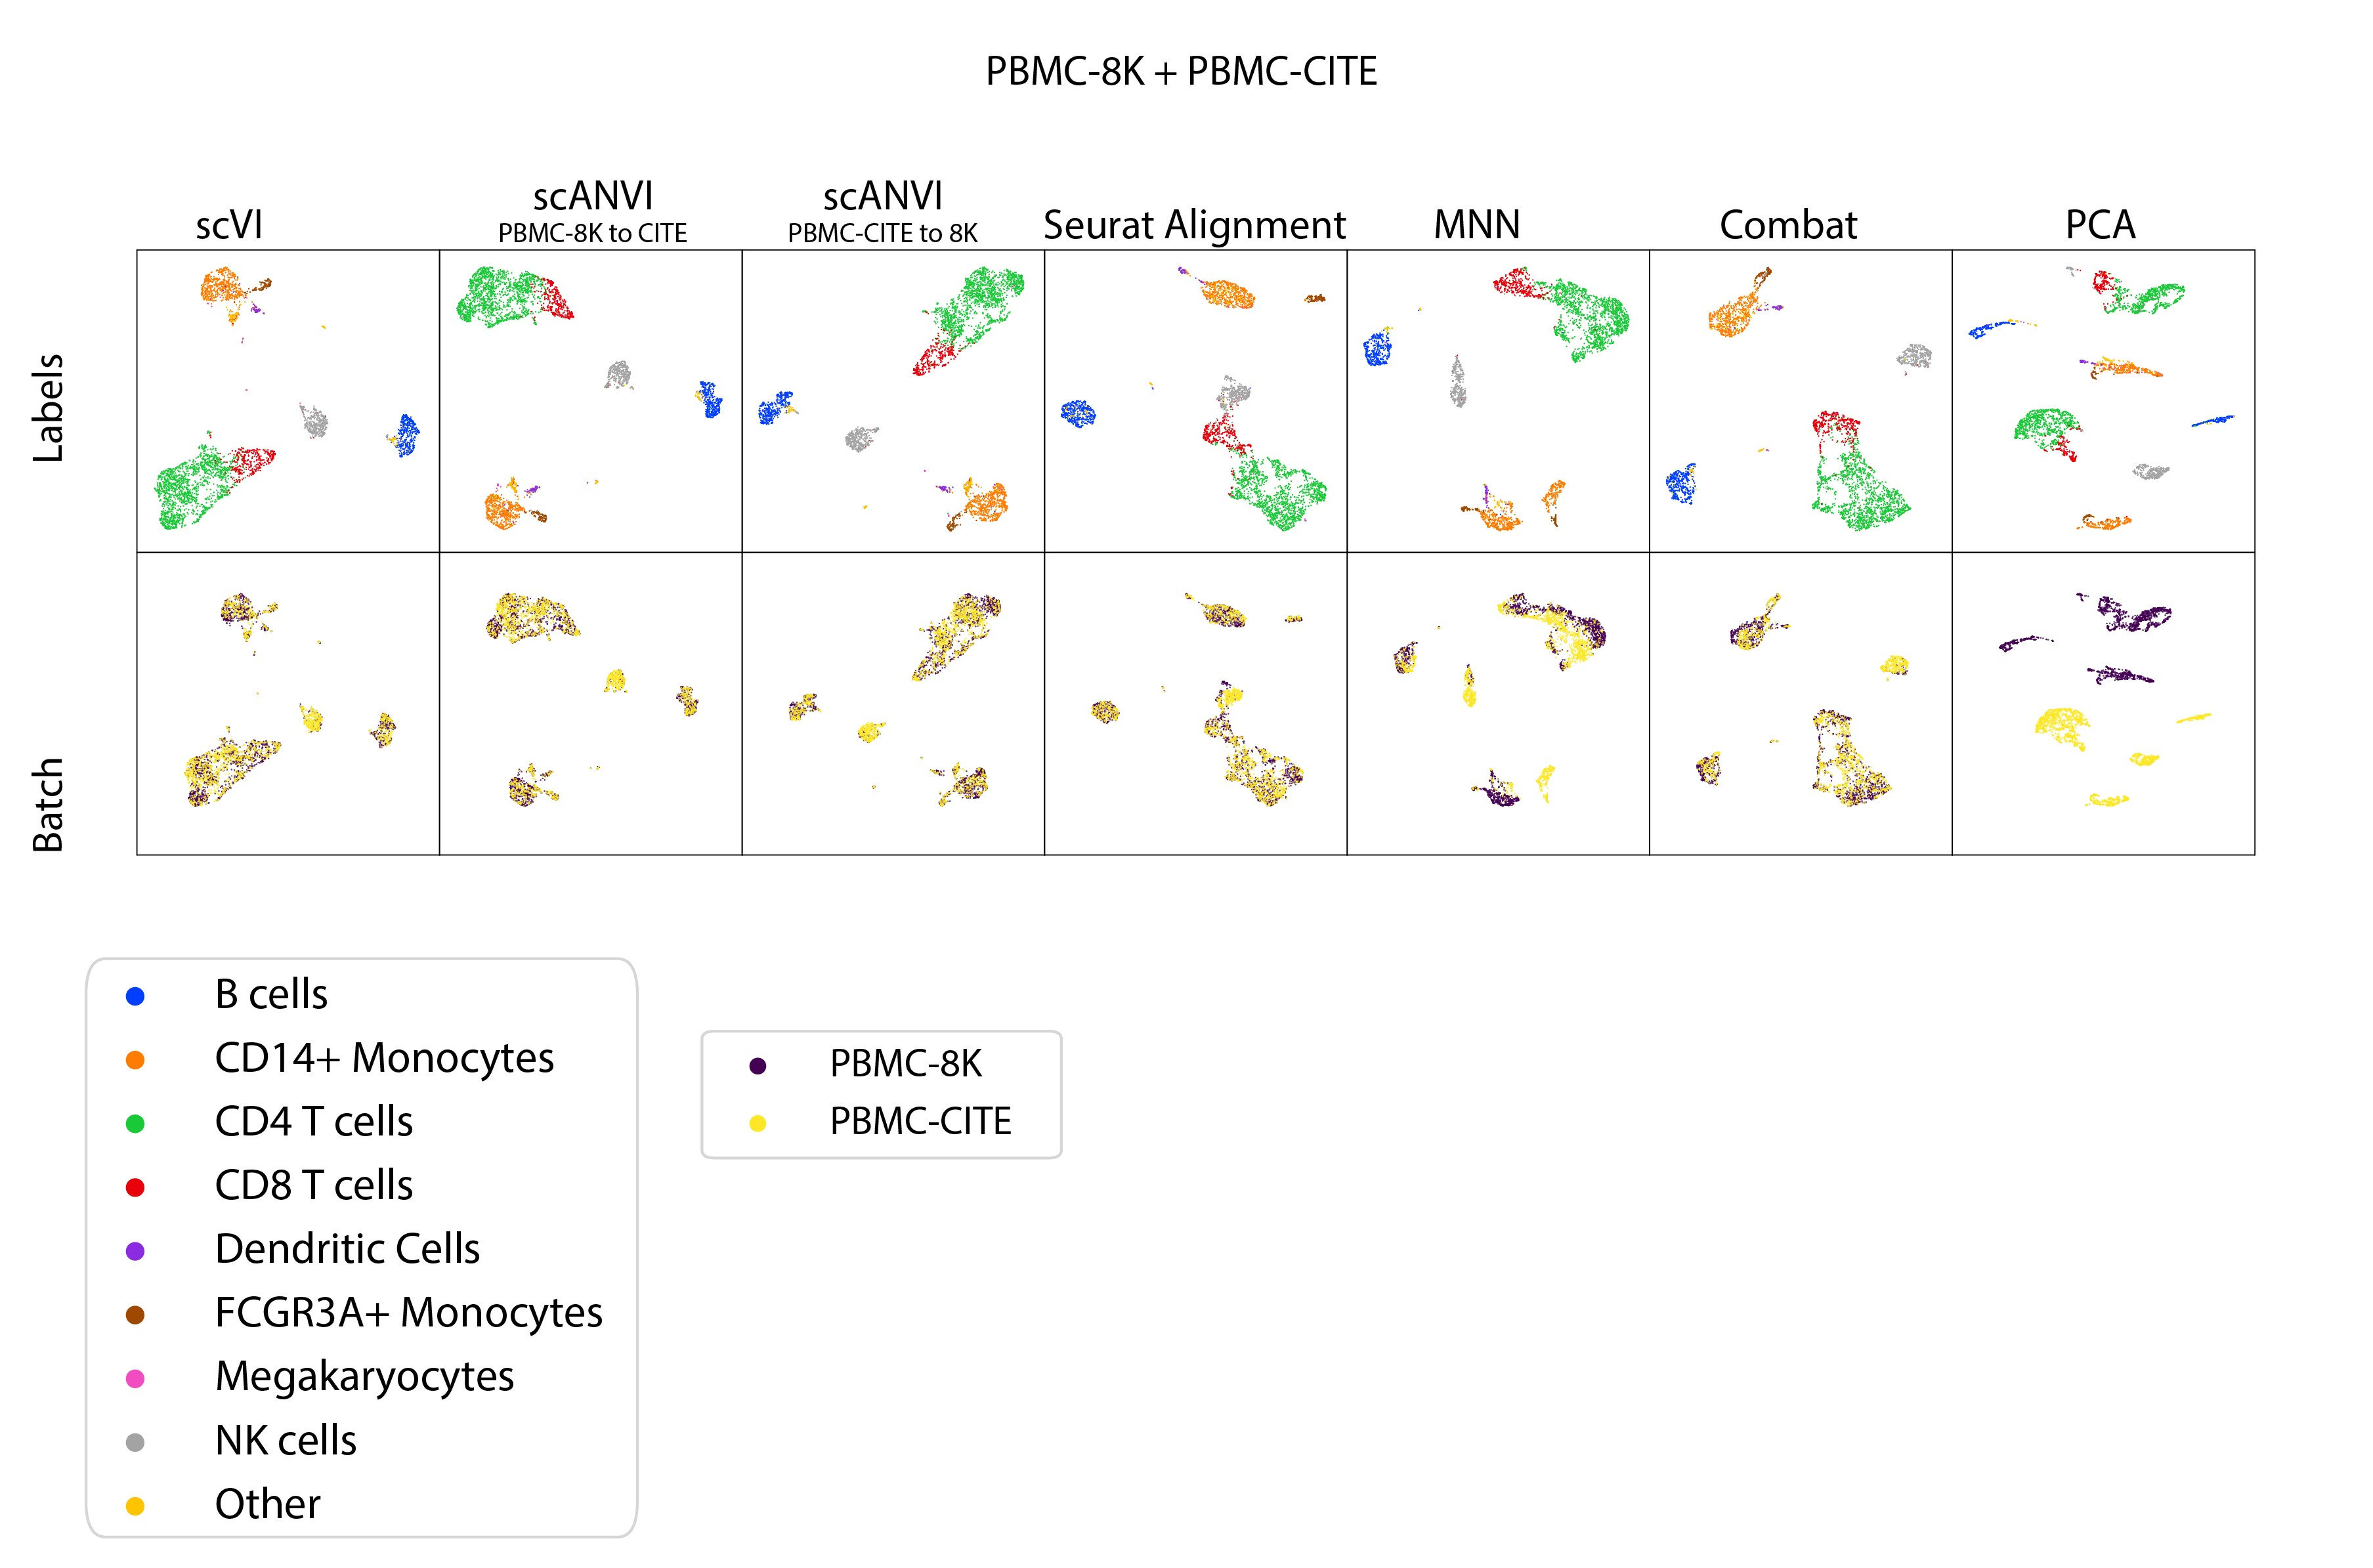
\includegraphics[width=\textwidth]{figures/supFig1-Easy1.jpg}
\caption[Visualization of the benchmark PBMC-8K / PBMC-CITE.]{Visualization of the benchmark PBMC-8K / PBMC-CITE. All positions for the scatter plots are derived using UMAP on the latent space of interest.}
\label{scanviEasy1}
\end{suppfigure}



\begin{suppfigure}[H]
\centering
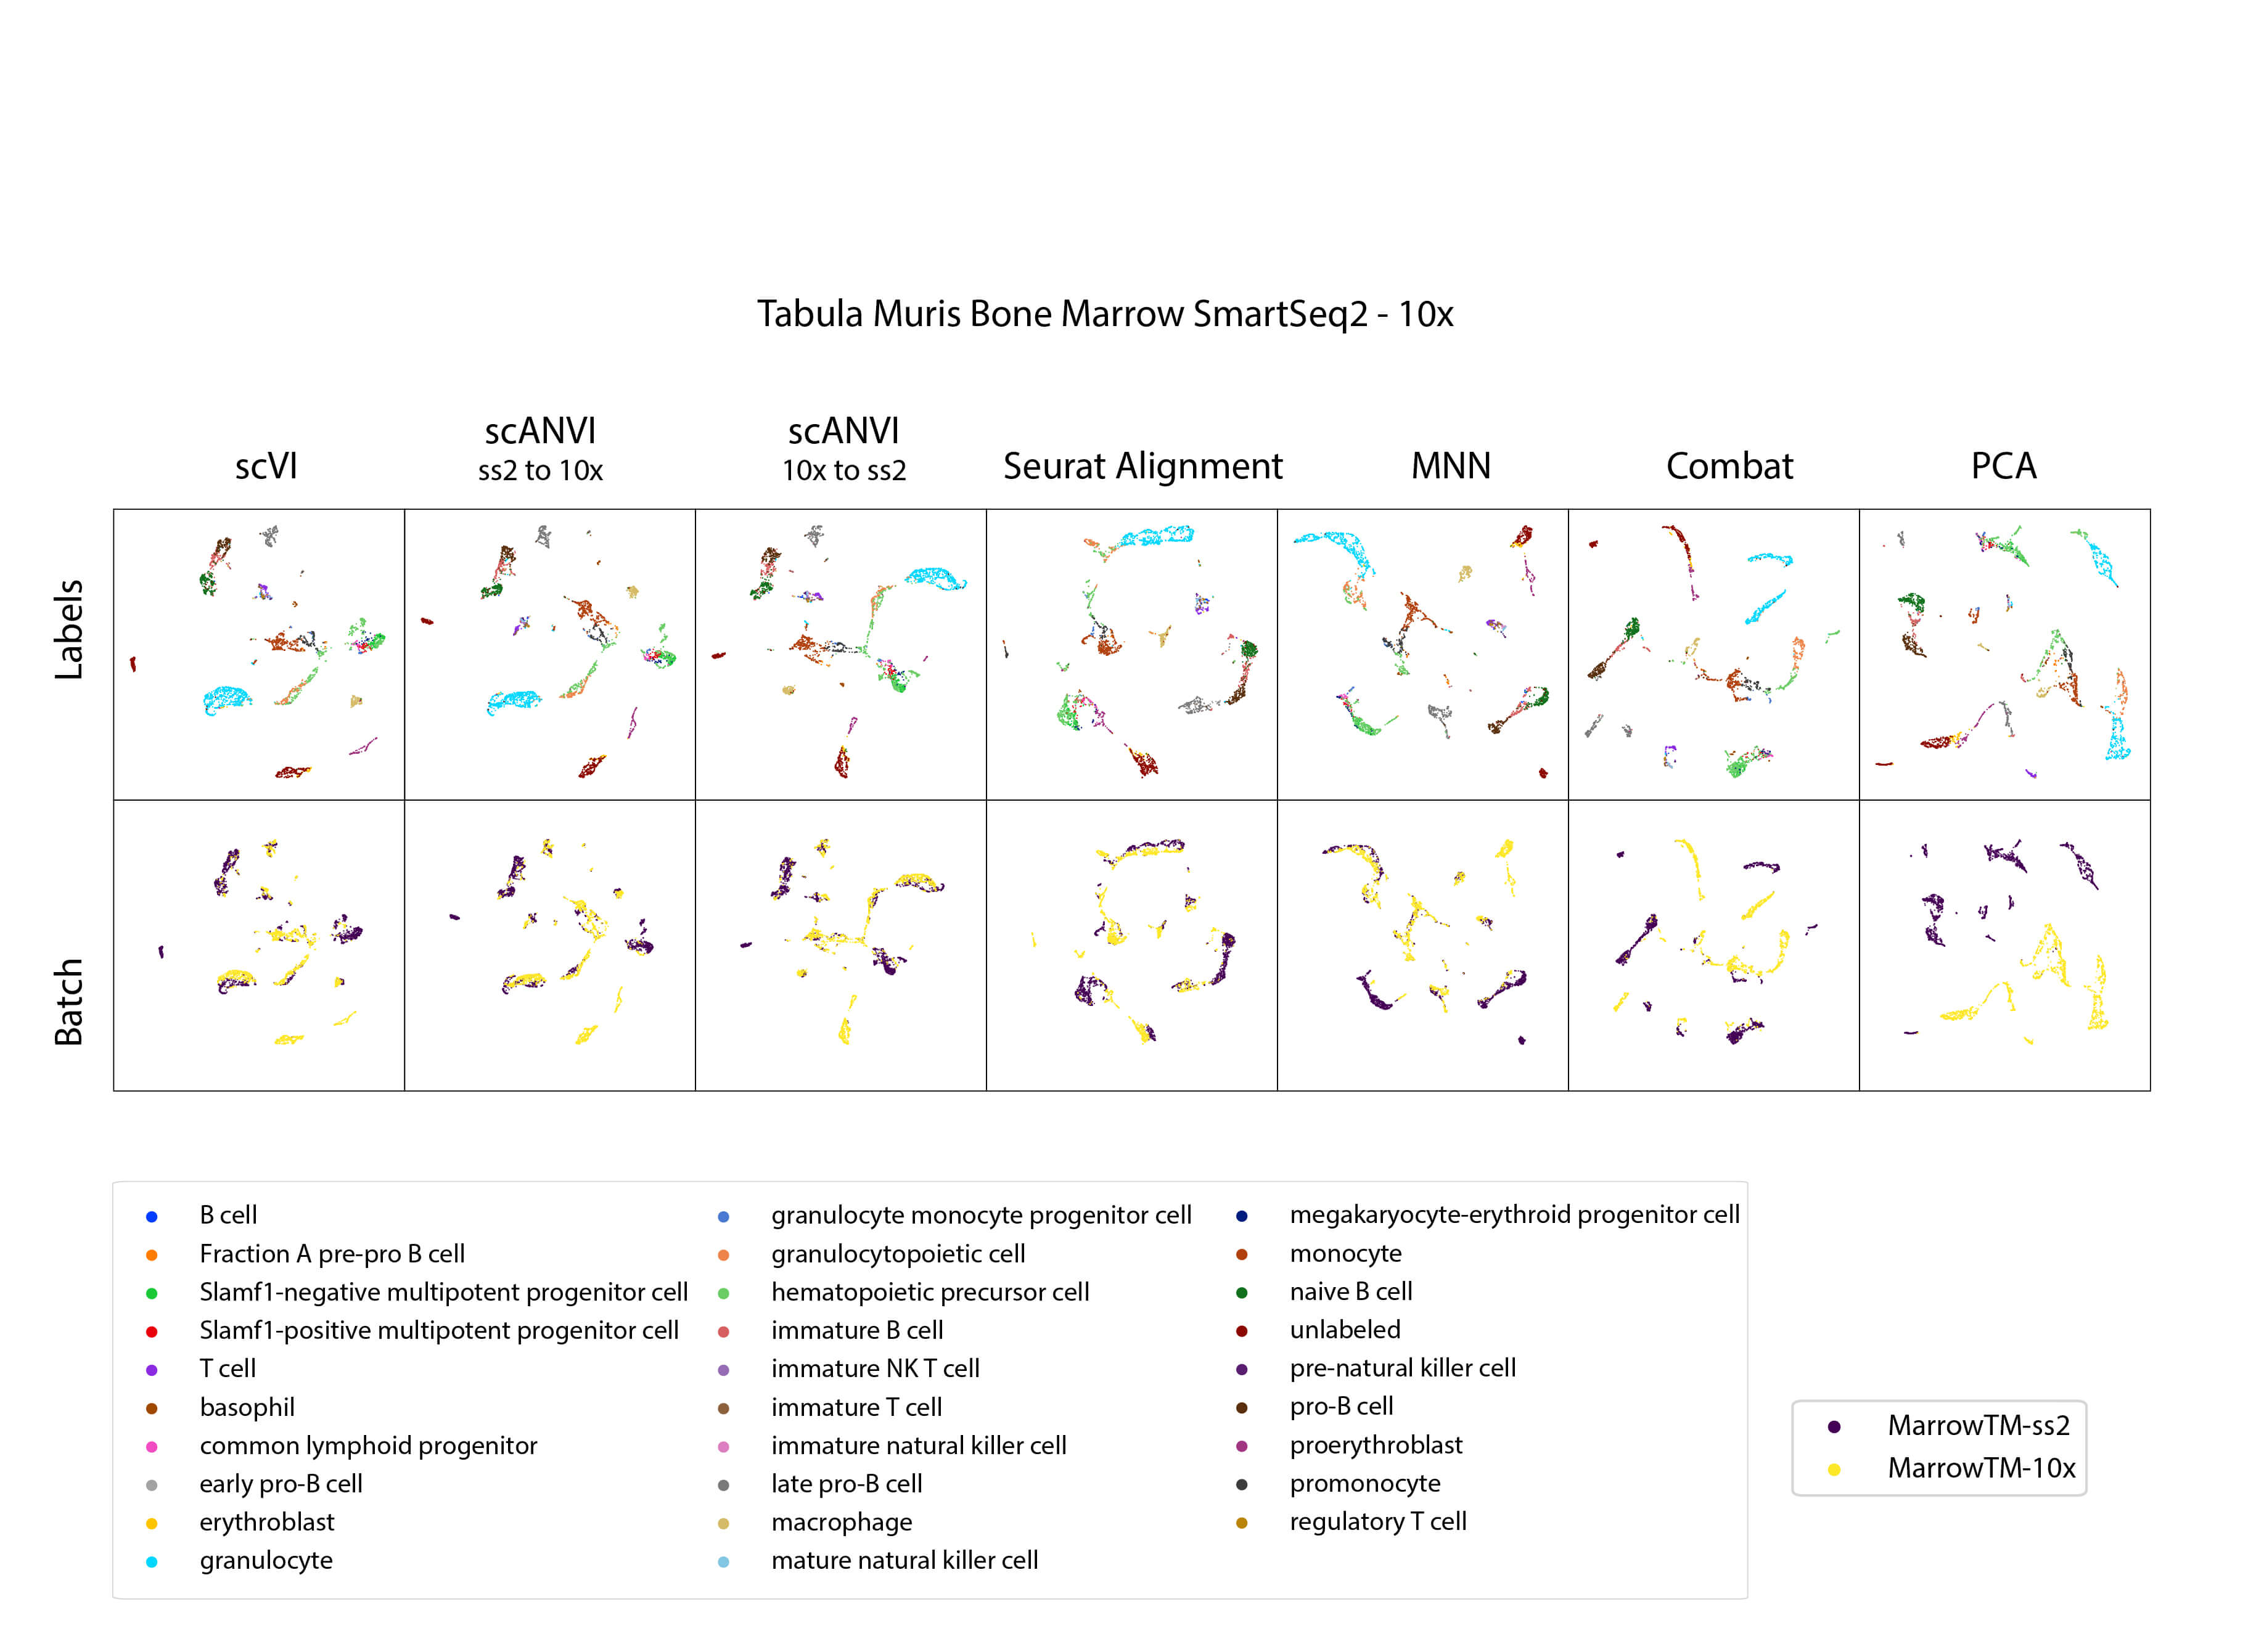
\includegraphics[width=\textwidth]{figures/supFig1-Tech1.jpg}
\caption[Visualization of the benchmark MarrowMT 10x / ss2.]{Visualization of the benchmark MarrowMT 10x / ss2. All positions for the scatter plots are derived using UMAP on the latent space of interest.}
\label{scanviTech1}
\end{suppfigure}


\begin{suppfigure}[H]
\centering
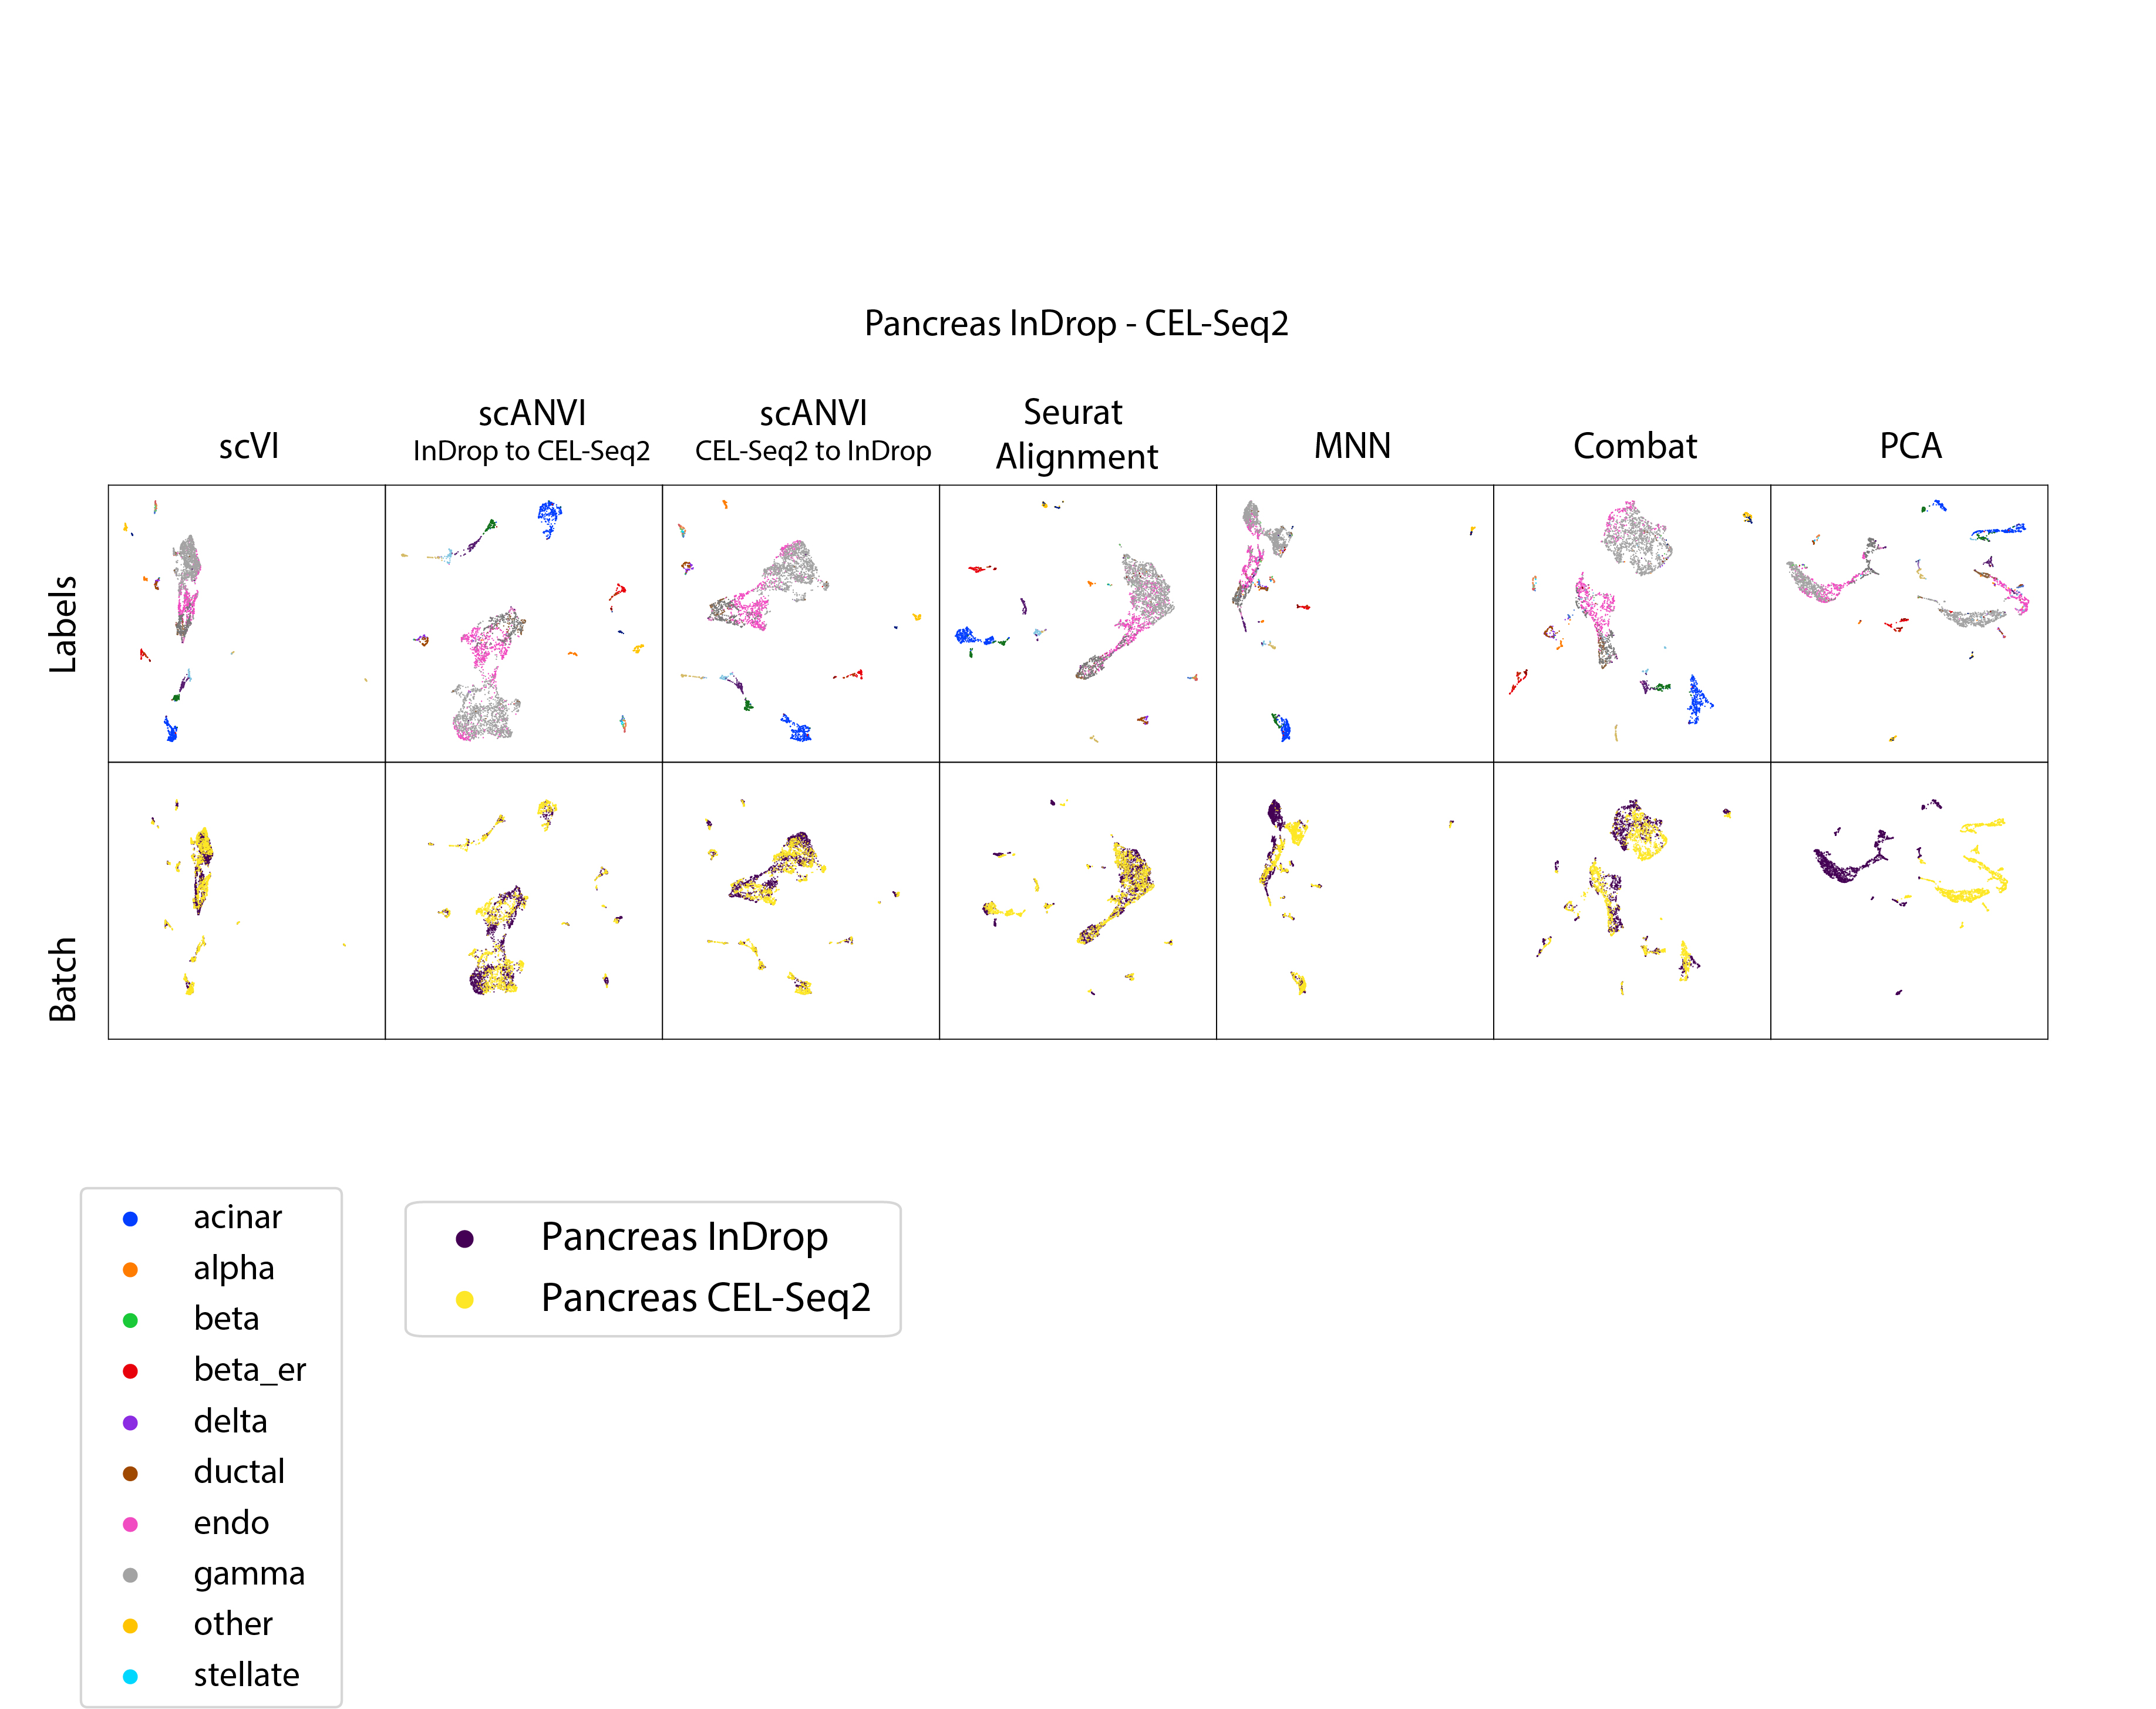
\includegraphics[width=\textwidth]{figures/supFig1-Tech3.jpg}
\caption[Visualization of the benchmark Pancreas InDrop / CEL-Seq2]{Visualization of the benchmark Pancreas InDrop / CEL-Seq2. All positions for the scatter plots are derived using UMAP on the latent space of interest.}
\label{scanviTech3}
\end{suppfigure}


\begin{suppfigure}[H]
\centering
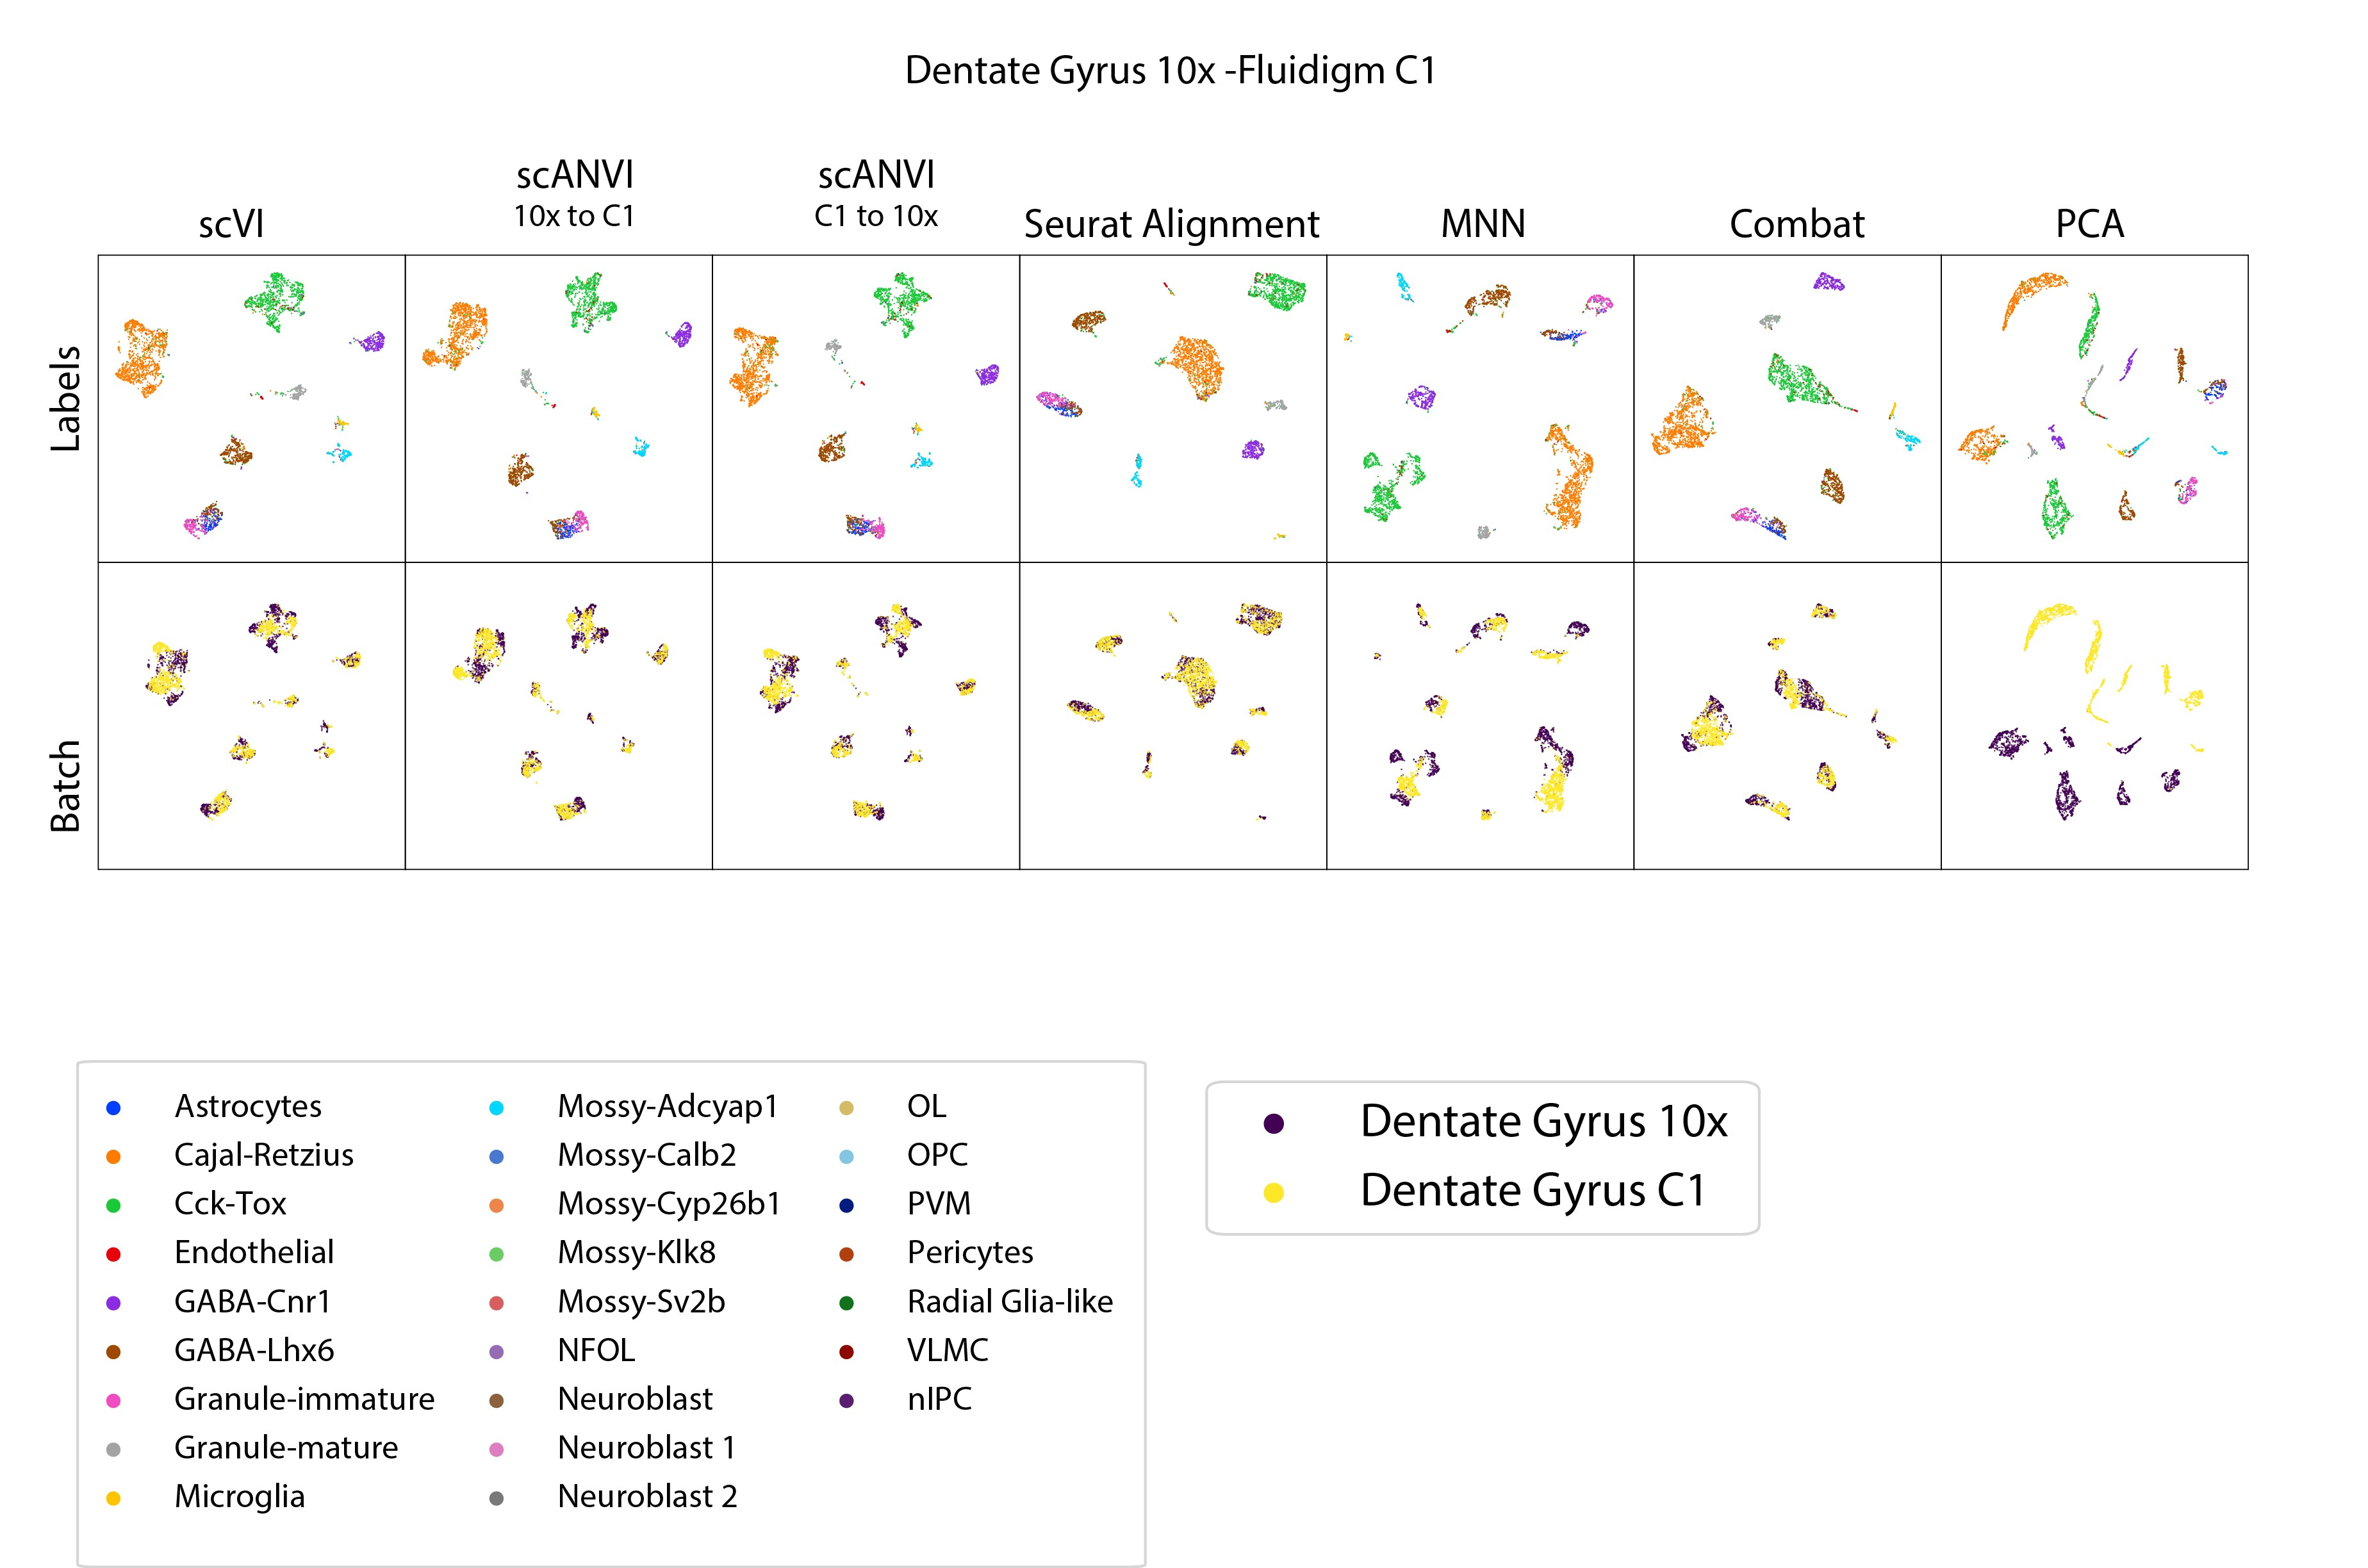
\includegraphics[width=\textwidth]{figures/supFig1-Tech4.jpg}
\caption[Visualization of the benchmark DentateGyrus10X - Fluidigm C1]{Visualization of the benchmark DentateGyrus10X - Fluidigm C1. All positions for the scatter plots are derived using UMAP on the latent space of interest.}
\label{scanviTech4}
\end{suppfigure}



\begin{suppfigure}[H]
    \centering
    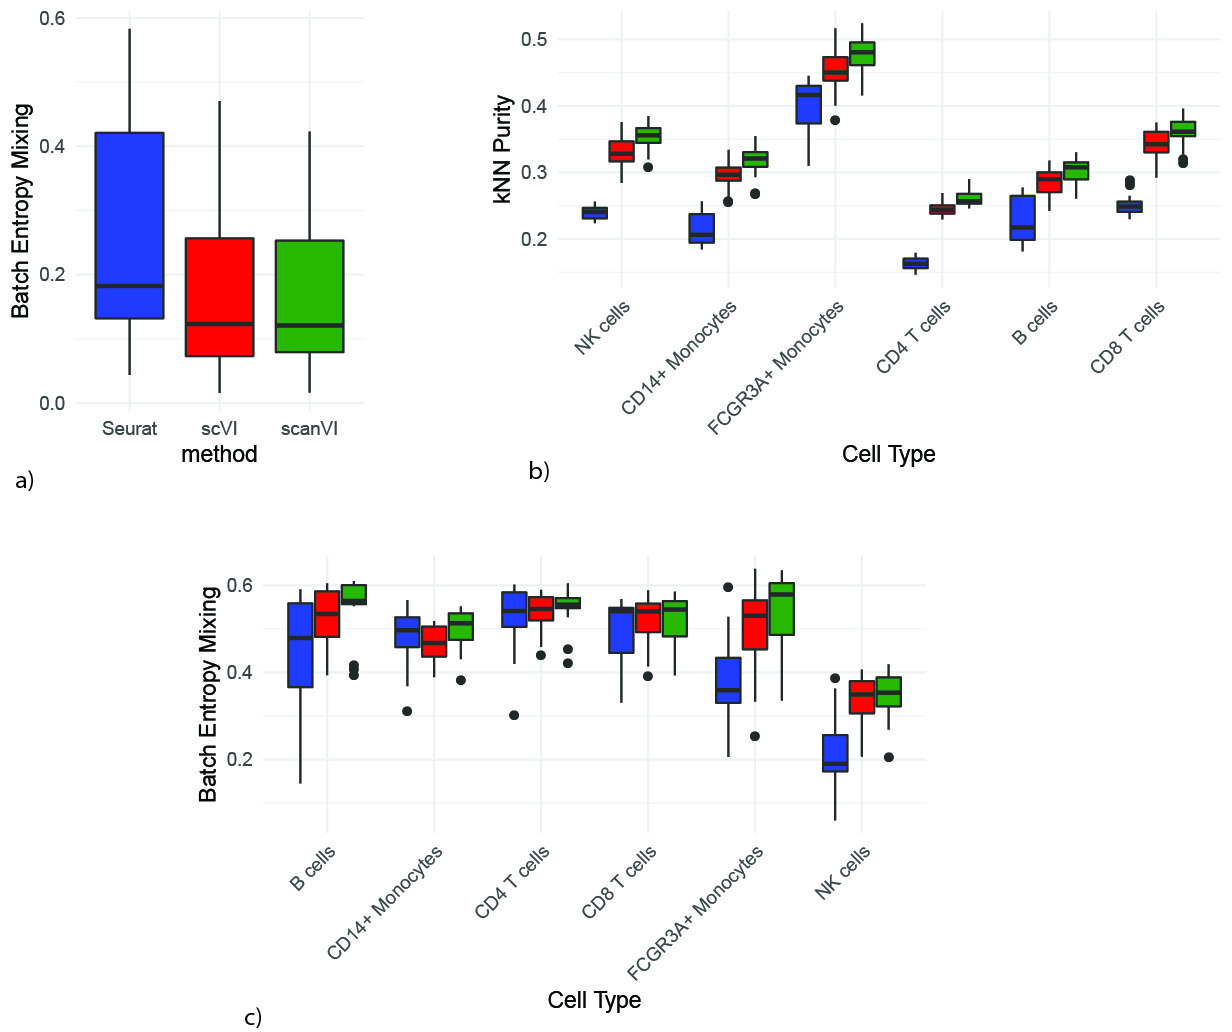
\includegraphics[width=\textwidth]{figures/unique_pops.jpg}
    \caption[Supplementary study of harmonizing datasets with different cellular composition]{Supplementary study of harmonizing datasets with different cellular composition. We show here the case where each of the two datasets has a unique cell types and share all the others. For each box plot, we report over all the possible combinations of left-out cell types. (a) Entropy of batch mixing for the unique population (lower is better). (b) $k$-nearest neighbor purity (unique and non-unique; higher is better). (c) Entropy of batch mixing for the non-unique populations (higher is better). The boxplots are standard Tukey boxplots where the box is delineated by the first and third quartile and the whisker lines are the first and third quartile plus minus 1.5 times the box height. The dots are outliers that fall above or below the whisker lines.}
    \label{scanviunique_pops}
\end{suppfigure}

\begin{suppfigure}[H]
\centering
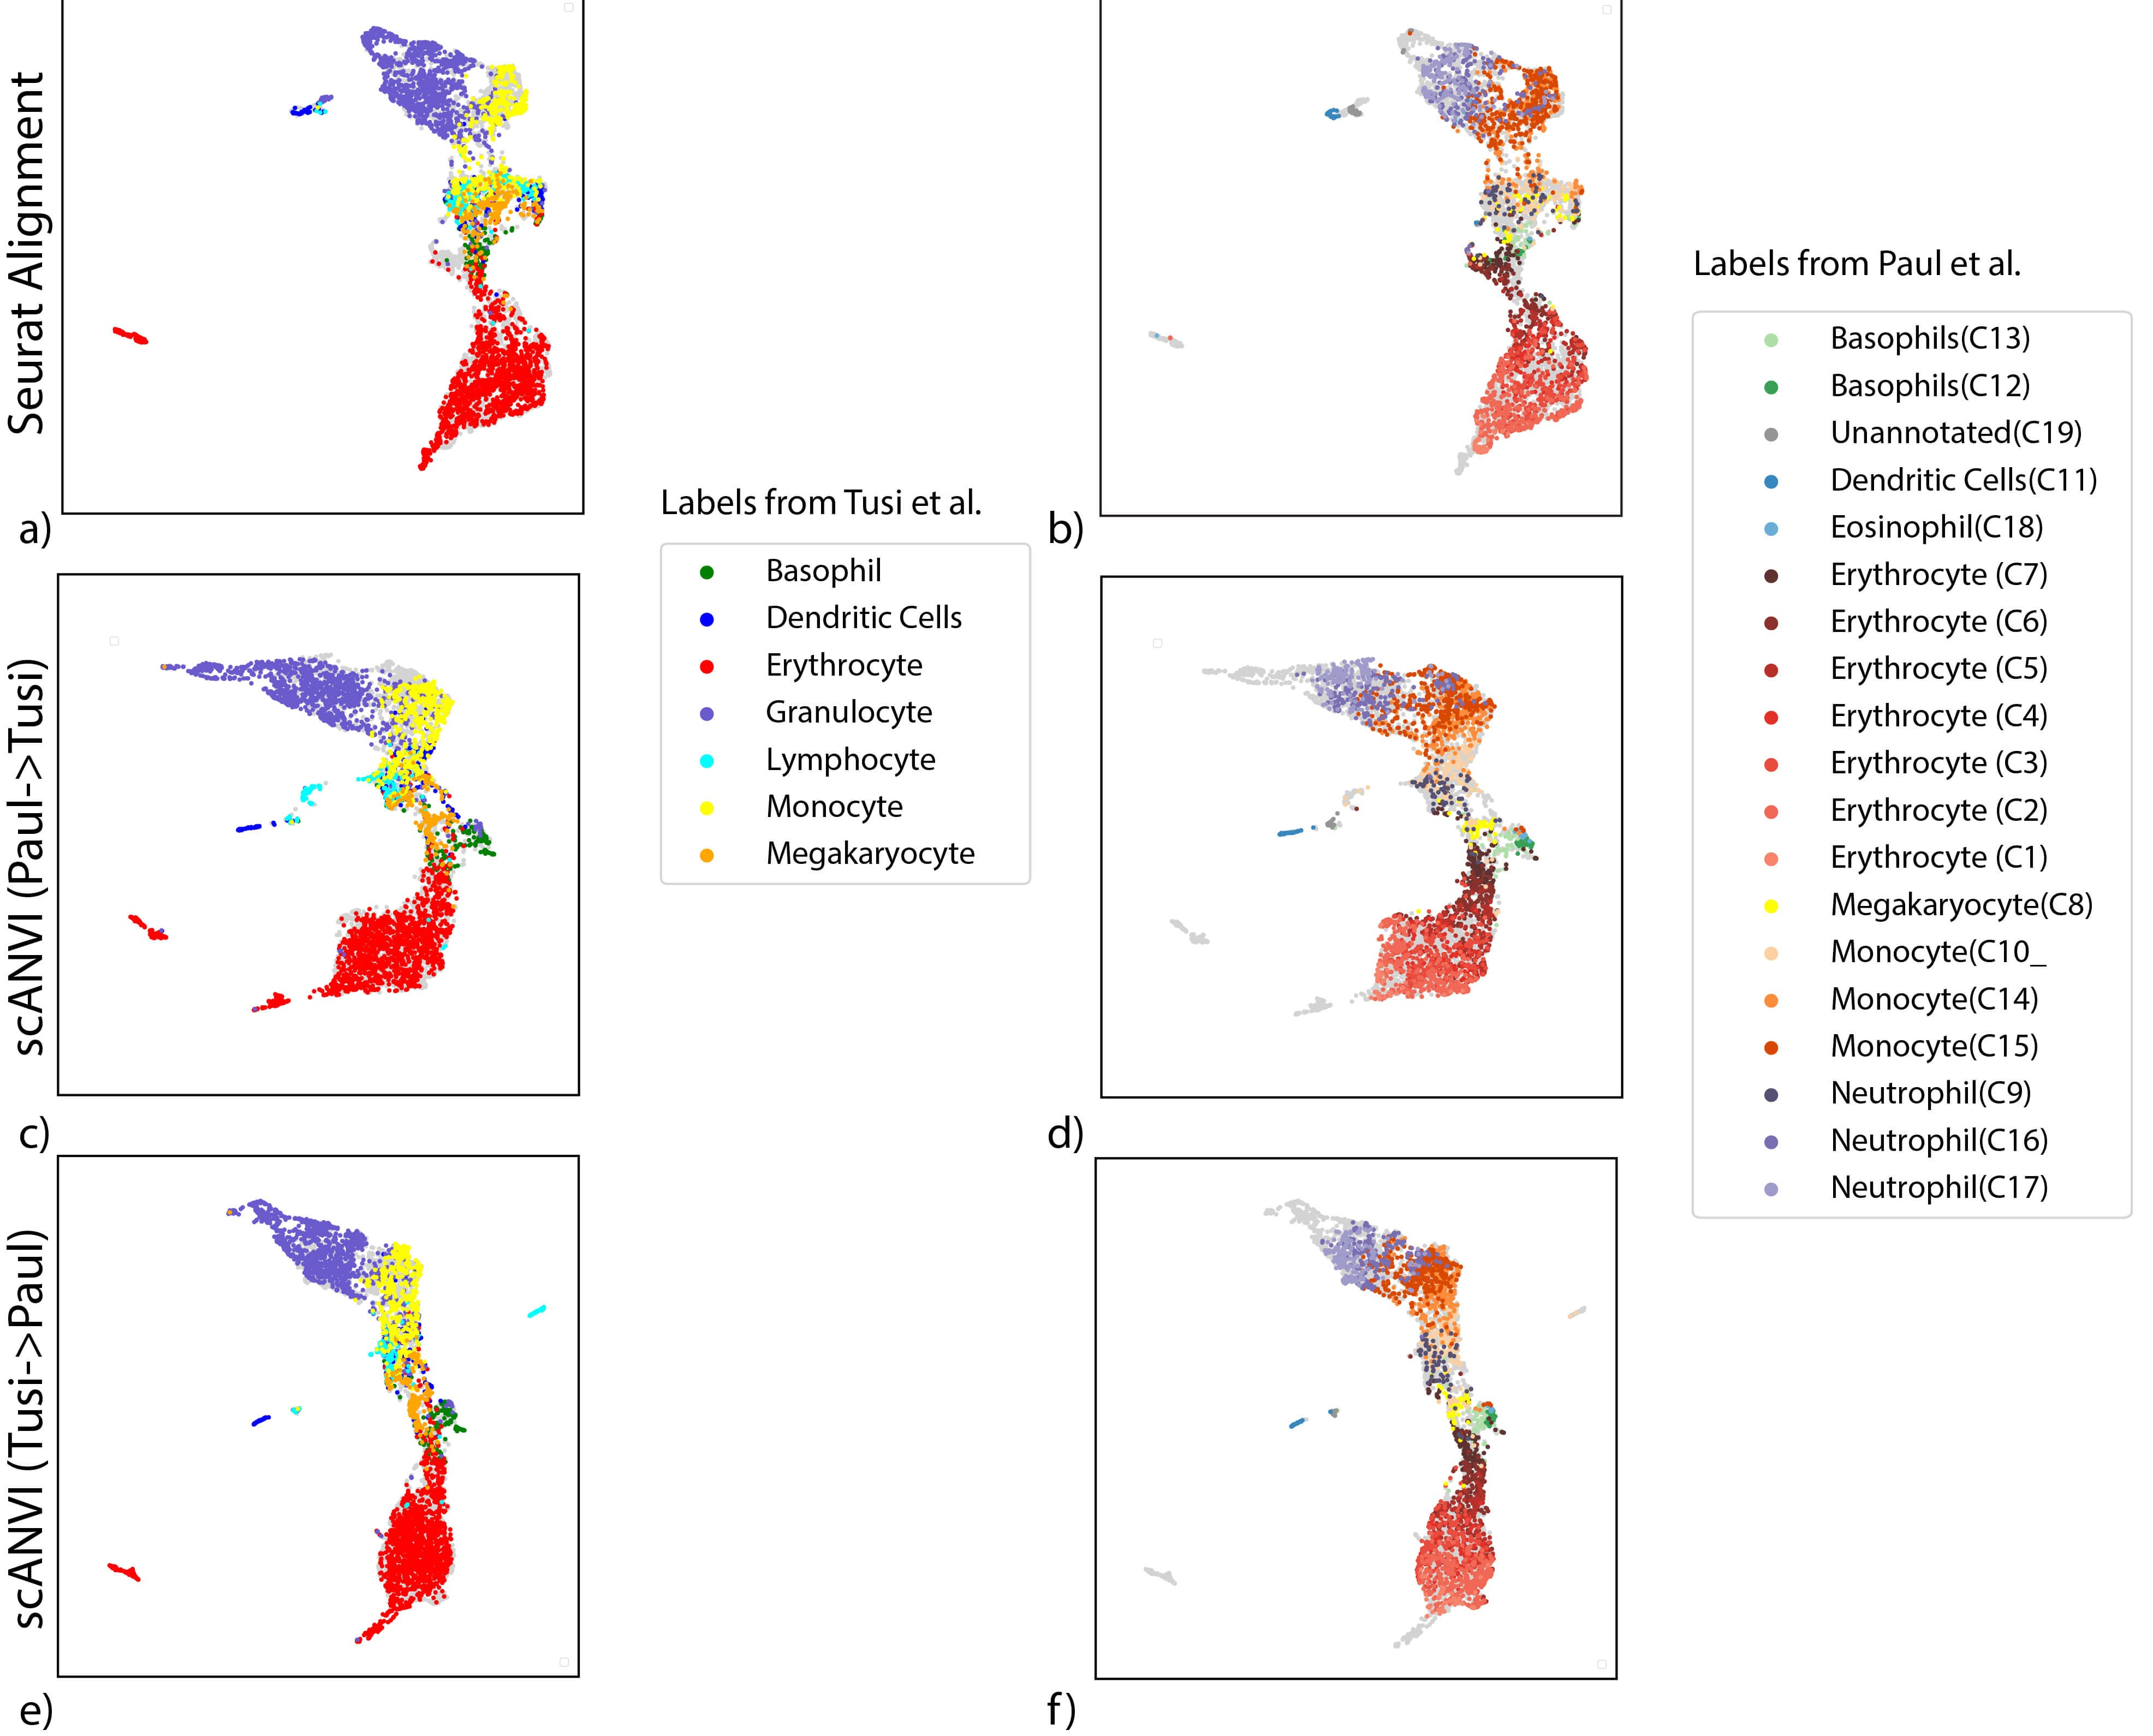
\includegraphics[width=\textwidth]{figures/continuous_supp.jpg}
\caption[Follow-up analysis on continuous trajectory harmonization with scANVI]{Follow-up analysis on continuous trajectory harmonization with scANVI. $(a-b)$ Continuous trajectory obtained by the Seurat Alignment procedure for the HEMATO-Tusi and the HEMATO-Paul datasets. $(c-d)$ Continuous trajectory obtained by the scANVI using the Tusi cell type labels for semi-supervision. $(e-f)$ Continuous trajectory obtained by the scANVI using the Paul cluster labels for semi-supervision.  All locations for scatter plots are computed via UMAP in their respective latent space. }
\label{scanvicontinuousSupp}
\end{suppfigure}


\begin{suppfigure}[H]
\centering
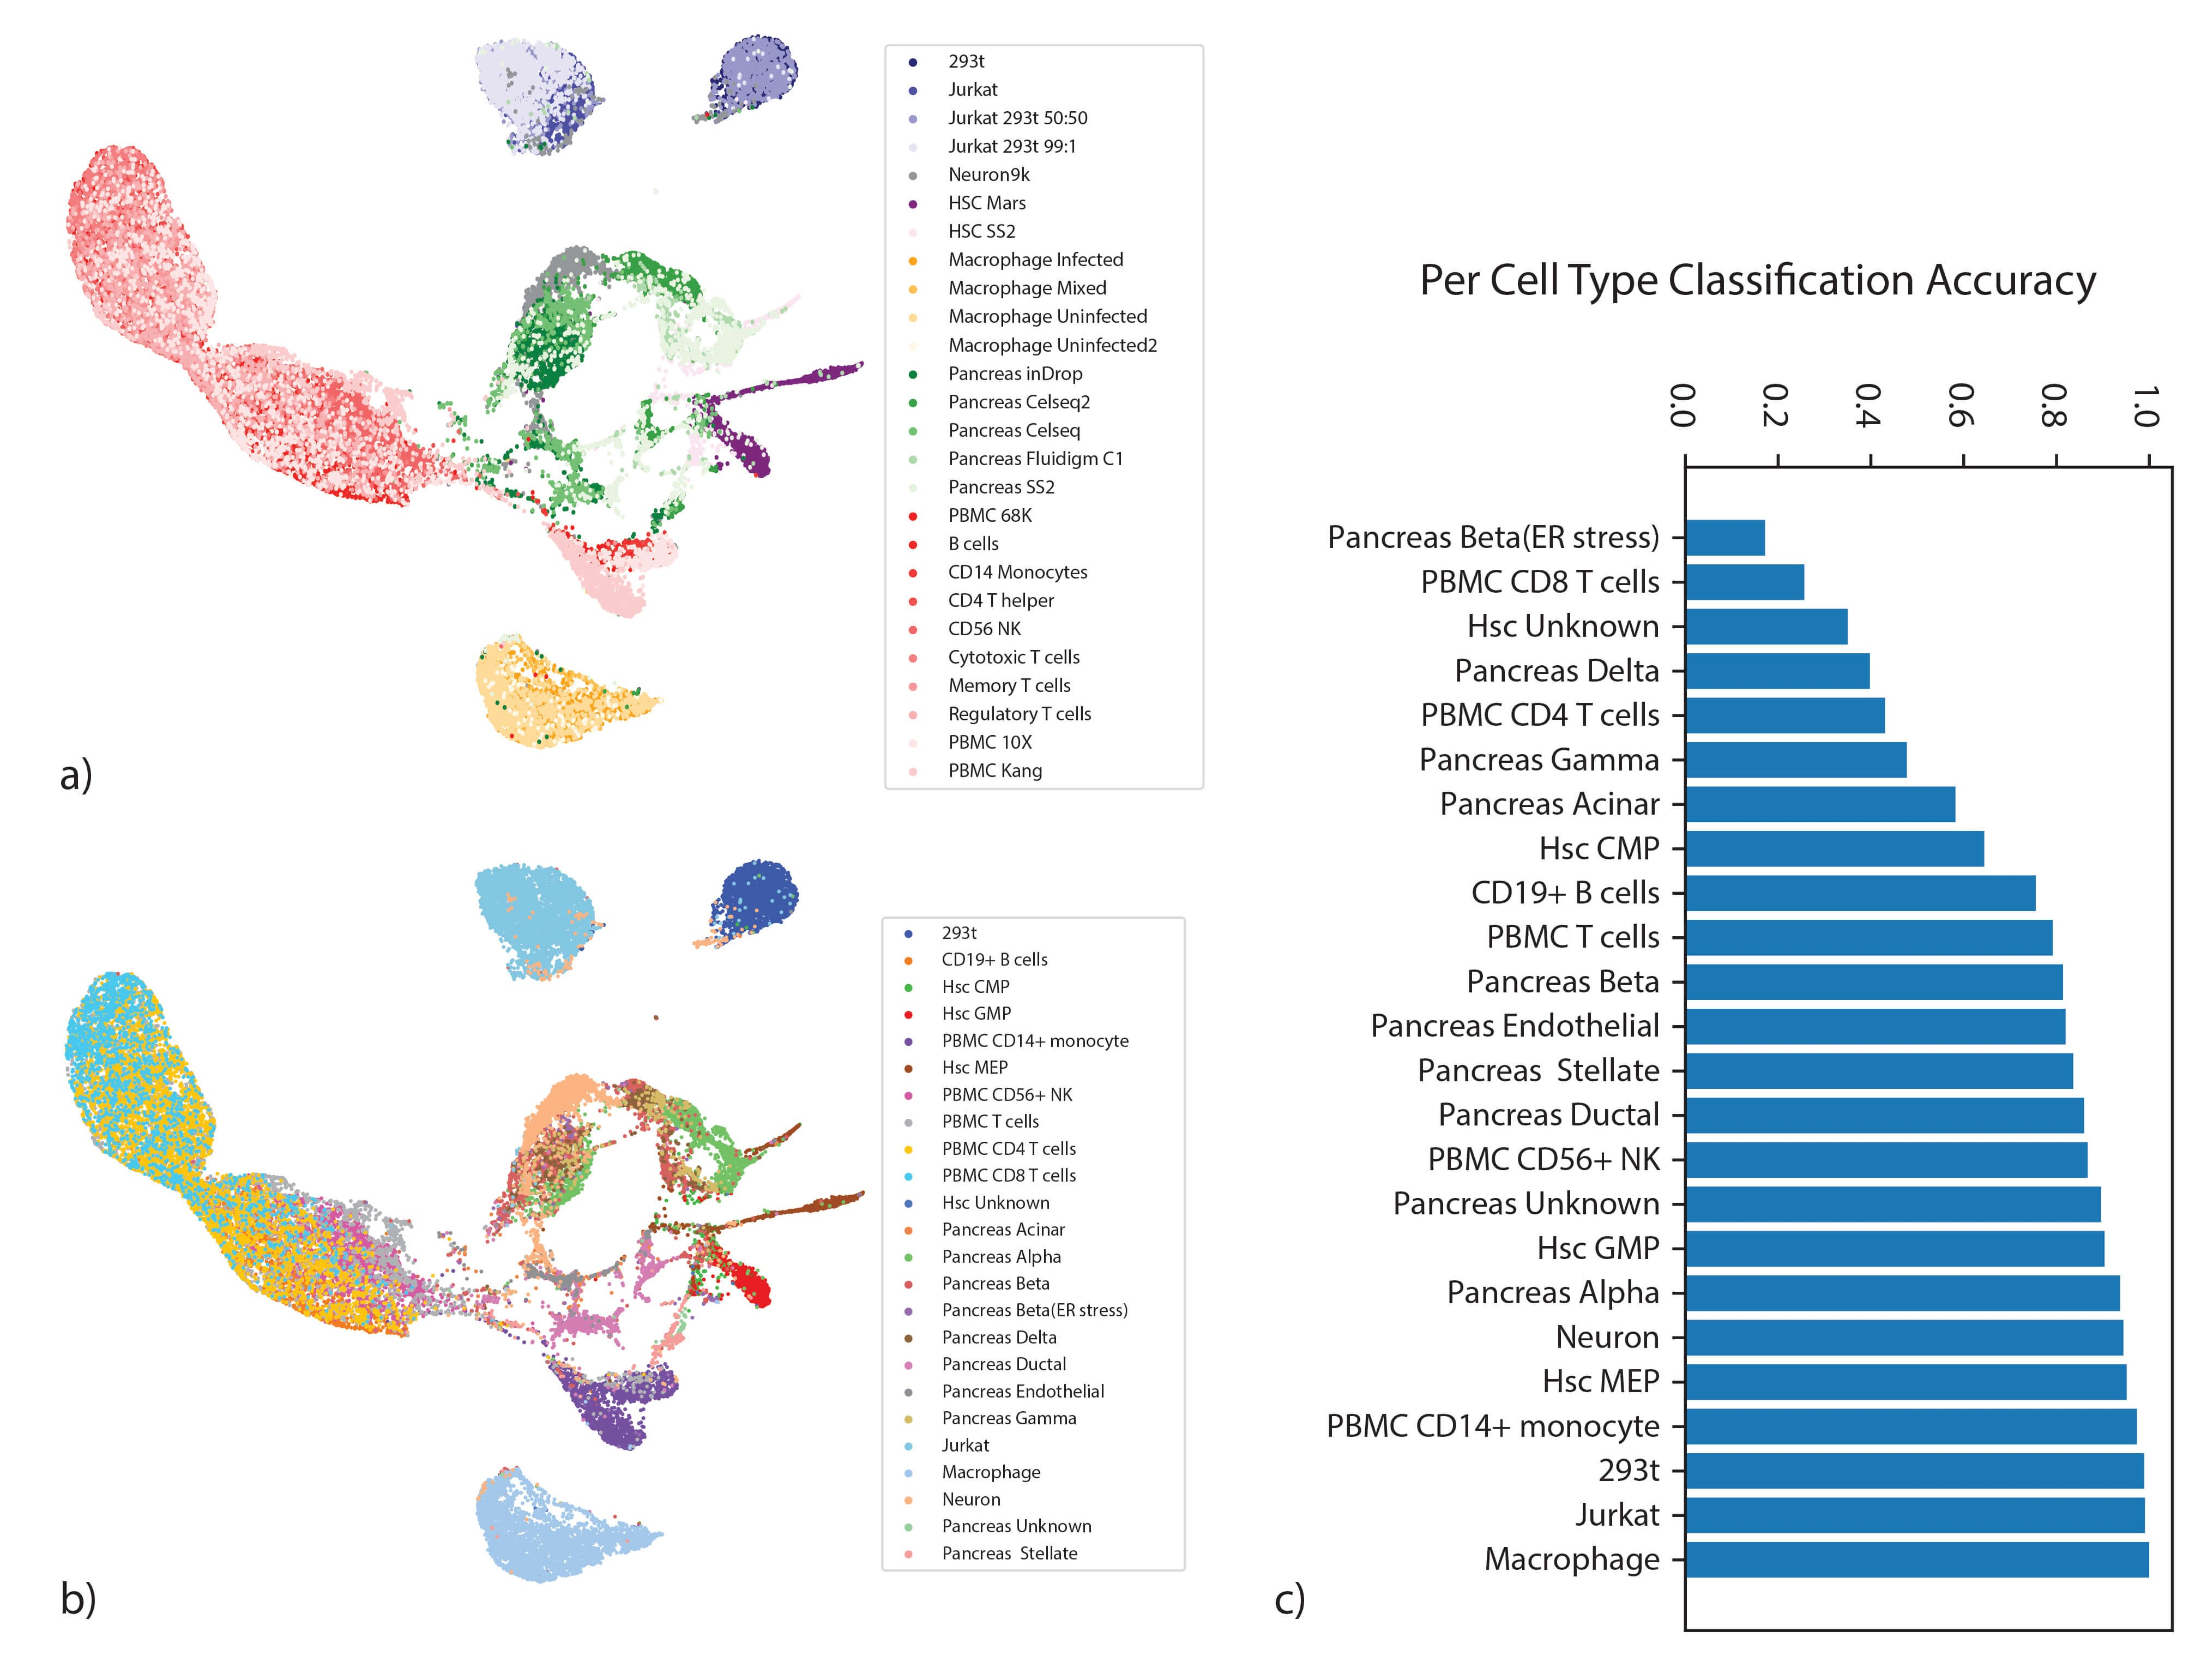
\includegraphics[width=\textwidth]{figures/scanorama.jpg}
\caption[Large-scale data integration with scVI]{Large-scale data integration with scVI. $(a-b)$ UMAP visualization of the scVI latent space colored by datasets $(a)$ and by cell types $(b)$. $(c)$ accuracy of a nearest neighbor classifier based on scVI latent space}
\label{scanvilarge_scale_panel}
\end{suppfigure}

\begin{suppfigure}[H]
\centering
\includegraphics[width=0.7\textwidth]{figures/acc_boxplot.jpg}
\caption[Annotation results for all four dataset pairs (boxplot)]{Annotation results for all four dataset pairs. PBMC-8K / PBMC-cite $(a-b)$, MarrowMT-10X / MarrowMT-SS2 $(c-d)$, Pancreas InDrop-CELSeq2 $(e-f)$ and Dentate Gyrus 10X / Fluidigm C1 $(g-h)$. Accuracies for transferring annotations from one dataset to another from a $k$-nearest neighbors classifier on Seurat Alignment, and scVI latent space, scANVI, SCMAP and CORAL classifier are shown.  The aggregated results across for cell types that are shared between the two datasets is shown in box plots.  }
\label{scanviaccbox}
\end{suppfigure}

\begin{suppfigure}[H]
\centering
\includegraphics[width=0.9\textwidth]{figures/bubbles.jpg}
\caption[Annotation results for all four dataset pairs (bubbleplot)]{Annotation results for all four dataset pairs. PBMC-8K / PBMC-cite $(a-b)$, MarrowMT-10X / MarrowMT-SS2 $(c-d)$, Pancreas InDrop-CELSeq2 $(e-f)$ and Dentate Gyrus 10X / Fluidigm C1 $(g-h)$.  Accuracies for transferring annotations from one dataset to another from a $k$-nearest neighbors classifier on Seurat Alignment, and scVI latent space, scANVI, SCMAP and CORAL classifier are shown.  The prediction accuracy  for each cell type that is shared between the two datasets is shown on the y-axis and the size of the dots are proportional to the proportion of a cell type in the total population. }
\label{scanvibubble}
\end{suppfigure}


\begin{suppfigure}[H]
\centering
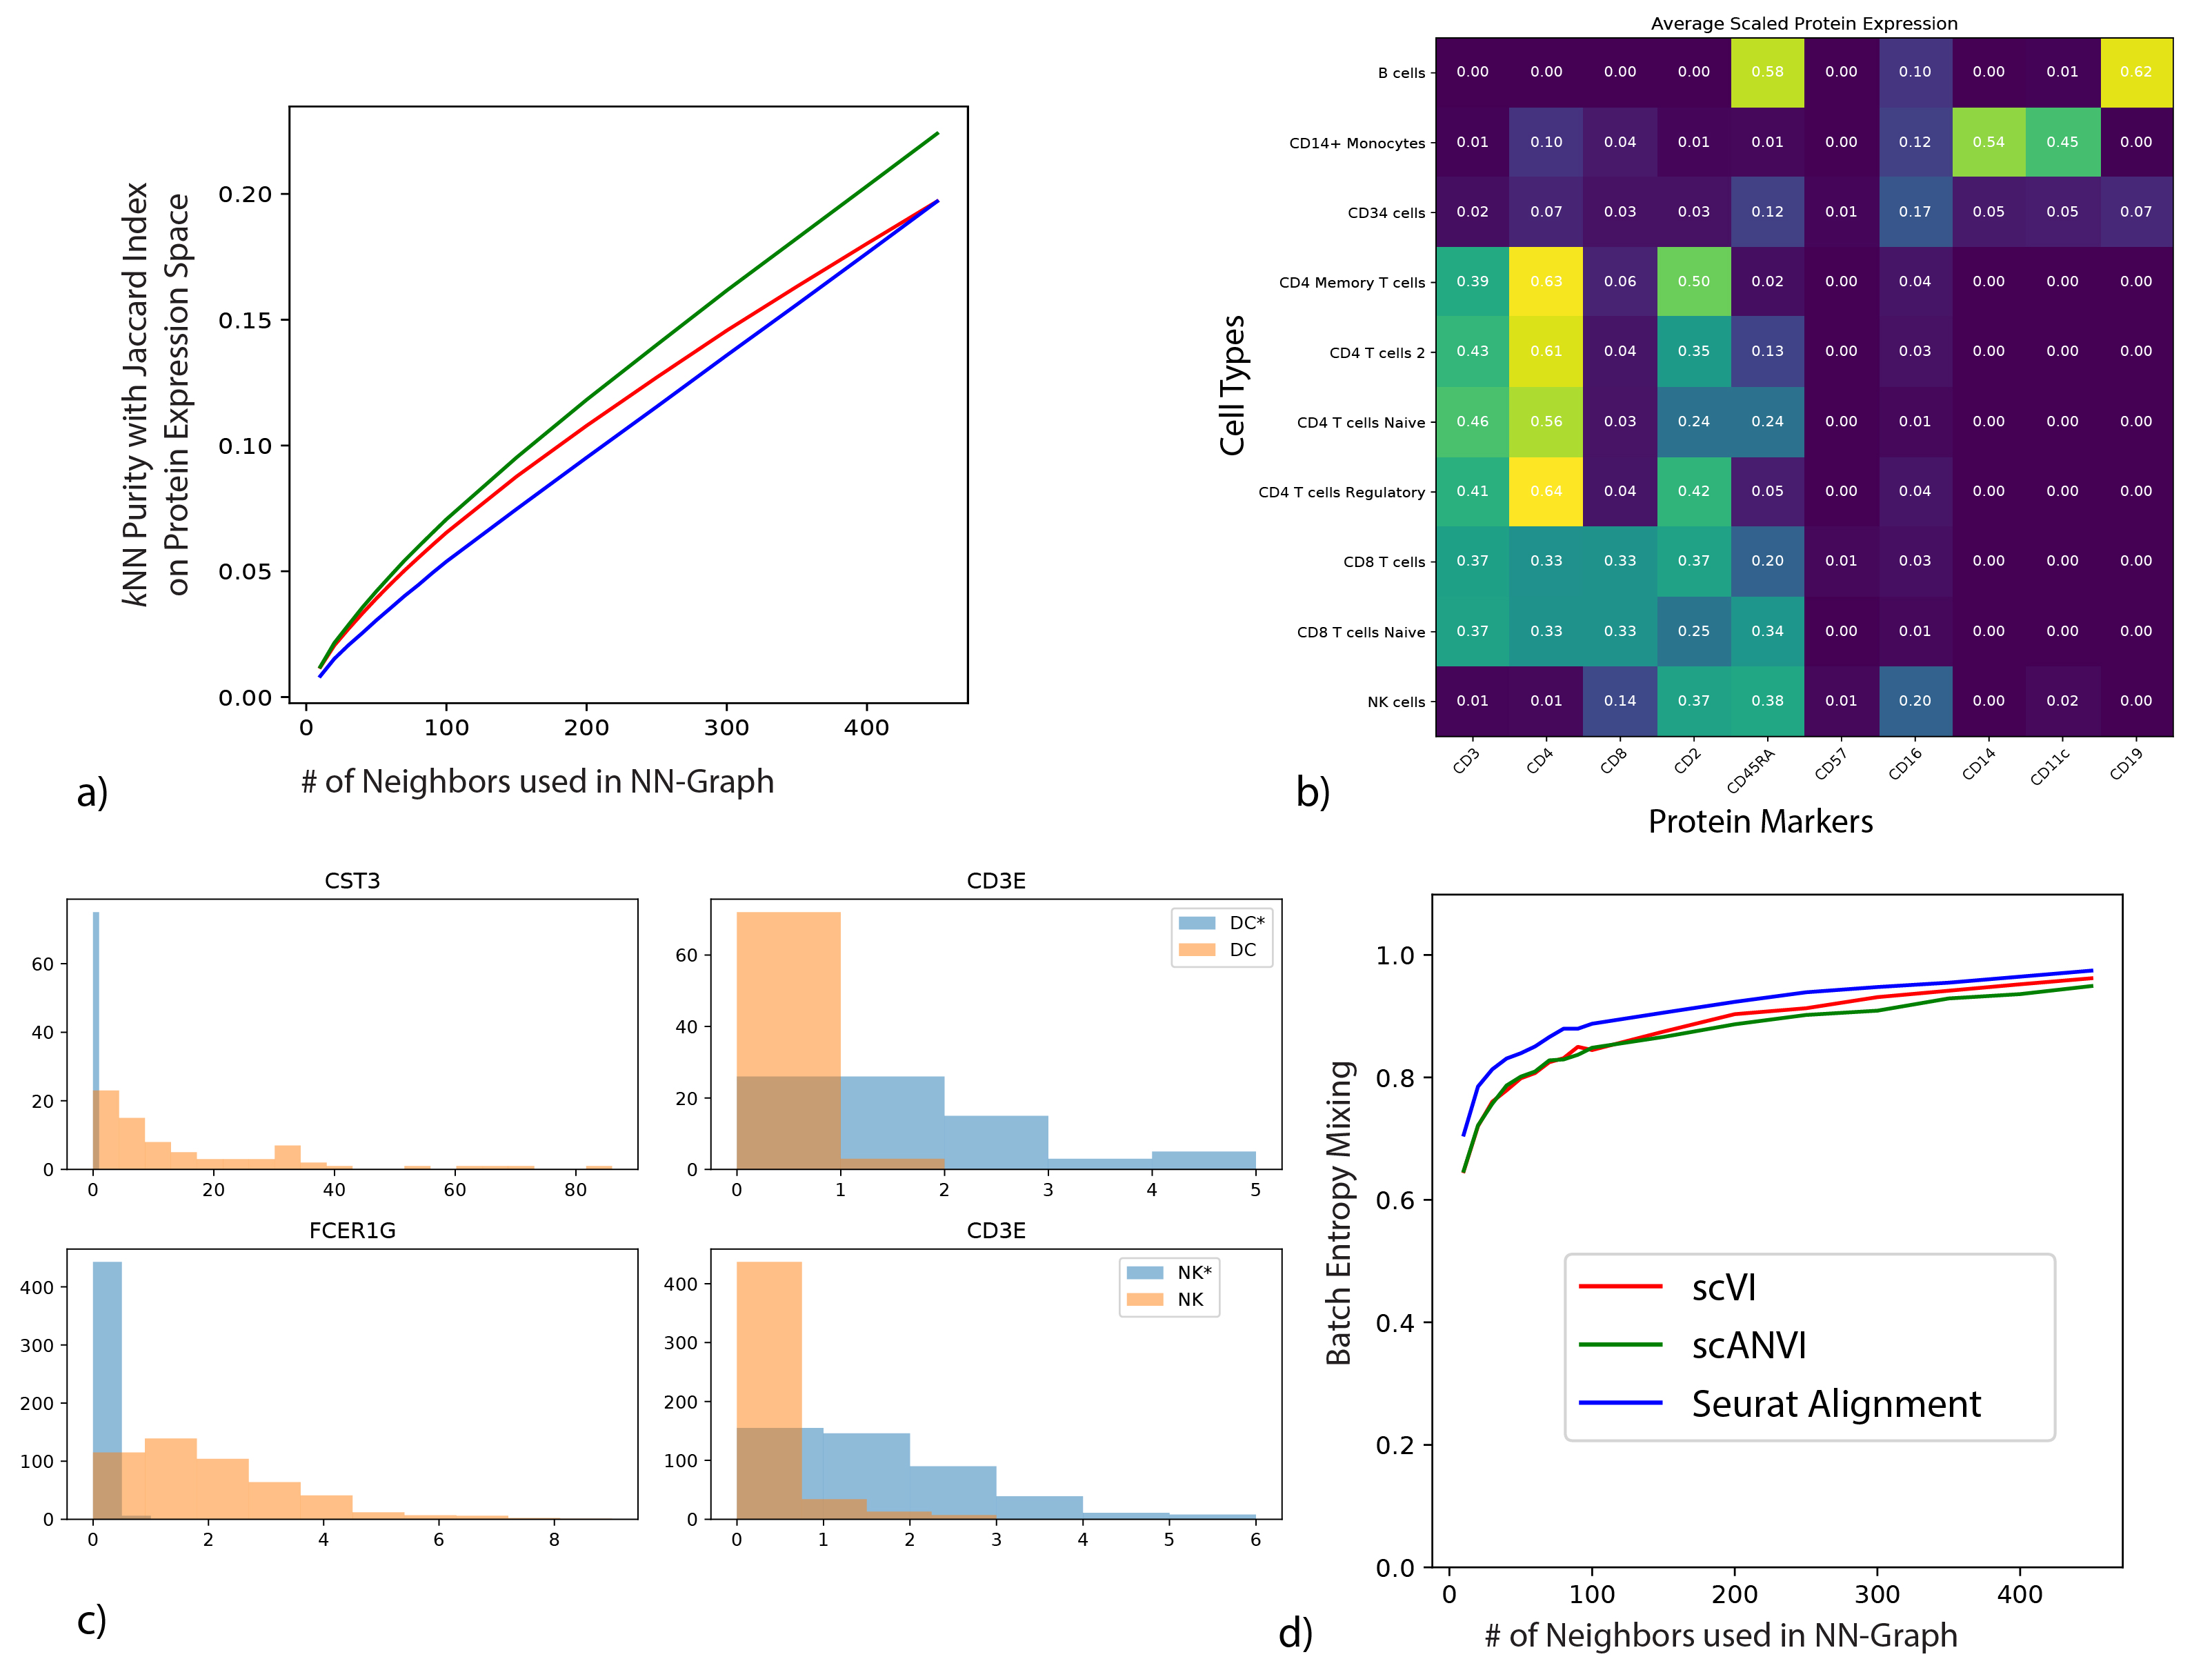
\includegraphics[width=\textwidth]{figures/labels_concored_supp.jpg}
\caption[Supplementary study of labels concordance]{Supplementary study of labels concordance. $(a)$ $k$-nearest neighbors purity of the merged latent space on the protein expression space as a function of the size of the neighborhood. $(b)$ Protein expression heatmap showing consistency of PBMC-Sorted labels and protein expression in PBMC-CITE. The protein expression per cell type is based on $k$-nearest neighbors imputation from the harmonized latent space obtained from scANVI trained with pure population labels. $(c)$ We select individual cells that were  labeled as dendritic cells or Natural Killer cells in the original publication of the respective datasets, and compare the raw transcript count from cells inside the scANVI T cells cluster (DC*, NK*) against cells outside the T cells cluster (DC, NK). The expression of marker genes suggest that DC* and NK* is more likely to be T cells and thus the scANVI latent space is more accurate. $(d)$ The batch entropy mixing of the three datasets in scVI, scANVI and Seurat Alignment merged space. }
\label{scanviconcord_supplement}
\end{suppfigure}




\begin{suppfigure}[H]
\centering
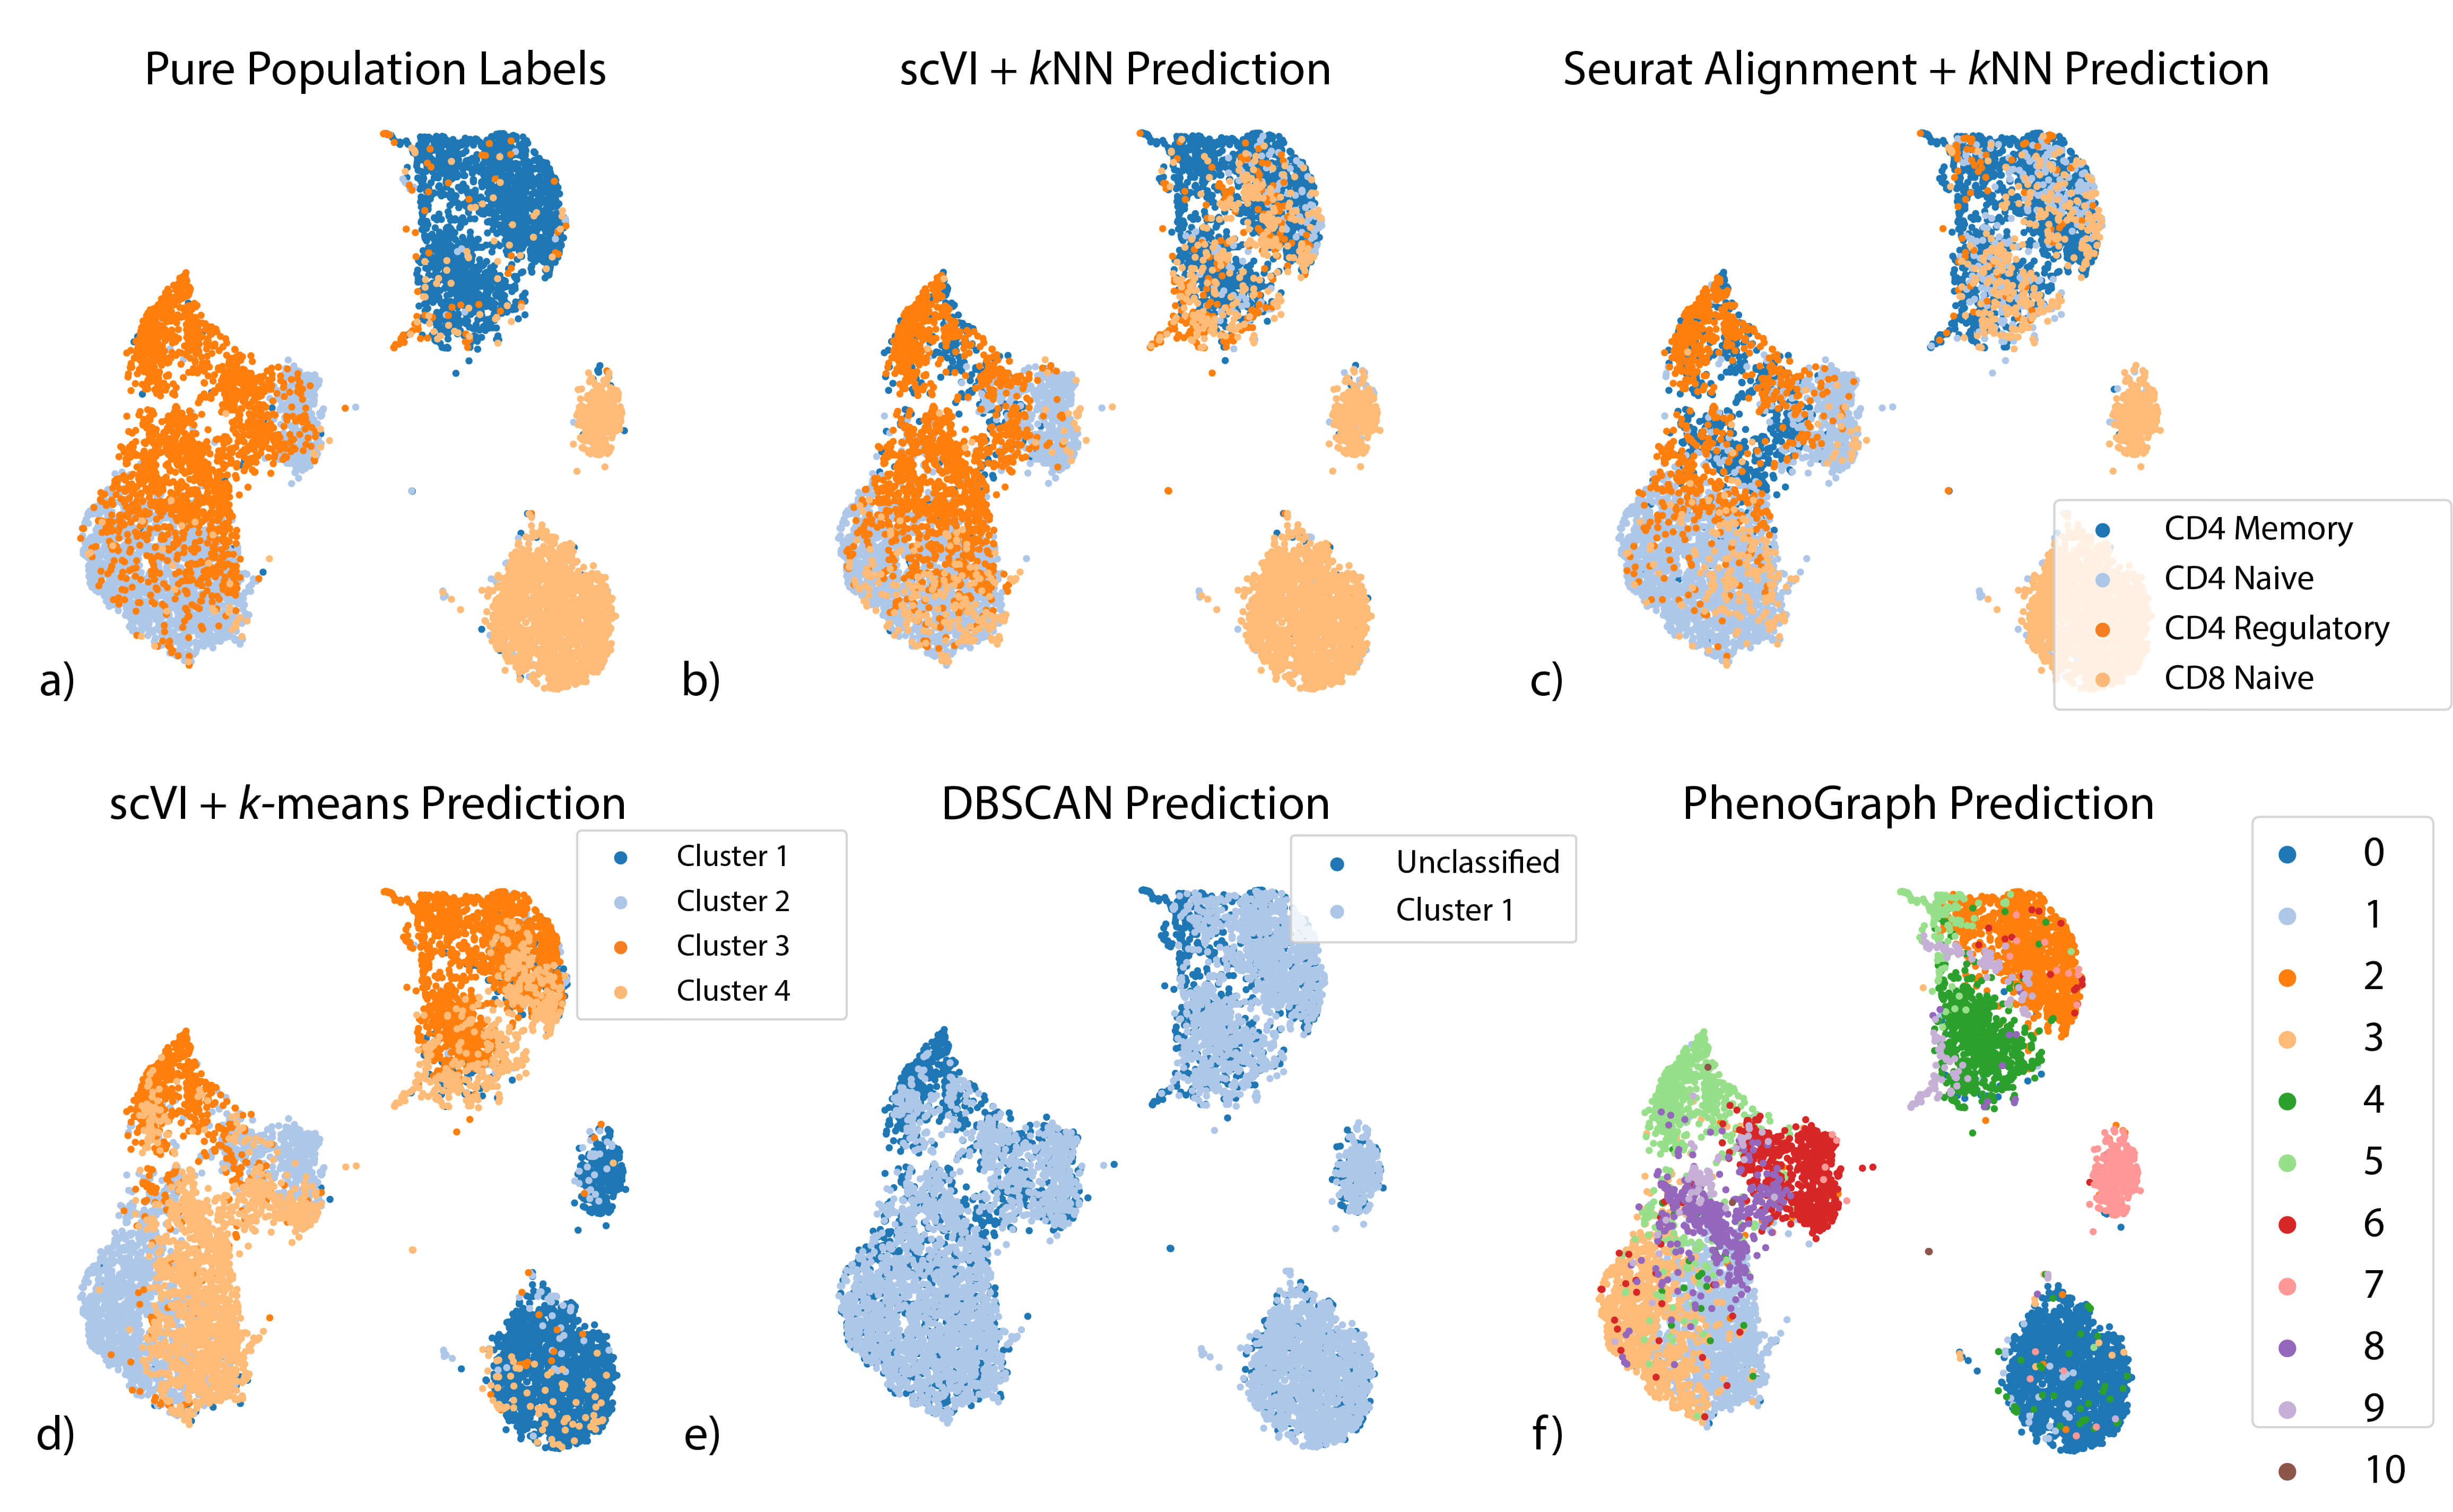
\includegraphics[width=\textwidth]{figures/scanvi_supp.jpg}
\caption[Other methods of classifying T-cell subsets of the PBMC-Pure dataset]{Other methods of classifying T-cell subsets of the PBMC-Pure dataset. Coordinates for the scatter plots are derived from UMAP embedding based on the latent space of scANVI. $(a)$ Ground truth labels from the purified PBMC populations $(b)$ $k$-nearest neighbors classification labels when applied on scVI latent space from the seed set of cells $(c)$ $k$-nearest neighbors classification labels when applied on Seurat Alignment latent space $(d)$ $k$-means clustering based labels when applied to scVI latent space $(e)$ DBSCAN clustering based labels when applied to scVI latent space. DBSCAN returns only one cluster but return some cells as unclassified. $(f)$ PhenoGraph clusters on scVI latent space}
\label{scanviscanviClustering}
\end{suppfigure}

\begin{suppfigure}[H]
    \centering
    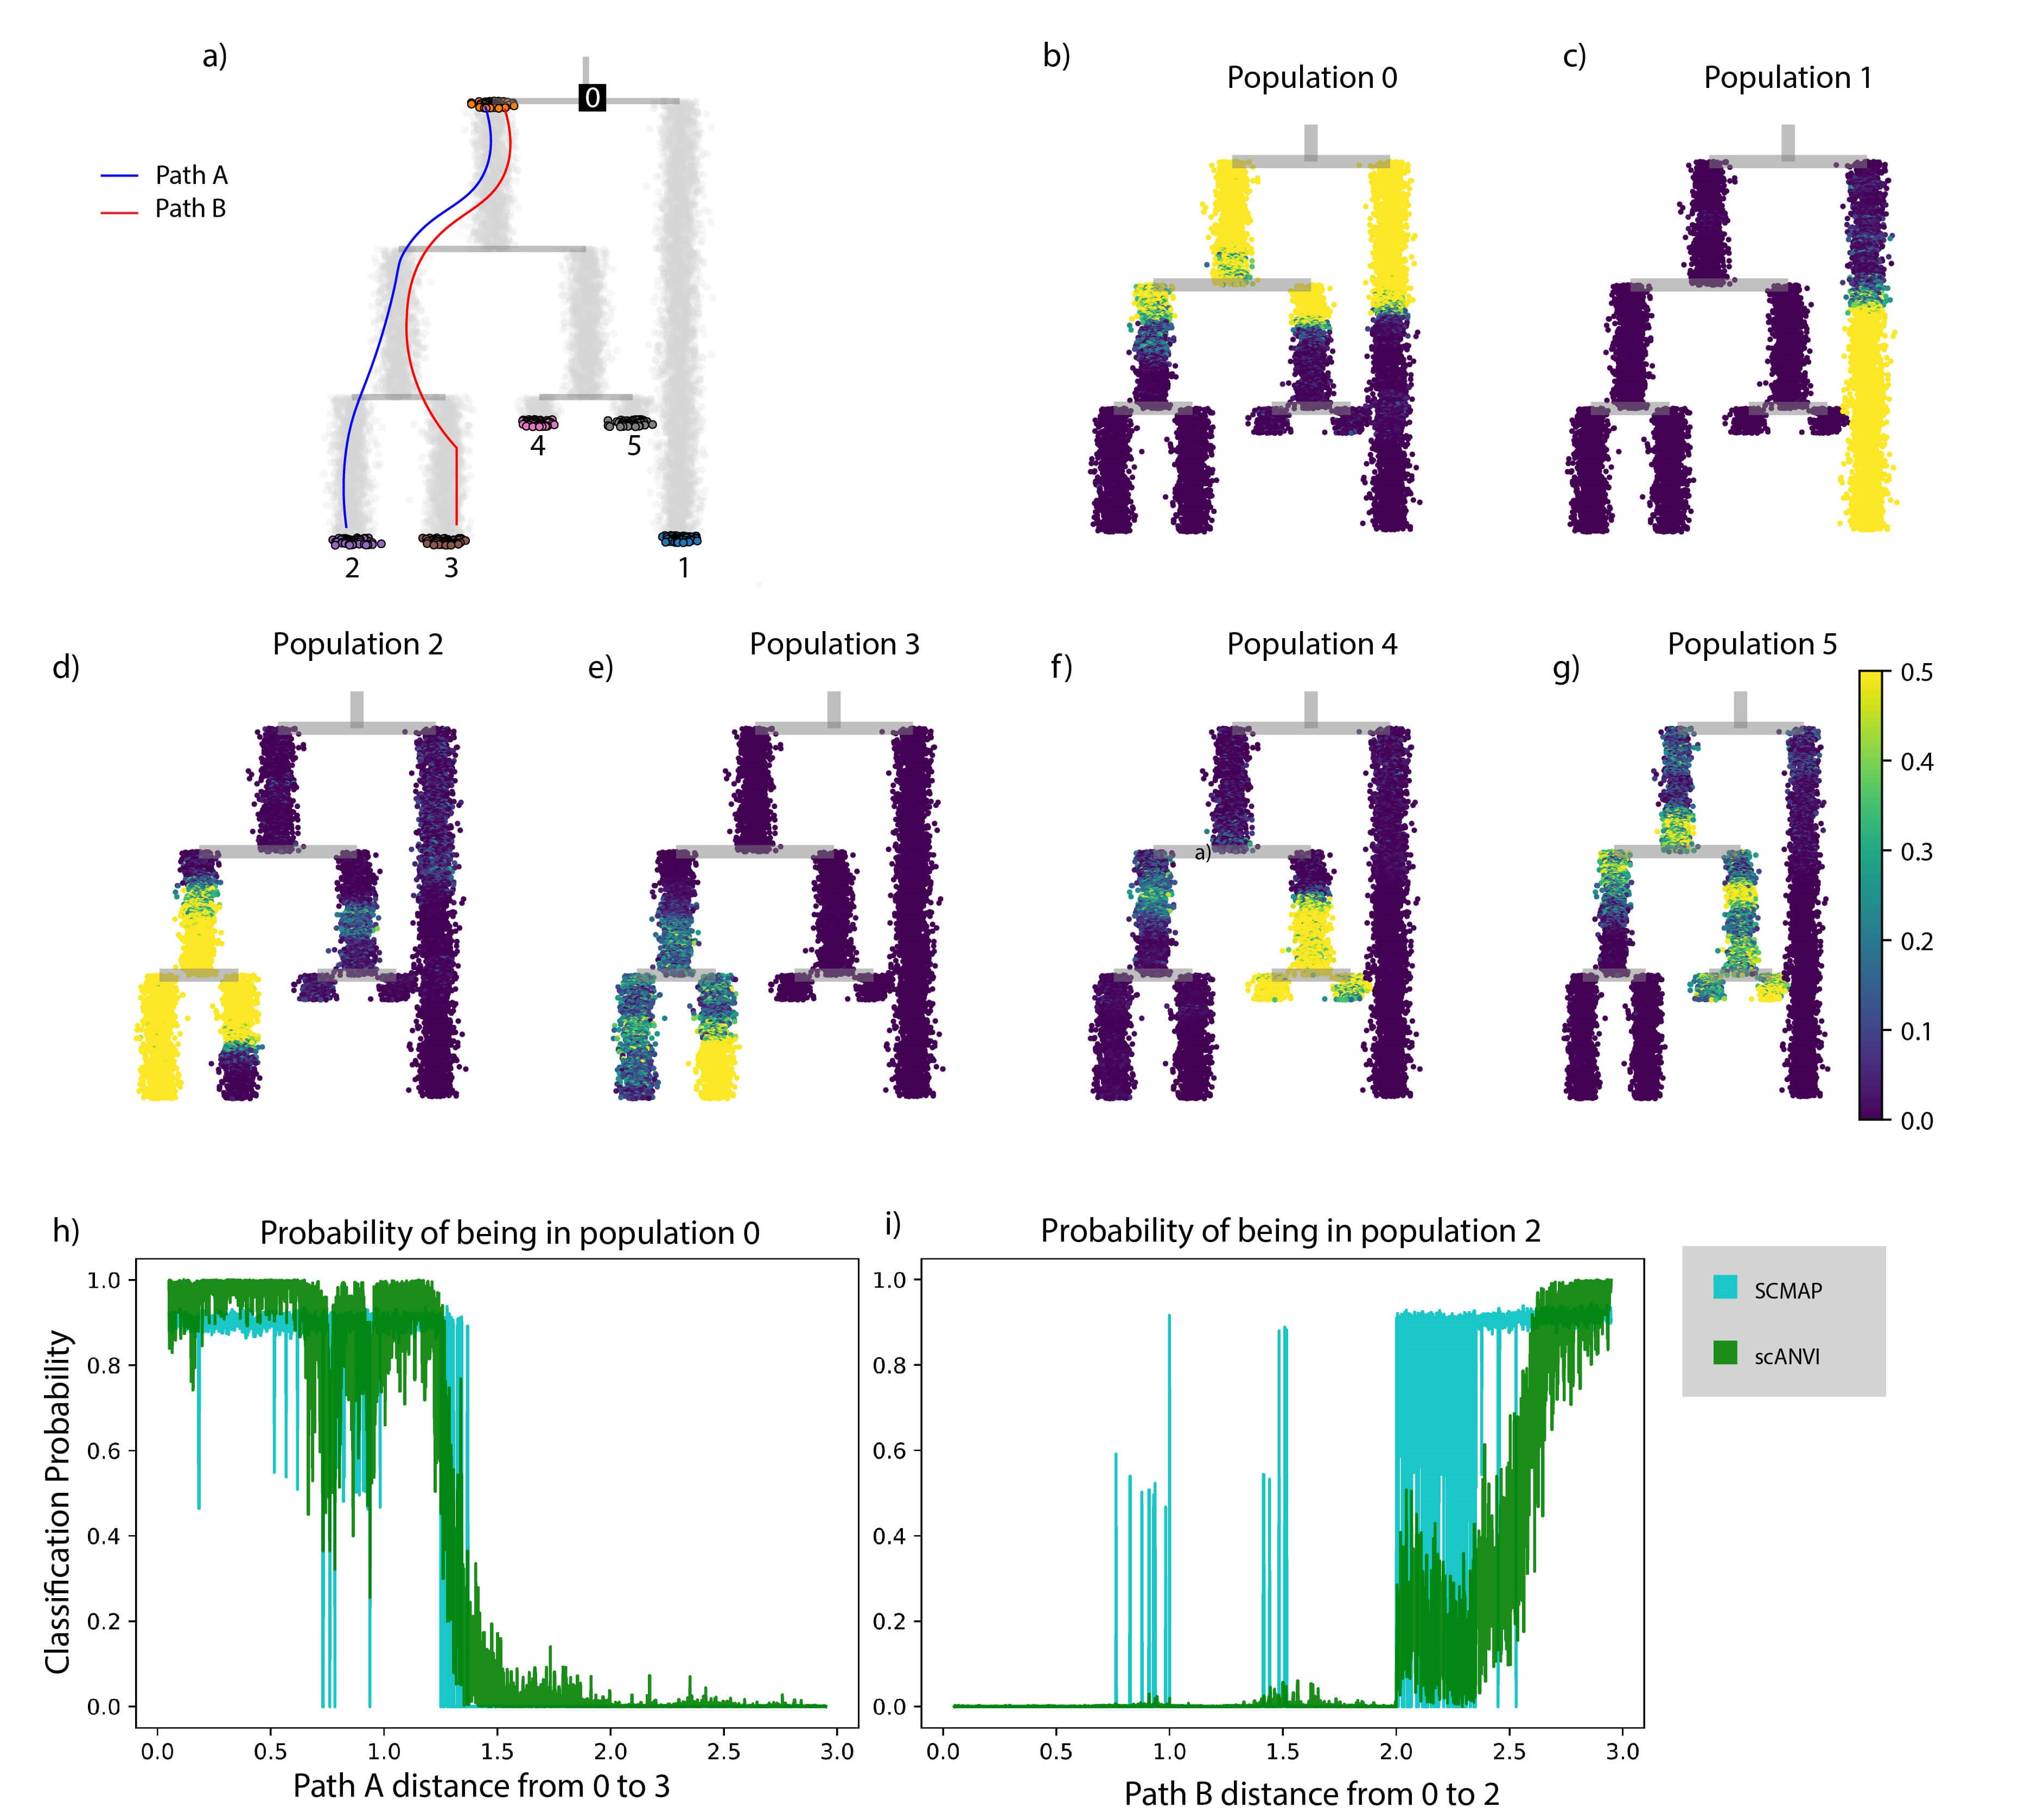
\includegraphics[width=\textwidth]{figures/symsim_continuous.jpg}
    \caption[Continuous trajectory simulated using SymSim]{Continuous trajectory simulated using SymSim. $(a)$ Tree structure from which the cells are sampled. Each grey dot represent a cell sampled along the trajectory. Colored dots with a black edge are treated as labeled, while the others are treated as unlabeled. Each path simulates a continuous phenotypical variation. $(b-g)$ The same tree with each cell colored by the posterior probability of being assigned to a specific label. $(h-i)$ Another visualization of the gradual change of posterior probability by plotting the posterior probability of root $(h)$ and population 3 $(i)$. The x-axis represents the pathwise distance (paths are defined in $(a)$), and the y-axis represents the probability, or confidence of the assignment.}
    \label{scanvisymsim_cont}
\end{suppfigure}

\begin{suppfigure}[H]
    \centering
    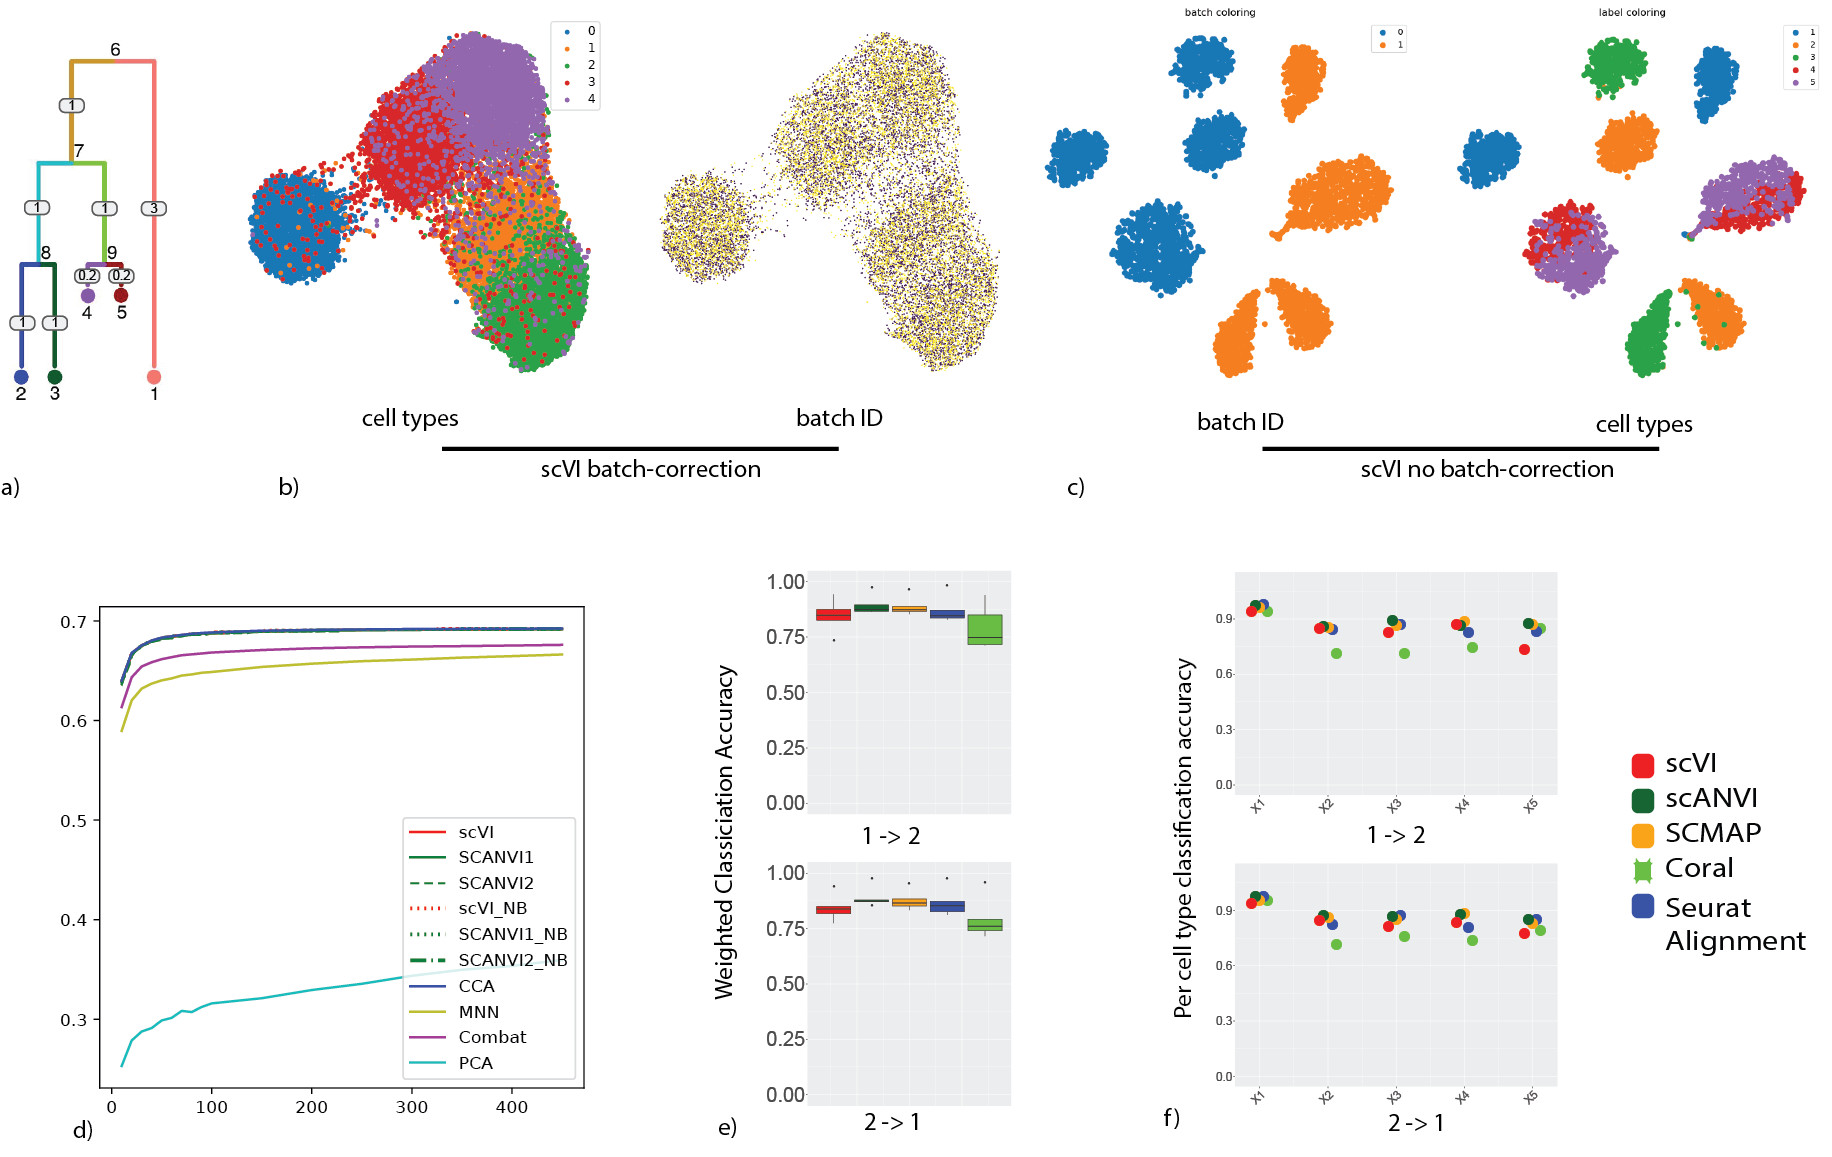
\includegraphics[width=\textwidth]{figures/panel_simulations.png}
    \caption[Presentation of the simulated dataset used for differential expression benchmarking]{Presentation of the simulated dataset used for differential expression benchmarking. (a) The tree used to sample the cells in SymSim. We sample cells from the five leaves nodes representing five different cell types derived from the same root node. (b) UMAP of scVI latent space colored by cell types and batch identifier (c) UMAP of scVI latent space without batch correction, proving that the data is indeed subject to batch effects. (d) Entropy of batch mixing for all the algorithms (e) Weighted accuracy using a $k$-nearest neighbors classifier on the latent space (f) Per cell type accuracy for the label transfer. }
    \label{scanvisimulations_panel}
\end{suppfigure}

\begin{suppfigure}[H]
\centering
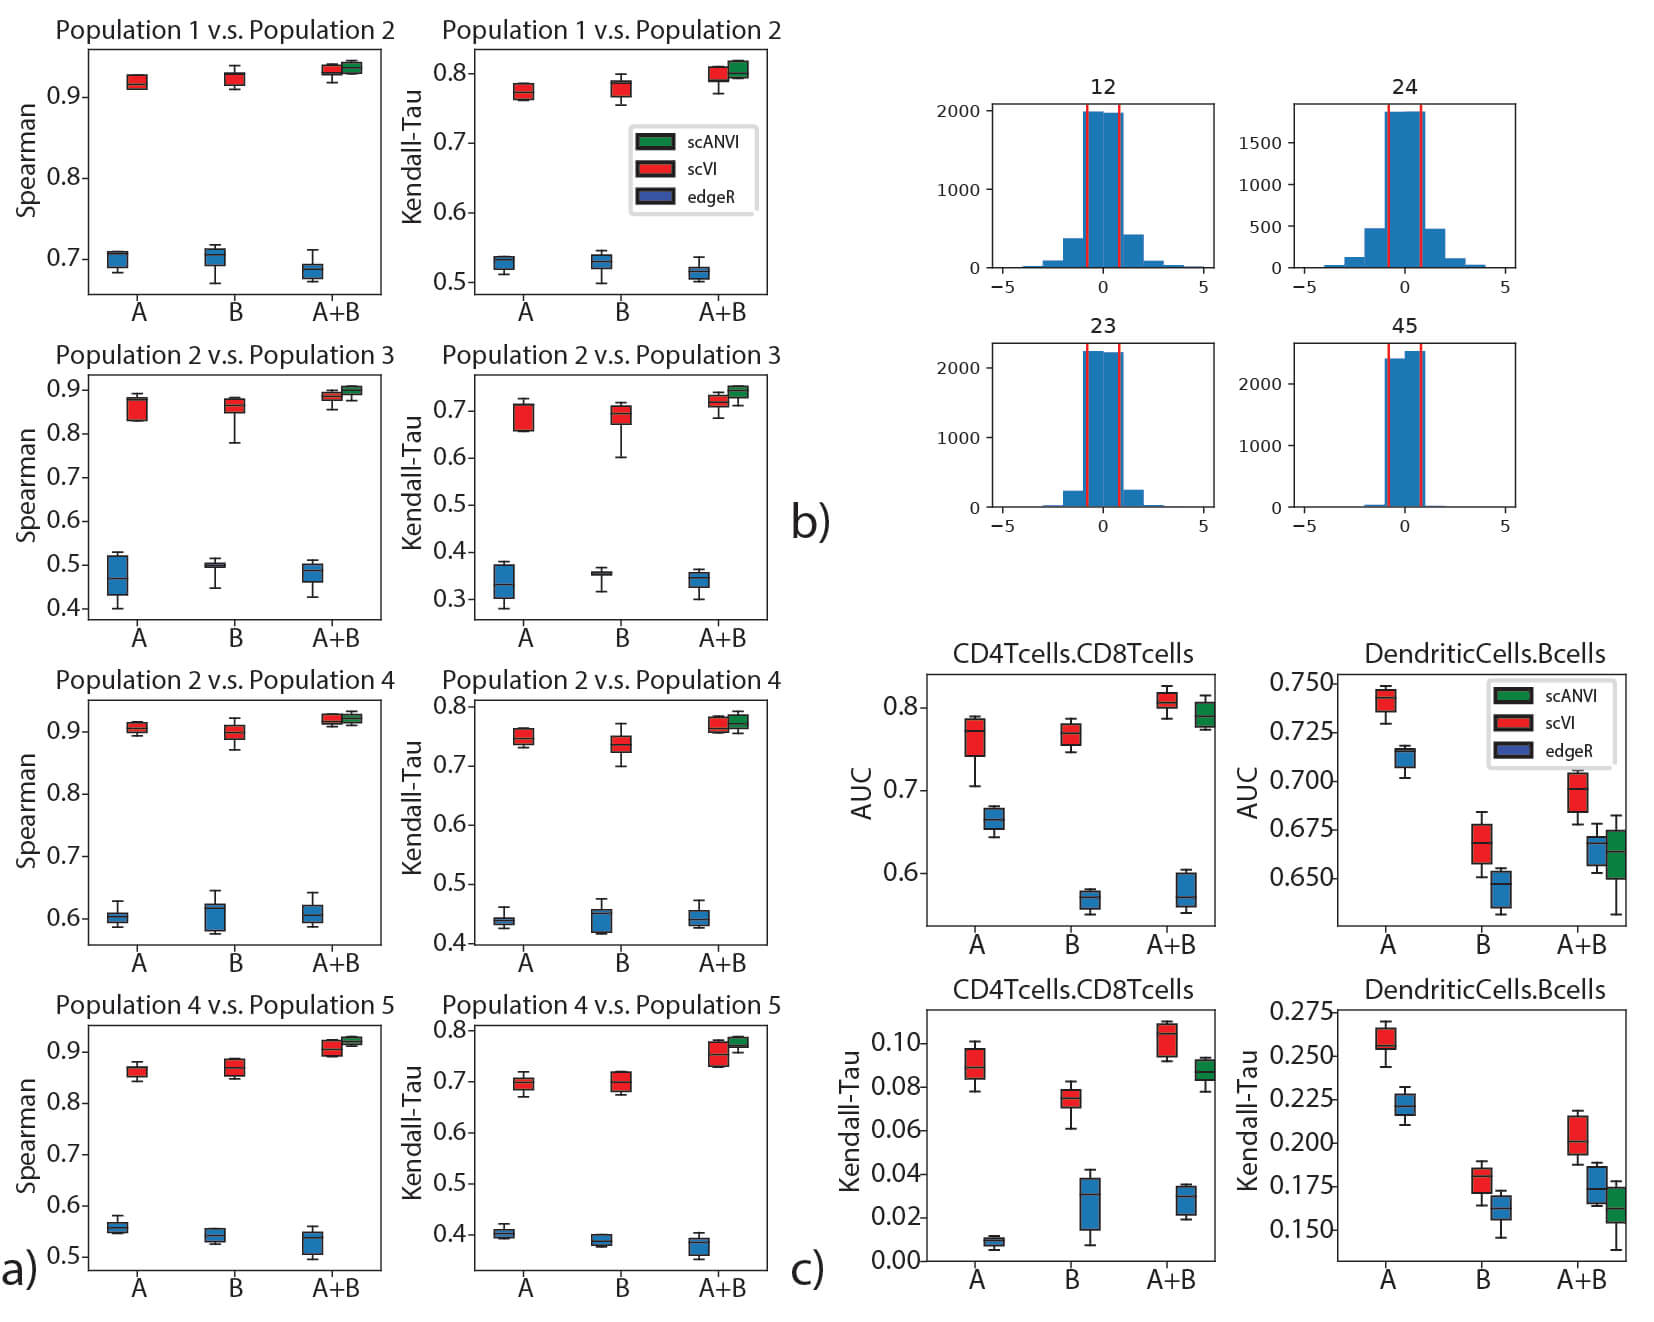
\includegraphics[width=\textwidth]{figures/de_new.jpg}
\caption[Differential Expression on multiple datasets with scVI]{Differential Expression on multiple datasets with scVI. $(a)$ Evaluation of consistency with rank correlation is shown for comparisons of multiple pairs of cell types in the simulated data. The pairs of cells are chosen to represent different levels of distance on the tree as in Figure~\ref{scanvisimulations_panel}a. The pairs of population from most distant to least distant are `12', `24', `23', `45'. $(b)$ distribution of true log fold change between all pairs of cell types for the simulated data. $(c)$ Evaluation of
consistency with the AUROC and Kendal Tau metric is shown for comparisons of CD4 vs CD8 T cells and B cells vs dendritic cells on the PBMC-8K only (A), the PBMC-68k only (B) and the merged PBMC-8K / PBMC-68K (A+B) for scVI and edgeR. Error bars are obtained by multiple subsampling
of the data to show robustness. Boxplots are standard Tukey boxplots where the box is delineated by the first and third quartile and the whisker lines are the first and third quartile plus minus 1.5 times the box height. The dots are outliers that fall above or below the whisker lines.}
\label{scanviDE_panel}
\end{suppfigure}

\begin{suppfigure}[H]
\centering
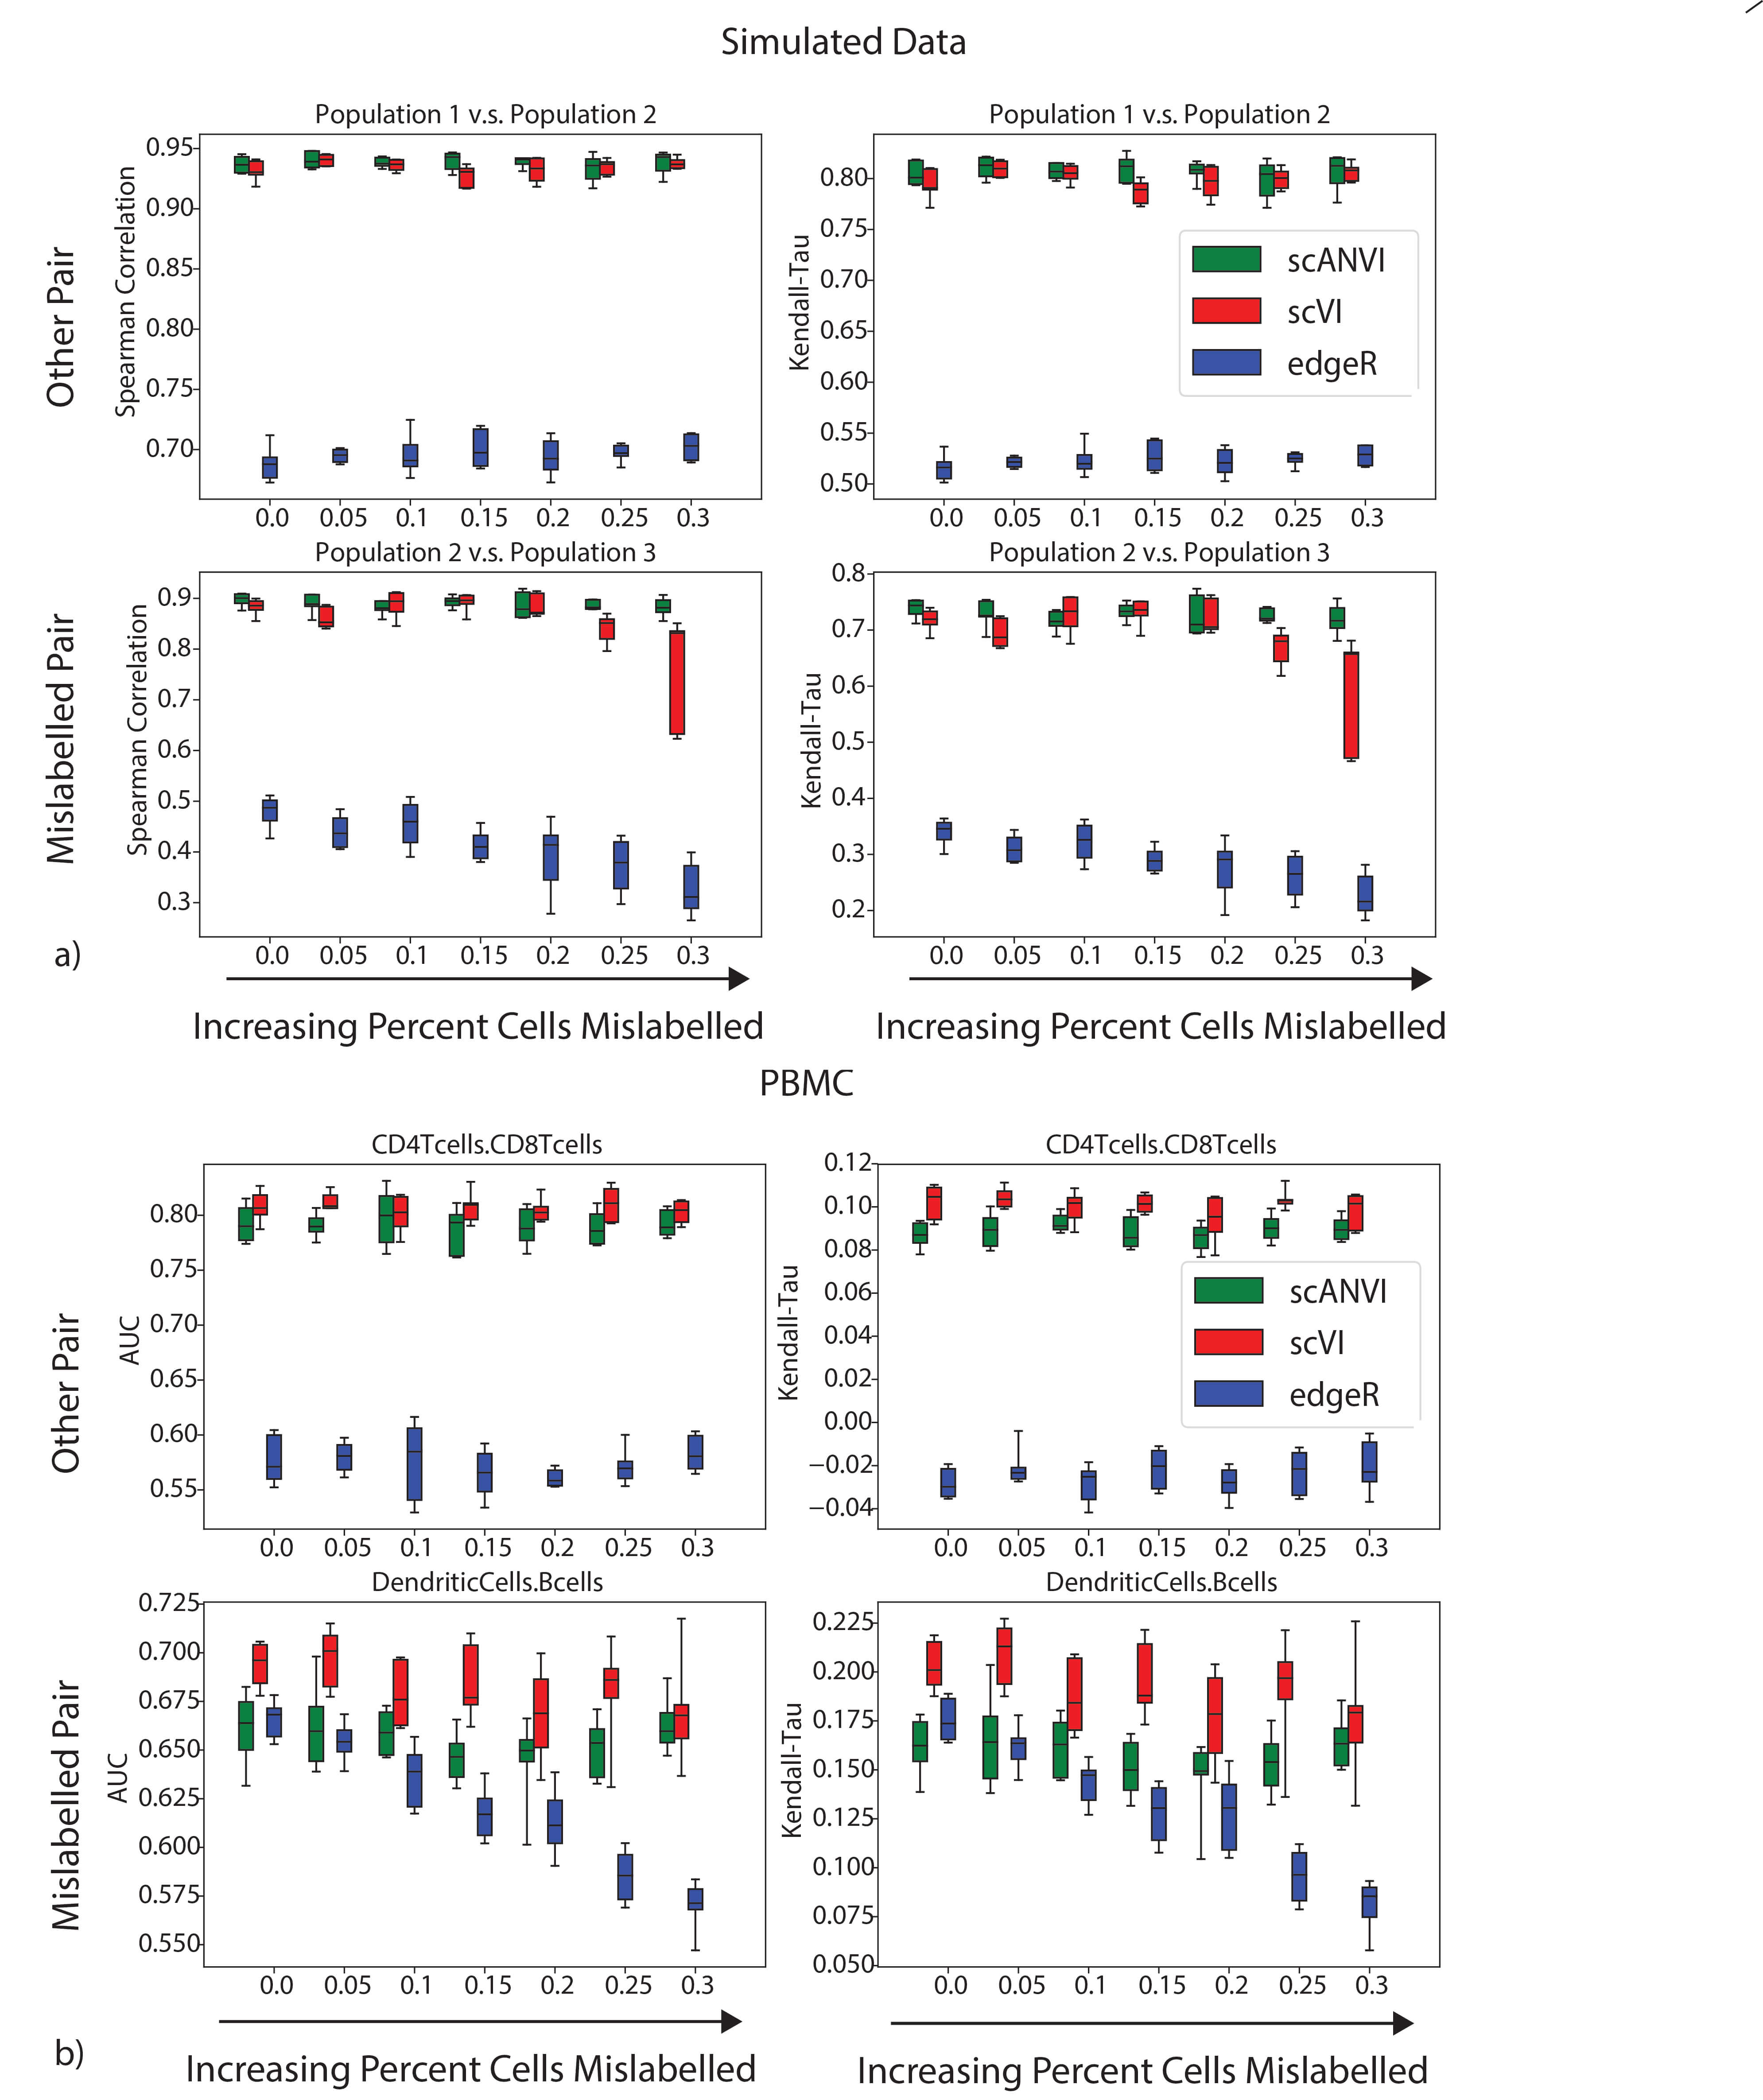
\includegraphics[width=0.9\textwidth]{figures/mislabelled.jpg}
\caption[Mislabeling experiment in differential expression]{Mislabeling experiment in differential expression with $(a)$ PBMC8K and PBMC68K datasets and $(b)$ SymSim simulated datasets. Within each panel: Top: differential expression results for the correctly labeled population pair (CD4 T cells - CD8 T cells in $(a)$ and 1-2 in $(b)$). Bottom: differential expression results for the mislabelled population pair (dendritic cells and B cells in $(a)$ and 2-3 in $(b)$). For all, x-axis represents the proportion of flipped labels. }
\label{scanviDE_mislabel}
\end{suppfigure}
% Combined Labels: 
% \caption

\begin{suppfigure}[H]
\centering
\includegraphics[width=\textwidth]{figures/Nclasses.jpg}
\caption[The effect of the choice of number of classes on the scANVI model]{The effect of the choice of number of classes on the scANVI model likelihood $(a)$, classification accuracy $(b)$ and entropy of batch mixing $(c)$. We trained scANVI using PBMC8K as the labelled dataset, and varied the number of classes in scANVI from 6(true number of labelled cell types) to 14. The thicker line show the mean of 9 replicates, while the colored shading show the 95\% confidence interval. We used a subsampled PBMC8K-CITE dataset, where NK cells are removed from the PBMC8K dataset and B cells are removed from the PBMC-CITE dataset. As we expect, the two unique dataset have low mixing in $(c)$ while the other cell types have high mixing. Although there is no labelled B cells, scANVI does not cluster B cells from the PBMC8K dataset with other cell types in PBMC-CITE. The three metrics we use to evaluate scANVI performance are minimally affected by the increase in the number of classes.  }
\label{scanviNclasses}
\end{suppfigure}

\begin{suppfigure}[H]
\centering
\includegraphics[width=\textwidth]{figures/ZINB_NB.jpg}
\caption[Performance of scVI and scANVI with a negative binomial (NB) distribution]{Performance of scVI and scANVI with a negative binomial (NB) distribution. $(a)$ UMAP plot of the MarrowTM pair using a NB distribution for scVI. $(b)$ Harmonization statistics and differences between regular scVI and NB version (scVI-NB). Dotted lines represent results using scVI-NB. }
\label{scanviZINB_NB}
\end{suppfigure}

\begin{suppfigure}[H]
\centering
\includegraphics[width=0.7\textwidth]{figures/DE_NB.pdf}
\caption[Differential Expression with a negative binomial version of scVI]{Differential Expression with a negative binomial version of scVI. We report all metrics on all pairs of cell types using the simulated dataset previously analyzed as in Figure~\ref{scanvisimulations_panel}a.}
\label{scanviDE_NB}
\end{suppfigure}








\part{Machine Learning for Science}
\label{part2}
\chapter{Information Constraints on Auto-Encoding Variational Bayes}
\chaptermark{HSIC-Constrained VAES}
\label{hcv}
% \input{hsic/0_opening}
\section{Introduction}

Since the introduction of variational auto-encoders (VAEs)~\cite{AEVB},
graphical models whose conditional distribution are specified by deep neural networks have become commonplace.
For problems where all that matters is the goodness-of-fit (e.g., marginal log probability of the data), there is little reason to constrain the flexibility/expressiveness of these networks other than possible considerations of overfitting. In other problems, however, some latent representations may be preferable to others---for example, for reasons of interpretability or modularity.
Traditionally, such constraints on latent representations have been expressed in the graphical model setting via conditional independence assumptions.  But these assumptions are relatively rigid, and with the advent of highly flexible conditional distributions, it has become important to find ways to constrain latent representations that go beyond the rigid conditional independence structures of classical graphical models.

%\todo[inline]{Add some motivation sentences}


In this chapter, we propose a new method for restricting the search space to latent representations
with desired independence properties.
As in~\cite{AEVB}, we approximate the posterior for each observation $X$ with an encoder network that parameterizes $q_\phi(Z \mid X)$.
Restricting this search space amounts to constraining the class of variational distributions that we consider.
In particular, we aim to constrain the \textit{aggregated variational posterior}~\cite{salakhutdinov2010efficient}:
\begin{align}
\hat{q}_\phi(Z) := \mathbb E_{p_{\text{data}}(X)} \left[ q_\phi(Z \mid X) \right].
\end{align}
Here $p_{\text{data}}(X)$ denotes the empirical distribution. 
We aim to enforce independence statements of the form $\hat{q}_\phi(Z^i) \upmodels \hat{q}_\phi(Z^j)$,
where $i$ and $j$ are different coordinates of our latent representation.

Unfortunately, because $\hat{q}_\phi(Z)$ is a mixture distribution, computing any standard measure of independence is intractable, even in the case of Gaussian terms~\cite{Durrieu2012}.
In this chapter, we circumvent this problem in a novel way. First, we estimate dependency though a kernel-based measure of independence, in particular the Hilbert-Schmidt Information Criterion (HSIC)~\cite{Gretton2005}. Second,
by scaling and then subtracting this measure of dependence in the variational lower bound, we get a new variational lower bound on $\log p(X)$.
Maximizing it amounts to maximizing the traditional variational lower bound with a penalty for deviating from the desired independence conditions.
We refer to this approach as \emph{HSIC-constrained VAE} (HCV).

The remainder of the chapter is organized as follows.
In Section~\ref{hsicbackground}, we provide background on VAEs and the HSIC.
In Section~\ref{hsichcv}, we precisely define HCV and provide a theoretical analysis.
The next three sections each present an application of HVC---one for each task shown in Figure~\ref{hsicpgm}.
In Section~\ref{hsicindep}, we consider the problem of learning an interpretable latent representation, and we show that HCV compares favorably to $\beta$-VAE~\cite{Higgins2017} and $\beta$-TCVAE~\cite{betatcVAE}.
In Section~\ref{hsicinvariant}, we consider the problem of learning an invariant representation, showing both that HCV includes the variational fair auto-encoder (VFAE)~\cite{VFAE} as a special case, and that it can improve on the VFAE with respect to its own metrics.
In Section~\ref{hsicdenoise}, we denoise single-cell RNA sequencing data with HCV, and show that our method recovers biological signal better than the current state-of-the-art approach. A open-source implementation of our framework is available on GitHub \url{https://github.com/romain-lopez/HCV}.
\begin{figure}[t!]
\captionsetup[subfigure]{justification=centering}

    \centering
    
    
      \tikzstyle{latent} = [circle,fill=white,draw=black,inner sep=1pt,
minimum size=30pt, font=\fontsize{15}{15}\selectfont, node distance=1]
\tikzstyle{plate caption} = [caption, node distance=0, inner sep=0pt, font=\fontsize{15}{15}\selectfont,
below left=5pt and 0pt of #1.south east] 


  \newcommand{\ltkiz}{1cm}
    
    
    
    \begin{subfigure}[t]{0.3\textwidth}
        \centering   
\tikz{ %
  \node[obs] (x) {${x}$} ; %
  \node[latent, above=0.5 * \ltkiz of x, xshift=+\ltkiz] (u) {${u}$};
    \node[latent, above=0.5 * \ltkiz of x,xshift=-\ltkiz] (v) {${v}$};
    
    \edge {u} {x};
    \edge {v} {x};
  }        
        \caption{Learning Interpretable Representations}
    \end{subfigure}%
    ~
    \begin{subfigure}[t]{0.3\textwidth}
        \centering  
%\scalebox{0.8}        {
        \tikz{ %
  \node[obs] (x) {${x}$} ; %
  \node[obs, above=0.5 * \ltkiz of x, xshift=+\ltkiz] (s) {${s}$};
    \node[latent, above=0.5 * \ltkiz of x,xshift=-\ltkiz] (z) {${z}$};
    
    \edge {z} {x};
    \edge {s} {x};
  }
         
 \caption{Learning Invariant Representations}
    \end{subfigure}
    ~
    \begin{subfigure}[t]{0.30\textwidth}
        \centering  
\tikz{ %
  \node[obs] (x) {${x}$} ; %
  \node[latent, above=0.5 * \ltkiz of x, xshift=2 *\ltkiz] (u) {${u}$};
  \node[obs, below=0.5 * \ltkiz of u, xshift=0] (s) {${s}$};
    \node[latent, above=0.5 * \ltkiz of x,xshift=0] (z) {${z}$};
    
    \edge {z} {x};
    \edge {u} {s};
    \edge {u} {x};
  }   
  
 \caption{
  Learning Denoised Representations}
    \end{subfigure}
    \caption{Tasks presented in the chapter.}
    \label{hsicpgm}
\end{figure}


\section{Background}
\label{hsicbackground}
In representation learning, we aim to transform a variable $x$ into a \emph{representation vector} $z$ for which a given downstream task can be performed more efficiently, either computationally or statistically. For example, one may learn a low-dimensional representation that is predictive of a particular label $y$, as in supervised dictionary learning~\cite{dic_learning}. More generally, a hierarchical Bayesian model~\cite{GelmanHill:2007} applied to a dataset yields stochastic representations, namely, the sufficient statistics for the model's posterior distribution. In order to learn representations that respect specific independence statements, we need to bring together two independent lines of research. First, we will present briefly variational auto-encoders and then non-parametric measures of dependence. 

\subsection{Auto-Encoding Variational Bayes (AEVB)}
We focus on variational auto-encoders~\cite{AEVB} which effectively summarize data for many tasks within a Bayesian inference paradigm~\cite{NIPS2016_6379, Kingma2016}. Let $\{X, S\}$ denote the set of observed random variables and $Z$ the set of hidden random variables (we will use the notation $z^i$ to denote the $i$-th random variable in the set $Z$). Then Bayesian inference aims to maximize the likelihood:
\begin{align}
p_\theta(X \mid S) = \int p_\theta(X \mid Z, S) dp(Z).
\end{align}
Because the integral is in general intractable, variational inference finds a distribution $q_\phi(Z \mid X, S)$ that minimizes a lower bound on the data---the evidence lower bound (ELBO):
\begin{align}
\log p_\theta(X \mid S) \geq \mathbb{E}_{q_\phi(Z \mid X, S)}\log p_\theta(X \mid Z, S) - \kld{(q_\phi(Z|X, S)}{p(Z)}
\end{align}

In auto-encoding variational Bayes (AEVB), the variational distribution is parametrized by a neural network. In the case of a variational auto-encoder (VAE), both the generative model and the variational approximation have  conditional distributions parametrized with neural networks. The difference between the data likelihood and the ELBO is the variational gap:
\begin{align}
	\kld{q_\phi(Z \mid X, S)}{p_\theta(Z \mid X, S)}. 
\end{align}
The original AEVB framework is described in the seminal paper \cite{AEVB} for the case $Z = \{z\}, X = \{x\}, S = \emptyset$. The representation $z$ is optimized to ``explain'' the data $x$. 

AEVB has since been successfully applied and extended. One notable example is the semi-supervised learning case---where $Z = \{z^1, z^2\}$, $X = \{x\}$, $y \in X\cup Z$---which is addressed by the M1 + M2 model~\cite{DBLP:journals/corr/KingmaRMW14}. Here, the representation $z_1$ both explains the original data and is predictive of the label $y$. More generally, solving an additional problem is tantamount to adding a node in the underlying graphical model. Finally, the variational distribution can be used to meet different needs: $q_\phi(y \mid x)$ is a classifier and $q_\phi(z^1 \mid x)$ summarizes the data. 

When using AEVB, the empirical data distribution $p_\text{data}(X, S)$ is transformed into the empirical representation:
\begin{align}
	\hat{q}_\phi(Z) = \mathbb{E}_{p_\text{data}(X, S)}q_\phi(Z \mid X, S).
\end{align}
This mixture is commonly called the aggregated posterior~\cite{Makhzani2015} or average encoding distribution~\cite{Hoffman2016}.


\subsection{Non-parametric estimates of dependence with kernels}

Let $(\Omega, \mathcal{F}, \mathbb{P})$ be a probability space. Let $\mathcal{X}$ (resp. $\mathcal{Y}$) be a separable metric space. Let $u: \Omega \rightarrow \mathcal{X}$ (resp. $v: \Omega \rightarrow \mathcal{Y}$) be a random variable. Let $k: \mathcal{X} \times \mathcal{X} \rightarrow \mathbb{R}$ (resp. $l: \mathcal{Y} \times \mathcal{Y} \rightarrow \mathbb{R}$) be a continuous, bounded, positive semi-definite kernel. Let $\mathcal{H}$ (resp. $\mathcal{K}$) be the corresponding reproducing kernel Hilbert space (RKHS) and $\phi: \Omega \rightarrow \mathcal{H}$ (resp. $\psi:\Omega \rightarrow \mathcal{K}$) the corresponding feature mapping.

Given this setting, one can embed the distribution $P$ of random variable $u$ into a single point $\mu_P$ of the RKHS $\mathcal{H}$ as follows:
\begin{equation}
\mu_{P} = \int_{\Omega} \phi(u) P(du).
\label{hsicembedding}
\end{equation}
If the kernel $k$ is universal\footnote{A kernel $k$ is universal if $k(x,\cdot )$ is continuous for all $x$ and the RKHS induced by $k$ is dense in $C(\mathcal{X})$. This is true for the Gaussian kernel $(u, u') \mapsto e^{-\gamma || u - u'|| ^2}$ when $\gamma > 0$.}, then the mean embedding operator $P \mapsto \mu_P$ is injective~\cite{NIPS2007_3340}. 

We now introduce a kernel-based estimate of \emph{distance} between two distributions $P$ and $Q$ over the random variable $u$. This approach will be used by one of our baselines for learning invariant representations. Such a distance, defined via the canonical distance between their $\mathcal{H}$-embeddings, is called the maximum mean discrepancy~\cite{MMD} and denoted $\text{MMD}(P, Q)$. 

The joint distribution $P(u, v)$ defined over the product space $\mathcal{X} \times \mathcal{Y}$ can be embedded as a point $\mathcal{C}_{uv}$ in the tensor space $\mathcal{H} \otimes \mathcal{K}$. It can also be interpreted as a linear map $\mathcal{H} \rightarrow \mathcal{K}$:
\begin{align}
\forall (f, g) \in \mathcal{H} \times \mathcal{K},~ \mathbb{E}f(u)g(v) = \langle f(u) ,\mathcal{C}_{uv}g(v) \rangle_\mathcal{H} = \langle f\otimes g, \mathcal{C}_{uv}\rangle_{\mathcal{H} \otimes \mathcal{K}}.
\end{align}

Suppose the kernels $k$ and $l$ are universal. The largest eigenvalue of the linear operator $\mathcal{C}_{uv}$ is zero if and only if the random variables $u$ and $v$ are marginally independent~\cite{Gretton2005}. A measure of dependence can therefore be derived from the Hilbert-Schmidt norm of the cross-covariance operator $\mathcal{C}_{uv}$ called the Hilbert-Schmidt Independence Criterion (HSIC)~\cite{HSIC}. Let $(u_i, v_i)_{1 \leq i \leq n}$ denote a sequence of iid copies of the random variable $(u, v)$. In the case where $\mathcal{X} = \mathbb{R}^p$ and $\mathcal{Y} = \mathbb{R}^q$, the V-statistics in Equation~\ref{hsichsic_amp} yield a biased empirical estimate~\cite{NIPS2007_3340}, which can be computed in $\mathcal{O}(n^2(p+q))$ time.
An estimator for HSIC is
\begin{align}\label{hsichsic_amp}
\begin{split}
\hat{\text{HSIC}}_n(P) &= \frac{1}{n^2}\sum_{i, j}^n k(u_i, u_j)l(v_i, v_j) \\
&+ \frac{1}{n^4}\sum_{i, j, k, l}^n k(u_i, u_j)l(v_k, v_l) \\
&- \frac{2}{n^3}\sum_{i, j, k}^n k(u_i, u_j)l(v_i, v_k).
\end{split}
\end{align}

The definition of the cross-covariance operator can be extended to the case of $d$ random variables, simply by adhering to the formal language of tensor spaces. Let $X = (X^1, ..., X^d)$ be a random vector with each component of dimension $p$. The components $X^1, ..., X^d$ are mutually independent if the joint distribution is equal to the tensor product of the marginal distribution. \cite{Pfister2016} derives functional formulation, population statistics and V-statistics for the Hilbert-Schmidt norm of the corresponding generalized cross-covariance operator called $d$HSIC. Notably, under the hypothesis that the canonical kernel from the tensor product $\bigotimes_k\mathcal{H}_k$ is universal, the $d$HSIC is null if and only if the components of the random vector are mutually independent. We write here the retained V-statistics that we will use for the experiments and can compute in time $\mathcal{O}(dn^2p)$:

\begin{equation} \label{hsicdhsic_samp}
\begin{split}
\hat{\text{dHSIC}}_n(P) &= \frac{1}{n^2}\sum_{M_2(n)}\prod_{j=1}^d k^j(x_{i_1}^j, x_{i_2}^j) \\
&+ \frac{1}{n^{2d}}\sum_{M_{2d}(n)}\prod_{j=1}^d k^j(x_{i_{2j-1}}^j, x_{i_{2j}}^j) \\
&- \frac{2}{n^{d+1}}\sum_{M_{d+1}(n)}\prod_{j=1}^d k^j(x_{i_{1}}^j, x_{i_{j+1}}^j)
\end{split}
\end{equation}

The question that naturally follows is when is the canonical kernel from the tensor product $\bigotimes_k\mathcal{H}_k$ universal. \cite{Szabo2017} showed that the characteristic property of the individual kernels is not enough in general. However, in the case of  continuous,
bounded and translation invariant kernels this is a sufficient condition. In subsequent work, we plan to consider the $d$HSIC in this setting.

\section{Theory for HSIC-Constrained VAE (HCV)} 
\label{hsichcv}
This chapter is concerned with intepretability of representations learned via VAEs. Independence between certain components of the representation can aid in interpretability~\cite{betatcVAE, doi:10.1162/neco.1992.4.6.863}. First, we explain why AEVB might not be suitable for learning representations that satisfy independence statements. Second, we present a simple diagnostic in the case where the generative model is fixed. Third, we introduce HSIC-constrained VAEs (HCV): our method to correct approximate posteriors learned via AEVB in order to recover \emph{independent} representations.

\subsection{Independence and representations: Ideal setting}

The goal of learning representation that satisfies certain independence statements can be achieved by adding suitable nodes and edges to the generative distribution graphical model. In particular, marginal independence can be the consequence of an ``explaining away'' pattern as in Figure~\ref{hsicpgm}a for the triplet $\{u, x, v\}$. If we consider the setting of infinite data and an accurate posterior, we find that independence statements in the generative model are respected in the latent representation:

\begin{thm}
\label{hsicvgap}
Let us apply AEVB to a model $p_\theta(X , Z\mid S)$ with independence statement $\mathcal{I}$ (e.g., $z^i \upmodels z^j$ for some $(i, j)$). If the variational gap $\mathbb{E}_{p_\text{data}(X, S)}\kld{q_\phi(Z \mid X, S)}{p_\theta(Z \mid X, S)}$ is zero, then under infinite data the representation $\hat{q}_\phi(Z)$ satisfies statement $\mathcal{I}$.
\end{thm}
\begin{proof}
  Without loss of generality, we can write $\mathcal{I}$ as independence between two variables $Z_i \upmodels Z_j$ for some $(i, j)$. Under infinite data, the empirical distribution $p_\text{data}(X, S)$ is close to $p(X, S)$, the real distribution:
  \begin{align}
  \begin{split}
  \hat{q}_\phi(Z_i, Z_j) & = \int q_\phi(Z_i, Z_j \mid X, S)p_\text{data}(X, S) \\
  &= \int p_\theta(Z_i, Z_j \mid X, S)p_\text{data}(X, S) \\
  &= \int p_\theta(Z_i, Z_j \mid X, S)p(X, S) \\
  &=  p(Z_i, Z_j) \\
  &= p(Z_i)(Z_j).
  \end{split}
  \end{align}
  \end{proof}


In practice we may be far from the idealized infinite setting if $(X, S)$ are high-dimensional. Also, AEVB is commonly used with a naive mean field approximation $q_\phi(Z \mid X, S) = \prod_k q_\phi(z^k \mid X, S)$, which could poorly match the real posterior. In the case of a VAE, neural networks are also used to parametrize the conditional distributions of the generative model. This makes it challenging to know whether naive mean field or any specific improvement~\cite{Kingma2016, BurdaGS15} is appropriate. As a consequence, the aggregated posterior could be quite different from the ``exact'' aggregated posterior $\mathbb{E}_{p_\text{data}(X, S)}p_\theta(Z \mid X, S)$. Notably, the independence properties encoded by the generative model $p_\theta(X \mid S)$ will often not be respected by the approximate posterior. This is observed empirically in~\cite{VFAE}, as well as Section~\ref{hsicindep} and Section~\ref{hsicinvariant} of this work.

\subsection{A simple diagnostic in the case of posterior approximation}

A theoretical analysis explaining why the empirical aggregated posterior presents some misspecified correlation is not straightforward. The main reason is that the learning of the model parameters $\theta$ along with the variational parameters $\phi$ makes diagnosis hard. As a first line of attack, let us consider the case where we approximate the posterior of a fixed model. Consider learning a posterior $q_\phi(Z \mid X, S)$ via naive mean field AEVB. Recent work~\cite{Chen2018,Hoffman2016, Makhzani2015} focuses on decomposing the second term of the ELBO and identifying terms, one of which is the total correlation between hidden variables in the aggregate posterior. This term, in principle, promotes independence. However, the decomposition has numerous interacting terms, which makes exact interpretation difficult. As the generative model is fixed in this setting, optimizing the ELBO is tantamount to minimizing the variational gap, which we propose to decompose as
\begin{equation}
\begin{split}
\kld{q_\phi(Z \mid X, S)}{p_\theta(Z\mid X, S)} =  \sum_k &\kld{q_\phi(z^k\mid X, S)}{p_\theta(z^k\mid X, S)} \\
  &+ \mathbb{E}_{q_\phi(Z\mid X, S)}\log\frac{\prod_k p_\theta(z^k\mid X, S) }{p_\theta(Z\mid X, S)}.
\end{split}
\end{equation}

The last term of this equation quantifies the misspecification of the mean-field assumption. The larger it is, the more the coupling between the hidden variables $Z$. Since neural networks are flexible, they can be very successful at optimizing this variational gap but at the price of introducing supplemental correlation between $Z$ in the aggregated posterior. We expect this side effect whenever we use neural networks to learn a misspecified variational approximation. 

\subsection{Correcting the variational posterior}
We aim to correct the variational posterior $q_\phi(Z \mid X, S)$ so that it satisfies specific independence statements of the form $\forall (i, j) \in \mathcal{S}, \hat{q}_\phi(z^i) \upmodels \hat{q}_\phi(z^j)$. As $\hat{q}_\phi(Z)$ is a mixture distribution, any standard measure of independence is intractable based on the conditionals $q_\phi(Z \mid X, S)$, even in the common case of mixture of Gaussian distributions~\cite{Durrieu2012}. To address this issue, we propose a novel idea: estimate and minimize the dependency via a non-parametric statistical penalty. Given the AEVB framework, let $\lambda \in \mathbb{R}^+$, $\mathcal{Z}_0 = \{z^{i_1}, .., z^{i_p}\} \subset Z$ and $\mathcal{S}_0 = \{s^{j_1}, .., s^{j_q}\} \subset S$. The HCV framework with independence constraints on $\mathcal{Z}_0\cup\mathcal{S}_0 $ learns the parameters $\theta, \phi$ from maximizing the ELBO from AEVB penalized by
\begin{equation} \label{hsicdhsic_penal}
-\lambda d\textrm{HSIC}(\hat{q}_\phi(z^{i_1}, .., z^{i_p})p_\text{data}(s^{j_1}, .., s^{j_q})).
\end{equation}
A few comments are in order regarding this penalty. First, the $d$HSIC is positive and therefore our objective function is still a lower bound on the log-likelihood. The bound will be looser but the resulting parameters will yield a more suitable representation. This trade-off is adjustable via the parameter~$\lambda$. Second, the $d$HSIC can be estimated with the same samples used for stochastic variational inference (i.e., sampling from the variational distribution) and for minibatch sampling (i.e., subsampling the dataset). Third, the HSIC penalty is based only on the variational parameters---not the parameters of the generative model.

\section{Results}
\subsection{Learning interpretable representations}
\label{hsicindep}
Suppose we want to summarize the data $x$ with two independent components $u$ and $v$, as shown in Figure~\ref{hsicpgm}a. The task is especially important for data exploration since independent representations are often more easily interpreted.

A related problem is finding latent factors $(z^1, ..., z^d)$ that correspond to real and interpretable variations in the data. Learning independent representations is then a key step towards learning \emph{disentangled} representations~\cite{betatcVAE, Higgins2017, Kim2018, Chen2016}.
The $\beta$-VAE~\cite{Higgins2017} proposes further penalizing the $\kld{q_\phi(z\mid x)}{p(z)}$ term. It attains significant improvement over state-of-the art methods on real datasets. However, this penalization has been shown to yield poor reconstruction performance~\cite{Burgess2018}. The $\beta$-TCVAE~\cite{betatcVAE} penalized an approximation of the \textit{total correlation} (TC), defined as  $\kld{\hat{q}_\phi(z)}{\prod_k \hat{q}_\phi(z^k)}$ ~\cite{Watanabe}, which is a measure of multivariate mutual independence. However, this quantity does not have a closed-form solution~\cite{Durrieu2012} and the $\beta$-TCVAE uses a biased estimator of the TC---a lower bound from Jensen inequality. That bias will be zero only if evaluated on the whole dataset, which is not possible since the estimator has quadratic complexity in the number of samples. However, the bias from the HSIC~\cite{HSIC} is of order $\mathcal{O}(\nicefrac{1}{n})$; it is negligible whenever the batch-size is large enough. HSIC therefore appears to be a more suitable method to enforce independence in the latent space.

To assess the performance of these various approaches to finding independent representations, we consider a linear Gaussian system, for which exact posterior inference is tractable. Let $(n, m, d) \in \mathbb{N}^3$ and $\lambda \in \mathbb{R}^+$. Let $(A, B) \in \mathbb{R}^{d\times n}\times\mathbb{R}^{d\times m}$ be random matrices with iid normal entries. Let $\Sigma \in \mathbb{R}^{d\times d}$ be a random matrix following a Wishart distribution. Consider the following generative model:
\begin{equation}
\begin{split}
v &\sim \textrm{Normal}(0, I_n) \\
u &\sim \textrm{Normal}(0, I_m) \\
x\mid u, v &\sim \textrm{Normal}(Av + Bu, \lambda I_d + \Sigma).
\end{split}
\end{equation}

The marginal log-likelihood $p(x)$ is tractable:
\begin{equation}
x \sim \textrm{Normal}(0, \lambda I_d + \Sigma + AA^T + BB^T). 
\end{equation}

The complete posterior $p(u, v \mid x)$ is tractable via block matrix inversion, as is the marginal $p(x)$:
\begin{equation}
\begin{split}
V^{-1} &= I_{n+m} + [A, B]^T (\lambda I_d + \Sigma)^{-1} [A, B]  \\
H_\mu &= \Sigma [A, B]^T (\lambda I_d + \Sigma)^{-1} \\
u, v \mid x &\sim \textrm{Normal}(H_\mu x, V). 
\end{split}
\end{equation}

We apply HCV with:
\begin{align}
    Z = \{u, v\}, X = \{x\}, S = \emptyset , \mathcal{Z}_0 = \{u, v\}\text{, and } \mathcal{S}_0 = \emptyset.
\end{align}
This is equivalent to adding to the ELBO the penalty:
\begin{align}
- \lambda \text{HSIC}(\mathbb{E}_{p_\text{data}(x)}q_\phi(u, v\mid x))
\end{align}. We report the trade-off between correlation of the representation and the ELBO for various penalty weights $\lambda$ for each algorithm: $\beta$-VAE~\cite{Higgins2017}, $\beta$-TCVAE~\cite{betatcVAE}, an unconstrained VAE, and HCV. As correlation measures, we consider the summed Pearson correlation $\sum_{(i, j)}\rho(\hat{q}_\phi(u^i), \hat{q}_\phi(v^j))$ and HSIC.

\begin{figure}[ht]
\captionsetup[subfigure]{justification=centering}
    \centering  
    \begin{subfigure}[t]{0.5\textwidth}
        \centering   
		\includegraphics[width=0.7\textwidth]{figures/gaussian.pdf}
    \end{subfigure}%
    ~  
    \begin{subfigure}[t]{0.5\textwidth}
        \centering  
		\includegraphics[width=0.7\textwidth]{figures/gaussian_hsic.pdf}
    \end{subfigure}

    \caption[Results for the linear Gaussian system]{Results for the linear Gaussian system. All results are for a test set. Each dot is averaged across five random seeds. Larger dots indicate greater regularization. The purple line is the log-likelihood under the true posterior. The cyan line is the correlation under the true posterior.}
    %\vspace{-0.5cm}
    \label{hsiclingaussfigure}
\end{figure}

Results are reported in Figure~\ref{hsiclingaussfigure}. The VAE baseline (like all the other methods) has an ELBO value worse than the marginal log-likelihood (horizontal bar) since the real posterior is not likely to be in the function class given by naive mean field AEVB. Also, this baseline has a greater dependence in the aggregated posterior $\hat{q}_\phi(u, v)$ than in the exact posterior $\hat{p}(u, v)$ (vertical bar) for the two measures of correlation. Second, while correcting the variational posterior, we want the best trade-off between model fit and independence. HCV attains the highest ELBO values despite having the lowest correlation. 







\subsection{Learning invariant representations}
\label{hsicinvariant}

\begin{figure}

    
    
      \tikzstyle{latent} = [circle,fill=white,draw=black,inner sep=1pt,
minimum size=30pt, font=\fontsize{15}{15}\selectfont, node distance=1]


  \newcommand{\ltkiz}{1cm}
  
  
\captionsetup[subfigure]{justification=centering}
    \centering  
    \begin{subfigure}[t]{0.3\textwidth}
        \centering   
		\includegraphics[width=3cm]{figures/angles.pdf}
        \caption{$s$: angle between the camera and the light source}
    \end{subfigure}%
    ~ 
    \begin{subfigure}[t]{0.3\textwidth}
        \centering  
		\includegraphics[width=0.7\textwidth]{figures/face.pdf}
        \caption{One image $x$ for a given lighting condition $s$ and person $y$}
    \end{subfigure}
        ~ 
    \begin{subfigure}[t]{0.3\textwidth}
        \centering  
        \scalebox{0.65}
        {
\tikz{ %
  \node[obs] (x) {${x}$} ; %
  \node[obs, above=0.5 * \ltkiz of x, xshift=+1.5\ltkiz] (s) {${s}$};
    \node[latent, above=0.5 * \ltkiz of x,xshift=0*\ltkiz] (z1) {${z_1}$};
      \node[obs, above=0.5 * \ltkiz of z1, xshift=+1.5\ltkiz] (y) {${y}$};
    \node[latent, above=0.5 * \ltkiz of z1,xshift=0*\ltkiz] (z2) {${z_2}$};    
    \edge {z1} {x};
    \edge{z2} {z1};
    \edge {y} {z1};
    \edge {s} {x};
} }
 \caption{Complete graphical model}
    \end{subfigure}
        \caption{Framework for learning invariant representations in the Extended Yale B Face dataset.}
    \label{hsicyale}
\end{figure}


We now consider the particular problem of learning representations for the data that is \emph{invariant} to a given nuisance variable. As a particular instance of the graphical model in Figure~\ref{hsicpgm}b, we embed an image $x$ into a latent vector $z_1$ whose distribution is independent of the observed lighting condition $s$ while being predictive of the person identity $y$ (Figure~\ref{hsicyale}). The generative model is defined in Figure~\ref{hsicyale}c and the variational distribution decomposes as:
\begin{align}
     q_\phi(z^1, z^2 \mid x, s, y) = q_\phi(z^1 \mid x, s)q_\phi(z^2 \mid z^1, y),
\end{align}
as in~\cite{VFAE}. This problem has been studied in~\cite{VFAE} for binary or categorical $s$. For their experiment with a continuous covariate $s$, they discretize $s$ and use the MMD to match the distributions $\hat{q}_\phi(z^1 \mid s=0)$ and $\hat{q}_\phi(z^1 \mid s=j)$ for all $j$. Perhaps surprisingly, their penalty turns out to be a special case of our HSIC penalty.

\begin{thm}
\label{hsicmmd_hsic}
Let the nuisance factor $s$ be a discrete random variable and let $l$ (the kernel for $\mathcal{K}$) be a Kronecker delta function $\delta: (s, s') \mapsto \mathds{1}_{s = s'}$. Then, the V-statistic corresponding to $\textrm{HSIC}
(\hat{q}_\phi(z^1), p_{\text{data}})$ is a weighted sum of the V-statistics of the MMD between the pairs $\hat{q}_\phi(z \mid s=i), \hat{q}_\phi(z \mid s=j)$. The weights are functions of the empirical probabilities for $s$.
\end{thm}
\begin{proof}
     The proof relies on sum manipulations. First, we carefully write the case where $s$ is binary without loss of generality. Let us assume $M$ samples from the joint $(x, s)$ and let us reorder them such that $s_0 = ... = s_N = 0$ and $s_{N+1} = ... = s_M = 1$. In that case,
     
     \begin{align*}
     \begin{split}
          \textrm{HSIC} &=  \frac{1}{M^2}\sum_{ij}^M k_{ij}l_{ij} + \frac{1}{M^4}\sum_{ijkl}^M k_{ij}l_{kl} - \frac{2}{M^3}\sum_{ijk}^M k_{ij}l_{ik} \\ ~ \\
          \textrm{HSIC} &= \frac{1}{M^2}\sum_{i=0}^N\sum_{j=0}^N k_{ij} + \sum_{i=N+1}^M\sum_{j=N+1}^M k_{ij} + \frac{N^2 + (M-N+1)^2}{M^4}\sum_{ij}^M k_{ij} \\
     &- \frac{2}{M^3}\left(N \sum_{i=0}^N \sum_j^M k_{ij} + (M-N+1) \sum_{i=N+1}^M \sum_j^M k_{ij} \right) \\ ~ \\
     \textrm{HSIC} &= \frac{(M-N+1)^2}{M^4} \sum_{i=0, j=0}^Nk_{ij} + \frac{N^2}{M^4} \sum_{i=N+1, j=N+1}^M k_{ij} -2 \frac{N(M-N+1)}{M^4} \sum_{i=0}^N\sum_{j=N+1}^M k_{ij} \\~\\
     \textrm{HSIC} &= \frac{N^2(M-N+1)^2}{M^4} \left( \frac{1}{N^2}\sum_{i=0, j=0}^Nk_{ij} + \frac{1}{(M-N+1)^2} \sum_{i=N+1, j=N+1}^M k_{ij}\right.  \\
     &\qquad\qquad  \left. -2 \frac{1}{N(M-N+1)} \sum_{i=0}^N\sum_{j=N+1}^M k_{ij}\right).
     \end{split}
     \end{align*}
     Above,  the term inside the parenthesis is the V-statistic for the MMD between $q(z \mid  s=0)$ and $q(z \mid s=1)$. In the general case of $s$ discrete, we then have a sum of MMD weighted by the values of the empirical $p(s)$.
     \end{proof}

Working with the HSIC rather than an MMD penalty lets us avoid discretizing $s$. We take into account the whole angular range and not simply the direction of the light. We apply HCV with mean-field AEVB, $Z = \{z^1, z^2\}, X = \{x, y\}, S = \{s\}, \mathcal{Z}_0 = \{z^1\}$ and $\mathcal{S}_0 = \{s\}$.


\paragraph{Dataset}
The extended Yale B dataset~\cite{YALEB} contains cropped faces~\cite{KCLee05} of 38 people under 50 lighting conditions. These conditions are unit vectors in $\mathbb{R}^3$ encoding the direction of the light source and can be summarized into five discrete groups (upper right, upper left, lower right, lower left and front). Following \cite{VFAE}, we use one image from each group per person (total 190 images) and use the remaining images for testing. The task is to learn a representation of the faces that is good at identifying people but has low correlation with the lighting conditions.

\paragraph{Experiment}
We repeat the experiments from the paper introducing the variational fair auto-encoder (VFAE)~\cite{VFAE}, this time comparing the VAE~\cite{AEVB} with no covariate $s$, the VFAE~\cite{VFAE} with observed lighting direction groups (five groups), and the HCV with the lighting direction vector (a three-dimensional vector). As a supplemental baseline, we also report results for the unconstrained VAEs. As in~\cite{VFAE}, we report 1) the accuracy for classifying the person based on the variational distribution $q_\phi(y \mid z^1, s)$; 2) the classification accuracy for the lighting group condition (five-way classification) based on a logistic regression and a random forest classifier on a sample from the variational posterior $q_\phi(z^1 \mid z^2, y, s)$ for each datapoint; and 3) the average error for predicting the lighting direction with linear regression and a random forest regressor, trained on a sample from the variational posterior $q_\phi(z^1 \mid z^2, y, s)$. Error is expressed in degrees. $\lambda$ is optimized via grid search as in~\cite{VFAE}. 

We report our results in Table~\ref{hsicYale}. As expected, adding information (either the lightning group or the refined lightning direction) always improves the quality of the classifier $q_\phi(y \mid z^1, s)$. This can be seen by comparing the scores between the vanilla VAE and the unconstrained algorithms. However, by using side information $s$, the unconstrained models yield a representation less suitable because it is more correlated with the nuisance variables. There is therefore a trade-off between correlation to the nuisance and performance. Our proposed method (HCV) shows greater invariance to lighting direction while accurately predicting people's identities.


\begin{table}[ht]
\centering
\begin{small}
\begin{tabular}{lccccc}
\toprule
     & \multirow{2}{*}{\begin{tabular}[c]{@{}c@{}}\vspace{-0.1cm}\\ \textbf{Person identity}\\ \textbf{(Accuracy)}\end{tabular}} & \multicolumn{2}{c}{\begin{tabular}[c]{@{}c@{}}\textbf{Lighting group}\\ \textbf{(Average classification error)}\end{tabular}}                                             & \multicolumn{2}{c}{\begin{tabular}[c]{@{}c@{}}\textbf{Lighting direction}\\ \textbf{(Average error in degree)}\end{tabular}}                       \\[0.2 cm]
     &                                                                                       & \begin{tabular}[c]{@{}c@{}}\textbf{Random Forest}\\ \textbf{Classifier}\end{tabular} & \begin{tabular}[c]{@{}c@{}}\textbf{Logistic} \\ \textbf{Regression}\end{tabular} & \begin{tabular}[c]{@{}c@{}}\textbf{Random Forest}\\ \textbf{Regressor}\end{tabular} & \begin{tabular}[c]{@{}c@{}}\textbf{Linear} \\ \textbf{Regression}\end{tabular} \\
     \midrule
\textbf{VAE}  & 0.72                                                                                  & 0.26                                                               & 0.11                                                           & 14.07                                                             & 9.40                                                         \\
\textbf{VFAE}$^*$ & 0.74                                                                                  & 0.23                                                               & 0.01                                                           & 13.96                                                             & 8.63                                                        \\
\textbf{VFAE} & 0.69                                                                                  & 0.51                                                               & \textbf{0.42}                                                           & 23.59                                                             & 19.89                                                        \\
\textbf{HCV}$^*$  & \textbf{0.75}                                                                                  & 0.25                                                               & 0.10                                                           & 12.25                                                             & 2.59 \\
\textbf{HCV}  & \textbf{0.75}                                                                                  & \textbf{0.52}                                                               & 0.29                                                           & \textbf{36.15}                                                             & \textbf{28.04} \\
\bottomrule
\end{tabular}
\end{small}
\caption[Results on the Extended Yale B dataset]{Results on the Extended Yale B dataset. Preprocessing differences likely explain the slight deviation in scores from~\cite{VFAE}. Stars ($^*$) the unconstrained version of the algorithm was used.}
\label{hsicYale}
\end{table}
%\end{wraptable}

\subsection{Learning denoised representations}
\label{hsicdenoise}
This section presents a case study of denoising datasets in the setting of an important open scientific problem. The task of \emph{denoising} consists of representing experimental observations $x$ and nuisance observations $s$ with two independent signals: biological signal $z$ and technical noise $u$. The difficulty is that $x$ contains both biological signal and noise and is therefore strongly correlated with $s$ (Figure~\ref{hsicpgm}c). In particular, we focus on single-cell RNA sequencing (scRNA-seq) data which renders a gene-expression snapshot of an heterogeneous sample of cells. Such data can reveal a cell's type~\cite{Wagner2016, Tanay2017}, if we can cope with a high level of technical noise~\cite{Grun2014}.


\subsubsection{Data presentation}
The output of an scRNA-seq experiment is a list of transcripts $(l_m)_{m \in \mathcal{M}}$. Each transcript $l_m$ is an mRNA molecule enriched with a cell-specific barcode and a unique molecule identifier, as in \cite{Klein2015}. Cell-specific barcodes enable the biologist to work at single-cell resolution. Unique molecule identifiers (UMIs) are meant to remove some significant part of the technical bias (e.g., amplification bias) and make it possible to obtain an accurate probabilistic model for these datasets~\cite{Lopez292037}. Transcripts are then aligned to a reference genome with tools such as CellRanger~\cite{Zheng2017}.

The data from the experiment has two parts. First, there is a gene expression matrix $(X_{ng})_{(n, g) \in \mathcal{N}\times\mathcal{G}}$, where $\mathcal{N}$ designates the set of cells detected in the experiment and $\mathcal{G}$ is the set of genes the transcripts have been aligned with. A particular entry of this matrix indicates the number of times a particular gene has been expressed in a particular cell. Second, we have quality control metrics $(s^i)_{i\in \mathcal{S}}$ which assess the level of errors and corrections in the alignment process:
\begin{itemize}
\item $s^1$: proportion of transcripts which confidently mapped to a gene;
\item $s^2$: proportion of transcripts mapping to the genome, but not to a gene;
\item $s^3$: proportion of transcripts which did not align;
\item $s^4$: proportion of transcripts whose UMI sequence was corrected by the alignment procedure;
\item $s^5$:~proportion of transcripts whose barcode sequence was corrected by the alignment procedure.
\end{itemize}
These metrics cannot be described with a generative model as easily as gene expression data but they nonetheless impact a significant number of tasks in the research area~\cite{Cole2017}. Another significant portion of these metrics focus on the sampling effects (i.e., the discrepancy in the total number of transcripts captured in each cell) which can be taken into account in a principled way in a graphical model as in~\cite{Lopez292037}. 

\begin{figure}[h!]

    
    
      \tikzstyle{latent} = [circle,fill=white,draw=black,inner sep=1pt,
minimum size=30pt, font=\fontsize{15}{15}\selectfont, node distance=1]


  \newcommand{\ltkiz}{1cm}
  
  
\captionsetup[subfigure]{justification=centering}
    \centering  
    \begin{subfigure}[t]{0.3\textwidth}
        \centering   
		\includegraphics[width=3.5cm]{figures/cell_types.pdf}
        \caption{Embedding of $x$: gene expression data. Each point is a cell. Colors are cell-types.}
    \end{subfigure}%
    ~  
    \begin{subfigure}[t]{0.3\textwidth}
        \centering  
		\includegraphics[width=0.7\textwidth]{figures/qc.pdf}
        \caption{Embedding of $s$: alignment errors. Each point is a cell. Color is $s^1$.}
    \end{subfigure}
    ~
    \begin{subfigure}[t]{0.3\textwidth}
        \centering  
		\includegraphics[width=0.7\textwidth]{figures/qc_5.pdf}
        \caption{Embedding of $x$: gene expression data. Each point is a cell. Color is the same quality control metric $s^1$.}
    \end{subfigure}

        \caption[Raw data from the PBMC dataset]{Raw data from the PBMC dataset. $s^1$ is the proportion of transcripts which confidently mapped to a gene for each cell.}
    \label{hsicpbmc}
\end{figure}


We visualize these datasets $x$ and $s$ with tSNE~\cite{Hinton2008} in Figure~\ref{hsicpbmc}. Note that $x$ is correlated with $s$, especially within each cell type. A common application for scRNA-seq is discovering cell types, which can be be done without correcting for the alignment errors~\cite{Wang2017}. A second important application is identifying genes that are more expressed in one cell type than in another---this hypothesis testing problem is called \emph{differential expression}~\cite{deseq2, mast}. Not modeling $s$ can induce a dependence on $x$ which hampers hypothesis testing~\cite{Cole2017}. 

\subsubsection{Deep generative model}

Most research efforts in scRNA-seq methodology research focus on using generalized linear models and two-way ANOVA~\cite{Risso2017,Cole2017} to regress out the effects of quality control metrics. However, this paradigm is incompatible with hypothesis testing. A generative approach, however, would allow marginalizing out the effect of these metrics, which is more aligned with Bayesian principles. Our main contribution is to incorporate these alignment errors into our graphical model to provide a better Bayesian testing procedure. We apply HCV with $Z = \{z, u\}, X=\{x, s\}, \mathcal{Z}_0 = \{z, u\}$. By integrating out $u$ while sampling from the variational posterior, $\int q_\phi(x \mid z, u)dp(u)$, we find a Bayes factor that is not subject to noise.


\begin{figure}[h]
  \centering
  \tikzstyle{latent} = [circle,fill=white,draw=black,inner sep=1pt,
minimum size=30pt, font=\fontsize{15}{15}\selectfont, node distance=1]
\tikzstyle{plate caption} = [caption, node distance=0, inner sep=0pt, font=\fontsize{12}{12}\selectfont,
below left=5pt and 0pt of #1.south east] %

\tikzstyle{second plate caption} = [caption, node distance=0, inner sep=0pt, font=\fontsize{12}{12}\selectfont, below left=5pt and 0pt of #1.south west] %
% \plate [options] {name} {fitlist} {caption} {text}
\renewcommand{\plate}[5][]{ %
  \node[wrap=#3] (#2-wrap) {}; %
  \node[plate caption=#2-wrap] (#2-caption) {#4}; %
  \node[second plate caption=#2-wrap] (#2-caption) {#5}; %
  \node[plate=(#2-wrap)(#2-caption), #1] (#2) {}; %
}


  \newcommand{\ltkiz}{1.5cm}
  
  \scalebox{0.7} {
  \tikz{ %
  \node[obs] (x) {${x}_{ng}$} ; %
  \node[obs, right=2 * \ltkiz of x] (s) {${s}_{nj}$} ; 
  \node[latent, above=0.5 * \ltkiz of x, xshift=\ltkiz] (h) {${h}_{ng}$};
  \node[latent, above=0.5 * \ltkiz of x, xshift=-\ltkiz]  (y) {${y}_{ng}$};
  \node[latent, above=0.5 * \ltkiz of y] (w) {${w}_{ng}$};
    \node[latent, above=0.5 * \ltkiz of w, xshift=-\ltkiz] (l) {${l}_{n}$};
  \node[latent, above=0.5 * \ltkiz of w, xshift=\ltkiz] (z) {${z}_{n}$};
  \node[latent, above=0.5 * \ltkiz of w, xshift=3*\ltkiz] (u) {${u}_{n}$};
  \node[det, above=3* \ltkiz of y, xshift=0*\ltkiz] (t) {$\theta$};
    \node[det, fill=gray!25, above=3* \ltkiz of y, xshift=-1*\ltkiz] (lm) {$l_\mu$};
    \node[det, fill=gray!25, above=3* \ltkiz of y, xshift=-2*\ltkiz] (lv) {$l_\sigma$};

    \plate[inner sep=0.30cm, xshift=-0.cm, yshift=0.cm] {plate1} {(w) (h) (y) (x)} {G} {Genes}; %
    \plate[inner sep=0.30cm, xshift=-0.cm, yshift=0.cm] {plate2} {(s)} {J} {QC};
   \plate[inner sep=0.30cm, xshift=-0.cm, yshift=0.cm] {plate3} {(z) (l) (w) (h) (y) (x) (s) (u) (plate1) (plate2)} {N} {Cells}; %
    \edge {lm} {l};
    \edge {lv} {l};
    \edge {t} {w} ;
    \edge {z} {w} ; %
    \edge {l} {y};
    \edge {h} {x} ; %
    \edge {w} {y}; %
    \edge {y} {x} ; %
    \edge {u} {s};
    \edge {u} {h};
    \edge {u} {w};
  }
  }
\caption[Our proposed modification of the scVI graphical model]{Our proposed modification of the scVI graphical model. Shaded vertices represent observed random variables. Empty vertices represent latent random variables. Shaded diamonds represent constants, set a priori. Empty diamonds represent global variables shared across all genes and cells. Edges signify conditional dependency. Rectangles (``plates'') represent independent replication. }
\label{hsicgraph}
\end{figure}

\paragraph{Generative model}
Our probabilistic model is a modification of the single-cell Variational Inference model~\cite{Lopez292037}. The main difference is the addition of latent variable $u$ and the node for the sequencing errors $s$ (Figure~\ref{hsicgraph}). Let $\ell_\mu, \ell_\sigma \in \mathbb{R}_+^B$ and $\theta \in \mathbb{R}_+^G$. Let $f_w$ (resp. $f_h, f_{\mu_s}$ and $f_{\sigma_s}$) be a neural network with exponential (resp. sigmoid, sigmoid and exponential) link function. Each datapoint $(x_n, s_n)$ is generated according to the following model. First, we draw the latent variables we wish to perform inference over:
\begin{align}
	z_n &\sim \textrm{Normal}(0, I) \\
    u_n &\sim \textrm{Normal}(0, I) \\
    \ell_n &\sim \textrm{LogNormal}(\ell_\mu, \ell_\sigma^2) 
\end{align}

$z$ will encode the biological information, $u$ the technical information from the alignment process and $l$ the sampling intensity. Then, we have some intermediate hidden variables useful for testing and model interpretation that we will integrate out for inference:
\begin{align}
    w_{ng} &\sim \textrm{Gamma}(f_w^g(z_n, u_n), \theta) \\
    y_{ng} &\sim \textrm{Poisson}( \ell_n w_{ng}) \\
    h_{ng} &\sim \textrm{Bernoulli}(f_h^g(u_n)) 
\end{align}

Physically, $w_{ng}$ represents the average proportion of transcripts aligned with gene $g$ in cell $n$. $y_{ng}$ represents one outcome of the sampling process. $h_{ng}$ represents some additional control for the zeros that come from alignment. Finally, the observations fall from:
\begin{align}
    x_{ng} &=
\begin{cases}
y_{ng} & \text{ if } h_{ng} = 0,\\
0 & \text{ otherwise}.
\end{cases} \\
s_{nj} &\sim \textrm{Normal}(f_{\mu_s}^j(u_n), f_{\sigma_s}^j(u_n)) 
\end{align}

where we constrained the mean $f_{\mu_s}^j(u_n)$ to be in the 0-1 range since $s$ is a vector of individual proportions. This model is a very competitive solution for representing single-cell RNA sequencing data.

\paragraph{Variational approximation to the posterior}

Applying AEVB with $X = \{x, s\}, Z = \{z, l, u, w, y, h\}$ seems doomed to fail since some of the variables are discrete. Fortunately, variables $\{w, y, h\}$ can be integrated out analytically: $p(x \mid l, z, u)$ is a Zero-Inflated Negative Binomial distribution. We then apply AEVB with $X = \{x, s\}, Z = \{z, l, u\}$ with the mean-field variational posterior:
\begin{align}
  q_\phi(z, l, u \mid x, s) = q_\phi(z \mid x)q_\phi(l \mid x)q_\phi(u \mid x, s).
\end{align} 

The evidence lower bound is
\begin{equation}
\begin{split}
\log p_\theta(x, s) &\geq \mathbb{E}_{q_\phi(z \mid x)q_\phi(l \mid x)q_\phi(u \mid x, s)}\log p_\theta(x \mid l, z, u) + \mathbb{E}_{q_\phi(u \mid x, s)}\log p_\theta(s \mid u) \\
&- \kld{q_\phi(z \mid x)}{p(z)}- \kld{q_\phi(l \mid x)}{p(l)} - \kld{q_\phi(u \mid x, s)}{p(u)}
\end{split}
\end{equation}

When using the reparametrization trick~\cite{AEVB}, all the resulting quantities can be analytically derived and differentiated. Parameters $\ell_\mu, \ell_\sigma^2$ are set to the mean and average of the number of molecules in all cells of the data (in log-scale). Parameters $\theta$ are learned with variational Bayes, and treated as global variables in the training procedure.

\paragraph{Bayesian hypothesis testing}
We capitalize on our careful modeling to perform principled differential expression. Given two sets of samples $\{x_a \mid a \in A\}$ and $\{x_b \mid b \in B\}$, we would like to test whether a particular gene $g$ is more expressed in population $A$ or in population $B$. 
More formally, for each gene $g$ and a pair of cells $(z_a, u_a)$, $(z_b, u_b)$ with observed gene expression $(x_a, x_b)$ and quality control metrics $(s_a, s_b)$, we can formulate two models of the world under which one of the following hypotheses is true:

$$\mathcal{H}_1^g:= \mathbb{E}f_w^g(z_a, u) > \mathbb{E}f_w^g(z_b, u) \textrm{~~~~vs.~~~~} \mathcal{H}_2^g:=\mathbb{E}f_w^g(z_a, u) \leq \mathbb{E}f_w^g(z_b, u)$$

Where the expectation is taken over $u$ to integrate out the technical variation. Evaluating the likelihood ratio test for whether our datapoints $(x_a, x_b), (s_a, s_b)$ are more probable under the first hypothesis is equivalent to writing a Bayes factor:
\begin{align}
  K = \log_e \frac{p(\mathcal{H}_1^g \mid x_a, x_b)}{p(\mathcal{H}_2^g \mid x_a, x_b)}
\end{align} 

where the posterior of these models can be approximated via the variational distribution:
\begin{align}
  p(\mathcal{H}_1^g \mid x_a, x_b) \approx \mathbb{E}_{\bar{q}} p(f_w^g(z_a, u_a) \leq f_w^g(z_b, u_b) ),
\end{align} 
where $\bar{q} = q(z_a \mid x_a)q(z_b \mid x_b)p(u_a)p(u_b)$. Remarkably, we can use Monte Carlo integration to compute these integrals because all the measures have low dimension.


\paragraph{Dataset} We considered scRNA-seq data from peripheral
blood mononuclear cells (PBMCs) from a healthy donor \cite{Zheng2017}. Our dataset includes 12,039 cells and 3,346 genes, five quality control metrics from CellRanger and cell-type annotations extracted with Seurat~\cite{SEURAT}. We preprocessed the data as in \cite{Lopez292037,Cole2017}. Our ground truth for the hypothesis testing, from microarray studies, is a set of genes that are differentially expressed between human B cells and dendritic cells (n=10 in each group~\cite{Nakaya2011}).

\paragraph{Experiment} 
We compare scVI~\cite{Lopez292037}, a state-of-the-art model, with no observed nuisance variables ($8$ latent dimensions for $z$), and our proposed model with observed quality control metrics. We use five latent dimensions for $z$ and three for $u$. The penalty $\lambda$ is selected through grid search. For each algorithm, we report 1) the coefficient of determination of a linear regression and random forest regressor for the quality metrics predictions based on the latent space, 2) the irreproducible discovery rate (IDR)~\cite{Li2011} model between the Bayes factor of the model and the p-values from the micro-array. The mixture weights, reported in~\cite{Lopez292037}, are similar between the original scVI and our modification (and therefore higher than other mainstream differential expression procedures) and saturate the number of significant genes in this experiment ($\sim$23\%). We also report the correlation of the reproducible mixture as a second-order quality metric for our gene rankings. 

We report our results in Table~\ref{hsicPBMC}. First, the proposed method efficiently removes much correlation with the nuisance variables $s$ in the latent space $z$. Second, the proposed method yields a better ranking of the genes when performing Bayesian hypothesis testing. This is shown by a substantially higher correlation coefficient for the IDR, which indicates the obtained ranking better conforms with the micro-array results. Our denoised latent space is therefore extracting information from the data that is less subject to alignment errors and more biologically interpretable.

\begin{table}[ht]
\centering
\begin{small}
\begin{tabular}{lcccc}
\toprule
      & \multicolumn{2}{c}{\begin{tabular}[c]{@{}c@{}}\textbf{Irreproducible Discovery Rate}\end{tabular}}
      
      %\multirow{2}{*}{\begin{tabular}[c]{@{}c@{}}\vspace{-0.1cm}\\Mixture weights of\\ reproducible genes\end{tabular}} & \multirow{2}{*}{\begin{tabular}[c]{@{}c@{}}\vspace{-0.1cm}\\Rank correlation of\\ reproducible genes\end{tabular}}
      & \multicolumn{2}{c}{\begin{tabular}[c]{@{}c@{}}\textbf{Quality control metrics}\\ \textbf{(coefficient of determination)}\end{tabular}}             \\
                                                                                            & \begin{tabular}[c]{@{}c@{}}\textbf{Mixture}\\\textbf{weight}\end{tabular}    &               \begin{tabular}[c]{@{}c@{}}\textbf{Reproducible}\\ \textbf{correlation}\end{tabular}                                                                                    & \begin{tabular}[c]{@{}c@{}}\textbf{Linear}\\\textbf{Regression}\end{tabular} & \begin{tabular}[c]{@{}c@{}}\textbf{Random Forest}\\ \textbf{Regression}\end{tabular} \\
          \midrule

\textbf{scVI} & \textbf{0.213~$\pm$~0.001} & 0.26~$\pm$~0.07    & 0.195    & 0.129  \\
\textbf{HCV}  & \textbf{0.217~$\pm$~0.003} &\textbf{0.43~$\pm$~0.02}     & \textbf{0.176}    & \textbf{0.123}  \\
\bottomrule
\end{tabular}
\end{small}
\caption[Results on the PBMCs dataset]{Results on the PBMCs dataset. IDR results are averaged over twenty initializations.}
\label{hsicPBMC}
\end{table}

\section{Discussion}
We have presented a flexible framework for correcting independence properties of aggregated variational posteriors learned via naive mean field AEVB. The correction is performed by penalizing the ELBO with the HSIC---a kernel-based measure of dependency---between samples from the variational posterior. 

We illustrated how variational posterior misspecification in AEVB could unwillingly promote dependence in the aggregated posterior. Future work should look at other variational approximations and quantify this dependence. 

Penalizing the HSIC as we do for each mini-batch implies that no information is learned about distribution $\hat{q}(Z)$ or $\prod_i{\hat{q}(z^i)}$ during training. On one hand, this is positive since we do no have to estimate more parameters, especially if the joint estimation would imply a minimax problem as in~\cite{Kim2018, Makhzani2015}. One the other hand, that could be harmful if the HSIC could not be estimated with only a mini-batch. Our experiments show this does not happen in a reasonable set of configurations.

Trading a minimax problem for an estimation problem does not come for free. First, there are some computational considerations. The HSIC is computed in quadratic time but linear time estimators of dependence~\cite{Jitkrittum2016} or random features approximations~\cite{Perez-Suay2018} should be used for non-standard batch sizes. For example, to train on the entire extended Yale B dataset, VAE takes two minutes, VFAE takes ten minutes, and HCV takes three minutes (VFAE is slower because of the discrete operation it has to perform to form the samples for estimating the MMD). Second, the problem of choosing the best kernel is known to be difficult~\cite{Flaxman2016}. In the experiments, we rely on standard and efficient choices: a Gaussian kernel with median heuristic for the bandwidth. The bandwidth can be chosen analytically in the case of a Gaussian latent variable and done offline in case of an observed nuisance variable. Third, the general formulation of HCV with the $d$HSIC penalization, as in Equation~\ref{hsicdhsic_penal}, should be nuanced since the V-statistic relies on a U-statistic of order $2d$. Standard non-asymptotic bounds as in~\cite{Gretton2005} would exhibit a concentration rate of $\mathcal{O}(\sqrt{\nicefrac{d}{n}})$ and therefore not scale well for a large number of variables.

We also applied our HCV framework to scRNA-seq data to remove technical noise. The same graphical model can be readily applied to several other problems in the field. For example, we may wish to remove cell cycles~\cite{Florian2015} that are biologically variable but typically independent of what biologists want to observe. We hope our approach will empower biological analysis with scalable and flexible tools for data interpretation.

\chapter{Decision-making with Auto-Encoding Variational Bayes}
\chaptermark{Decision-making with AEVB}
\label{decision}
% \input{decision/0_opening.tex}
\section{Introduction}

The auto-encoding variational Bayes (AEVB) algorithm relies on neural networks to amortize approximate inference and
performs model selection by maximizing a lower bound on the model evidence~\cite{AEVB, Rezende2014}. In the specific case of variational autoencoders (VAEs), a low-dimensional representation of data is transformed through a learned nonlinear function (another neural network) into the parameters of a conditional likelihood. VAEs achieve impressive performance on pattern-matching tasks like representation/manifold learning and synthetic image generation~\cite{Gulrajani2017}.

Many machine learning applications, however, require decisions, not just compact representations of the data. 
Researchers have accordingly attempted to use VAEs for decision-making applications, including novelty detection in control applications~\cite{Amini2018}, mutation-effect prediction from genomic sequences~\cite{Riesselman2018}, artifact detection~\cite{Ding2018}, and Bayesian hypothesis testing for single-cell RNA sequencing data~\cite{Lopez292037, Xu2019}.
To make decisions based on VAEs, these researchers implicitly appeal to Bayesian decision theory, which counsels taking the action that minimizes expected loss under the posterior distribution~\cite{Fienberg}.

However, for VAEs, the relevant functionals of the posterior cannot be computed exactly.
Instead, after fitting a VAE based on the ELBO, practitioners take one of three approaches to decision-making: i) the variational distribution may be used as a surrogate for the posterior~\cite{Riesselman2018}, ii) the variational distribution may be used as a proposal distribution for importance sampling~\cite{NIPS2018_7699}, or iii) the variational distribution can be ignored once the model is fit, and decisions may be based on an iterative sampling method such as MCMC or annealed importance sampling~\cite{wu2016quantitative}. But will any of these combined procedures (ELBO for model training and one of these methods for approximating posterior expectations) produce good decisions?

They may not, for two reasons.
First, estimates of the relevant expectations of the posterior may be biased and/or may have high variance. The former situation is typical when the variational distribution is substituted for the posterior; the latter is common for importance sampling estimators. By using the variational distribution as a proposal distribution, practitioners aim to get unbiased low-variance estimates of posterior expectations. But this approach often fails. The variational distribution recovered by the VAE, which minimizes the reverse Kullback-Leibler (KL) divergence between the variational distribution and the model posterior, is known to systematically underestimate variance~\cite{wainwright2008graphical,Turner2011}, making it a poor choice for an importance sampling proposal distribution. Alternative inference procedures have been proposed to address this problem. For example, expectation propagation~\cite{minka2013expectation} and CHIVI~\cite{NIPS2017_6866} minimize the forward KL divergence and the $\rchi^2$ divergence, respectively. Both objectives have favorable properties for fitting a proposal distribution~\cite{Chatterjee2018,Agapiou2017}. IWVI~\cite{NIPS2018_7699} seeks to maximize a tight lower bound of the evidence that is based on importance sampling estimates (IWELBO). IWVI empirically improves over VI for estimating posterior expectations. It is unclear, however, which method to choose to address a particular problem.

Second, even if we can faithfully compute expectations of the model posterior, the model learned by the VAE may not resemble the real data-generating process~\cite{Turner2011}. Most VAE frameworks rely on the IWELBO, where the variational distribution is used as a proposal~\cite{BurdaGS15,rainforth2018tighter,chen2018variational}. For example, model and inference parameters are jointly learned in the IWAE~\cite{BurdaGS15} using the IWELBO. Similarly, the wake-wake (WW) procedure~\cite{Bornschein2015,le2018revisiting} uses the IWELBO for learning the model parameters but seeks to find a variational distribution that minimizes the forward KL divergence. 
% MJ: Not clear how this contributes to the argument.
%For the sake of completeness, we also investigate the $\rchi$-VAE, a novel variant of the WW algorithm that for fixed $p_\theta$ minimizes the $\rchi^2$ divergence (Appendix~\ref{app:chi-vaes}). %(instead of the forward KL), estimated with the variational upper-bound CUBO~\cite{NIPS2017_6866} 
%To avoid cases where the $\rchi^2$ divergence is infinite, we may use a Student-t variational distribution.
% In particular, we cannot ensure the proposal used for model learning is desirable for decision-making.

To address both of these issues, we propose a simple three-step procedure for making decisions with VAEs . First, we fit a model based on one of several objective functions (e.g., VAE, IWAE, WW or $\rchi$-VAE) and select the best model based on some metric (e.g., IWELBO calculated on held-out data with a large numbers of particles). The $\rchi$-VAE is a novel variant of the WW algorithm that, for fixed $p_\theta$, minimizes the $\rchi^2$ divergence (further details in Appendix~\ref{app:chi-vaes}). %(instead of the forward KL), estimated with the variational upper-bound CUBO~\cite{NIPS2017_6866} 
%To avoid cases where the $\rchi^2$ divergence is infinite, we may use a Student-t variational distribution.
Second, with the model fixed, we fit several approximate posteriors, based on the same objective functions, as well as annealed importance sampling~\cite{wu2016quantitative} where applicable. Third, we combine the approximate posteriors as proposal distributions for multiple importance sampling~\cite{veach1995optimally} to make decisions that minimize the expected loss under the posterior. 
% For this last step, selecting the best proposal may be a hard problem (e.g., it may depend on the generative model or the shape of the candidate variational distributions). We therefore propose to fit multiple variational distributions and combine them using multiple importance sampling.
% \jeff{Could we just always say to use multiple IS the last step? That would be more concrete. For the experiments, can we make it so multiple IS always comes out ahead?}
%More precisely, from a list of proposal $(q_1, \ldots, q_p)$ and coefficients $(\alpha_1, \ldots, \alpha_p)$, we create a mixture distribution $\bar{q}$ defined as 
% \(
%     \bar{q} = \sum_{i=1}^p \alpha_i q_i.
% \)
In multiple importance sampling, we expect the mixture to be a better proposal than either of its components alone, especially in settings where the posterior is complex because each component helps with different parts of the posterior.

After introducing the necessary background (Section~\ref{sec:related}),
we provide a complete analysis of our framework in setting of the probabilistic PCA model~\cite{Bishop:2006:PRM:1162264} (Section~\ref{sec:lin_VAE_analysis}). 
In this tractable setting, we recover the known fact that an underdispersed proposal causes severe error to importance sampling estimators~\cite{pmlr-v80-yao18a}. The analysis also shows that overdispersion may harm the process of model learning by exacerbating existing biases in variational Bayes. We also confirm these results empirically. Next, we perform extensive empirical evaluation of two real-world decision-making problems. 
First, we consider a practical instance of classification-based decision
theory. 
In this setting, we show that the vanilla VAE becomes overconfident in its posterior predictive density, which harms performance. We also show that our three-step procedure outperforms IWAE and WW (Section~\ref{label_decision}).
We then present a scientific case study, focusing on an instance of multiple hypothesis testing in single-cell RNA sequencing data. Our approach yields a better calibrated estimate of the expected posterior false discovery rate (FDR) than that computed by the current state-of-the-art method (Section~\ref{FDR}). The code to reproduce the experiments in this manuscript is available on GitHub \url{https://github.com/PierreBoyeau/decision-making-vaes}.
\section{Background}
\label{sec:related}
Bayesian decision making~\cite{Fienberg} makes use of a model and its posterior distribution to make optimal decisions. We bring together several lines of research in an overall Bayesian framework.

% \jeff{What happened to the section on evidence upper bounds? Not enough space? It seemed like a useful section but I suppose we can do without it.}
% no indeed, I added some info in Appendix B about CUBO

\subsection{Auto-encoding variational Bayes}
\label{aevb}
Variational autoencoders~\cite{AEVB} are based on a hierarchical Bayesian model~\cite{GelmanHill:2007}. Let $x$ be the observed random variables and $z$ the latent variables. To learn a generative model $p_\theta(x, z)$ that maximizes the evidence $\log p_\theta(x)$, variational Bayes~\cite{wainwright2008graphical} uses a proposal distribution $q_\phi(z \mid x)$ to approximate the posterior $p_\theta(z \mid x)$. The evidence decomposes as the \emph{evidence lower bound} (ELBO) and the reverse KL variational gap (VG):
\begin{align}
    % \underbrace{\log p_\theta(x)}_{\text{evidence}} &= \underbrace{\mathbb{E}_{q_\phi(z \mid x)}\log \frac{p_\theta(x, z)}{q_\phi(z \mid x)}}_{\text{ELBO}}
    % + \underbrace{\kl{q_\phi}{p_\theta}}_{\text{reverse KL VG}}. \label{ELBO}
    \log p_\theta(x) &= \mathbb{E}_{q_\phi(z \mid x)}\log \frac{p_\theta(x, z)}{q_\phi(z \mid x)} + \kl{q_\phi}{p_\theta}. \label{ELBO}
\end{align}
Here we adopted the condensed notation $\kl{q_\phi}{p_\theta}$ to refer to the KL divergence between $q_\phi(z\mid x)$ and $p_\theta(z \mid x)$.
In light of this decomposition, a valid inference procedure involves jointly maximizing the ELBO with respect to the model's parameters and the variational distribution. The resulting variational distribution minimizes the reverse KL divergence. VAEs parameterize the variational distribution with a neural network. Stochastic gradients of the ELBO with respect to the variational parameters are computed via the reparameterization trick~\cite{AEVB}. 


% \subsection{Evidence upper bounds for approximate inference}
% \label{upper}
% Although variational inference traditionally maximizes a lower bound on the marginal likelihood, upper bounds on the marginal likelihood can be minimized instead.
% \cite{EUBO} decompose the evidence into the \emph{evidence upper bound} (EUBO) and the forward KL VG:
% \begin{align}
%     \underbrace{\log p_\theta(x)}_{\text{evidence}} &= \underbrace{\log\mathbb{E}_{p_\theta(z \mid x)}\frac{p_\theta(x, z)}{q_\phi(z \mid x)}}_{\text{EUBO}} - \underbrace{\kl{p_\theta}{q_\phi}}_{\text{forward KL VG}}. \label{EUBO}
% \end{align}
% \cite{NIPS2017_6866} decompose the evidence using a $\chi^2$ divergence:
% \begin{align}
% \begin{split}
%     \underbrace{\log p_\theta(x)}_{\text{evidence}} &= \underbrace{\frac{1}{2}\log\mathbb{E}_{q_\phi(z \mid x)}\left(\frac{p_\theta(x, z)}{q_\phi(z \mid x)}\right)^2}_{\text{CUBO}} - \underbrace{\frac{1}{2}\log\left(1 + \chidiv{p_\theta}{q_\phi}\right)}_{\text{$\chi^2$ VG}}. \label{CUBO}
% \end{split}
% \end{align}
% The choice of ELBO, EUBO, and CUBO matters msot when the posterior does not belong to the variational family, as is typically the case. The properties of the variational distribution (mode-seeking or mass-covering) depends highly on the geometry of the variational gap~\cite{futami2018variational}.

\subsection{Approximating of posterior expectations}
\label{ss:posterior_approx}
Given a model $p_\theta$, an action set $\mathcal{A}$, and a loss $L$, the optimal decision $a^*(x)$ for observation $x$ is an expectation taken with respect to the posterior:
\(
    \mathcal{Q}(f, x) = \mathbb{E}_{p_\theta(z \mid x)}f(z).
\)
Here $f$ depends on the loss~\cite{Fienberg}. We therefore focus on numerical methods for estimating $\mathcal{Q}(f, x)$. Evaluating these expectations is the aim of Markov chain Monte Carlo, annealed importance sampling (AIS)~\cite{neal2001annealed}, and variational methods~\cite{NIPS2018_7699}. 

Although we typically do not have direct access to the posterior $p_\theta(z \mid x)$, we can, however, sample $(z_i)_{1 \leq i \leq n}$ from the variational distribution $q_\phi(z \mid x)$.  A naive, but practical, approach is to consider a plugin estimator~\cite{Amini2018, Riesselman2018, Ding2018, Lopez292037}:
\begin{align}
\hat{\mathcal{Q}}^n_{\textrm{P}}(f, x) = \frac{1}{n}\sum_{i=1}^nf(z_i),
\end{align}
which replaces the exact posterior by sampling $z_1,\ldots,z_n$ from $q_\phi(z \mid x)$.  A less naive approach is to use
self-normalized importance sampling (SNIS),
\begin{align}
\hat{\mathcal{Q}}^n_{\textrm{IS}}(f, x) = 
    \frac{\sum_{i=1}^nw(x, z_i)f(z_i)}{\sum_{j=1}^nw(x, z_j)},
\end{align}
with importance weights
\(
    w(x, z) := \nicefrac{p_\theta(x, z)}{q_\phi(z\mid x)}. 
\)
The nonasymptotic behavior of both estimators as well as their variants is well understood~\cite{Chatterjee2018,Agapiou2017,Cortes2010}. Moreover, each upper bound on the error motivates an alternative inference procedure in which the upper bound is used as a surrogate for the error. For example, \cite{Chatterjee2018} bounds on the error of the IS estimator as a function of \textit{forward} KL divergence $\kl{p_\theta}{q_\phi}$, which motivates the WW algorithm in~\cite{le2018revisiting}. Similarly,~\cite{Agapiou2017} provides an upper bound of the error based on the $\rchi^2$ divergence, which in turn justifies our investigation of the $\rchi$-VAE. However, these upper bounds are too broad to explicitly compare, for example, the worst-case performance of $\rchi$-VAE and WW when $f$ belongs to a function class (further details in Appendix~\ref{app:err_simple_bounds}). 


\section{Chi-square VAEs}
\label{app:chi-vaes}
We propose a novel variant of the WW algorithm based on $\chi^2$ divergence minimization, and thus potentially particularly suited for decision-making. This variant is incremental in the sense that it combines several existing contributions such as the CHIVI procedure~\cite{NIPS2017_6866}, the WW algorithm~\cite{le2018revisiting} as well as using a reparameterized Student's t distributed variational posterior (e.g., explored in~\cite{NIPS2018_7699} for IWVI). However, we did not encounter any other mention of such a variant in previous literature. 

In the $\rchi$-VAE, we update the model and the variational parameters as a first-order stochastic block coordinate descent (as in WW~\cite{le2018revisiting}). For a fixed inference model $q_\phi$, we take gradients of the IWELBO with respect to the model parameters. For a fixed generative model $p_\theta$, we seek to minimize the $\rchi^2$ divergence between the posterior and the inference model. This quantity is intractable but we can formulate an equivalent optimization problem using the $\rchi$ upper bound (CUBO)~\cite{NIPS2017_6866}:
\begin{align}
\begin{split}
    \underbrace{\log p_\theta(x)}_{\text{evidence}} &= \underbrace{\frac{1}{2}\log\mathbb{E}_{q_\phi(z \mid x)}\left(\frac{p_\theta(x, z)}{q_\phi(z \mid x)}\right)^2}_{\text{CUBO}} - \underbrace{\frac{1}{2}\log\left(1 + \chidiv{p_\theta}{q_\phi}\right)}_{\text{$\chi^2$ VG}}. \label{CUBO}
\end{split}
\end{align}
It is known that the properties of the variational distribution (mode-seeking or mass-covering) depends highly on the geometry of the variational gap~\cite{futami2018variational}, which was our initial motivation for using the $\rchi$-VAE for decision-making. For a fixed model, minimizing the exponentiated CUBO is a valid approach for minimizing the $\rchi^2$ divergence. 

Finally, in many cases the $\rchi^2$ divergence may be infinite. This is true even for two Gaussian distributions provided that the variance of $q_\phi$ does not cover the posterior enough. We found in our pPCA experiments that using a Gaussian distributed posterior may still provide helpful proposals. However, we expect a Student's t distributed variational posterior to properly alleviate this concern. \cite{NIPS2018_7699} proposed a reparameterization trick for elliptical distributions, including the Student's t distribution based on the CDF of the $\rchi$ distribution. In our experiments, we reparameterized samples from a Student's t distribution with location $\mu$, scale $\Sigma = A^\top A$ and degrees of freedom $\nu$ as follows:
\begin{align}
    \delta &\sim \textrm{Normal}(0, I) \\
    % \delta &\sim \textrm{Spherical}(0, I) \\
    \epsilon &\sim \chi^2_\nu\\
    % \eta & \sim \chi^2_d \\
    % t & \sim 
    % \sqrt{
    %     \nu
    %     \frac
    %     {\eta}
    %     {\epsilon}
    % }
    % A^\top
    % \delta + \mu,
    t &\sim \sqrt{\frac{\nu}{\epsilon}}A^\top \delta + \mu,
\end{align} 
where we used reparameterized samples for the $\rchi^2_\nu$ distribution following~\cite{figurnov2018implicit}.
% and where $\textrm{Spherical}(0, I)$ denotes the uniform distribution on the unit $(d-1)$-sphere.



\section{Limitations of standard results for posterior statistics estimators}
\label{app:err_simple_bounds}

Neither~\cite{Chatterjee2018} nor~\cite{Agapiou2017} pretended that upper bounds on the error of the IS estimator may help comparing algorithmic procedures. Similarly, ~\cite{le2018revisiting} used the result from~\cite{Chatterjee2018} as a motivation but did not use it to claim better performance than another method. Still, we outline two simple reasons in this section for why upper bounds on the error of IS are not helpful for comparing algorithms. 

We start by stating simple results of upper bounding the mean square error of the SNIS estimator. 
\begin{restatable}{prop}{propbounds}\label{prop:simple_bounds}\emph{(Deviation for posterior expectation estimates)} Let $f$ be a bounded test function. For the plugin estimator, we have
\begin{align}
\label{eq:up_plugin}
    \sup_{\norm{f}_\infty \leq 1}\mathbb{E}\left[ \left( \hat{\mathcal{Q}}^n_{\textrm{P}}(f, x) -  \mathcal{Q}(f, x) \right)^2 \right]     \leq & 4\tvsq{p_\theta}{q_\phi} + \frac{1}{2n},
\end{align}
where $\Delta_\textrm{TV}$ denotes the total variation distance. For the SNIS estimator, if we further assume that $w(x, z)$ has finite second order moment under $q_\phi(z \mid x)$, then we have
\begin{align}
\label{eq:up_snis}
    \sup_{\norm{f}_\infty \leq 1}\mathbb{E}\left[ \left( \hat{\mathcal{Q}}^n_{\textrm{IS}}(f, x) -  \mathcal{Q}(f, x) \right)^2 \right] \leq & \frac{4\chidiv{p_\theta}{q_\phi}}{n},
\end{align}
where $\Delta_{\chi^2}$ denotes the chi-square divergence.
\end{restatable}
We derive the first bound is derived in a later section while the second one is from~\cite{Agapiou2017}. We now derive two points to argue that such bounds are uninformative for selecting the best algorithm. 

First, these bounds suggest the plugin estimator is suboptimal because its bias does not vanish with infinite samples, in contrast to the SNIS estimator. 
However, the upper bound in~\cite{Agapiou2017} may be uninformative when the $\chi^2$ divergence is infinite (as it may be for a VAE). Consequently, it is not immediately apparent which estimator will perform better. 

A second issue we wish to underline pertains to the general fact that upper bounds may be loose. For example, with Pinsker's inequality we may further upper bound the bias of the plugin estimator by the square root of either $\kl{p_\theta}{q_\phi}$ or $\kl{q_\phi}{p_\theta}$. In which case, the VAE and the WW algorithm~\cite{le2018revisiting} both minimize an upper bound on the mean-square error of the plugin estimator; which one to choose is again not clear.


\paragraph{Proof of Proposition 1}
\begin{proof}
For the plugin estimator
\begin{align}
\hat{\mathcal{Q}}^n_{\textrm{P}}(f, x) = \frac{1}{n}\sum_{i=1}^nf(z_i),
\end{align}
we can directly calculate and upper bound the mean-square error. First, we will use for notational convenience:
\begin{align}
    I^* &= \mathbb{E}_{p(z \mid x)} f(z) \\
    \bar{I} &= \mathbb{E}_{q(z \mid x)} f(z)
\end{align}
and notice that:
\begin{align}
    \left|I^* - \bar{I}\right| \leq & \sup_{\norm{g}_\infty \leq 1}\left|\mathbb{E}_{q(z \mid x)} g(z) - \mathbb{E}_{p(z \mid x)} g(z) \right| \\
    &\leq 2\tv{p(z \mid x)}{q(z \mid x)},
\end{align}
by definition of the total variation distance. Now we can proceed to the calculations:
\begin{align}
    \left( \frac{1}{n}\sum_{i=1}^nf(z_i) - I^*  \right)^2  & = \left( \frac{1}{n}\sum_{i=1}^nf(z_i) - \bar{I}\right)^2 + (I^* - \bar{I})^2 + 2\left( \frac{1}{n}\sum_{i=1}^nf(z_i) - \bar{I}\right)(I^* - \bar{I}),
\end{align}
and take expectations on both sides with respect to the variational distribution:
\begin{align}
\mathbb{E}\left( \frac{1}{n}\sum_{i=1}^nf(z_i) - I^*  \right)^2  & = \mathbb{E}\left( \frac{1}{n}\sum_{i=1}^nf(z_i) - \bar{I}\right)^2 + (I^* - \bar{I})^2 \\
& = \frac{1}{n}\mathbb{E}\left(f(z_1) - \bar{I}\right)^2 + (I^* - \bar{I})^2 \\
& \leq \frac{1}{2n} + 4\tvsq{p(z \mid x)}{q(z \mid x)}
\end{align}

For the self-normalized importance sampling estimator
\begin{align}
\hat{\mathcal{Q}}^n_{\textrm{IS}}(f, x) = 
    \frac{1}{n}\sum_{i=1}^nw(x, z_i)f(z_i),
\end{align}
we instead rely on Theorem 2.1 of~\cite{Agapiou2017}.
\end{proof}





\section{Theoretical analysis for pPCA}
\label{sec:lin_VAE_analysis}
We aim to understand the theoretical advantages and disadvantages of each objective function used for training VAEs and how they impact downstream decision-making procedures.
Because intractability prevents us from deriving sharp constants in general models, to support a precise theoretical analysis, we consider probabilistic principal component analysis (pPCA)~\cite{tipping1999probabilistic}. pPCA is a linear model for which posterior inference is tractable. 
Though the analysis is a special case, we believe that it provides an intuition for performance of our decision-making procedures more generally because, for many of the models that are used in practice, a Gaussian distribution approximates the posterior well, as demonstrated by the success of the Laplace approximation~\cite{laplace1986}.

In pPCA, the latent variables $z$ generate data $x$. We use an isotropic Gaussian prior on $z$ and a linear model with spherical Gaussian observation model for $x$:
\begin{align}
\label{eq:lin_vae_gen}
\begin{split}
p_\theta(z) &=\textrm{Normal}(0, I) \\
p_\theta(x \mid z) &= \textrm{Normal}(Wz + \mu, \sigma^2I).
\end{split}
\end{align}
To make model selection challenging, we follow~\cite{Turner2011} and parameterize $\sigma^2 = \nicefrac{1}{(1 - \lambda^2)}$ as well as $W_{ij} = e^\lambda W'_{ij}$ if $i \neq j$ and $W_{ij} = W'_{ij}$ otherwise. In this setting, $\theta := (W', \mu, \lambda)$. We consider an amortized posterior approximation,
\begin{align}
\label{eq:lin_vae_inf}
q_\phi(z \mid x) &= \textrm{Normal}\left(h_\eta(x), D(x)\right),
\end{align}
where $h_\eta$ is a neural network with parameters $\eta$, $D(x)$ is the diagonal covariance matrix given by $\mathrm{diag}(h_\xi(x))$, and $h_\xi$ is a neural network with parameters $\xi$. In this example, the encoder parameters are $\phi = (\eta, \xi)$.

\subsection{Approximate posterior variance}
 
We wish to quantify the error of the importance sampling estimator, based on a variational approximation to the pPCA model. For the pPCA model, it is known that the posterior has a closed-form density: indeed it is Gaussian. Briefly, we will study the concentration of the logarithm of the importance sampling weights under the true posterior. Consequently, we need to establish a simple lemma for the sub-exponential concentration of quadratic functions of Gaussians, it has an similar implication as the classic result in~\cite{laurent2000}.
\begin{lemma}
\label{lemma:sub_exp}
Let $d \in \mathbb{N}^*$ and $\epsilon \sim \mathrm{Normal}(0, I_d)$. For matrix $A \in \mathbb{R}^{d \times d}$ and vector $b \in \mathbb{R}^d$, random variable $v = \epsilon^\top A\epsilon + b^\top \epsilon$ is sub-exponential with parameters $(\sqrt{2\norm{A}^2_F + \nicefrac{\norm{b}_2^2}{4}}, 4\norm{A}_2)$. In particular, we have the following concentration bounds,
\begin{align}
    \mathbb{P}\left[|v| \geq t\right] & \leq 2 \exp\left\{-\frac{t^2}{8\norm{A}^2_F + \norm{b}_2^2 + 4\norm{A}_2t}\right\}~~~~~\textrm{for all}~t >0. \\
    \mathbb{P}\left[|v| \geq t\right] & \leq \exp\left\{-\frac{t}{8\norm{A}_2}\right\}~~~~~\textrm{for all}~t > \frac{8\norm{A}^2_F + \norm{b}_2^2}{16\norm{A}_2}. 
\end{align}
\end{lemma}
\begin{proof}
    Let $\lambda \in \mathbb{R}^+$. We have that $\mathbb{E}v = \Tr(A)$. We wish to bound the moment generating function
    \begin{align}
        \mathbb{E}[e^{\lambda(v-\Tr(A))}] = e^{-\lambda \Tr(A)} \mathbb{E}[e^{\lambda(\epsilon^\top A\epsilon + b^\top \epsilon)}].
    \end{align}
    Sums of arbitrary correlated variables are hard to analyze.
    Here we rely on the property that Gaussian vectors are invariant by rotation: Let $A = Q\Lambda Q^\top $ be the eigenvalue decomposition for $A$ and denote $\epsilon = Q\xi$ as well as $b = Q\beta$. Since $Q$ is an orthogonal matrix, $\xi$ also follows an isotropic normal distribution and
    \begin{align}
        \mathbb{E}[e^{\lambda(v-\Tr(A))}] &= e^{-\lambda \Tr(A)} \mathbb{E}[e^{\lambda(\xi^\top \Lambda\xi + \beta^\top \xi)}] \\
        &= e^{-\lambda \Tr(A)} \mathbb{E}\left[ \prod_{i=1}^d e^{\lambda\xi_i^2\Lambda_i + \lambda \beta_i\xi_i}\right] \\
        &= e^{-\lambda \Tr(A)} \prod_{i=1}^d \mathbb{E} \left[e^{\lambda\xi_i^2\Lambda_i + \lambda \beta_i\xi_i}\right] \\
        &= \prod_{i=1}^d \mathbb{E} \left[e^{\lambda\xi_i^2\Lambda_i + \lambda \beta_i\xi_i - \lambda\Lambda_i}\right].
    \end{align}
    Because each component $\xi_i$ follows a isotropic Gaussian distribution, we can compute the moment generating functions in closed form
    \begin{align}
        \mathbb{E} \left[e^{\lambda\xi_i^2\Lambda_i + \lambda \beta_i\xi_i - \lambda\Lambda_i}\right] &= 
        \frac{e^{-\lambda\Lambda_i}}{\sqrt{2\pi}}\int_{-\infty}^{+\infty} e^{\lambda\Lambda_iu^2 + \lambda\beta_i u}e^{-\frac{u^2}{2}}du \\
        &=
        \frac{e^{-\lambda\Lambda_i}}{\sqrt{2\pi}}\int_{-\infty}^{+\infty} e^{[\lambda\Lambda_i -\frac{1}{2}]u^2 + \lambda\beta_i u}du.
    \end{align}
    This integral is convergent if and only if $\lambda < \nicefrac{1}{2\Lambda_i}$. In that case, we have after a change of variable that
    \begin{align}
        \mathbb{E} \left[e^{\lambda\xi_i^2\Lambda_i + \lambda \beta_i\xi_i - \lambda\Lambda_i}\right] &= 
        \frac{e^{-\lambda\Lambda_i}}{\sqrt{\pi}\sqrt{1 - 2\lambda\Lambda_i}}\int_{-\infty}^{+\infty} e^{-s^2 + \frac{\sqrt{2}\lambda\beta_i s}{\sqrt{1 - 2\lambda\Lambda_i}}}ds \\
        &= 
        \frac{e^{-\lambda\Lambda_i}e^{\frac{\lambda^2\beta_i^2}{2(1-2\lambda\Lambda_i)}}}{\sqrt{1 - 2\lambda\Lambda_i}}.
    \end{align}
    Then, using the fact that for $a < \nicefrac{1}{2}$, we have $e^{-a} \leq e^{2a^2}\sqrt{1 - 2 a}$, we can further simplify for $\lambda < \frac{1}{4\Lambda_i}$
    \begin{align}
        \mathbb{E} \left[e^{\lambda\xi_i^2\Lambda_i + \lambda \beta_i\xi_i - \lambda\Lambda_i}\right] &\leq
        e^{2\lambda^2\Lambda_i^2 + \frac{\lambda^2\beta_i^2}{2(1-2\lambda\Lambda_i)}} \\
        &\leq
        e^{[2\Lambda_i^2 + \frac{\beta_i^2}{4}]\lambda^2}.
    \end{align}
    Putting back all the components of $\xi$, we have that for all $\lambda < \frac{1}{4\norm{\Lambda}_2} = \frac{1}{4\norm{A}_2}$
    \begin{align}
        \mathbb{E}[e^{\lambda(v-\Tr(A))}] &\leq \exp\left\{\left[2\norm{\Lambda}^2_F + \frac{\norm{\beta}_2^2}{4}\right]\lambda^2\right\} \\
        &\leq \exp\left\{\left[2\norm{A}^2_F + \frac{\norm{b}_2^2}{4}\right]\lambda^2\right\},
    \end{align}
    where the last inequality is in fact an equality because $Q$ is an isometry. Therefore, according to Definition 2.2 in~\cite{wainwright_2019}, $v$ is sub-exponential with parameters $(\sqrt{2\norm{A}^2_F + \nicefrac{\norm{b}_2^2}{4}}, 4\norm{A}_2)$. The concentration bound is derived as in the proof of Proposition 2.3 in~\cite{wainwright_2019}.
    \end{proof}

Then, exploiting the invariance properties of Gaussian distributions~\cite{wainwright_2019}, our next lemma gives concentration bounds for the logarithm of the importance sampling weights under the posterior.
\begin{restatable}{lemma}{lemmalogratio}\emph{(Concentration of the log-likelihood ratio)}\label{prop:log-ratio}
For an observation $x$, let $\Sigma$ be the variance of the posterior distribution under the pPCA model, $p_\theta(z \mid x)$. Let 
\begin{align}
\label{eq:A}
    A(x) = \Sigma^{\nicefrac{1}{2}}\left[D(x)\right]^{-1}\Sigma^{\nicefrac{1}{2}} - I.
\end{align}
For $z$ following the posterior distribution, $\log w(x, z)$ is a sub-exponential random variable. Further, there exists a $t^*(x)$ such that, under the posterior $p_\theta(z \mid x)$ and for all $t>t^*(x)$,
\begin{align}
    \mathbb{P}\left(\left|\log w(x, z) - \kl{p_\theta}{q_\phi}\right| \geq t\right) & \leq e^{-\frac{t}{8\norm{A(x)}_2}}.
\end{align}
\end{restatable}
This lemma characterizes the concentration of the log-likelihood ratio, a central quantity to all the VAE variants we analyze, as the spectral norm of a simple matrix $\norm{A(x)}_2$. 
\begin{proof}
    Here we first give the closed-form expression of the posterior and then we prove the concentration bounds on the log-likelihood ratio. Let $M = W^\top W+\sigma^2I$. For notational convenience, we do not explicit denote dependence on random variable $x$.
    
    \textbf{Step 1: Tractable posterior.} Using the Gaussian conditioning formula~\cite{Bishop:2006:PRM:1162264}, we have that 
    \begin{align}
        p_\theta(z \mid x) = \textrm{Normal}\left(M^{-1}W^\top (x - \mu), \sigma^2M^{-1}\right).
    \end{align} 
    
    \textbf{Step 2: Concentration of the log-ratio.} For this, since $x$ is a fixed point, we note $a = M^{-1}W^\top (x - \mu)$ and $b = \nu(x)$. We can express the log density ratio as
    \begin{align}
        w(z, x) &= \log \frac{p_\theta(z \mid x)}{q_\phi(z \mid x)} \\
        &= -\frac{1}{2}\log\det(\sigma^2M^{-1} D^{-1}) -\frac{1}{2\sigma^2}(z - a)^\top M(z-a) + \frac{1}{2}(z - b)^\top D^{-1}(z - b) \\
        &= C + z^\top [\frac{D^{-1}}{2}-\frac{M}{2\sigma^2}]z + [D^{-1}b -\frac{Ma}{\sigma^2}]^\top z,
    \end{align}
    where $C$ is a constant. To further characterize the tail behavior, let $\epsilon$ be an isotropic multivariate normal distribution and express the log-ratio as a function of $\epsilon$ instead of the posterior probability. We have that $z = M^{-1}W^\top (x - \mu) + \sigma M^{-\nicefrac{1}{2}}\epsilon$. The log ratio can now be written as
    \begin{align}
        \log w(z, x) &= C' + \epsilon^\top [\frac{\sigma^2M^{-\nicefrac{1}{2}}D^{-1}M^{-\nicefrac{1}{2}} - I}{2}]\epsilon + [\sigma M^{-\nicefrac{1}{2}}D^{-1}b -\frac{M^{\nicefrac{1}{2}}a}{\sigma}]^\top \epsilon.
    \end{align}
    Because $\epsilon$ is isotropic Gaussian, we can compute the deviation of this log-ratio and provide concentration bounds. Because $\epsilon$ is Gaussian and $\epsilon \mapsto \log w(z, x)$ is a quadratic function, we show the log-ratio under the posterior is a sub-exponential random variable. 
    
    For $A = \frac{\sigma^2M^{-\nicefrac{1}{2}}D^{-1}M^{-\nicefrac{1}{2}} - I}{2}$ and $b = \sigma M^{-\nicefrac{1}{2}}D^{-1}b -\frac{M^{\nicefrac{1}{2}}a}{\sigma}$, we can apply Lemma~\ref{lemma:sub_exp}. We deduce a concentration bound on the log-ratio around its mean, which is the forward Kullback-Leibler divergence $L = \kl{p_\theta(z \mid x)}{q_\phi(z \mid x)}$. More precisely, we have that
    \begin{align}
        p_\theta\left(\left|\log w(z, x) - L\right| \geq t \mid x\right) & \leq 2 \exp\left\{-\frac{t^2}{8\norm{A}^2_F + \norm{b}_2^2 + 4\norm{A}_2t}\right\}~~~~~\textrm{for all}~t >0.
    \end{align}
    as well as the deviation bound for large $t$, which ends the proof.     
    \end{proof}

Plugging the concentration bound from Lemma~\ref{prop:log-ratio} into the result of~\cite{Chatterjee2018}, we obtain an error bound on the IS estimator for posterior expectations.
\begin{restatable}{thm}{thmppca}\emph{(Sufficient sample size)}\label{thm:linear_VAE}
For an observation $x$, suppose that the second moment of $f(z)$ under the posterior is bounded by $\kappa$. If the number of importance sampling particles $n$ satisfies $n = \beta \exp\{\kl{p_\theta}{q_\phi}\}$ for some $\beta > \log t^*(x)$, then
\begin{align}
\label{eq:tail_sample}
    \mathbb{P}\left(\left|\hat{\mathcal{Q}}^n_{\textrm{IS}}(f, x) -  \mathcal{Q}(f, x) \right| \geq \frac{2\sqrt{3\kappa}}{\beta^{\nicefrac{1}{8\gamma}} - \sqrt{3}}\right) \leq \frac{\sqrt{3}}{\beta^{\nicefrac{1}{8\gamma}}},
    % \mathbb{E}\left| \hat{\mathcal{Q}}^n_{\textrm{IS}}(f, x) -  \mathcal{Q}(f, x) \right| \leq 3\sqrt{\kappa} e^{-t / (4\gamma)},
\end{align}
with $\gamma = \max\left(1, 4\norm{A(x)}_2\right)$
\end{restatable}
\begin{proof}
    Let $t = \ln \beta$. By Theorem 1.2 from~\cite{Chatterjee2018}, and by Lemma 1 for $t > t^*(x)$
    , and 
    \begin{align}
    \epsilon = \left(e^{-\frac{t}{4}} + 2e^{-\frac{t}{16\norm{A(x)}_2}}\right)^{\nicefrac{1}{2}},
    \end{align}
    we have that
    \begin{align}
        \mathbb{P}\left(\left|\hat{\mathcal{Q}}^n_{\textrm{IS}}(f, x) -  \mathcal{Q}(f, x) \right| \geq \frac{2 \norm{f}_2\epsilon}{1 - \epsilon}\right) \leq \epsilon.
    \end{align}
    Now, let us notice that
    \(
        \epsilon \leq \sqrt{3}e^{\frac{-t}{8\gamma}}
    \)
    and that $x \mapsto \nicefrac{x}{1-x}$ is increasing on $(0, 1)$. So we have that 
    \begin{align}
        \mathbb{P}\left(\left|\hat{\mathcal{Q}}^n_{\textrm{IS}}(f, x) -  \mathcal{Q}(f, x) \right| \geq \frac{2\sqrt{3\kappa}}{e^{\frac{t}{8\gamma}} - \sqrt{3}}\right) \leq \sqrt{3}e^{\frac{-t}{8\gamma}}.
    \end{align}
    % \begin{align}
    %     \mathbb{E}\left| \hat{\mathcal{Q}}^n_{\textrm{IS}}(f, x) -  \mathcal{Q}(f, x) \right| \leq \sqrt{\kappa} \left(e^{-\nicefrac{t}{4}} + 2e^{-\frac{t}{16\norm{A(x)}_2}}\right).
    % \end{align}
    The bound in Theorem~\ref{thm:linear_VAE} follows by replacing $e^t$ by $\beta$ in the previous equation.
    \end{proof}
Theorem~\ref{thm:linear_VAE} identifies a key quantity---the spectral norm of $A(x)$---as useful for controlling the sample efficiency of the IS estimator. Interestingly, the closed-form expression for $\norm{A(x)}_2$ from Eq.~\eqref{eq:A} suggests overestimating the posterior variance is often more suitable than underestimating variance. For the one-dimensional problem,  $\norm{A(x)}_2$ is indeed asymmetric around its global minimum, favoring larger values of $D(x)$.

\begin{figure}
    \centering
    \includegraphics[width=\linewidth]{figures/theoryfull.pdf}
    \caption[Variational Bayes for the bivariate pPCA example.]{Variational Bayes for the bivariate pPCA example. (A) Gaussian mean-field approximations to the posterior (same legend for all the figures) (B) Corresponding values of $\norm{A}_2$ (C) IWELBO ($k=5$) as a function of $\lambda$, with proposals estimated for $\lambda=0$ and other model parameters fixed to their true values (D) Specific zoom around the global maximum.}
    \label{fig:norm_A}
    \vspace{-0.3cm}
\end{figure}

As a consequence of this result, we can characterize the behavior of several variational inference procedures such as EP, CHIVI, IWVI, and VI. We provide this analysis for a bivariate Gaussian example in which all the quantities of interest can be visualized (full derivations in Appendix~\ref{app:biv_gauss}).
Figure~\ref{fig:norm_A}A shows that the VI underestimates the variance while other frameworks provide good coverage of the posterior. As expected, $\norm{A}_2$ is significantly smaller for EP and CHIVI than for VI (Figure~\ref{fig:norm_A}B). 


\subsection{Model selection}
In the VAE framework, the parameter of the model must also be learned. For a fixed variational distribution, variational Bayes (VB) selects the model that maximizes the ELBO or the IWELBO. Each approximate posterior inference method proposes a different lower bound. Even though all these lower bounds becomes tight (equal to the evidence) with a infinite number of particles, the different proposal distribution might not perform equally for model selection because a finite number of particles is used in practice. Moreover, because the optimal IS proposal depends on the target function~\cite{mcbook}, a good proposal for model learning may not be desirable for decision-making and vice versa. 

We can further refine this statement in the regime with few particles. VB estimates of the model parameters are expected to be biased towards the regions where the variational bound is tighter~\cite{Turner2011}. For $k=1$, the tightness of the ELBO is measured by the reverse KL divergence:
\begin{align}
\label{eq:model_selection}
    \kl{q_\phi}{p_\theta} = \frac{1}{2}\left[\textrm{Tr}\left[\Sigma(\theta)^{-1}D(x)\right] + \log \det{\Sigma(\theta)}\right] + C,
\end{align}
where $C$ is constant with respect to $\theta$. Interestingly, because $\kl{p_\theta}{q_\phi}$ is linear in $D(x)$, a higher variance $D(x)$ in Eq.~\eqref{eq:model_selection} induces a higher sensitivity of variational Bayes in parameter space. For $k=5$, no closed-form solution is available so we proceed to numerical experiments on the bivariate pPCA example. In this setting, the approximate posteriors are fit for an initial value of the parameter $\lambda = 0$ (the real value is $\lambda=0.82$) with all other parameters set to their true value. EP and CHIVI exhibit in Figure~\ref{fig:norm_A}C a higher sensitivity than VI and IWVI, similarly to the case $k=1$. This sensitivity translates into higher bias for selection of $\lambda$ (Figure~\ref{fig:norm_A}D). These results suggest that lower variance proposals may be more suitable for model learning than for decision-making, providing yet another motivation for using different proposals for each task.

\begin{figure}
\centering
\captionsetup{type=table}
\begin{small}
\begin{tabular}{lcccc}
\toprule
%  & \textbf{VAE} & \textbf{IWAE}& \textbf{WW} & \textbf{$\chi$-VAE} \\ \midrule
%  $\log p_\theta(X)$ & -17.37 & \textbf{-16.91} & -16.91 & -17.30\\
% IWELBO &  -17.37 & \textbf{-16.91} & -16.91 & -17.30\\
% \midrule
% PSIS & 0.57 & 0.25 & 0.53 & \textbf{0.04}\\
% $\norm{A}_2$ & 1.99 & \textbf{0.93} & 1.43 & 0.98 \\
% \midrule
% MAE & 7.71 & \textbf{2.41} & 2.70 & 7.14\\
& \textbf{VAE} & \textbf{IWAE} & \textbf{WW} & \textbf{$\rchi$-VAE}\\
\midrule
$\log p_\theta(X)$  & -17.65 & \textbf{-16.91} & -16.93 & -16.92\\
IWELBO  & -17.66 & \textbf{-16.92} & -16.96 & \textbf{-16.92}\\
\midrule
$\norm{A}_2$  & 1.69 & 1.30 & 2.32 & \textbf{1.13}\\
PSIS  & 0.54 & 0.53 & 0.66 & \textbf{0.47}\\
\midrule
% MAE  & 0.099 & \textbf{0.026} & 0.039 & 0.028\\
MAE  & 0.103 & 0.032 & 0.043 & \textbf{0.030}\\
\bottomrule
\end{tabular}
\end{small}
\caption[Results on the pPCA simulated data]{\label{table:mixture}Results on the pPCA simulated data. MAE refers to the mean absolute error in posterior expectation estimation.}

\end{figure}


\begin{figure}
\centering
\includegraphics[width=0.4\textwidth]{figures/gaussian_l1_is_err_nu_cross.pdf}
\caption[MAE of posterior expectation estimation on pPCA for different methods]{MAE ($\times 10^2$) of posterior expectation estimation on pPCA for combinations of VAEs (row) and inference only (columns) frameworks. }\label{fig:pPCA-cross}
\end{figure}

\subsection{Experimental results}
\label{posterior_query}
We now investigate how well our understanding of EP, CHIVI, IWVI and VI may translate to WW, $\rchi$-VAE, IWAE, and the VAE. In particular, we generate synthetic data according to the pPCA model described in Eq.~\eqref{eq:lin_vae_gen} and assess how well these variants can estimate posterior expectations. We use a linear function for the mean and the log-variance of the variational distribution. This is a popular setup for approximate inference diagnostics~\cite{Turner2011} since the posterior has an analytic form, and the form is not typically a mean-field factorization. We propose a toy example of a posterior expectation, $\mathcal{Q}(f_\nu, x) = p_\theta(z_1 \geq \nu \mid x)$, obtained for $f_\nu(z) = \mathds{1}\{e_1^\top z \geq \nu\}$ with $e_1$ as the first vector of the canonical basis of $\mathbb{R}^d$. For this choice of $f_\nu$, the resulting posterior expectation is tractable since it is the cumulative density function of a Gaussian distribution. 
% Appendix~\ref{app:lin_gauss} contains further details for this experiment.

To evaluate the learned generative model, we provide goodness-of-fit metrics based on IWELBO on held-out data as well as the exact log-likelihood. In addition, we report the Pareto-smoothed importance sampling (PSIS) diagnostic \smash{$\hat{k}$} for assessing the quality of the variational distribution as a proposal~\cite{pmlr-v80-yao18a}. PSIS is computed by fitting a generalized Pareto distribution to the IS weights; it indicates the viability of the variational distribution for IS. For multiple importance sampling (MIS), we combine the proposal (learned on the same model) from IWAE, WW, and $\rchi$-VAE, as well as samples from the prior~\cite{hesterberg1995weighted} with equal weights.

When not stated otherwise, we report the median PSIS over $64$ observations, using $5,000$ samples from the posterior. %We use Adam~\cite{adam} for optimization of $\theta$ and $\phi$. 
We use $25$ particles (also for the VAE, as in~\cite{rainforth2018tighter}) per iteration for training the models, $10,000$ samples for reporting log-likelihood proxies and $200$ particles for making decisions. 
%We ran our experiments on a machine with a single NVIDIA GeForce RTX 2070 GPU. 
% I think it's potentially distracting to mention the hardware here---it doesn't really have any bearing on the results. --Jeff
All results are averaged across five random initializations of the neural network weights. 

Table~\ref{table:mixture} contains our results. IWAE, WW, and the $\rchi$-VAE outperform the VAE in terms of held-out exact likelihood (always close to the IWELBO). There is a slight preference for IWAE.
In terms of posterior approximation, we find that all algorithms yield a reasonable value for the PSIS diagnostic, in overall agreement with the spectral norm of $A$. PSIS values are not directly comparable between models, as they only measure the suitability of the variational distribution for a particular model. 
% As reported previously in~\cite{rainforth2018tighter}, the VAE learns a simpler model for which inference is easier. This explains the low values of PSIS for VAE.
% \jeff{Two sentences early we say PSIS aren't comparable across models, but here it sounds like we're comparing them across models.}
Finally, in terms of mean absolute error (MAE), IWAE and $\rchi$-VAE achieve the best result. For the VAE, the plugin estimator attains similar performance as the SNIS estimator.

In Figure~\ref{fig:pPCA-cross}, we fix these models and learn several proposal distributions for estimating the posterior expectations. We also report the PSIS values in Figure~\ref{fig:PCAPSIS}. For a fixed model, the proposal from the  $\rchi$-VAE often improves the MAE, and the one from MIS performs best. The three-step procedure (IWAE-MIS, shown in green) significantly improves on all of the single-proposal methods (shown in blue). The performance of WW when used to learn a proposal is not as good as expected. Better results may be found by increasing the number of particles or by using sleep phase updates~\cite{le2018revisiting}. With respect to the $\rchi$-VAE, we noticed that replacing the Gaussian distribution as the variational distribution with a Student-t distribution usually improves the MAE. 
As the heavier tails of the Student-t distribution also help to avoid an infinite $\rchi^2$ divergence, we systematically use it in the $\rchi$-VAE for the real-world applications.

\begin{figure}
    \centering
    \includegraphics[width=0.4\textwidth]{figures/gaussian_other_cross.pdf}
    \caption[PSIS metric for pPCA]{
    PSIS for pPCA: combinations of VAEs (row) and inference only (columns) frameworks. 
    }
    \label{fig:PCAPSIS}
\end{figure}

% % \section{Experiments}
% % \label{sec:exp}
% \romain{Put this around}
% % We explore three experimental settings.
% % First, we consider synthetic data drawn from probabilistic principal component analysis (pPCA), as this setting most directly illustrates the consequences of Theorem~\ref{thm:linear_VAE}.
% % Second, we consider MNIST digit classification~\cite{mnist} with a ``reject'' option.
% % Third, we detect differentially expressed genes in single-cell RNA sequencing data (scRNA-seq). 

% In all those experiments, we use a two-time step to decision-making where we first learn a model with a VAE framework and then perform (a potentially different flavor of) variational inference procedure, treating the model as fixed. We aim at investigating whether a certain combination is consistently better. 

% To evaluate the learned generative model, we provide goodness of fit metrics based on IWELBO on held-out data, which are proxies for the log-likelihood. When available, we also report the exact log-likelihood (pPCA) or an estimate from AIS (scRNA-seq). Also, we report the Pareto-smoothed importance sampling (PSIS) diagnostic \smash{$\hat{k}$} for diagnosis of variational inference~\cite{pmlr-v80-yao18a}. PSIS is computed by fitting a generalized Pareto distribution to the IS weights; it indicates the viability of the variational distribution for IS. We report the median PSIS over $64$ observations, using $10,000$ samples from the posterior. All results are averaged across five random initialization of the neural networks weights.

% When not stated otherwise, we use Adam~\cite{adam} for optimization of $\theta$ and $\phi$. We use $25$ particles (also for the VAE, as in~\cite{rainforth2018tighter}) per iteration for training the models, $10,000$ samples for reporting log-likelihood proxies and $200$ particles for making decisions (SNIS for all methods except for the VAE where the plugin estimator has better performance and is reported). We ran our experiments on a machine with a single NVIDIA GeForce RTX 2070 GPU.
\section{Classification-based decision theory}
\label{label_decision}

We consider the MNIST dataset~\cite{mnist}, which includes features $x$ for each of the images of handwritten digits and a label $c$. We aim to predict whether $x$ has its label included in a given subset of digits (from zero to eight). We also allow no decision to be made for ambiguous cases (the ``reject'' option)~\cite{Bishop:2006:PRM:1162264}.

We split the MNIST dataset~\cite{mnist} evenly between training and test datasets.
For the labels 0 to 8, we use a total of $1,500$ labeled examples. All images associated with label 9 are unlabelled. We assume in this experiment that the MNIST dataset has $C = 9$ classes (i.e., $c \in \{0, \ldots, C-1\}$) 
and that we have a posterior probability for the class $p_\theta(c \mid x)$ for a model yet to be defined. Let $L(a, c)$ be the loss defined over the action set $\mathcal{A} = \{\varnothing, 0, \ldots, C-1\}$. Action $\varnothing$ is known as the rejection option in classification (we wish to reject label 9 at decision time). For this loss, it is known that the optimal decision $a^*(x)$ is a threshold-based rule~\cite{Bishop:2006:PRM:1162264} on the posterior probability. This setting is fundamentally different than traditional classification because making an informed decision requires knowledge of the full posterior $p_\theta(c \mid x)$ and not only the maximum probability class. This rule is a posterior expectation $\mathcal{Q}(f, x)$ for $z = c$ and $f$ a constant unit function. Both the plugin and the SNIS estimator are derived in Appendix~\ref{app:m1m2esti}. To our knowledge, this is the first time semi-supervised generative models have been evaluated in a rejection-based decision-making scenario. 

As a generative model, we use the M1+M2 model for semi-supervised learning~\cite{KingmaRMW14}.
In the M1+M2 model, the discrete latent variable $c$ represents the class. Latent variable $u$ is a low-dimensional vector encoding additional variation (not contained in $c$). Latent variable $z$ is a low-dimensional representation of the observation, drawn from a mixture distribution with mixture assignment $c$ and mixture parameters that are a function of $u$.
The generative model is
\begin{align}
\label{eq:m1m2_gen}
    p_\theta(x, z, c, u) &= p_\theta(x \mid z)p_\theta(z \mid c, u)p_\theta(c)p_\theta(u).
\end{align}
The variational distribution factorizes as
\begin{align}
q_\phi(z, c, u \mid x) &= q_\phi(z \mid x)q_\phi(c \mid z)q_\phi(u \mid z, c).
\end{align}
Because the reverse KL divergence can cover only one mode of the distribution, it is more prone to attributing zero probabilities to many classes while alternate divergences would penalize this behavior. Appendix~\ref{app:m1m2} provides further detail as to why the M1+M2 model trained as a VAE be overconfident and why WW and the $\rchi$-VAE have the potential to remedy these problems. To simplify the derivation of updates for the M1+M2 model with all of the algorithms we consider, we use the Gumbel-softmax trick~\cite{jang2017categorical} for latent variable $c$ for unlabelled observations. We fit an M1+M2 model
with only nine classes and consider as ground truth that images with label 9 should be rejected at decision time.

\begin{table}
    \centering
    \begin{small}
\begin{tabular}{lccccc}
\toprule
 & \textbf{VAE} & \textbf{IWAE}& \textbf{WW} & \textbf{$\rchi$-VAE} \\ 
 \midrule
IWELBO  & -104.74 & \textbf{-101.92} & -102.82 & -105.29\\
% \midrule
PSIS & $\gtrsim$ 1 & $\gtrsim$ 1 & $\gtrsim$ 1 & $\gtrsim$ 1\\
% \midrule
AUPRC & 0.35 & \textbf{0.45} & 0.29 & 0.44 \\
\bottomrule
\end{tabular}
\end{small}
\caption
[Results for the M1+M2 model on MNIST]{\label{table:m1m2}
Results for the M1+M2 model on MNIST. AUPRC refers to the area under of the PR curve for rejecting the label 9. 
}
\end{table}


\begin{figure}
    \centering
    \includegraphics[width=0.4\textwidth]{figures/mnist_AUC_cross.pdf}
    \caption[AUPRC on MNIST for combinations of VAEs and inference frameworks]{AUPRC on MNIST for combinations of VAEs (row) and inference only (columns) frameworks. }\label{fig:MNIST-cross}    
\end{figure}


Table~\ref{table:m1m2} gives our results, including the Area Under the Precision-Recall Curve (AUPRC) for classifying ``nines,'' as well as goodness-of-fit metrics. IWAE and WW learn the best generative model in terms of IWELBO. For all methods, we compare the classification performance of the plugin and the SNIS estimator on labels 1 through 8. While the plugin estimator shows high accuracy across all methods (between $95\%$ and $97\%$), the SNIS estimator shows poor performance (around $60\%$). This may be because the PSIS diagnosis estimates are greater than one for all algorithms, which indicates that the variational distribution may lead to large estimation error if used as a proposal~\cite{pmlr-v80-yao18a}. 
%In this specific semi-supervised setting, the recognition model may be more representative of the conditional distribution $p(c \mid x)$ than the posterior.
%\jeff{The posterior is also a conditional distribution: the latent variables conditional on $x$. Is the posterior different than $p(c \mid x)$? Did you have $p(c, u \mid x)$ in mind as the posterior? If so, good to add that to the previous sentence.}
Consequently, we report the result of the plugin estimator for all algorithms in this experiment. Figure~\ref{fig:MNIST-cross} shows the results of applying different variational distribution for a fixed model. We also report the accuracy in Figure~\ref{fig:MNIST-acc}. These results suggest that using the $\rchi$-VAE or MIS on a fixed model leads to better decisions. In particular, our three-step procedure (IWAE-MIS) outperforms all single-proposal alternatives.

\begin{figure}
    \centering
    \includegraphics[width=0.4\textwidth]{figures/mnist_other_cross.pdf}
    \caption[Accuracy for M1+M2]{
    Accuracy for M1+M2: combinations of VAEs (row) and inference only (columns) frameworks. 
    }
    \label{fig:MNIST-acc}
\end{figure}

\section{Multiple testing and differential gene expression}
\label{FDR}

We present an experiment involving Bayesian hypothesis testing for detecting differentially expressed genes from single-cell transcriptomics data, a central problem in modern molecular biology. Single-cell RNA sequencing data (scRNA-seq) provides a noisy snapshot of the gene expression levels of cells~\cite{Wagner2016, Tanay2017}. It can reveal cell types and gene markers for each cell type as long as we have an accurate noise model~\cite{Grun2014}. scRNA-seq data is a cell-by-gene matrix $X$.
For cell $n=1,\ldots,N$ and gene $g=1,\ldots,G$,
entry $X_{ng}$ is the number of transcripts for gene $g$ observed in cell $n$.
Here we take as given that each cell comes paired with an observed cell-type label $c_n$. 

Single-cell Variational Inference (scVI)~\cite{Lopez292037} is a hierarchical Bayes model~\cite{GelmanHill:2007} for scRNA-seq data. For our purposes here, it suffices to know that the latent variables $h_{ng}$ represent the underlying gene expression level for gene $g$ in cell $n$, corrected for a certain number of technical variations (e.g., sequencing depth effects). The corrected expression levels $h_{ng}$ are more reflective of the real proportion of gene expression than the raw data $X$~\cite{Cole2017}. Log-fold changes based on $h_{ng}$ can be used to detect differential expression (DE) of gene $g$ across cell types $a$ and $b$~\cite{deseq2,Boyeau794289}. Indeed, Bayesian decision theory helps decide between a model of the world $\mathcal{M}_1^g$ in which gene $g$ is DE and an alternative model $\mathcal{M}_0^g$ of non-DE. The hypotheses for the Bayesian hypothesis testing problem we are interested in are
\begin{align}
    \mathcal{M}^g_1: \left|\log\frac{h_{ag}}{h_{bg}}\right| \geq \delta ~~~~ \text{and}~~~ \mathcal{M}^g_0: \left|\log\frac{h_{ag}}{h_{bg}}\right| < \delta,
    \label{hypotheses}
\end{align}
where $\delta$ is a threshold defined by the practitioner. DE can therefore be performed by posterior estimation of log-fold change between two cells $x_a, x_b$, which can be written as
\(
p_\theta(\mathcal{M}^g_1 \mid x_a, x_b)
\)
% \begin{align}
% \label{eq_de_probability}
%   \begin{split}
%     & p_\theta \left( 
% \left|\log\frac{h_{ag}}{h_{bg}} \right| \geq \delta
% \mid x_a, x_b 
% \right),
%     \end{split}
% \end{align}
and estimated with importance sampling.
The optimal decision rule for 0-1 loss is attained by thresholding the posterior log-fold change estimate.
Rather than directly setting this threshold, a practitioner typically picks a false discovery rate (FDR) $f_0$ to target. For controlling the FDR, 
we consider the multiple binary decision rule $\mu^k = (\mu_g^k, g \in G)$ that consists of tagging DE the $k$ genes with the highest posterior estimate of log-fold change.
With this notation, the false discovery proportion (FDP) of such a decision rule is
\begin{align}
    \mathrm{FDP} = 
        \frac
        {\sum_g (1 - \mathcal{M}_1^g) \mu_g^k}
        {\sum_g \mu_g^k}.
\end{align}
Following~\cite{Cui2015}, we define the posterior expected FDR as
\(
\overline{\mathrm{FDR}} := \mathbb{E}\left[\mathrm{FDP} \mid x_a, x_b\right],
\)
% \begin{align}
%     \overline{\mathrm{FDR}} :=     
%     \mathbb{E}
%     \left[ 
%     \frac
%     {\sum_g (1 - d^g) \mu_g^k}
%     {\sum_g \mu_g^k} 
%     \mid x_a, x_b \right],
%     \label{FDR_estimate}
% \end{align}
which can be computed from the differential expression probabilities of Eq.~\eqref{hypotheses}. We then set $k$ so that it is the maximum value for which the posterior expected FDR is below $f_0$. 
In this case, controlling the FDR requires estimating $G$ posterior expectations. % We denote by $\bar{\mu}$ the decision rule associated with the threshold $0.10$.
To quantify the success of a given method at controlling the FDR at any arbitrary level, we will report the mean absolute error between the groundtruth FDR and the posterior expected FDR. 

\begin{figure}
\centering
\captionsetup{type=table}
\begin{center}
\begin{small}
\begin{tabular}{lccccccc}
\toprule
 & \textbf{VAE}  & \textbf{IWAE} & \textbf{WW} & \textbf{$\chi$-VAE} \\ \midrule
 AIS & -379.93 & \textbf{-375.53} & -376.34 & -376.66 \\
IWELBO  & -381.50 & \textbf{-376.21} & -377.01 & -378.32\\
\midrule
PSIS  & \textbf{0.67} & 0.73 & 0.86 & 0.76\\
\midrule
MAE FDR & 8.49 & \textbf{0.97} & 1.10 & 1.52 \\
\bottomrule
\end{tabular}
\end{small}
\end{center}
\caption
[Results for the scVI model]{\label{table_fdr}
Results for the scVI model. MAE FDR refers to the mean absolute error for FDR estimation.}

\end{figure}

\begin{figure}
\centering
\includegraphics[width=0.4\textwidth]{figures/fdr_l1_err_cross.pdf}
\caption[MAE FDR for scVI]{MAE FDR for scVI: combinations of VAEs (row) and inference only (columns) frameworks. }\label{fig:scVI-cross}
\end{figure}

We fit the scVI model with all the objective functions of interest. In addition, we also use annealed importance sampling (AIS)~\cite{neal2001annealed} to approximate the posterior distribution once the model is fitted. AIS is computationally intensive, so we used $500$ steps and $100$ samples from the prior to keep a reasonable runtime. Because the ground-truth FDR cannot be computed on real data, we generated scRNA-seq data according to a Poisson Log-Normal model (a popular choice for simulating scRNA-seq data~\cite{townes2019feature,Crowell713412}) from five distinct cells types corresponding to $10,000$ cells and $100$ genes. This model is meant to reflect both biological signal and technicalities of the experimental protocol. % SymSim~\cite{zhang2019simulating}. SymSim is a simulator that draws measurements from a Beta-Poisson marginal distribution for each cell and gene and adds technical noise by downsampling to reflect both biological signal and technicalities of the experimental protocol. We generated count data 


VAE performs worse in terms of held-out log-likelihood (both IWELBO and AIS), while IWAE performs best (Table~\ref{table_fdr}). We also evaluate the quality of the gene ranking for differential expression, based on the AUPRC of the DE probabilities. The model learned with the VAE objective function has an AUPRC of 0.85 while all other combinations have an AUPRC of more than 0.95. Next, we investigate the role posterior uncertainty plays in properly estimating the FDR.  
Table \ref{table_fdr} and Figure~\ref{fig:scVI-cross} report the mean absolute error (MAE) for FDR estimation over the 100 genes. The posterior expected FDR has a large error for any proposal based on the VAE model (around 8\%, even worse using the plugin estimator). However, all other model yield a significantly lower error (from 1 to 2\%), for any proposal. 
We provided the PSIS and PRAUC in Figure~\ref{fig:XscVI-cross-other}, as well as the FDR curves and MAE estimates in Figure~\ref{fig:YscVI-cross-other}. The VAE has highly inaccurate FDR control while IWAE, WW and $\rchi$-VAE may be useful to a practitioner, also with some error. 
This suggests that the model learned by the original scVI training procedure (i.e., a VAE) cannot be used for FDR control, even using AIS to find a proposal. Conversely, our three-step procedure (IWAE-MIS) has the best FDR estimates on this experiment (a tie with IWAE-WW), improving over all the single-proposal alternatives as well as IWAE followed by AIS. %Finally, we noticed that running AIS after inference is much more computationally intensive ($14.5$ times longer per posterior evaluation) but does not provide substantial improvement. 


\begin{figure}
    \centering
    \includegraphics[width=0.65\textwidth]{figures/fdr_other_cross.pdf}
    \caption[PSIS and PRAUC for scVI]{
    PSIS (\textit{left}) and PRAUC (\textit{right}) for scVI: combinations of VAEs (row) and inference only (columns) frameworks. 
    }
    \label{fig:XscVI-cross-other}
\end{figure}


\begin{figure}
    \centering
    \includegraphics[width=0.7\textwidth]{figures/fdr_curves_gen.pdf}
    \caption[Posterior expected FDR and ground-truth FDR for the diferent models]{
    Posterior expected FDR (blue) and ground-truth FDR (red) of the decision rules consisting in selecting the genes with the highest DE probability for the different models.
    }
    \label{fig:YscVI-cross-other}
\end{figure}


\section{Discussion}
We have proposed a three-step procedure for using variational autoencoders for decision-making. This is theoretically motivated by analyzing the derived error of the SNIS estimator and the biases of variational Bayes on the pPCA model. Our numerical experiments show that in important real-world examples this three-step procedure outperforms the VAE, IWAE, WW, the $\rchi$-VAE, but also IWAE followed by AIS. %We hope this work will help using VAEs for making scientific discoveries. % sbVAEs are therefore especially suitable for Bayesian decision-making. 

% \cite{NIPS2017_6866} discusses of the numerical stability of the exponentiated CUBO. More recently, \cite{cubo_challenges} found that CUBO might be sensitive to initialization and require an impractical number of samples. We did not encounter such instabilities in our experiments, possibly due to the regularization that comes from amortized inference.

An alternative, and largely orthogonal, approach to decision-making is the elegant framework of loss-calibrated inference~\cite{lacoste2011approximate,NIPS2019_8868}, which further adapts the ELBO to take into account the loss function $L$. Similarly, amortized Monte Carlo integration~\cite{golinski2019amortized} proposes to fit a variational distribution with a model and a target in mind. However, both frameworks are not directly applicable because adapting the ELBO for a specific decision-making loss implies a significant bias in learning $p_\theta$. Still, developing hybrid algorithms is a promising direction for future research.

% Our procedure makes use of both of the forward KL divergence and the $\chi^2$ divergence because of their role in upper bounding the error of the IS estimator. However, the suitability of a given divergence for variational inference depends on the generative model as well as the choice of the variational family. Better performance perhaps could be achieved with a family of divergences that interpolates between forward KL and $\chi^2$, such as the R\`enyi divergence family~\cite{NIPS2016_6208}. Tail adaptive algorithms~\cite{NIPS2018_7816} might help to select the best performing R\`enyi divergence.

\setcounter{section}{0}
\renewcommand{\thesection}{\thechapter.\Alph{section}}

\section{Analytical derivations in the bivariate Gaussian setting}
\label{app:biv_gauss}
For a fixed $x$, we adopt the condensed notation $p_\theta(z \mid x) = p$. According to the Gaussian conditioning formula, there exists $\mu$ and $\Lambda$ such that 
\begin{align}
    p \sim \mathrm{Normal}\left(\mu, \Lambda^{-1}\right).
\end{align}
We consider variational approximations of the form
\begin{align}
    q \sim \mathrm{Normal}\left(\nu, \textrm{diag}(\lambda)^{-1}\right).
\end{align}
We wish to characterize the solution $q$ to the following optimization problems
\begin{align}
    q_{\textrm{RKL}} &= \argmin_{q}\kl{q}{p}, \\
    q_{\textrm{FKL}} &= \argmin_{q}\kl{p}{q}, \\
    q_\chi &= \argmin_{q}\chidiv{p}{q}.
\end{align}

We focus on the setting where the mean of the variational distribution is correct. This is true for variational Bayes or the general Renyi divergence, as underlined in ~\cite{NIPS2016_6208}. We therefore further assume $\nu$ can be chosen equal to $\mu$ for simplicity. 

In the bivariate setting, we have conveniently an analytically tractable inverse formula:
\begin{align}
\begin{array}{cc}
    \Lambda = \begin{bmatrix}
    \Lambda_{11}       & \Lambda_{12} \\
    \Lambda_{21}       & \Lambda_{22} 
\end{bmatrix},&
    \Lambda^{-1} = \frac{1}{|\Lambda|} \begin{bmatrix}
    \Lambda_{22}       & -\Lambda_{12} \\
    -\Lambda_{21}       & \Lambda_{11} 
\end{bmatrix},
\end{array}
\end{align}

We also rely on the expression of the Kullback-Leibler divergence between two multivariate Gaussian distributions of $\mathbb{R}^d$
\begin{align}
    \kl{\textrm{Normal}\left(\mu, \Sigma_1\right)}{ \textrm{Normal}\left(\mu, \Sigma_2\right)} = \frac{1}{2}\left[\log\frac{|\Sigma_2|}{|\Sigma_1|} - d + \textrm{Tr}(\Sigma_2^{-1}\Sigma_1)\right].
\end{align}

\paragraph{Reverse KL}
Using the expression of the KL and the matrix inverse formula, we have that
\begin{align}
    \argmin_q \kl{q}{p} = \argmin_{\lambda_1, \lambda_2} \log \lambda_1\lambda_2 + \frac{\Lambda_{11}}{\lambda_1} + \frac{\Lambda_{22}}{\lambda_2}.
\end{align}
The solution to this optimization problem is 
\begin{align}
\left\{
\begin{array}{ll}
\lambda_1 &= \Lambda_{11} \\
\lambda_2 &= \Lambda_{22} 
\end{array} \right..
\end{align}

\paragraph{Forward KL}
From similar calculations,
\begin{align}
    \argmin_q \kl{p}{q} = \argmin_{\lambda_1, \lambda_2} -\log \lambda_1\lambda_2 + \frac{1}{|\Lambda|}\left[\lambda_1\Lambda_{22} + \lambda_2\Lambda_{11}\right].
\end{align}
The solution to this optimization problem is 
\begin{align}
\left\{
\begin{array}{ll}
\lambda_1 &= \Lambda_{11} - \frac{\Lambda_{12}\Lambda_{21}}{\Lambda_{22}} \\
\lambda_2 &= \Lambda_{22} - \frac{\Lambda_{12}\Lambda_{21}}{\Lambda_{11}} 
\end{array} \right..
\end{align}


\paragraph{Chi-square divergence}
A closed-form expression of the Renyi divergence for exponential families (and in particular multivariate Gaussian) is derived in~\cite{burbea1984convexity}. We could in principle follow the same approach. However, \cite{NIPS2016_6528} derived a similar results, which is exactly the wanted quantity for $\alpha = -1$ in Appendix~B of their manuscript. Therefore, we simply report this result 
\begin{align}
\left\{
\begin{array}{ll}
\lambda_1 &= \Lambda_{11}\left[ \frac{3}{2} - \frac{1}{2}\sqrt{1 + \frac{8\Lambda_{12}\Lambda_{21}}{\Lambda_{11}\Lambda_{22}}}\right] \\
\lambda_2 &= \Lambda_{22}\left[ \frac{3}{2} - \frac{1}{2}\sqrt{1 + \frac{8\Lambda_{12}\Lambda_{21}}{\Lambda_{11}\Lambda_{22}}}\right]  
\end{array} \right.
\end{align}

\paragraph{Importance weighted variational inference} For IWVI, most quantities are not available in closed-form. However, the problem is simple and low-dimensional. We use naive Monte Carlo with $10,000$ samples to estimate the IWELBO. The parameters $\lambda_1, \lambda_2$ are the solution of numerical optimization of the IWELBO (Nelder–Mead method). 


\section{Posterior expectation estimator for the M1+M2 model}
\label{app:m1m2esti}

We derive here the two estimators for estimating $p_\theta(c \mid x)$ in the M1+M2 model. First, we remind the reader that the generative model is
\begin{align}
\label{eq:m1m2_gen_app}
    p_\theta(x, z, c, u) &= p_\theta(x \mid z)p_\theta(z \mid c, u)p_\theta(c)p_\theta(u),
\end{align}
and that the variational distribution factorizes as
\begin{align}
q_\phi(z, c, u \mid x) &= q_\phi(z \mid x)q_\phi(c \mid z)q_\phi(u \mid z, c).
\end{align}

\subsubsection{Plugin approach}
For the plugin approach, we compute $q_\phi(c \mid x)$ as:
\begin{align}
    q_\phi(c \mid x) &= \iint_{z, u} q_\phi(c, u, z \mid x)dudz \\ 
    &= \iint_{z, u} q_\phi(u \mid c, z)q_\phi(c, z \mid x)dudz \\
    &= \iint_{z} q_\phi(c \mid z) q_\phi(z \mid x)dz,
\end{align}
where the last integral is estimated with naive Monte Carlo. 

\subsubsection{SNIS approach}
% For this estimator, we first use Bayes rule on the two first terms of Eq.~\eqref{eq:m1m2_gen_app} so as to rewrite the posterior as:
% \begin{align}
%     p_\theta(z, c, u \mid x)
%     &=
%     \frac{p_\theta(x, z, c, u)}{p_\theta(x)} \\
%     &= \frac{p_\theta(c)
%     p_\theta(u)}{p_\theta(x)}
%     \frac
%     {p_\theta(c, u \mid z) p_\theta(z)}
%     {p_\theta(c, u)}
%     \frac
%     {p_\theta(z \mid x) p_\theta(x)}
%     {p_\theta(z)} \\
%     &=
%     p_\theta(c, u \mid z)
%     p_\theta(z \mid x).
%     % \label{generative_model_bis_eq}
% \end{align}
We obtain $p_\theta(c, x)$ via marginalization of the latent variables $z, u$:
\begin{align}
    p_\theta(c, x)
    &= 
    \iint
    p_\theta(x, u, c, z) dzdu.
\end{align}
We may estimate this probability, for a fixed $c$, using $q_\phi(z, u \mid x, c)$ as a proposal for importance sampling:
\begin{align}
p_\theta(c, x)
    &=
    \mathbb{E}
    _{q_\phi(z, u \mid x, c)}
    \left[
        \frac{p_\theta(x, u, c, z)}{q_\phi(z, u \mid x, c)}
    \right].
\end{align}
Then, the estimates for $p_\theta(c, x)$ may be normalized by their sum for all labels (equals to $p_\theta(x)$) to recover $p_\theta(c \mid x)$. 

Interestingly, this estimator does not make use of the classifier $q_\phi(c \mid z)$, so we expect it to have a possibly lower performance than the plugin. Indeed, the $q_\phi(c \mid z)$ is fit with a classification loss towards the labelled datapoints. 

\section{Analysis of alternate divergences for the M1+M2 model}
\label{app:m1m2}
We have the following pathological behavior, similar to the one presented in the factor analysis instance. This ill-behavior is further exacerbated when the M1+M2 model is fitted with a composite loss as in Equation~9 of~\cite{KingmaRMW14}. Indeed, neural networks are known to have poorly calibrated uncertainties~\cite{pmlr-v70-guo17a}.
\begin{prop}
\label{prop:M1M2}
Consider the model defined in Eq.~\eqref{eq:m1m2_gen}. Assume that posterior inference is exact for latent variables $u$ and $z$, such that $q_\phi(z \mid x)q_\phi(u \mid c, z) = p_\theta(z, u \mid c, x)$. Further, assume that for a fixed $z \in \mathcal{Z}$, $p_\theta(c \mid z)$ has complete support. Then, as $\mathbb{E}_{q_\phi(c \mid z)}\log q_\phi(c \mid z) \rightarrow 0$, it follows that
\begin{enumerate}
    \item $\kl{q_\phi(c, z, u \mid x)}{p_\theta(c, z, u \mid x)}$ is bounded;
    \item $\kl{p_\theta(c, z, u \mid x)}{q_\phi(c, z, u \mid x)}$ diverges; and
    \item $\chidiv{p_\theta(c, z, u \mid x)}{q_\phi(c, z, u \mid x)}$ diverges.
\end{enumerate}
\end{prop}
\begin{proof}
The proof mainly consists in decomposing the divergences. The posterior for unlabelled samples factorizes as
\begin{align}
    p_\theta(c, u, z \mid x) = p_\theta(c \mid z) p_\theta(z, u \mid x, c).
\end{align}
From this, expression of the other divergences follow under the semi-exact inference hypothesis. Remarkably, all three divergences can be decomposed in similar forms. Also, the expression of the divergences can be written in closed form (recall that $c$ is discrete) and as a function of $\lambda$.

\textit{Reverse-KL.} In this case, the Kullback-Leibler divergence can be written as
\begin{align}
    \kl{q_\phi(c, z, u \mid x)}{p_\theta(c, z, u \mid x)} &= \mathbb{E}_{q_\phi(c \mid z)} \kl{q_\phi(z, u \mid x, c)}{p_\theta(z, u\mid x, c)} \\
    &+\mathbb{E}_{q_\phi(z \mid x)} \kl{q_\phi(c \mid z)}{p_\theta(c \mid z)},
\end{align}
which further simplifies to 
\begin{align}
    \kl{q_\phi(c, z, u \mid x)}{p_\theta(c, z, u \mid x)} &= \mathbb{E}_{p_\theta(z \mid x)} \kl{q_\phi(c \mid z)}{p_\theta(c \mid z)}.
\end{align}
This last equation can be rewritten as a constant plus the differential entropy of $q_\phi(c \mid z)$, which is bounded by $\log C$ in absolute value.

\textit{Forward-KL.} Similarly, we have that
\begin{align}
    \kl{p_\theta(c, z, u \mid x)}{q_\phi(c, z, u \mid x)} &= \mathbb{E}_{p_\theta(c \mid z)} \kl{p_\theta(z, u\mid x, c)}{q_\phi(z, u \mid x, c)} \\
    &+\mathbb{E}_{p_\theta(z \mid x)} \kl{p_\theta(c \mid z)}{q_\phi(c \mid z)},
\end{align}
which also further simplifies to
\begin{align}
    \kl{p_\theta(c, z, u \mid x)}{q_\phi(c, z, u \mid x)} &= \mathbb{E}_{p_\theta(z \mid x)} \kl{p_\theta(c \mid z)}{q_\phi(c \mid z)} \\
    &= \mathbb{E}_{p_\theta(z \mid x)} \sum_{c=1}^C p_\theta(c \mid z) \log \frac{p_\theta(c \mid z)}{q_\phi(c \mid z)}.
\end{align}
This last equation includes terms in $p_\theta(c \mid z)\log q_\phi(c \mid z)$, which are unbounded whenever $q_\phi(c \mid z)$ is zero but $p_\theta(c \mid z)$ is not.

\textit{Chi-square.} Finally, for this divergence, we have the decomposition
\begin{align}
    \chidiv{p_\theta(c, z, u \mid x)}{q_\phi(c, z, u \mid x)} &= \mathbb{E}_{q_\phi(z, c, u \mid x)} \frac{p^2_\theta(z, u\mid x, c)p^2_\theta(c \mid z)}{q^2_\phi(z, u \mid x, c)q^2_\phi(c \mid z)},
\end{align}
which in that case simplifies to
\begin{align}
    \chidiv{p_\theta(c, z, u \mid x)}{q_\phi(c, z, u \mid x)} = \mathbb{E}_{p_\theta(z \mid x)} \chidiv{p_\theta(c \mid z)}{q_\phi(c \mid z)}.
\end{align}
Similarly, the last equation includes terms in $\nicefrac{p^2_\theta(c \mid z)}{q_\phi(c \mid z)}$, which are unbounded whenever $q_\phi(c \mid z)$ is zero but $p_\theta(c \mid z)$ is not.
\end{proof}

\renewcommand{\thesection}{\thechapter.\arabic{section}}

\part{~~Conclusion}
\chapter{Discussion}
\label{perspectives}
In this thesis, we have covered multiple aspects around the utilisation of DGMs for single-cell transcriptomics. In this section, we selected a subset of problems and avenues related, although not thourougly covered by the previous chapters. 


\section{Model selection}
With the recent proliferation of DGMs, more consideration needs to be given to \textit{model selection}: the task of comparing the performance of two or more candidate models. % or of different parametrizations of the same model. %This occurs at design time or later on during benchmarking, while selecting among the possible variants of a single model.
Aspects of model selection that may be of interest can include different choices for the family of distributions we use in the model (as in scVAE~\cite{Gronbech2019}) or to the hyperparameters (e.g., neural networks architecture or parameters of the optimization procedure; refer to~\cite{Eraslan2019} for further details about hyperparameters). In all of these scenarios, the methodology developed for \textit{model criticism} applies and should be used whenever appropriate. The starting point is the assessment of the goodness of fit, often done via estimation of the likelihood of held out data and posterior predictive checks in the case of VAEs. However, recent work showed that held-out log-likelihood might not be correlated with performance for certain downstream analyses where biological plausibility is evaluated~\cite{Hu2019} (phenomenon also discussed in the machine learning literature~\cite{Theis2016}). %This might be due to the fact that it can be hard to design a model perfectly suitable for a wide range of tasks. 
Consequently, improvements on goodness of fit may not be convincing enough and generative models must therefore be evaluated, whenever possible, in the context of their prospective use. A notable example of evaluation framework is TAPE~\cite{Rao2019}, which provides public data sets, evaluation metrics and non-trivial training-test-validation splits for assessing algorithms for embedding protein sequences. Such an effort in applications ranging from machine learning to molecular biology will allow fast, reproducible and scientifically relevant methodology developments. 


\section{Generation of out-of-sample data}

The ability to generate data can also be used for extending beyond our observations -- namely generating and then drawing conclusions from new data points that are fundamentally different from the observed ones. This can be done by sampling from areas of the latent space to which none of the observed data points is mapped, but that may still have a meaning. A popular way to do that is using the so-called latent space arithmetic, namely performing linear operations on the latent representation of observed points and generating data from the resulting coordinates. For instance, one may sample points in latent space along a line between two observed data points, presumably spanning all intermediate states between these points. While latent space arithmetic does not have any theoretical guarantees, it has been successfully applied in computer vision, for instance to linearly interpolate between $z_0$, the latent representation of an image of faces looking left and $z_1$, of a face looking right, thus generating an artificial, yet smooth left-to-right transition~$x_t$~\cite{Radford2016}. 
\begin{align}
\begin{split}
    z_t &= tz_0 + (1-t)z_1 \\
    x_t &= \mathbb{E}_{p(x \mid z_t)}[x]
\end{split}
\end{align}
An application of this idea in molecular biology was presented by Ghahramani and colleagues \cite{Ghahramani2018} who used latent space arithmetic to simulate epidermal differentiation. Here a GAN was trained on scRNA-seq data sets of epidermal cells and a differentiation gradient was estimated in the latent space by subtracting the latent representations of differentiated and undifferentiated cells. This gradient was then used to study epidermal cell differentiation in silico. Notably, mapping an observation $x$ (here a cell's transcriptome) back to its latent representation $z$ is not trivial with GAN since, unlike VAES, they do not include a posterior distribution $p(z \mid x)$. 

To resolve this, the authors proposed to randomly sample points from the latent space (i.e., inputs to the generator network $G)$ until a point $z'$ is found whose generated transcriptome $G(z')$ is sufficiently similar to the desired $x$.


By starting from the latent representation of a specific undifferentiated cell and following the differentiation gradient, new and unobserved points were then sampled at various points along the undifferentiated - undifferentiated segment. These points in latent space were then converted to a full dimensional points (in gene expression space) using the GAN generator. The authors use these simulated profiles to understand the dynamics of the differentiation process, and verified that known differentiation markers such as Ppl and Grhl3 increase over the simulated process. 


Latent space arithmetic is also central to the method scGen \cite{Lotfollahi2018}, which uses a VAE framework to predict the effect of any given perturbation (e.g., chemical treatments) on the trascritomes cells. First, the authors derive a perturbation vector that represents the difference in latent space between the average transcriptomes of perturbed $x_p$ and unperturbed $x_u$ cells. Applying this vector to the latent representation $x^*_u$ of cells of a different type for which perturbation data is not available, results in the generation of perturbed expression profiles $\tilde{x}_p$, using the formula
\begin{align}
\begin{split}
    \delta &= \mathbb{E}_{q(z_p \mid x_p)}[z_p] - \mathbb{E}_{q(z_u \mid x_u)}[z_u]\\
    \tilde{z}_p &=  \mathbb{E}_{q(z_u \mid x^*_u)}[z_u] + \delta \\
    \tilde{x}_p &= \mathbb{E}_{p(x_p \mid \tilde{z}_p)}[x_p]
\end{split}
\end{align}
This generated expression profile is then validated using held-out data. The authors also showed that this method can be used to correct batch effects (estimated by a gradient representing the latent space difference between batches). We stress that these methods do not come with theoretical guarantees and that conclusions drawn from out-of-sample generation require manual inspection. Indeed, DGMs often fail to capture the full extent of the semantics contained in the dataset. For example, a dataset of shape drawings is used to train a DGM in~\cite{Zhao2018}. While each image of the training set contains exactly six colored dots, the images generated from the DGM can contain a variable number of dots. This shows that the model learned only a limited semantic and in a biological setting could generate artifacts that are irrelevant to scientists. This risk can be mitigated by careful assumptions as well as experimental validation. 


\section{Interpretability of deep generative models}

Generally, it is difficult to interpret internal hidden neurons of the neural networks of a deep generative model. Still, there are several examples where manual examination or algorithmic procedures can unravel interesting information. Some of the topics we refer to here may be related to the field of explainable machine learning~\cite{gilpin2018explaining}.

First, it is known that linearity is an efficient way to get interpretability (as in principal component analysis). Therefore, it is quite natural to investigate the last layer of the neural network (which is followed by the output layer) since these neurons are often linked to the output with a linear function. This last linear transformation can be used to discover feature-specific information either in generative networks of VAEs or generators of GANs. In~\cite{Ghahramani2018}, a GAN is trained on scRNA-seq data and a gene-gene covariance matrix is constructed through representing each gene by the weights of the final neural network layer. While this approach is interesting, we note that it comes with no theoretical guarantees and may produce spurious correlations. In~\cite{Svensson737601}, a VAE with a linear decoder (LDVAE) is proposed for scRNA-seq data. The LDVAE trades model fit for more interpretability since the decoder now relates directly latent variables to the expression of individual genes. 

For some type of data, features can have a spatio-temporal structure such as pixels in images, sampling of a time-series or sequence data. In this case a common practice is to structure the architecture in a way that each hidden variable can focus on only a certain region (e.g., area of the image) at a time. These so-called attention mechanisms~\cite{bahdanau2015} may be an attractive solution for interpreting predictions of a neural network. In~\cite{manica2019}, the multi-modal convolutional neural networks have an attention mechanism to encode the SMILES string of the chemical compounds as well as gene expression and predict drug sensitivity. Their results suggest that the attention mechanism focuses on relevant genes and functional groups for understanding progression of leukemia. While attention mechanisms have proven to be successful in areas of natural language processing~\cite{bahdanau2015}, applications to biology should control at least a measure of risk such as the false discovery rate. Current approaches have no methods for providing such guarantees. 

In a certain number of real-world instances, using a linear model might result in an important loss of performance and the input data might not have spatial structure such as molecular information. In that setting, the Shapley value (the expected marginal contribution over all possible subsets) can be a valuable tool to assess feature importance and interpret models. Although the original Shapley value is computationally intensive, recent research work provided tractable approximations~\cite{NIPS2017_7062} to interpret complex models and large data sets. Such approach have been applied to explainable predictions of anti-cancer drug synergy~\cite{janizek2018explainable}. In this work, Janizek et al. provide a model which outperforms state-of-the-art predictions and provides biological insight into relevant pathways for understanding drug synergy in leukemia treatment. More systematic use of such tools may be an important direction to take for applications of machine learning in computational biology.

A more Bayesian procedure for interpretability is to treat the weights of the neural networks as hidden random variables with a sparsity inducing prior (e.g., a Laplacian, Gamma or a spike and slab prior depending on the property of interest), as in DeepSequence. Similarly, the concrete autoencoder~\cite{balin2019concrete} performs combinatorial optimization to find the optimal subset of features which better recapitulates the input data. This latter technique could be applied more widely to investigate feature importance for different hidden random variables for example. 

\section{Utilizing uncertainty for Bayesian decision-making}
The Bayesian model in Equation~\eqref{factorization} provides a joint probability distribution $p_\theta(x, y)$ that, along with Bayes rule, fully describes the latent variables associated with each data point (i.e., the posterior distribution $p_\theta(z\mid x)$). Variational methods provide an approximation to this posterior  (i.e., $q_\phi(z\mid x)$) and therefore, as soon as the quality of the approximation is sufficient, one can obtain a myriad of uncertainty measures about our observations, such as a credible interval (or region) around the observed value $x$. Estimating and utilizing this uncertainty is an area of much attention in the machine learning literature, especially in the context of active learning and reinforcement learning~\cite{Osband2018RandomizedLearning}. More generally, the posterior can be used for any type of Bayesian decision-making procedure such as hypothesis testing, issuing natural hazard warnings in public policy~\cite{economou2016use} and novelty detection in robotics~\cite{amini2018variational}. In this section, we present work that makes implicit appeal to Bayesian decision theory~\cite{berger2013statistical} in order to ground scientific discoveries. 

One natural utilization of the approximate posterior is to approximate the marginal log-likelihood of each data point, which can help highlight observations that are not described well by the model. In the context of scRNA-seq, this concept was used by scvis~\cite{Ding2018} to identify novel sub-populations of cells. Specifically, the authors first trained a VAE on a set of mouse retinal bipolar cells. Then, another data set of cells from the entire retina was embedded in the same latent space, without re-fitting the model. The authors found that non-bipolar cells from the full retina data set had lower likelihood than bipolar cells. While this trend was expected given our a-priori knowledge on the assayed cells, it served to validate this use of VAEs as a general way of identifying sub populations of cells that are present in a new sample and were not in any previous ones. %These results suggests that VAEs such as scvis can have a proper notion of confidence about whether some data points are sampled from the source distribution (e.g., here the bipolar cells) or not. 


One useful application of the approximate posterior is to estimate the marginal likelihood of each data point. For example, scvis~\cite{Ding2018} utilized this marginal likelihood to assess the model fit of each cell in a scRNA-seq data. The authors of scvis explored the scenario of training a VAE with one scRNA-seq sample and then projecting a new sample onto the same embedding (namely, for every cell $i$, evaluate $q_\phi(z_i \mid x_i)$ without re-fitting the model's parameters $\phi$). By estimating the marginal likelihood of the already- trained model for each cell from the new data set, this analysis provides a way of estimating which parts of the new data set can be confidently used and also highlights cell populations that were only observed in the new sample. This application is useful in practical settings where one invests a great deal of effort in studying and interpreting the embedding of one set of samples, and may save the need to revise this work when new samples arrive. 


A more complex application of uncertainty in molecular biology is for decision making via likelihood-ratios. In the case of scVI, the posterior distribution over the latent space can be used to derive credible intervals of gene expression levels (reflecting measurement uncertainty), thus enabling estimation of differential expression. Indeed, differential expression can be formulated as a Bayesian decision making problem (whether the expression of a gene is significantly changing between two populations of cells). Building on this idea, scVI uses a likelihood ratio (comparing the two models of either ``differential'' or ``no difference'' in gene expression), approximated by sampling from the posterior distribution $q_\phi(z \mid x)$ and then the generative model $p_\theta(x\mid z)$, of cells in the two populations of interest. 

Estimation of uncertainty can be used for other critical tasks in scRNA-seq analysis, beyond differential expression. One example is assignment of cell type labels, which is often done by drawing arbitrary cutoffs between clusters (i.e., with no regards to uncertainty). One way to address this was implemented in scANVI~\cite{Xu2019} where cell type annotations $c$ are treated in a semi-supervised learning fashion (e.g., only labels with high confidence such as from cells expressing key marker genes from a curated gene set).  The model learns a likelihood distribution $p(x\mid z,c)$ that conditions the gene expression values $x$ not only on the latent space $z$ but also on the annotation $c$. This model treats cell types $c$ as a random variable and defines a posterior $p(c \mid x)$ that can then be estimated with variational inference~\cite{kingma2014semi}. This enables us to provide prediction as well as uncertainty for cell types based on the variational posterior $q_\phi(c \mid x)$. Results suggest that this uncertainty can also be useful for differential expression, since we longer compare two fixed sets of cells (which might include misannotated cells), but rather draw from the posterior of these sets. 

Another application of uncertainty to decision making is the prediction of effects of mutations in DeepSequence~\cite{DeepSequence}. In this work, the main assumption is that the training data is enriched for biological sequences (e.g., proteins) that were selected during evolution and are therefore likely functional. In this setting, the model is assumed to attribute high marginal likelihood to sequences that represent functional proteins (possibly harboring non-deleterious mutations) and low marginal likelihood to sequences that include deleterious mutations (which were presumably under-represented in the training set). Interestingly, the likelihood ratio wild type $p_\theta(x_{\textrm{wt}})$ to mutation $p_\theta(x_{\textrm{m}})$ is informative of how much evidence there is that mutation $x_{\textrm{m}}$ is functional or deleterious. 
\begin{align}
    \log \frac{p_\theta(x_{\textrm{wt}})}{p_\theta(x_{\textrm{m}})}
\end{align}

These preliminary applications of decision-theory to real biological problems are promising and can potentially be applied to more critical problems such as online exploration of treatments or even experimental design. However, these will probably require further developments of the inference mechanisms. Indeed, correctly estimating log-likelihood ratios or marginal log-likelihood requires to have at disposal a variational distribution close to the model's posterior. In practice, variational inference does not provide a provably efficient approximation method and in certain instances, estimations of log-likelihood ratios can be especially inaccurate. Recent developments in variational inference provide empirical procedures to assess the quality of the approximate posterior distribution~\cite{yao2018yes}, as well as alternative training procedures that yield more suitable posterior distributions~\cite{le2018revisiting,sbVAE}. We expect that these tools will play an important role in building meaningful and principled applications of VAEs to molecular biology.



\section{Beyond statistical associations and towards causal inference}
\label{box:causal}
Causal inference~\cite{pearl2009causality} provides a principled way of reasoning about actions and outcomes. While generally, causal inference is out of the scope for this review, we will briefly discuss how this paradigm, combined with DGMs might be applied to questions in molecular biology.

A key class of problems in causal inference relates to counterfactuals. This is an especially common topic in healthcare, where key questions are of the form ``what would have been the treatment leading to the optimal outcome for this particular patient?''. Notably, deep generative models have been used to study causal effects~\cite{pearl2009causality} on semi-simulated data, for marketing or healthcare applications (e.g., individualized treatment effect estimation~\cite{Louizos2017, yoon2018ganite, lopez.cost}). However, accurately recovering treatment effect from observational (rather than interventional) data requires first that there are no hidden confounders that control treatment outcome and second that it was feasible to assign to each observed case actions different from the one observed. 

Classically, integration of single-cell transcriptomics data is a very critical field of research but which does not satisfy the hypothesis mentioned above. For example, let us consider a clinical study performed via scRNA-seq and in which there are $n$ patients for control and $n$ others for the phenotype of interest. scRNA-seq is performed via the same protocol but on different days. Of course, there are probably some hidden confounders such as age, sex or lineage but more importantly each cell is assigned almost surely to the same batch (since scRNA-seq is a destructive method). Consequently, having a general understanding of how individual cells react to phenotypical changes is in general intractable and one might resort to more structured hypotheses. For example, scGen~\cite{Lotfollahi2018} assumes that in its latent space all cell types between conditions are affected by the same vector translation. While this might be a reasonable assumption in the particular case studied in the manuscript, such an hypothesis may not hold in a more general setting of cell type specific response to a stimulation. In particular, such an approach might yield spurious discoveries and a more suitable approach would be to re-think some experiments design. Indeed, another workaround to identify causal effects is to be able to perform interventions (e.g., force key variables to have some fixed values). A particularly promising framework is Pertub-seq~\cite{Dixit2016}, for which CRISPR perturbations (e.g., interventions) allow to estimate causal effect for transcription factors or gene modules.   

\section{Perspectives}
With the increase of experimental protocols that generate large amounts of data~\cite{Efremova2020} (such as sequencing, microscopy) and the accumulation of large data repositories (e.g. of medical records), we expect DGMs to find numerous new applications and challenges. Indeed, Deep Generative Models bring to the table both remarkably flexible modeling capabilities and convenient inference procedures. These advantages in practice resulted in promising range of applications in molecular biology. 

We have highlighted a number of success stories in the field of single-cell transcriptomics. We also mentioned a few significant areas for improvement such as interpretability of the models, looking for causal relationships and diagnosing the quality of the inference procedures. 

Finally, code libraries are available that already implement many of the operations needed by DGM, while making use of modern computational tools such as stochastic optimization, automatic differentiation and GPU-accelerated computing. For these reasons and given the scale and complexity of current data sets (e.g., ~\cite{regev2017science,davis2018encyclopedia,bento2014chembl}), DGMs may become an integral part of the standard analysis toolbox in the life sciences.






\printbibliography
\end{document}
